\documentclass[12pt,letterpaper]{algebra_book}
\usepackage[margin=0.7in]{geometry}
\usepackage[utf8]{inputenc} 
% \usepackage[english]{babel}
\usepackage{graphicx}
\usepackage{amsmath, amsfonts, amssymb, amsthm, thmtools}
\usepackage{braket} 
\usepackage{relsize} 
\usepackage{float}
\usepackage{mathtools}
\usepackage{lmodern} 
\usepackage[T1]{fontenc}
\usepackage{fancyhdr}
\usepackage[dvipsnames]{xcolor} % Colors, use dvipsnames for more color options
\usepackage{framed} % Fancy leftbar
\usepackage[normalem]{ulem}
\usepackage{tikz-cd} % Diagrams
\usepackage{tikz} % General purpose graphics
\usepackage{tikz-3dplot}
\usepackage[most]{tcolorbox} % For theorem boxing
\usepackage{bm} % For better bold math font
\usepackage{old-arrows} 
\usepackage[usestackEOL]{stackengine}
\usepackage[hyperfootnotes=false]{hyperref} % For clickable table of contents
\usepackage{calc} % For simpler calculation - used for spacing the index letter headings correctly
\usepackage{verbatim}
\usepackage{enumitem} % Customize lists
\setitemize{noitemsep,topsep=0.5em, parsep=0.5em ,partopsep=0pt}
\setlist{nolistsep} %  Reduce spacing between bullet points and numbered lists
\usepackage{adjustbox} % Very useful boxing environment
\usepackage{setspace} % Variable line spacing
\linespread{1.1}

%My various environment commands
\input{latex_commands} 

% All images lie in pictures folder
\graphicspath{{pictures/}}

% For clickable table of contents
\hypersetup{ 
    colorlinks,
    citecolor=black,
    filecolor=black,
    linkcolor=black,
    urlcolor=black
}
\usetikzlibrary{arrows, 
arrows.meta, 
braids, 
calc, 
shapes.geometric,
arrows,
decorations.markings,
decorations.pathreplacing, 
intersections,
hobby
}
% Tikzcd specifications
\tikzcdset{arrow style = tikz, diagrams={>={Stealth[scale=1]}}} % Use stealth arrows in CDs
\tikzset{>={Stealth[scale=1]}} % Use stealth arrows in TiKZ graphics
\newcommand{\smallish}{1.45em} % Unit for measuring

% Better \to command
\renewcommand{\to}{\mathbin{\tikz[baseline] \draw[-{Stealth[length=5pt,width=4pt]}] (0pt,.6ex) -- (3.5ex,.6ex);}}

% Barrage of shorcuts
\newcommand{\normal}{\unlhd}
\newcommand{\im}{\mbox{Im}}
\newcommand{\nat}{\mbox{Nat}}
\newcommand{\ZZ}{\mathbb{Z}}
\newcommand{\RR}{\mathbb{R}}
\newcommand{\NN}{\mathbb{N}}
\newcommand{\zz}{\mathbb{Z}}
\newcommand{\rr}{\mathbb{R}}
\newcommand{\nn}{\mathbb{N}}
\newcommand{\qq}{\mathbb{Q}}
\newcommand{\dom}{\mbox{Dom}}
\newcommand{\cod}{\mbox{Cod}}
\newcommand{\id}{\mbox{id}}
\newcommand{\ob}{\mbox{Ob}}
\newcommand{\CC}{\mathcal{C}}
\newcommand{\DD}{\mathcal{D}}
\newcommand{\BB}{\mathcal{B}}
\newcommand{\cc}{\mathcal{C}}
\newcommand{\dd}{\mathcal{D}}
\newcommand{\bb}{\mathcal{B}}
\newcommand{\pp}{\mathcal{P}} 
\newcommand{\ee}{\mathcal{E}}
\newcommand{\qqq}{\mathcal{Q}}
\newcommand{\ppp}{\mathbb{Q}}
\newcommand{\vv}{\mathcal{V}}
\newcommand{\ff}{\mathcal{F}}
\newcommand{\gal}{\text{Gal}}
\newcommand{\aut}{\text{Aut}}
\newcommand{\cone}{\text{Cone}}
\newcommand{\fun}{\text{Fun}}
\newcommand{\op}{^{\text{op}}}
\newcommand{\ann}{\mbox{Ann}}
\newcommand{\<}{\left<}
\newcommand{\Lim}{\text{Lim }}
\newcommand{\Colim}{\text{Colim }}
\newcommand{\proj}{\text{proj}}
\newcommand{\join}{\vee}
\newcommand{\meet}{\wedge}
\newcommand{\coker}{\text{Coker}}
\newcommand{\isomarrow}{\mathrel{\setstackgap{S}{-0.5pt}\ensurestackMath{\Shortstack{\scriptstyle\sim\\ \longrightarrow}}}} 
\newcommand{\aend}{\text{End}} %a is added because LaTeX does not allow commands to begin with "end."
\newcommand{\spec}{\text{Spec}}
\renewcommand{\path}{\text{Path}}
\newcommand{\ww}{\mathcal{W}}
\newcommand{\mm}{\mathcal{M}}
\renewcommand{\ll}{\mathcal{L}}
\renewcommand{\ee}{\mathcal{E}}
\renewcommand{\ss}{\mathcal{S}}
\renewcommand{\wp}{\mathcal{W}_{\mathrm{P}}}
\renewcommand{\*}{ \mathbin{*}}
\renewcommand{\phi}{\varphi}

% Theorem customization and colorings
\theoremstyle{definition}
\newtheorem{theorem}{Theorem}[section]

\declaretheoremstyle[
    spacebelow=6pt,%
    headfont=\color{RoyalPurple}\normalfont\bfseries,
]{colors}

\declaretheorem[
  style=colors,
  name=Definition,
  sibling=theorem
]{definition}

\declaretheoremstyle[
    spacebelow=6pt,%
    headfont=\color{RoyalBlue}\normalfont\bfseries,
]{colorss}

\declaretheorem[
  sibling=theorem,
  style=colorss,
  name=Proposition,
]{proposition}

\declaretheoremstyle[
    spacebelow=6pt,%
    headfont=\color{RoyalBlue}\normalfont\bfseries,
]{colorsss}

\declaretheorem[ 
  style=colorsss,
  name=Corollary,
  sibling=theorem
]{corollary}

\declaretheoremstyle[
    spacebelow=6pt,%
    headfont=\color{RoyalBlue}\normalfont\bfseries,
]{colorssss}

\declaretheorem[
  style=colorssss,
  name=Lemma,
  sibling=theorem
]{lemma}

\renewcommand{\contentsname}{}

\begin{document} 
    \begin{center}
        {\huge \bf Groups, Rings, and Modules}
    \end{center}
    {\let\clearpage\relax 
    \tableofcontents
    \let\clearpage\relax}

    % Group theory notes
    \chapter{Groups}

\section{Definitions}
\begin{definition}
A \textbf{group} is a set $G$, equipped with a binary operation
$\cdot : G \times G \to G$ which satisfies the three following axioms:

\begin{enumerate}
    \item[\textbf{(G1)}] The operation $\cdot$ is \textbf{associative}. Specifically, $a \cdot (b \cdot c) = (a \cdot b) \cdot c$ for all $a, b, c
    \in G$

    \item[\textbf{(G2)}] There exists an element $e \in G$, known as the
    \textbf{identity} of $G$, such that $a \cdot e = a = e \cdot a$
    for all $a \in G$ 

    \item[\textbf{(G3)}] For each $a \in G$, there exists an element $a^{-1} \in G$, 
    known as the \textbf{inverse} of $a$, such that $a \cdot a^{-1} =
    a^{-1} \cdot a = e$. 
\end{enumerate}
In this case, we say that \textbf{$G$ is a group under $\cdot$}, and denote
this  as $(G, \cdot)$.
\end{definition}

\begin{remark}
    \begin{itemize}
        \item Note that in order to have a group, we require a set $G$, and
        a binary operation. Hence we cannot say ``the set $X$ is a group.'' This
        makes no sense, although as we will see, sometimes this is written
        when the operation is obvious or stated.
    
        \item
        It goes without really explicitly stating that 
        $\cdot$ must also be \textbf{closed}; that is, it
        cannot map elements anywhere outside of $G$. This is due to our 
        definition that $\cdot : G \times G \to G$. That is, the
        codomain, or range, is always within $G$.
    \end{itemize}
\end{remark}

\begin{definition}
    Let $G$ be a group. Suppose that, for any two $g, h \in G$
    we have 
    \[
        g \cdot h = h \cdot g  
    \]
    then $G$ is an \textbf{abelian} or \textbf{commutative} group.
\end{definition}

\textbf{Notation.} 
First observe that we use $\cdot$ in our definition of a group. This
is unfortunately the same notation used in modern-day numerical
multiplication (i.e., $5 \cdot 3 = 15$). Here, this is not the case;
it's just a placeholder for \textit{some} operator. You'll get used
to this as you go in group theory.

In group theory, we denote the multiplication of
group elements $g$ and $h$ as $g \cdot h$. However, if the operator
$\cdot$ is already understood, then we will just write $gh$. If there
is possibility for confusion (i.e., perhaps in a situation in where
there are \textit{two} operators in play) we will be more explicit and
clear about our operator. Buts for the most part we'll just write $gh$.
\\
\\
\noindent
\textbf{Example.} Consider the set $\mathbb{Z}$, and let the operator
on the elements of $\mathbb{Z}$ simply be standard addition. This is a
group, which we'll demonstrate by showing that this set equipped with
the addition operator
satisfy the three axioms.
\begin{description}
    \item[(1) Closed.] From elementary mathematics, we know that if
    $m, n \in \mathbb{Z}$ then $m + n \in \mathbb{Z}$. Thus this set
    is closed under addition.

    \item[(2) Associativity.] Observe that for any integers $n, m $
    and $p$, 
    \[
        n + (m + p) = (n + m) + p.
    \]
    This is just a basic fact of elementary arithmetic.

    \item[(3) Identity.] Observe that for any $n \in \mathbb{Z}$, 
    \[
        n + 0 = 0 + n = n.        
    \]
    Thus 0 is an appropriate choice of an identity. 

    \item[(4) Inverse.] Consider any $n \in \mathbb{N}$. Observe that 
    (1) $-n \in \mathbb{Z}$ and (2) 
    \[
        n + (-n) = (-n) + n = 0.
    \] 
    Thus every element has an inverse. Note we specified that $-n \in
    \mathbb{Z}$, as we wanted to emphasize that not only $-n$ exists,
    but $-n$ is \textit{in} our set $\mathbb{Z}$.    

\end{description}
With all three properties satisfied, we have that $\mathbb{Z}$ is a
group with addition. More generally, we'd say that $\mathbb{Z}$ is a
group under addition, and denote it as $(\mathbb{Z}, +)$.
\\
\\
{\color{Plum} 
Note that $\mathbb{Z}$ is not a group under multiplication. Suppose we
try to say it is one anyways. Then the most natural step is to first note that $1$
should be our identity. After all, for any $n \in \mathbb{Z}$, $1
\cdot n = n \cdot 1 = n$. If we then consider any $m \in \mathbb{Z}$,
what is the inverse of $m$? We'd need a $p \in
\mathbb{Z}$ such that 
\[
    m\cdot p = p\cdot m = 1.
\]
This has no solution if $m > 1$; for example, there is no integer $p$ 
such that $5 \cdot p = 1$. In fact, $p = \dfrac{1}{5}$, can only
satisfy this in the set of real numbers, but $\dfrac{1}{5}$ is not
in $\mathbb{Z}$. Thus $\ZZ$ is not a group under multiplication, but
it is a group under addition.
}

\textcolor{red}{We reiterate again that these two examples highlight the fact that a
group requires two things: a set, and a well-defined operator that
acts on the set.}
\\

It turns out that $\mathbb{Q}\setminus\{0\}$ (not including zero) is a group under
multiplication. Also, $\mathbb{R}$ is a group under multiplication and
a group under addition. We wont show this (it's not much work) and
will instead move onto more interesting examples which capture how
versatile the definition of a group really is. 

\noindent
\textbf{Example.}
Consider the set of $n \times n$ matrices with determinant 1 and entries in $\mathbb{R}$, where
the multiplication is standard matrix multiplication. This is
known as the \textbf{Special Linear Group} and is denoted
$SL_n(\mathbb{R})$. We'll show that this set is a group.
\begin{description}
    \item[(1) Closed.] First we need to check if this operation is
    closed. That is, for $A, B \in SL_n(\mathbb{R})$, is it true that
    $AB \in SL_n(\mathbb{R})$?

    We know products of $n \times n$ matrices give
    back $n \times n$ matrices. So the real question is, 
    if two matrices both have
    determinant 1, will their product necessarily be a matrix
    whose determinant is also 1? 
    The answer is yes. From linear algebra, we know that 
    \[
        \det(AB) = \det(A)\det(B).
    \]
    Now if $A, B$ have determinant 1, 
    \[
        \det(AB) = \det(A)\det(B) = 1 \cdot 1 = 1.   
    \]
    Therefore, $AB \in SL_n(\mathbb{R})$, since $AB$ is $n \times n$
    and it has determinant 1.


    \item[(2) Associativity.] For matricies $A, B, C \in
    SL_n(\mathbb{R})$, we know from linear algebra that 
    \[
        (AB)C = A(BC).
    \]
    That is, matrix multiplication is associative.

    \item[(3) Identity.] Naturally, the identity matrix $I$ serves as
    our group identity. This is because for any $A \in
    SL_n(\mathbb{R})$, $AI = IA = A$.

    \item[(4) Inverses.] For any $A \in SL_n(\mathbb{R})$, $\det(A) =
    1$. Specifically observe that $\det(A) \ne 0$. Therefore by the 
    invertible matrix theorem, $A$
    has an inverse element $A^{-1}$ such that $AA^{-1} = A^{-1}A = I$.
    But the real question is: is it true that $A^{-1} \in SL_n(\mathbb{R})$? 
    
    To answer this, observe that $AA^{-1} = I$
    and that $\det(I) = 1$. Thus 
    \[ 
        \det(AA^{-1}) = \det(I) = 1.
    \]
    However, since $\det(AA^{-1}) = \det(A)\det(A^{-1})$,
    \[
        \det(AA^{-1}) = 1 \implies \det(A)\det(A^{-1}) = 1.
    \] 
    But $A \in SL_n(\mathbb{R})$, so $\det(A) = 1$. Therefore,
    $\det(A)^{-1} = 1$, so that $A^{-1} \in SL_n(\mathbb{R})$. 
\end{description}
Thus $SL_n(\mathbb{R})$ does form a group. 

\textcolor{MidnightBlue}{
    You may be wondeirng: Why did we focus on matrices with determinat
    1? Why not consider all matrices in general? 
    \\
    \indent At first, the set of all $n \times n$ matrices with
    coefficients in $\mathbb{R}$, denoted by $M_{n\times
    n}(\mathbb{R})$, may seem like a group. But recall from linear
    algebra that some matrices are not invertible under matrix
    multiplication. Thus we can't form a group since some matrices
    would just not have an inverse. 
}

    However, consider the following set:
    \[
        G = \left\{ 
            \begin{pmatrix}
                a & a\\
                a & a
            \end{pmatrix}
            : a \in \mathbb{R}-\{0\} \right\}.
    \]
    Clearly, these elements are not invertible matrices under matrix
    multiplication. However, we can still form a group out of this!

    Naturally, we'd want to make the identity element as
    $\displaystyle 
    \begin{pmatrix}
        1 & 0\\
        0 & 1
    \end{pmatrix}$, since this is the natural identity when it comes
    to matrix multiplication. However, this isn't in the above set,
    which may make you wonder if this really is a group.

    \begin{description}
        \item[(1) Closed.] First we show that this is closed. Let 
        \[
            A = \begin{pmatrix}
                a & a\\
                a & a
            \end{pmatrix}, 
            B = 
            \begin{pmatrix}
                b & b\\
                b & b
            \end{pmatrix}
        \] 
        where $a, b \in \mathbb{R}-\{0\}$. Now observe that 
        \[
            AB = 
            \begin{pmatrix}
                a & a\\
                a & a
            \end{pmatrix}
            \begin{pmatrix}
                b & b\\
                b & b
            \end{pmatrix}
            = 
            \begin{pmatrix}
                2ab & 2ab\\
                2ab & 2ab
            \end{pmatrix}.
        \]
        Since $2ab \in \mathbb{R}-\{0\}$, we see that $AB \in G$.
        Hence, the set is closed.

        \item[(2) Associativity.] Again, from linear algebra, we
        already know that matrix multiplication is associative.

        \item[(3) Identity.] What should we make our identity? One can
        realize that 
        \[
            e= \begin{pmatrix}
                1 & 1\\
                1 & 1
            \end{pmatrix}
        \]
        suffices for an identity. That is, for any $A = 
        \begin{pmatrix}
            a & a\\
            a & a
        \end{pmatrix}$, we see that 
        \[
            Ae = 
            \begin{pmatrix}
                a & a\\
                a & a
            \end{pmatrix}
            \begin{pmatrix}
                1 & 1\\
                1 & 1
            \end{pmatrix}
            = A
        \]
        and 
        \[
            eA = 
            \begin{pmatrix}
                1 & 1\\
                1 & 1
            \end{pmatrix}
            \begin{pmatrix}
                1 & 1\\
                1 & 1
            \end{pmatrix}
            = A.
        \]
        Hence $Ae = A = eA$, so that it works correctly as an identity.

        \item[(4) Inverses.] For any $A = 
        \begin{pmatrix}
            a & a\\
            a & a
        \end{pmatrix}$, we can write $A^{-1} = 
        \begin{pmatrix}
            \frac{1}{2a} & \frac{1}{2a}\\
            \frac{1}{2a} & \frac{1}{2a}
        \end{pmatrix}$. Note that since $a \in \mathbb{R} -\{0\}$
        implies that $\frac{1}{2a} \in \mathbb{R} - \{0\}$, so that
        $A^{-1} \in G$. Now we see that 
        \[
            AA^{-1} 
            = 
            \begin{pmatrix}
                a & a\\
                a & a
            \end{pmatrix}
            \begin{pmatrix}
                \frac{1}{2a} & \frac{1}{2a}\\
                \frac{1}{2a} & \frac{1}{2a}
            \end{pmatrix}
            = 
            \begin{pmatrix}
                1& 1\\
                1 & 1
            \end{pmatrix}
        \]
        and 
        \[
            A^{-1}A =
            \begin{pmatrix}
                \frac{1}{2a} & \frac{1}{2a}\\
                \frac{1}{2a} & \frac{1}{2a}
            \end{pmatrix}  
            \begin{pmatrix}
                a & a\\
                a & a
            \end{pmatrix}
            = 
            \begin{pmatrix}
                1& 1\\
                1 & 1
            \end{pmatrix}.
        \]
        Thus we see that for every $A \in G$, there exists an element
        $A^{-1} \in G$ such that $AA^{-1} = e = A^{-1}A$.
    \end{description}
    With all four axioms satisfied, we see that $G$ forms a group.

    \textbf{Example.} Consider an equilateral triangle. The set of rigid transformations
    which preserve symmetry form a group. This is actually just a
    special case of the more general \textbf{Dihedral Group} $D_{2n}$.

    There are many ways we can
    think of transforming a triangle. But we can always break them
    down into
    rotations, denoted by $r$, of 120$^\circ$, and reflections across a
    a diagonal of symmetry, denoted by $s$. 
    It turns out that the full list of unique rotations we can come up
    with are 
    \[
        \{e, r, r^2, s, rs, r^2s\}  
    \]
    which we can illustrate visually with the triangles below.
    \begin{figure}[h]
        \centering
        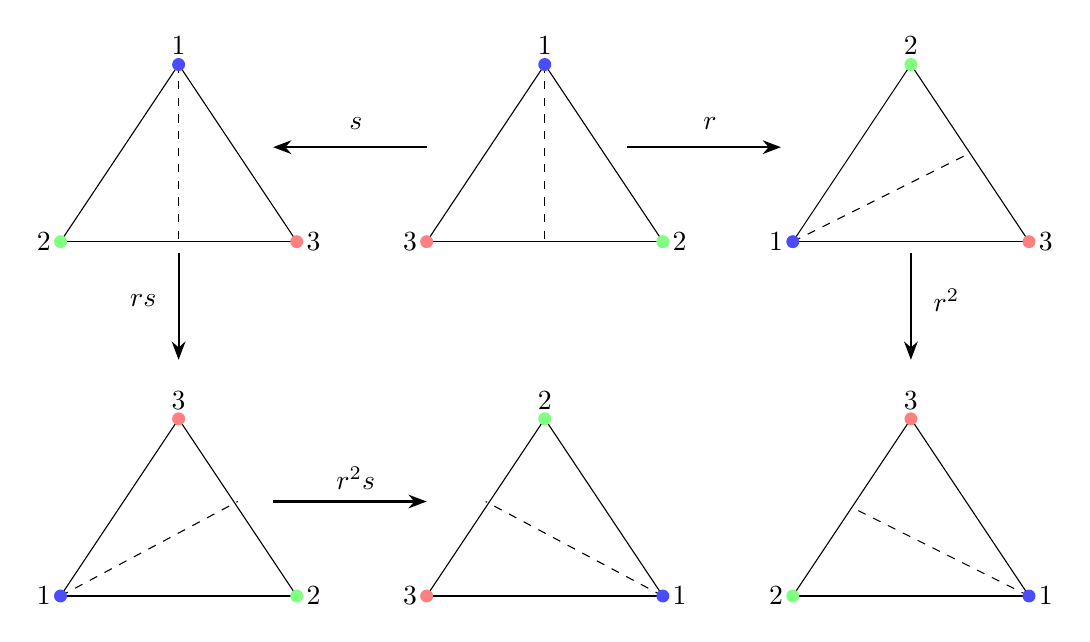
\begin{tikzpicture}[black, scale = 1.5]
            %left triangle
            \draw (-4.1,0) -- (-3.1,1.5) node[above] {$1$};
            \draw (-3.1,1.5) -- (-2.1,0) node[right] {$3$};
            \draw (-2.1, 0) -- (-4.1, 0) node[left] {$2$};
            \draw[dashed] (-3.1, 1.5) -- (-3.1,0);
    
            \filldraw[green!50] (-4.1, 0) circle(0.5mm);
            \filldraw[blue!70] (-3.1, 1.5) circle (0.5mm);
            \filldraw[red!50] (-2.1, 0) circle (0.5mm);
    
            %s arrow
            \draw[thick, <-] (-2.3,0.8) to (-1,0.8) node at (-1.6,
            1.0) {$s$};

            %middle left triangle
            \draw (-4.1,-3) -- (-3.1,-1.5) node[above] {$3$};
            \draw (-3.1,-1.5) -- (-2.1,-3) node[right] {$2$};
            \draw (-2.1, -3) -- (-4.1, -3) node[left] {$1$};
            \draw[dashed] (-4.1, -3) -- (-2.6,-2.2);
    
            \filldraw[blue!70] (-4.1, -3) circle(0.5mm);
            \filldraw[red!50] (-3.1, -1.5) circle (0.5mm);
            \filldraw[green!50] (-2.1, -3) circle (0.5mm);
    
            %sr arrow
            \draw[thick, ->] (-3.1, -0.1) to (-3.1, -1) node at (-3.4,
            -0.5) {$rs$};

                    %middle center triangle.
                    \draw (-1,-3) -- (0,-1.5) node[above] {$2$};
                    \draw (0,-1.5) -- (1,-3) node[right] {$1$};
                    \draw (1, -3) -- (-1, -3) node[left] {$3$};
                    \draw[dashed] (1, -3) -- (-0.5,-2.2);
            
                    \filldraw[red!50] (-1, -3) circle(0.5mm);
                    \filldraw[green!50] (0, -1.5) circle (0.5mm);
                    \filldraw[blue!70] (1, -3) circle (0.5mm);
                    
                    %r arrow
                    \draw[thick, ->] (-2.3,-2.2) to (-1,-2.2) node at (-1.6,
                    -2) {$r^2s$};
    
            %center triangle
            \draw (-1,0) -- (0,1.5) node[above] {$1$};
            \draw (0,1.5) -- (1,0) node[right] {$2$};
            \draw (1, 0) -- (-1, 0) node[left] {$3$};
            \draw[dashed] (0, 1.5) -- (0,0);
    
            \filldraw[red!50] (-1, 0) circle(0.5mm);
            \filldraw[blue!70] (0, 1.5) circle (0.5mm);
            \filldraw[green!50] (1, 0) circle (0.5mm);
            
            %r arrow
            \draw[thick, ->] (0.7,0.8) to (2,0.8) node at (1.4,
            1.0) {$r$};
            
            %right triangle
            \draw (2.1,0) -- (3.1,1.5) node[above] {$2$};
            \draw (3.1,1.5) -- (4.1,0) node[right] {$3$};
            \draw (4.1, 0) -- (2.1, 0) node[left] {$1$};
            \draw[dashed] (2.1,0) -- (3.6, 0.75);
    
            \filldraw[blue!70] (2.1, 0) circle(0.5mm);
            \filldraw[green!50] (3.1, 1.5) circle (0.5mm);
            \filldraw[red!50] (4.1, 0) circle (0.5mm);

            %r^2 arrow
            \draw[thick, ->] (3.1,-0.1) to (3.1,-1) node at (3.4,
            -0.5) {$r^2$};

            %middle right triangle
            \draw (2.1,-3) -- (3.1,-1.5) node[above] {$3$};
            \draw (3.1,-1.5) -- (4.1,-3) node[right] {$1$};
            \draw (4.1, -3) -- (2.1, -3) node[left] {$2$};
            \draw[dashed] (4.1,-3) -- (2.6, -2.25);
    
            \filldraw[green!50] (2.1, -3) circle(0.5mm);
            \filldraw[red!50] (3.1, -1.5) circle (0.5mm);
            \filldraw[blue!70] (4.1, -3) circle (0.5mm);


        \end{tikzpicture}
    \end{figure}
\begin{thm}
    Let $(G, \cdot)$ be a group. Then the following hold:
    \begin{itemize}
        \item[1.] The identity $e \in G$ is unique
        \item[2.] The inverse $g^{-1} \in G$ is unique for every $g
        \in G$.
        \item[3.] For any $g \in G$, $(g^{-1})^{-1} = g$. 
        \item[4.] Let $g, h \in G$. Then $(g \cdot h)^{-1} = h^{-1} \cdot g^{-1}$.   
        \item[5.] Let $g_1, g_2, \dots, g_n \in G$. The product $g_1
        \cdot g_2 \cdot \vspace{0.01mm} \dots \vspace{0.01mm} \cdot
        g_n$ is independent of its bracketing. 
        \item[6.] Let $g, h \in G$. There always exist $x, y$ such
        that $g \cdot x = h$ and $h \cdot y = g$.
    \end{itemize}
\end{thm}

\begin{prf}
    \begin{description}
        \item[1.] Suppose there exists another identity 
        element $f$, different from $e$, such that
        $g \cdot f = f \cdot g = g$ for all $g \in G$. Then 
        \[
            e = e \cdot f = f
        \]
        so that $e = f$. Therefore, the identity element is unique.

        \item[2.] Suppose $h_1$ and $h_2$ are both inverses of $g \in
        G$. Then by definition, $h_2 \cdot g = e = g \cdot h_2$ and $h_1 \cdot g = e
        = g \cdot h_1$. Therefore, 
        \[
            h_1 = (h_2 \cdot g) \cdot h_1 = \underbrace{h_2 \cdot (g \cdot h_2)}_{\text{by associativity of G}}
            = h_2 \cdot e = h_2.
        \]
        Thus $h_1 = h_2$, so that the inverse of $g$ os unique. 

        \item[3.] Observe that for any $g \in G$,
        \[
            g^{-1}\cdot (g^{-1})^{-1} = e
        \]
        by defintion. Multiplying on the left by $g$ on both sides of
        the equation, we get 
        \begin{align*}
            g \cdot (g^{-1} \cdot (g^{-1})^{-1}) = g \cdot e
            \implies (g \cdot g^{-1}) \cdot (g^{-1})^{-1} = g 
        \end{align*}
        by associativity. Since $g \cdot g^{-1} = e$, this then leads to 
        \begin{align*}
            e \cdot (g^{-1})^{-1} = g \implies (g^{-1})^{-1} = g
        \end{align*}
        as desired.

        \item[4.] Note that $(g \cdot h)^{-1} \cdot (g \cdot h) = e.$
        Therefore,
        \[
            (g \cdot h)^{-1} \cdot (g \cdot h) = e \implies (g \cdot h)^{-1} \cdot g = h^{-1}
            \implies (g \cdot h)^{-1} = h^{-1} \cdot g^{-1}
        \] 
        by first multiplying on the right by $g^{-1}$ and then by
        $h^{-1}$, which proves the formula.

        \item[5.] We can demonstrate this by induction. First write
        our proposition as
        \[
            P(n)
            =
            \begin{cases}
            \text{For any } g_1, g_2, \dots, g_n \in G\text{ we have that }\\
             g_1\cdot g_2 \cdots g_n \text{ is independent of its bracketing. }
            \end{cases}
        \] 
        \begin{description}
            \item[Base Case.]
            For the base case $n = 1$, there is nothing to check.
            \item[Inductive Step.]
            Now suppose that $P(n)$ is true for all positive integers
            $n \le n_0$. Then let $g_1, g_2, \dots g_{n+1}
            \in G$ and consider 
            \[
                g_1\cdot g_2 \cdots \cdot g_{n+1}.
            \]
            Observe that we clearly have that 
            \[
                g_1\cdot g_2 \cdots \cdot g_{n+1}. = (g_1\cdot g_2 \cdots \cdot g_{i})\cdot(g_{i+1} \cdots \cdot g_{n+1}).
            \]
            for all $1 \le i le n + 1$. Hence we can apply the
            inductive hyptohesis to each of the subproducts $(g_1\cdot
            g_2 \cdots \cdot g_{i})$ and $(g_{i+1} \cdots \cdot
            g_{n+1})$ generated
            in each case. Since this exhausts all possible
            subproducts, and the values do not change by our inductive
            hypothesis, we see that $P(n + 1)$ is true. Hence $P(n)$
            holds for all $n \in \mathbb{N}$. 
        \end{description}

        \item[6.] Observe that if we have the equation $g \cdot x =
        h$, then we can multiply both sides on the right by $g^{-1}$
        to observe that 
        \[
            (g^{-1} \cdot g) \cdot x = g^{-1} \cdot h \implies x = g^{-1} \cdot h.
        \]
        Since $x$ is the product of elements of $G$ (namely, $g^{-1}
        \cdot h$) and because $G$ is closed under $\cdot$, we have
        that $x \in G$. Thus a solution exists in $G$. The proof for
        the existence of $y \in G$ such that $h \cdot y = g$ is
        exactly the same.
    \end{description}
\end{prf}

In our study of group theory, many of the groups we'll deal with will
actually turn out to be finite. We'll also be interested in breaking
down the structures of finite groups (a lot of things can happen). 
A couple things should be noted about finite groups.

{\color{MidnightBlue}
Consider $g \in G$, where $G$ is a \textbf{finite group}. Since $G$ must be
closed under its product, we note that $g^2 \in G$, $g^3 \in G$, and so
on. That is, all powers of $g$ must be in $G$. But since $G$ is
\textit{finite}, there must exist some $m \in
\mathbb{N}$ such that $g^m = e$. If not, you could keep raising the
power of $g$, and keep getting new elements. Since you'd never come
back to $e$, you could then generate an infinite set
$\{g, g^2, g^3, g^4, \dots\}$ entirely contained in $G$. But this
would imply $G$ is infinite, which it isn't.}

\noindent
\begin{definition}
    Let $G$ be a group. The \textbf{order of an element} $g \in G$ is
    the smallest integer $n$ such that $g^n = e$. 

    In addition, if $G$ is a finite group, then we can also talk about
    the \textbf{order of a group} $|G|$, which we define as the number of
    elements within the group.
    
    The order is denoted
    as $|g|$; thus we'd say that $|g| = n$ if $g$ has order $n$. If
    $G$ is infinite, it may be possible that $|g| = \infty$. On the
    topic of order, we define that $g^0 = e$.
\end{definition}
\subsection*{Subgroups.}
    \begin{definition}
        Let $G$ be a group, and consider a subset $H$ of $G$. We define
    $H$ to be \textbf{subgroup} of $G$ if $H$ is also a group.
    \end{definition}
    
    {\color{blue}The definition is exactly what it sounds like: $H$ is a subgroup
    if $H \subset G$ and $H$ is a group. You might note that the
    definition is clear, but determining if a set is a subgroup of $G$
    sounds like a lot of work. Fortunately there's the subgroup test.
    }

    \begin{thm}\label{subgroup_test}
        Let $H$ be nonempty and suppose $H \subset G$. Then $H$ is a
        subgroup if and only if for all $x, y \in H$, $xy^{-1} \in H$.
    \end{thm}

    
    

    \noindent \textbf{If $\mathbf{H}$ is a subgroup, we usually write $\mathbf{H \le G}$ if we
    are trying to be concise.}

    \begin{prf}

        ($\implies$) Suppose $H \le G$. Then since $H$ is a group,
        for any $x, y \in H$, $xy^{-1} \in H$ since it is closed under
        multiplication of its elements. This proves the forward
        direction.
        \\
        
        ($\impliedby$) Suppose $H$ is nonempty and $H \subset G$ such
        that for all $x, y \in H$, $xy^{-1} \in H$. We just need to
        prove $H$ is a group. We already know group multiplication is
        an associative, binary operation on $G$, so it is still
        associative on elements of $H$. Thus we only need to prove
        closedness, existence of identity and inverses.
        
        By the definition of $H$, for all $x, y \in H$, $xy^{-1} \in
        H$. 
        \begin{description}
            \item[Identity.] Let $x \in H$. Then clearly $xx^{-1} = e \in H$. Thus $H$
            has the identity.
            \item[Inverses.] Since $x, e \in H$, we see that $ex^{-1} =
            x^{-1} \in H$. Thus for all $x \in H$, $x^{-1} \in H$.
            \item[Closedness.] Now let $y \in H$; hence, $y^{-1} \in H$, as just proven. Then
            $x(y^{-1})^{-1} = xy\in H$, so that $H$ is closed under
            multiplication of its elements.
        \end{description} 
        Therefore $H$ is (1) a group
        and (2) a subset of $G$ so that $H \le G$, as desired.
    \end{prf}

    It turns out the intersection of two subgroups is still a
    subgroup. In fact, the arbitrary intersection of subgroups always
    produces a subgroup. 
    \begin{thm}
        Let $G$ be a group and $\{H_\alpha\}_{\alpha \in \lambda}$ be
        a family of subgroups of $G$. Then the set $H =
        \bigcap_{\alpha \in \lambda} H_\alpha$ is a subgroup of $G$.
    \end{thm}

    \begin{prf}
        First, observe that 
        \[
            H = \bigcap_{\alpha \in \lambda} H_\alpha
        \]
        is nonempty. This is because each $H_\alpha \le G$ and thus
       the identity of $G$ is contained in each $H_\alpha$ for all
       $\alpha \in \lambda$. So the identity is in $H$ as well.

       Thus let $x, y \in H$. Then $x, y \in H_\alpha$ for all $\alpha
       \in \lambda$. Since each $H_\alpha$ is a group, $y^{-1}$ exists
       and is contained in each $H_\alpha$. Hence, $xy^{-1} \in
       H_\alpha$ for all $\alpha \in \lambda$, so we have that
       $xy^{-1} \in H$. Therefore, we see by the subgroup text that $H
       \le G$. 
    \end{prf}
    With the basic properties of a group introduced, we now introduce
    two more group definitions. 

    \begin{definition}
        Let $G$ be a group and $S \subset G$. The \textbf{centralizer}
        of $S$ in $G$ is defined to be the set $C_G(S)$
        \[
            \textcolor{NavyBlue}{C_G(S)} = \{g \in G \mid gs = sg \text{ for all } s \in S\}.
        \]
    \end{definition}
    In the case where $G$ is abelian, we $C_G(S) = G$ for any nonempty
    subset $S$ of $G$. This definition is close to the \textbf{center
    of a group}, which is as follows.

    \begin{definition}
        Let $G$ be a group. Then the \textbf{center of a group} $G$ is
        defined as 
        \[
            Z(G) = \{z \in G \mid zg = gz \text{ for all } g \in G\}.
        \]
    \end{definition}

    In this case, we note that $C_G(G) = Z(G)$ and if $G$ is abelian
    $Z(G) = G$. Finally, we introduce the definition of the
    normalizer.
    
    \begin{definition}
        Let $G$ be a group and $S \subset G$. The \textbf{normalizer}
        of $S$ in $G$ is defined as 
        \[
            \textcolor{purple}{N_G(S)} = \{g \in G \mid gS = Sg\}
        \]
    \end{definition}
    
    The centralizer and the normalizer are closely related
    definitions. However, these two concepts highlight the important
    distinction one must understand between term-by-term equality and
    set equality. \textcolor{NavyBlue}{Firstly, we can think of $C_G(S)$ as all $g \in G$
    which commutes with each and every single element of $S$.} 
    \textcolor{purple}{On the
    other hand, if $g \in N_G(S)$, it is not necessarily true that $gs
    = sg$ for all $s \in S$. The only requirement is that $gS$
    creates the same set as $Sg$. Of course, one way to do this is
    if $gs = sg$ for all $s \in G$. In that case, $gS = Sg$. But there
    are other ways to do this, so this definition is more versatile
    than $C_G(S)$.}

    One interesting fact is that $C_G(S)$ and $N_G(S)$ are subgroups
    of $G$ for any $S \subset G$. 

    \begin{thm}
        Let $G$ be a group and $S \subset G$. Then $C_G(S)$ and
        $N_G(S)$ are both subgroups of $G$.
    \end{thm}
    \textcolor{blue}{Note: if we let $S = G$, we see that $C_G(S) =
    Z(G)$. 
    Therefore, an immediate corollay of this theorem is that $Z(G)$ is
    also a subgroup of $G$!}

    \begin{prf}
        Let $G$ be a group and $S \subset G$. To show that $C_G(S) \le
        G$, we can use the subgroup test. 
        \begin{description}
            \item[Nonempty.] First we have to show the set is
            nonempty. But note that for any $S$, $e \in C_G(S)$ 
            since $gs = sg$ for any $s \in S$.

            \item[Inverses.] We now show that if $x, y \in C_G(S)$
            then so is $xy^{-1}$. We know that for all $s \in S$, $xs
            = sx$ and $ys = sy$. Therefore $s = y^{-1}sy$ and $s =
            ysy^{-1}$ by solving for $s$ in the last equation.
            Plugging this into the first equation with $x$, we get 
            \[
                xs = sx \implies x(y^{-1}sy) = (ysy^{-1})x 
                \implies xy^{-1}sy = ysy^{-1}x.
            \]
            Multiplying both sides on the right by $y^{-1}$ leads to 
            \[
                xy^{-1}s = ysy^{-1}xy^{-1} 
                \implies xy^{-1}s = syy^{-1}xy^{-1}
                \implies xy^{-1}s = sxy^{-1}
            \]
            where in the second step we used the fact that $ys = sy$.
            Thus $xy^{-1} \in C_G(S)$, so by subgroup test we have
            that $C_G(S) \le G$. 
        \end{description}

        The proof for $N_G(S)$ is the exact same; simply replace $s$
        with $S$.
    \end{prf}

    \newpage
    \section{Permutation Groups.}
    One of the most important and well-known types of groups are the
    permutation groups, which we introduce formally as follows. 

    Consider a finite set of elements $X = \{1, 2, \dots, n\}$. We
    define a 
    \textbf{permutation} to be a reordering of the elements of $X$.
    More formally, a \textbf{permutation} is a bijective mapping
    $\sigma: X \to X$, similar to one that follows. 

    How can we represent this information? We generally don't use sets
    to represent permutations, since sets 
    don't care about order. That is, $\{1, 2, 3\} = \{3,2,1\}$, etc.  

    Thus for a set $\{1, 2, \dots, n\}$, we can represent a
    permutation $\sigma$ of the set of elements as follows:
    \[
       \sigma =  
       \begin{pmatrix}
            1 & 2 & \cdots & n\\
            \sigma(1) & \sigma(2) & \cdots & \sigma(n)
         \end{pmatrix}
    \]
    where we read this as $1$ is assigned to $\sigma(1)$, 2 is
    assigned to $\sigma(2)$. For example, a permutation that just
    shifts the elements down the line is 
    \[
        \sigma = 
        \begin{pmatrix}
            1 & 2 & \cdots & n\\
            2 & 3 & \cdots & 1
         \end{pmatrix}.
    \]
    That is, $\sigma$ sends 1 to 2, 2 to 3 and eventually $n$ to 1. 
    Here we'll denote the set of all permutations of the set $\{1, 2,
    \dots, n\}$, or more generally a set of $n$ objects (since we can
    always enumerate objects with natural numbers) as $S_n$.
    
    \textcolor{NavyBlue}{What is interesting about this is that if we define
    "multiplication" of elements of $S_n$ to be function composition,
    then the 
     \textbf{set of permutations
    of $X$ form a group} which we show as follows.}
    
    Let $X = \{1, 2, \dots, n\}$. 
    \begin{description}
        \item[Closed.]
        For any $\sigma_1, \sigma_2 \in S_n$, we see that $\sigma_2
        \circ \sigma_1$ is (1) a composition of bijective functions
        and therefore is bijective and (2) a permutation of $X$. One
        way to think about the composition is that $\sigma_1$
        rearranges $X$, and
        $\sigma_2$ rearranges $X$ again. Thus $\sigma_2 \circ \sigma_1
        \in S_n$. 

        \item[Associativity.]
        Associativity is obvious since function composition is
        associative. 

        \item[Identity.]
        Observe that the permutation $\sigma_e: X \to X$ for which 
        $\sigma_e(i) = i$ is technically a permutation of $X$.
        Therefore $\sigma_e$ acts as the identity element in $S_n$. 

        \item[Inverse.]
        Consider a permutation $\sigma \in S_n$. Define $\sigma^{-1}$
        to be the function where if $\sigma(i) = j$, then
        $\sigma^{-1}(j) = i$. Then by construction, (1) $\sigma^{-1}$ is a permutation
        of $X$ and (2) $\sigma \circ \sigma^{-1} = \sigma^{-1} \circ
        \sigma = \sigma_e$. Thus $S_n$ contains inverses and
        composition of the inverses returns $\sigma_e$, the identity.
    \end{description}

    \begin{proposition}
        For all $n \ge 1$, $|S_n| = n!$ 
    \end{proposition}

    \begin{prf}
        This is counting the number of ways to rearrange a set of size
        $n$, which we know from combinatorics to simply be $n!$
    \end{prf}

    Now that we know that $S_n$ is a group, we'll study the properties
    of this group. 

    Recall earlier our notation for representing a permutation $\sigma
    \in S_n$:
    \[
       \sigma =  
       \begin{pmatrix}
            1 & 2 & \cdots & n\\
            \sigma(1) & \sigma(2) & \cdots & \sigma(n)
         \end{pmatrix}
    \]
    This notation sucks, since it includes more information than we
    actually need to. For instance, the top row is always going to be
    the same. 
    
    A better way to write this is through
    \textit{cycle decomposition}, which we will soon define.

    \begin{definition}
        Let $\sigma \in S_n$ and suppose $X = \{1, 2, \dots, n\}.$ 
        Suppose that there exists a subset $\{n_1, n_2, \dots, n_k\}$
        of $X$
        such that 
        \begin{align*}
            \sigma(n_1) = n_2, \sigma(n_2) = n_3, \dots, \sigma(n_k) = n_1.
        \end{align*}
        Then $\{n_1, n_2, \dots, n_k\}$ is called a 
        \textbf{cycle},
        and we denote this cycle as 
        \[
            \sigma = \begin{pmatrix}
                n_1 & n_2 & \cdots & n_k
            \end{pmatrix}.
        \]
        We then read this as "$n_1 \to n_2$, $n_2 \to n_3, \dots, n_k
        \to n_1$". 

        \textcolor{Blue}{\textbf{Why do we care about cycles?}} 
        \\
        Well,
        consider an arbitrary cycle $            \sigma = \begin{pmatrix}
            n_1 & n_2 & \cdots & n_k
        \end{pmatrix}.$ Then again, $\sigma(n_1) = n_2, \sigma(n_2) =
        n_3, \dots, \sigma(n_k) = n_1.$ However, what this is really
        saying is that 
        \[
            \sigma(n_1) = n_2, \sigma^2(n_1) = n_3, \dots, \sigma^{{k-1}}(n_1) = n_k, \sigma^k(n_1) = n_1.
        \]
        However, also take a note to observe that 
        \[
            \sigma(n_2) = n_3, \sigma^2(n_2) = n_4, \dots, \sigma^{{k-1}}(n_2) = n_1, \sigma^k(n_2) = n_2.
        \]
        More generally, we see that \textcolor{blue}{the element $\sigma \in S_n$ has
        order $n_k$}, which is why the cycle length is $k$. 

        \textcolor{Blue}{\textbf{We care about cycles}} since, given the fact that $S_n$
        is always a finite group, each of its elements will have
        finite order. Thus, in some way, we can always represent the
        elements of $S_n$ in this form.
        \\
        \\
        \textbf{More definitions.}
        \\
        If $            \begin{pmatrix}
            n_1 & n_2 & \cdots & n_k
        \end{pmatrix}$ and $            \begin{pmatrix}
            n'_1 & n'_2 & \cdots & n'_k
        \end{pmatrix}$ 
        share no elements in common, i.e., 
        \[
            \{n_1, n_2, \dots, n_k\} \cap \{n_1', n_2', 
            \dots, n_k'\} = \varnothing
        \]

        then the cycles are defined as
        \textbf{disjoint cycles}.
        \\

        Note that if $\sigma(i) = i$ for some $i \in X$, then this is
        technically a cycle and we represent the cycle as $            \begin{pmatrix}
            i
        \end{pmatrix}.$ In this case, we say that $\sigma$ \textbf{fixes} $i$.
        \\

        For example, suppose we have a permutation $\sigma \in S_5$
        where $\sigma(1) = 2, \sigma(2) = 4, \sigma(4) = 2$. Then we
        have a cycle of length 4 and we denote this as 
        \[
            \begin{pmatrix}
                1 & 2 & 4
            \end{pmatrix}.
        \]
        Since $\sigma \in S_5$, suppose further
        that $\sigma(3) = 5$ and $\sigma(5) = 3$. Then we see that we
        have another cycle, disjoint with the previous cycle, and we write this one as
        \[
            \begin{pmatrix}
                3 & 5
            \end{pmatrix}.
        \]
        To write the entire permutation, we then can then express
        $\sigma$ as 
        \[
            \sigma =  \begin{pmatrix}
                1 & 2 & 4
            \end{pmatrix}
            \begin{pmatrix}
                3 & 5
            \end{pmatrix}
        \]
        which gives us all the information we need to know on how
        $\sigma$ rearranges the elements of $X$. Such a representation
        of a permutation is called a \textbf{disjoint cycle decomposition}. 
        It will turn out that
        we can actually express \textit{every} permutation $\sigma \in
        S_n$ in a product of disjoint cycles.
    \end{definition}
    \textbf{Remark.}
    In general, 1-cycles are omitted in the representation of a
    disjoint cycle decomposition. Thus if we have a permutation
    $\sigma \in S_3$ such that $\sigma(1) = 2$, $\sigma(2) = 1$ and
    $\sigma(3) = 3$, then we would write this as 
    \[
        \sigma = \begin{pmatrix}
            1 & 2
        \end{pmatrix}.
    \]
    Such a statement leads us to conclude that $\sigma(3) = 3$. And if
    $\sigma \in S_5$, we would furthermore conclude that not only $\sigma(3) =
    3$, but also $\sigma(4) = 4$ and $\sigma(5) = 5$.
    \\
    \\
    \textbf{Nonuniqueness.}
    One thing to note is that cycles are not unique. For example, we
    could have written the cycle $\textcolor{ForestGreen}{\begin{pmatrix}
        1 & 2 & 4
    \end{pmatrix}} $ as $\textcolor{OrangeRed}{\begin{pmatrix}
        2 & 4 & 1
    \end{pmatrix}}$ or $\textcolor{Cyan}{\begin{pmatrix}
        4 & 1 & 2
    \end{pmatrix}}$, since the other expressions still capture the fact
    that 1 is sent to 2, 2 is sent to 4, and 4 is sent to 1. 
    \begin{center}
        \begin{tikzcd}
            & 4 \arrow[dr, color = Cyan] & \\
            2 \arrow[ur, color = OrangeRed] & & 1\arrow[ll, color = ForestGreen]
            \end{tikzcd}.
    \end{center}
    Note that the colors correspond to where the cycle starts. Clearly
    in the diagram, there are three ways to start the cycle, and hence
    why there are three nonunique representations for the cycle. 
    \\
    More
    generally, for any cycle $            \begin{pmatrix}
        i_1 & i_2 & \cdots & i_n
    \end{pmatrix}$ we have that 
    \[
        \begin{pmatrix}
            i_1 & i_2 & \cdots & i_n
        \end{pmatrix}
        = \begin{pmatrix}
            i_2 & i_3 & \cdots & i_n & i_1
        \end{pmatrix}
        = 
        \cdots 
        = 
        \begin{pmatrix}
            i_n & i_1 & \cdots & i_{n-1}
        \end{pmatrix}.
    \]





    \newpage
    \section{Homomorphism and Isomorphisms.} 
    {\color{BlueViolet}As with all mathematical objects, now that we have a well defined
    abstract concept (i.e., a group) we'll now be interested
    attempting to understand \textit{mappings} between different
    groups. Mappings of abstract concepts simply helps mathematicians
    get a better sense of what they're dealing with, and most often
    provides new insight into understand their objects. 
    
    The most important utility of the following definition is that it
    not only leads one to have a better understanding of groups, but it
    also helps us understand when two groups are equivalent. For
    example, $D_3$ and $S_3$ equivalent, since one could view $D_3$
    as simply all the permutations of 1, 2, and 3, if we assigned these
    numbers to the vertices of a triangle.
    }

    \begin{definition}
        Let $(G, \cdot)$ and $(G', *)$ be groups. A
        \textbf{homomorphism} is a mapping $\phi: G \to G'$ such that,
       for all $a, b \in G$, 
        \[
            \phi(a \cdot b) = \phi(a) * \phi(b).
        \]
        {\color{red}Again, here $*$ is the group operation of $G'$.}

    \end{definition}

    \textbf{Example.} Consider the two groups $GL_n(\mathbb{R})$ and
    $\mathbb{R}\setminus\{0\}$. If we define $\phi$ such that, for $A \in
    GL_n(\mathbb{R})$ 
    \[
        \phi(A) = \det(A)
    \]
    then $\phi$ defines a homomorphism. 
    
    Recall that for for any $n
    \times n$ matrices $A, B$ that $\det(AB) = \det(A)\det(B)$.
    Therefore 
    \[
        \phi(AB) = \det(AB) = \det(A)\det(B) = \phi(A)\phi(B).
    \]
    Since $\phi(AB) = \phi(A)\phi(B)$, we see that $\phi$ satisfies
    the condition to be a homomorphism.

    \begin{proposition}
        Let $\phi: G \to G'$ be a homomorphism. Then all of the
        following hold.
        \begin{itemize}
            \item[1.] If $e_G$ is the identity of $G$ and $e_{G'}$ is
            the identity of $G'$, then $\phi(e_G) = e_{G'}$.

            \item[2.] For all $g \in G$, $\phi(g^{-1}) =
            \phi(g)^{-1}$. 

            \item[3.] For $g_1, g_2, \dots, g_n \in G$, then $\phi(g_1
            \cdot g_2 \cdot \dots \cdot g_n) =
            \phi(g_1)\phi(g_2)\cdots\phi(g_n)$. Consequently, if $g = g_1 =
            g_2 = \cdots = g_n$, then $\phi(g^n) = \phi(g)^{n}$.
        \end{itemize}
    \end{proposition}

    \begin{prf}
        Let $g \in G$, and suppose $\phi: G \to G'$ is a
        homomorphism. 
        
        \begin{itemize}
            \item[1.] Since $e_G = e_G \cdot e_G$, we have that 
            \[
                \phi(e_G) = \phi(e_G \cdot e_G) = \phi(e_G)\phi(e_G).
            \] 
            We also know that $\phi(e_G) \in G'$, and becuase $G'$ is a group,
            there exists an inverse $\phi(e_G)^{-1} \in G$ of
            $\phi(e_G)$. Multiplying this on the left (or right)
            yields
            \[
                e_{G'} = \phi(e_G)  
            \]
            as desired.
            \item[2.] Since $gg^{-1} = e_G$, and by (1.) we know that
            $\phi(e_G) = e_{G'}$. Hence 
            \[
                \phi(e_G) = e_{G'} \implies \phi(gg^{-1}) = e_{G'} 
                \implies \phi(g)\phi(g^{-1}) = e_{G'}.
            \]
            Again, $\phi(g) \in G'$, and since $G'$ is a group there
            exist an inverse $\phi(g)^{-1} \in G$ of $\phi(g)$.
            Multiplying on the left by this inverse, we get 
            \[
                \phi(g)\phi(g^{-1}) = e_{G'} \implies \phi(g^{-1}) = \phi(g)^{-1}
            \]
            as desired.

            \item[3.] This is just repeated application of the
            homomorphism property. 
            For $g_1, g_2, \dots g_n \in G$, $g_1 \cdot
            g_2 \cdot \hspace{0.01mm} \dots \hspace{0.01mm} \cdot g_n = g_1 \cdot (g')$ 
            where $g' = g_2
            \cdot g_3 \cdot \hspace{0.01mm} \dots \hspace{0.01mm} \cdot g_n$. Applying the
            homomorphism property, 
            \[
                \phi(g_1 \cdot g_2 \cdot \hspace{0.01mm} \dots \hspace{0.01mm} \cdot g_n) = \phi(g_1 \cdot g') = \phi(g_1) \phi(g').
            \]
            Repeatedly applying the same idea, starting again with the
            product $g_2 \cdot g_3 \cdot \hspace{0.01mm} \dots
            \hspace{0.01mm} \cdot g_n$ yields the result. The fact
            that $\phi(g^n) = \phi(g)^n$ is follows immediately.
        \end{itemize}
    \end{prf}
    {\color{Plum} 
    If $\phi$ is a bijective homomorphism (i.e., one-to-one and
    onto) then we say that $\phi$ is an \textbf{isomorphism}.
    Furthermore, if there exists an isomorphism between two spaces
    $G$ and $G'$, then we say these spaces are \textbf{isomorphic}
    and that $G \cong G'$. As we'll soon see, isomorphisms gives
    us really nice results (hence the special terminology and
    notation). In addition, it can sometimes be difficult to tell when
    two groups $G$ and $G'$ are the same or different. Isomorphisms
    can help determine when there \textit{isn't} such an equivalence.

    As we'll see, the concept of an isomorphism is very powerful.
    However, proving it may not be that simple, and in ceratin cases
    the following theorem will be very useful.
    }

    \begin{thm}
        Let $G$ and $H$ be groups. The homomorphism $\phi: G \to H$ is an
        isomorphism if and only if there exists a homomorphism $\psi:
        H \to G$ such that $\psi \circ \phi$ is the identity map on
        $G$ and $\phi \circ \psi$ is the identity map on
        $H$.
    \end{thm}

    \begin{prf}
        ($\implies$) Suppose $\phi: G \to H$ is an isomorphism. Since
        $\phi$ is bijective, define the inverse map $\phi^{-1}: H \to
        G$ such that if $\phi(g) = g'$ then $\phi^{-1}(g') = g$. 

        Note that this is a well defined map due to the surjectivity
        and injectivity of $\phi$. To show it is a homomorphism, we
        need to demonstrate that $\phi^{-1}(h_1\cdot h_2) =
        \phi^{-1}(h_1)\phi^{-1}(h_2)$. Thus 
        observe that for $h_1, h_2 \in H$ there exist $g_1, g_2 \in G$
        such that $\phi(g_1) = h_1$ and $\phi(g_2) = h_2$. Therefore
        \[
            \phi(g_1 \cdot g_2) = h_1 \cdot h_2 \implies \phi^{-1}(h_1 \cdot h_2) = g_1\cdot g_2
            = \phi^{-1}(h_1)\cdot\phi^{-1}(h_2).
        \]
        Thus $\phi^{-1}$ is a homomorphism.

        Now observe that for all $g \in G$ we have that $\phi^{-1}
        \circ \phi(g) = g$ and for all $h \in H$, $\phi \circ \phi^{-1}(h) =
        h.$ Thus $\phi^{-1} \circ \phi$ is the identity on $G$ while
        $\phi \circ \phi^{-1}$ is the identity on $H$, which proves
        this direction.

        ($\impliedby$) Now suppose $\phi: G \to H$ is a homomorphism
        and that there exists a homomorphism
        $\psi: H \to G$ such that $\psi \circ \phi$ is the identity
        map on $G$ and $\phi \circ \psi$ is the identity map in $H$.
        In other words, $\psi$ and $\phi$ are inverses of each other. 
        Thus $\phi$ is a bijection function from $G \to H$, which
        implies that $\phi$ is an isomorphism. 
    \end{prf}
    
    We also introduce the following criteria which is frequently used
    to evaluate if a homomorphism is one-to-one and/or onto. 
    
    \begin{thm}\label{theorem_isomorph}
        Let $\phi: G \to G'$ be a homomorphism.
        Then 
        \begin{itemize}
            \item[1.] $\phi$ is one-to-one if and only if
            $\mbox{ker}(\phi)$ is trivial. That is, $\mbox{ker}(\phi) = \{e_G\}$, where $e_G$ is
            the identity of $G$.

            \item[2.] $\phi$ is onto if and only if $\mbox{im}(\phi) = G'$. 
        \end{itemize}
        Therefore, $\phi$ is an \textbf{isomorphism} if and only if
        (1) and (2) hold.
    \end{thm}

    \begin{prf}
        \begin{itemize}
            \item[1.] Suppose $\phi$ is one-to-one. By proposition
            1.1.1, we know that $\phi(e_G) = e_{G'}$. But since $\phi$
            is injective we know $e_G$ is the only element in $G$
            which is mapped to $e_{G'}$. Therefore $\mbox{ker}(\phi) =
            \{e_G\}$.

            Now suppose $\mbox{ker}(\phi) = \{e_G\}$. To show $\phi$
            is one-to-one, consider
            $g, h \in G$ such that
            \[
                \phi(g) = \phi(h).
            \]
            Multiplying both sides by $\phi(h)^{-1}$ we get 
            \[
                \phi(g)\phi(h)^{-1} = e_{G'}.
            \]
            By proposition 1.1.2, we know that $\phi(h)^{-1} =
            \phi(h^{-1})$. Since $\phi$ is a homomorphism, we can then
           combine the terms to get 
           \[
                \phi(gh^{-1}) = e_{G'}.
           \] 
           Since $\mbox{ker}(\phi) = \{e_G\}$, we see that 
           \[
                gh^{-1} = e_G \implies g = h.                
           \]
           Therefore $\phi$ is one to one.
           
           \item[2.] Suppose $\phi$ is onto. Then $\mbox{im}(\phi) = G'$
           is just another way of stating this fact. 
           
           Suppose $\mbox{im}(\phi) = G'$. Then for every element $g'
           \in G'$, there exists $g \in G$ such that $\phi(g) = g'$.
           That is, $\phi$ covers every value in $G'$ so that it is
           onto.
        \end{itemize}
        Thus, we have that a function is isomorphic if and only if it
        is one to one and onto. Hence, it is isomorphic if and only if
        (1) and (2) hold.
    \end{prf}

    We also make two common definitions for special homomorphisms. 
    \begin{definition}
        Let $G$ be a group.
        \begin{itemize}
            \item[1.] If $\phi: G \to G$ is a group homomorphism, then
            we say that $\phi$ is a \textbf{endomorphism}.
            \item[2.] If $\phi$ is a bijective endomorphism (an
            isomophic endomorphism) then we say that $\phi$ is an \textbf{automorphism}.
        \end{itemize} 
    \end{definition}

    \begin{thm}
        The set of all automorphisms of a group $G$, denoted as
        $\text{Aut}(G)$, forms a group with an operation $\circ$ of
        function composition.
    \end{thm}

    \begin{prf}
        We can prove this directly. 
        \begin{description}
            \item[Closure.] Let $\phi$ and $\psi$ be automorphisms.
            Then $\phi \circ \psi$ is (1) a homomorphism from $G \to
            G$ and (2) a bijection (as the composition of bijections
            is a bijetion).

            \item[Associativity.] In general, function composition is
            associative. 

            \item[Identity.] Let $i:G \to G$ be the identity map. The
            (1) $i$ is a group homomorphism and (2) a bijection.
            Therefore $i \in \text{Aut}(G)$ and we can set $i$ as the
            identity of the group. Note that 
            \[
                i \circ \phi = \phi = \phi \circ i   
            \]
            for any $\phi \in \text{Aut}(G)$. 

            \item[Inverse.] Let $\phi \in \text{Aut}(G)$. Construct
            the function $\phi^{-1}$ as follows. If $\phi(g) = g'$ for
            some $g, g' \in G$, then write $\phi^{-1}(g') = g$. Such
            an assignment is well-defined since  $\phi$ is a
            bijection. Hence we see that 
            \[
                \phi \circ \phi^{-1} = i = \phi^{-1} \circ \phi.
            \]
            Finally, observe that $\phi^{-1}$ is (1) a homomorphism
            and (2) a bijection, so we see that $\phi^{-1} \in
            \text{Aut}(G)$. Therefore this forms a group.
        \end{description}
    \end{prf}



    \newpage
    \section{Cyclic Groups.}
    Cyclics groups are a special type of group that are easy to
    recognize as group structures. In a cyclic group, one can always
    pinpoint a single element which can "generate" every other element
    of the group. For example, the subgroup of rotations $\{e, r, r^2,
    \dots, r^{n-1}\}$ in dihedral groups
    is cyclic. In such a subgroup, every element is simply a fininte
    power of $r$. We can then think of this subgroup as
    being generated by a single element, namely $r$.

    It will turn out later that, in every group, there will always be
    a subset of its elements such that the subset generates the whole
    group. Here, we're starting small, by just considering groups
    whose elements can be generated by \textit{one} element.

    \begin{definition}
        A group $G$ is \textbf{cyclic} if there exists an element $g
        \in G$ such that 
        \[
            G = \{g^n \mid n \in \mathbb{N}\}.
        \]
    \end{definition}
    
    A very trivial example of a cyclic group is the integers under
    addition. This is because every element in $(\mathbb{Z}, +)$ can
    be generated by the number 1 (e.g., 3 = 1 + 1 + 1, -2 $= -1 -1$).
    With the definition of cyclic groups at hand, we can introduce
    theorems about cyclic groups.

    \begin{thm}
        Let $G$ be a cyclic group, and suppose $G = \{g^n 
        | n \in \mathbb{N}\}$ for some $g \in G$. Then $|G| = |g|$.
    \end{thm}

    \begin{prf}
        Suppose $|g| = k$ where $k$ is some positive integer. Then 
        since $G = \{g^n | n \in \mathbb{N}\}$, 
        \[
            G = \{e, g, g^2, \dots, g^{k-1}\}.
        \]
        Therefore $|G| = k = |g|$. Now if $|g| = \infty$, then 
        by the same exact reasoning $|G| = \infty$.
    \end{prf}
    A consequence of this theorem is that if $|g| = \infty$, then we
    know that $g^a \ne g^b$ for any $a, b \in \mathbb{N}$ such that $a
    \ne b$. This would imply that $g^{a - b} = 1$, which otherwise 
    imply the group $G$ to have finite order; a contradiction if $|g|
    = \infty$ since this implies $|G| = \infty$.

    \begin{thm}
        Any two cyclic groups of the same order are isomorphic.
    \end{thm}

    \begin{prf}
        Let $G$ and $G'$ be two cyclic groups and suppose $|G| =
        |G'|$. Furthermore suppose that $G = \left< g\right>$ and $G'
        = \left< g' \right>$. Construct the homomorphism $\phi: G \to
        G'$ where 
        \[
            \phi(g^n) = (g')^n
        \]
        for any $n \in \mathbb{N}$. Observe that this is surjective, as
        the groups are of equal order so for any $(g')^n$ there we can
        identify the preimage to be $g^n$. This is also injective,
        since if $g_1' = g_2'$ are both elements in $G'$, then $g_1' =
        g_2' = (g')^n$ for some $n$ which corresponds to one and only
        one element in $G$; namely, $g^n$.
        As the homomorphism we constructed is surjective and
        injective, we have that $\phi$ is an isomorphism so that the
        groups are isomorphic.

        Note we could have also utilized Theorem 1.3 here, by constructing
        the homomorphism $\psi: G' \to G$ where $\psi((g')^n) = g^n$.

    \end{prf}

    We'll now move onto a more useful theorem concerning cyclic groups.

    \begin{thm}
        Let $G$ be a cyclic group. Then every subgroup of $G$ is cyclic.
    \end{thm}

    \begin{prf}
        Let $H$ be a subgroup of $G$.
        Let $m$ be the smallest integer such that $g^m \in H$. Suppose
        towards a contradiction that $H$ is not cyclic. That is, there
        exists an element $h \in H$ such that $h \ne g^{mn}$ for any
        $m \in \mathbb{N}$. 
        
        Since $h \in G$, and $G$ is a cyclic group, it must be \textit{some}
        integer power of $g$. Since $h \ne g^m$ for any $m \in
        \mathbb{N}$, 
        we know that
        there must exist $q, r \in \mathbb{Z}$ such that $h
        = g^{qm + r}$ where $0 < r < m$. 

        Now since $H$ is a group, $h^{-1} = g^{-(qm + r)} \in H$.
        Furthermore, $g^{(q+1)m} \in H$ since $H$ is closed under
        products. By the same reasoning,
        \[
            g^{(q+1)m}g^{-(qm + r)} = g^{m-r}
        \]
        is in $H$. However, this contradicts our assumption that $m$
        is the smallest positive integer such that $g^m \in H$. Thus
        by contradiction $H$ must be cyclic. 
    \end{prf}
    \textbf{Remark.}
    This proof utilizes the important idea that, if you \textit{know} $G$ is
    a group, and $g_1, g_2$ are \textit{any} two elements of $G$, then
    the product $g_1g_2 \in G$. Furthermore, if $g_1, g_2, \dots, g_n
    \in G$, then $g_1^{n_1}g_2^{n_2}\cdots g_k^{n_k} \in G$ for
    literally any powers $n_1, n_2 \dots n_k \in \mathbb{Z}$. 
    
    We used this idea by (1) observing that $g^m \in H$, so that
    $g^{(q+1)m} \in H$ for any $q \in \mathbb{Z}$ and (2) reasoning
    that $g^{(q+1)m}g^{-(qm + r)} \in H$.

    In addition, we'll offer a way to think about subgroups of a
    cyclic group $G$:
    \begin{gather}
        G = \{{\color{blue}e}, g, {\color{blue}g^2}, g^3, {\color{blue}g^4}, g^5, {\color{blue}g^6}, g^7, {\color{blue}g^8}, g^9, g^10, \dots\}\\
          \hspace{0.5cm}= \{{\color{red}e}, g, g^2, {\color{red}g^3}, g^4, g^5, {\color{red}g^6}, g^7, g^8, {\color{red}g^9}, g^{10}, \dots\}\\
          \hspace{0.5cm}= \{{\color{magenta}e}, g, g^2, g^3, {\color{magenta}g^4}, g^5, g^6, g^7, {\color{magenta}g^8}, g^9, g^{10}, \dots\}
    \end{gather}
    In the above representations, the color-highlighted powers of $g$
    form subgroups of $G$. Thus $\{{\color{blue}e}, {\color{blue}g^2},
    {\color{blue}g^4}, {\color{blue}g^6}, \dots\}$, 
    $\{{\color{red}e}, {\color{red}g^3},
    {\color{red}g^6}, {\color{red}g^9}, \dots \}$ and $\{{\color{magenta}e}, {\color{magenta}g^4},
    {\color{magenta}g^8}, \dots\}$ are
    all subgroups of $G$. Of course, this process will eventually terminate if
    $G$ is finite, but we represent the most general case above with
    the $\dots$ terms. In addition, if $G$ is finite one of the
    subgroups may turn out to be just the entire group $G$. 

    To find the exact subgroups of a cyclic group we can use the
    following theorem. 

    \begin{thm}
        Let $G$ be a finite cyclic group of order $n$. For every positive
        integer $d$ such that $d|n$, there is exactly one subgroup of
        order $d$ of $G$. These are all the subgroups of $G$. 
    \end{thm} 

    \begin{prf}
        Let $H$ be a subgroup of $G$ and suppose
        $|H| = m \le n$. We'll first show that $n \mid m$ and then
        show that for every $d \mid n$, there exists a subgroup of
        order $d$.

        By the previous theorem, we
        know that $H$ must be cyclic. Therefore $H = \{h^n \mid n \in
        \mathbb{N}\}$ for some $h \in G$. However, by Theorem 1.4, we
        also know that $|H| = |h|$, so that $h^m = e$. Therefore, 
        \[
            H = \{e, h, h^2, \dots, h^{m-1}\}.
        \] 
        However, if $G = \{e, g, g^2, \dots, g^{n-1}\}$ for some $g \in G$, then $h = g^k$ for some
        positive integer
        $k < n$. Therefore 
        \[
            H = \{g^{jk} \mid j \in \mathbb{N}\}.
        \]
        Since $g^k$ generates $H$, we can apply Theorem 1.4 to
        conclude that $|g^k| = m$. In order for this to be true, there must
        exist some positive integer $j$ such that $g^{jk} = e$.

        On one hand, we already know $m$ is the smallest such integer, as
        we specified $h^m = (g^k)^m = e$. On the other, we also know
        that $|g| = n$; that is, $n$ is the smallest integer such that
        $g^n = e$. Therefore, we have that 
        \[
            n = mk
        \]
        which proves that $m \mid n$. 

        To show that for each $d \mid n$ there exists a subgroup of
        order $d$, simply observe that if $G = \{e, g, g^2, \dots ,
        g^n\}$ then the set $\{e, g^{n/d}, g^{2n/d}, \dots,
        g^{(d-1)n/d}\}$ is a subgroup of order $d$. This completes the
        proof.
    \end{prf}

    \newpage
    \section{Left and Right Cosets, Lagrange's Theorem}

    The result of the previous proof is a special case of a more general
    theorem we'll come across, know as Lagrange's Theorem. The theorem
    states that if $G$ is a finite group and $H$ is a subgroup, then
    $|H| \mid |G|$. That is, the order of $H$ divides $G$. This is a
    remarkable and useful result, aiding proofs as we move on from it.
    But in order to reach Lagrange's Theorem we first discuss the
    extremely important concept of a \textbf{coset} of a group.

    Before defining a coset, we first recall the definition of an
    equivalence relation. 

    \begin{definition}
        An equivalence relation on a set $G$ is a binary relation
        $\sim$ that satisfies the following properties.
        \begin{description}
            \item[Reflexive.] For all $a \in G$, $a \sim a$.
            \item[Symmetric.] If $a \sim b$ then $b \sim a$.
            \item[Transitive.] If $a \sim b$ and $b \sim c$ then $a
            \sim c$. 
        \end{description}
    \end{definition}

    \textcolor{Plum}{Equivalence classes are a useful concept since they tend to break
    up a set of objects $G$ into distinct, disjoint sets $A_i$. More
    specifically, they partition $G$. These sets, $A_i$, are
    known as \textbf{equivalence classes} since their criteria for
    membership requires that $a \in A_i$ if and only if $a \sim a'$ for
    all $a' \in A_i$. 
    This is a general strategy in mathematics: to define equivalence
    classes from \textit{some} equivalence relation to break up a set
    into disjoint partitions. However, we use the
    concept of an equivalence class to partition a group $G$. We use
    the following relation to do this.}
    \\

    \textcolor{blue!90!black!100}{\textbf{The Relation.}}

    Let $G$ be a group and $H$ be a subgroup of $G$. If $a, b \in G$, then the
    relation $\sim$ on $G$ such that $a \sim b$ if and only if $ab^{-1} \in H$
    is an equivalence relation.
  \begin{prf}
    \begin{description}
        \item[Reflexive.] Observe that $a \sim a$, since $aa^{-1} = e
        \in H$.

        \item[Symmetric.] First, if $a \sim b$ then $ab^{-1} \in H$. Since $H$ is a
        group, we know that $(ab^{-1})^{-1} = ba^{-1} \in H$.
        Thus by our definition we see that $b \sim a$, so that our
        relation is also symmetric. 

        \item[Transitive.] Now suppose $a \sim b$ and $b \sim c$ for
        $a, b, c \in G$. Then by definition $ab^{-1} \in H$ and
        $bc^{-1} \in H$. Since $H$ is a group, and it is closed under
        products of its elements. Therefore
        \[
            (ab^{-1})(bc^{-1}) = ab^{-1}bc^{-1} = ac^{-1} \in H.
        \]
        Thus we see that $a \sim c$, which proves that our
        relation is transitive.
    \end{description}
\end{prf}
    As our relation is reflexive, symmetric and transitive, we see
    that it is an equivalence relation. Note however that we could
    have defined our relation as $a \sim b$ if and only if $a^{-1}b
    \in H$; such a relation is equivalent to what we just worked with.

    First we require a quick definition.
    \begin{definition}
        Consider a subgroup $H$ of $G$. For any $a \in G$, we define
        \begin{align*}
            Ha = \{ha \mid \text{ for all }h \in H\}
        \end{align*}
        to be the right coset of $H$. We also define
        \begin{align*} 
            aH = \{ah \mid \text{ for all }h \in H\}. 
        \end{align*}
        to be the left coset of $H$.
        Note that since $H$ is a group, it is closed under products of
        its elements. Therefore for any $h\in H$
        \[
            hH = Hh = H.
        \]
    \end{definition}

    \textcolor{red!80}{Don't confuse the above equality; take special note that 
    equality above is \textit{set equality}, not term by term
    equality. Of course we have no idea if $ha = ah$ where $h \in H$
    for $a \in G$ unless $G$ is abelian or we have other information.}
    \\

    \textcolor{blue!90!black!100}{\textbf{The Big Idea of Cosets.}}

    Now consider the relation introduced earlier, which we 
    proved is in fact an equivalence
    relation. Consider an equivalence class of an element $a \in G$,
    denoted $[a]$. Then we can describe $[a]$ as 
    \begin{gather*}
        [a] = \{g \in G \mid g \sim a \}\\
        \hspace{1.35cm} = \{g \in G \mid ga^{-1} \in H \}\\
        \hspace{4.2cm} = \{g \in G \mid ga^{-1} = h \text{ for some } h \in H \}\\
        \hspace{3.75cm} = \{g \in G \mid g = ha \text{ for some } h \in H \}\\
        \hspace{-1.7cm}= Ha.
    \end{gather*}
    Thus the equivalence classes of the elements of $G$ with respect
    to some subgroup $H$ are simply just the right cosets of $H$. (We
    could have alternatively defined our equivalence relation to be $g
    \sim a$ if and only if $a^{-1}g \in H$, in which case our above
    description of $[a]$ would have resulted in being equal to $aH$. Since both
    formulations are equivalent, we will simply work with the right
    cosets of $H$, namely the sets $Ha$.)

    \begin{figure}[h]
        \centering
        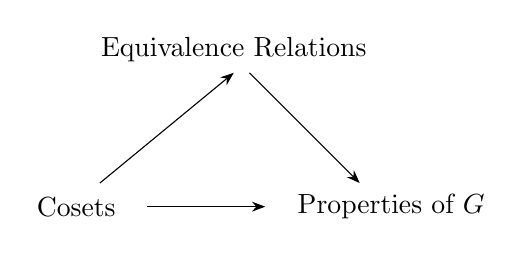
\begin{tikzpicture}
            \node at (0,0) {Cosets};
            \draw[->] (0.3, 0.3) -- (2, 1.7);
            \node at (2, 2) {Equivalence Relations};
            \draw[->] (0.9, 0) -- (2.4, 0);
            \draw[->] (2.2, 1.7) -- (3.6, 0.3);
            \node at (4,0) {Properties of $G$};
        \end{tikzpicture}
    \end{figure}
    Once we understand cosets, we can understand a lot about a group,
    because they're really 
    
    just equivalence classes!
    \vspace{0.8cm}

    \textcolor{NavyBlue!100!black!100}{Since equivalence classes are mathematical objects which partition
    a set, what we have is the following beautiful idea: We can take a
    subgroup $H$ of a set $G$ and partition our group $G$ via the
    right (or left) cosets of $H$. This is because our cosets are
    equivalence classes, and as we said before equivalence classes
    partition sets which they are defined on.}
    \\
    \\
    \textbf{Example}\\
    Consider the group $\ZZ$ and the subgroup $5\ZZ = \{5n \mid n \in \ZZ\}$. 
    We can calculate the cosets of this $\ZZ$ with respect to $5\ZZ$ as 
    \begin{align*}
        5\ZZ + 1 &= \{5n + 1 \mid n \in \ZZ\}\\
        5\ZZ + 2 &= \{5n + 2 \mid n \in \ZZ\}\\
        5\ZZ + 3 &= \{5n + 3 \mid n \in \ZZ\}\\
        5\ZZ + 4 &= \{5n + 4 \mid n \in \ZZ\}\\
        5\ZZ + 5 &= \{5n + 5 \mid n \in \ZZ \} = 5\ZZ
    \end{align*}
    Note that we didn't list any other
    cosets. Well, that's because these are all of the possible
    distinct cosets of $\ZZ$ with respect to $5\ZZ$. For example, the coset $5\ZZ + 37$ is
    equivalent to $5\ZZ + 2$, since 
    \begin{align*}
        5\ZZ + 37 = \{5n + 37 \mid n \in \ZZ\}
        &= \{5n + 5\cdot 7 + 2 \mid n \in \ZZ\}\\
        &=\{5(n+7) + 2 \mid n \in \ZZ\}\\
        &= 5\ZZ + 2.
    \end{align*}
    Thus, any other coset we propose is equivalent to one of the five
    we listed. This is demonstrated in the figure below.

    \begin{figure}[h]
        \centering
        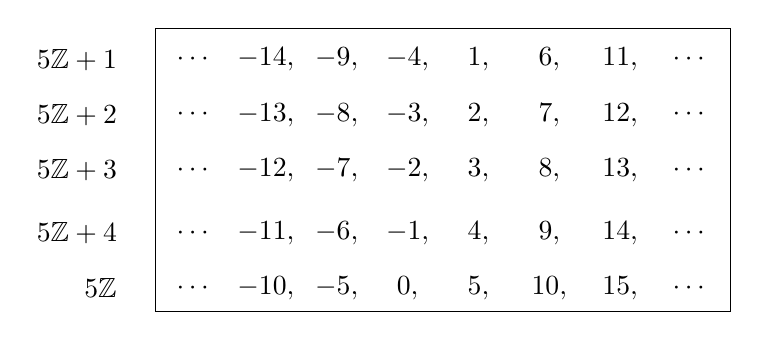
\begin{tikzpicture}
            \node at (-1,3.2) {$5\ZZ + 1$};
            \node at (-1,2.5) {$5\ZZ + 2$};
            \node at (-1,1.8) {$5\ZZ + 3$};
            \node at (-1,1) {$5\ZZ + 4$};
            \node at (-0.7,.3) {$5\ZZ$};

            \draw (0,0) rectangle (7.3,3.6);
            \node at (0.5, 3.2) {$\cdots$};
            \node at (1.4, 3.2) {$-14,$};
            \node at (2.3, 3.2) {$-9,$};
            \node at (3.2, 3.2) {$-4,$};
            \node at (4.1, 3.2) {$1,$};
            \node at (5.0, 3.2) {$6,$};
            \node at (5.9, 3.2) {$11,$};
            \node at (6.8, 3.2) {$\cdots$};

            %%%%%%%%%%
            \node at (0.5, 2.5) {$\cdots$};
            \node at (1.4, 2.5) {$-13,$};
            \node at (2.3, 2.5) {$-8,$};
            \node at (3.2, 2.5) {$-3,$};
            \node at (4.1, 2.5) {$2,$};
            \node at (5.0, 2.5) {$7,$};
            \node at (5.9, 2.5) {$12,$};
            \node at (6.8, 2.5) {$\cdots$};

            %%%%%%%%
            \node at (0.5, 1.8) {$\cdots$};
            \node at (1.4, 1.8) {$-12,$};
            \node at (2.3, 1.8) {$-7,$};
            \node at (3.2, 1.8) {$-2,$};
            \node at (4.1, 1.8) {$3,$};
            \node at (5.0, 1.8) {$8,$};
            \node at (5.9, 1.8) {$13,$};
            \node at (6.8, 1.8) {$\cdots$};

            %%%%%%%
            \node at (0.5, 1.0) {$\cdots$};
            \node at (1.4, 1.0) {$-11,$};
            \node at (2.3, 1.0) {$-6,$};
            \node at (3.2, 1.0) {$-1,$};
            \node at (4.1, 1.0) {$4,$};
            \node at (5.0, 1.0) {$9,$};
            \node at (5.9, 1.0) {$14,$};
            \node at (6.8, 1.0) {$\cdots$};

            %%%%%%%%%
            \node at (0.5, .3) {$\cdots$};
            \node at (1.4, .3) {$-10,$};
            \node at (2.3, .3) {$-5,$};
            \node at (3.2, .3) {$0,$};
            \node at (4.1, .3) {$5,$};
            \node at (5.0, .3) {$10,$};
            \node at (5.9, .3) {$15,$};
            \node at (6.8, .3) {$\cdots$};
        \end{tikzpicture}
    \end{figure}

    Note that in this figure we can identify every integer in $\ZZ$.
    This assures us that our above list of cosets is in fact complete.
    In addition, this demonstrates the fact that cosets partition a
    group. Note that each above coset is disjoint, yet the union of
    all of the cosets is the entire group $G$.
    \\
    \\
    
    As cosets can partition a group, we define $[G:H]$, called the
    \textbf{index}, to be the
    number of distinct right (or equivalently left) cosets of $G$.
    If $G$ is finite, then $[G:H]$ is of course finite. However, $G$
    can still be infinite while $[G:H]$ is finite.

    \begin{proposition}
        If $G$ is a group and $H$ is a subgroup, then for $a, b \in
        G$, $Ha \cap Hb = \emptyset$ or $Ha = Hb$.
    \end{proposition}

    This proves the observation we made beforehand in the example with
    the cosets of $\ZZ$ with respect to $5\ZZ$. We saw that the 5 cosets
    we came up with were distinct and disjoint, which is what this
    proposition proves is true in general.

    \begin{prf}
        This is simply a consequence of the connection between cosets
        and 
        equivalence relations of $G$. Equivalence classes form partitions,
        so by definition they are disjoint. However, equivalence classes
        can also be equal to one another (namely, if $a, b$ belong to the
        same equivalence class $A$, then $[a] = [b] = A$. This is why
        equivalence classes, which in our case are cosets, are
        awesome.) Therefore cosets $Ha$ and $Hb$ are either disjoint or
        equal to each other.

        This, however, can be proven directly. Consider such $Ha$ and
        $Hb$. Suppose $Ha \cap Hb \ne \emptyset$. Then by definition
        of cosets, there exists a $h_1$ and $h_2$ such that $h_1a = h_2b$.
        Therefore $a = h_1^{-1}h_2b$. Since $H$ is a group, and it is
        closed under products of its elements, there exists a
        $h'$ such that $h'= h_1^{-1}h_2$. Thus $a = h'b$.
        Consequently, we see that 
        \begin{align*}
            Ha = \{ha \mid h \in H\} = \{h(h'b) \mid h \in H\} = H(h'b).
        \end{align*}
        However, recall earlier that $Hh = H$ for any $h \in H$. Since
        $h' \in H$, we then have that 
        \[
            H(h'b) = (Hh')b = Hb
        \]
        which proves that $Ha = Hb$ as well as the proposition.
    \end{prf}

    \begin{proposition}
        Let $G$ be finite and $a, b \in G$. If $H$ is a subgroup, and 
        $Ha$ and $Hb$ are distinct cosets, then $|Ha| = |Hb|$.
    \end{proposition}
        \textcolor{red}{Hence, cosets of $G$ with respect to some
        subgroup $H$ are always of the same size.}
    \begin{prf}
        Construct a bijection $f: Ha \to Hb$ given by $f(ha) = hb$.
        Observe that this is surjective. It is also injective since
        $hb = hb'$ 
        if and only if $b = b'$, but since we assumed $Ha$ and $Hb$
        are distinct, we know by the previous proposition that
        distinctness implies disjointness. Since we can formulate a bijection
        the two sets, the sets have the same sizes.
    \end{prf}

    The next theorem, credited to Lagrange, demonstrates the
    usefulness of studying cosets to study finite groups. Our
    equivalence classes not only parition our group $G$, but they are
    also the same size. Therefore, we can always partition a finite group
    $G$ into equally sized cosets. 

    \begin{thm}
        Let $G$ be a finite group, and suppose $H$ is a subgroup of
        $G$. Then $|H|$ divides $|G|$.
    \end{thm}

    \begin{prf}
        Since $G$ is finite, there are a distinct set of cosets $Ha_1,
        Ha_2, \dots , Ha_n$ which partition $G$. By Proposition 1.3,
        each set is of equal size; call it $k$. Therefore, we see that 
        \[
            |Ha_1| + |Ha_2| + \cdots + |Ha_n| = |G|
            \implies kn = |G|.
        \]
        Therefore $|G|$ will always be a multiple of $|H|$. Or, in
        other words, $|H|$ divides $|G|$.
    \end{prf}
    
    This is the theorem we said was a more general case of Theorem
    1.6. 
    The above theorem enables us to understand all the possible
    subgroups of any finite group $G$. In fact, the theorem implies
    more useful consequences of Theorem 1.7.

    \begin{corollary}
        Let $G$ be a finite group and $H$ a subgroup of $G$. Then we
        have the following consequences: 
        \begin{enumerate}
            \item If $G$ is a finite group and $g \in G$, then $|g|$
            divides $|G|$ and $g^{|G|} = e$.

            \item Let $p$ be a prime number. 
            If $G$ is a group of order $p$, then $G$ is a cyclic
            group.
            
            \item If $ \phi :G \to G'$ is a homomorphism between finite
            groups, then $|\mbox{ker } \phi|$ divides $G$ and
            $|\mbox{im }\phi|$ divides $G'$.

            \item $|G| = |H|\cdot[G:H]$ for any subgroup $H$ of $G$.
        \end{enumerate}
    \end{corollary}

    \begin{prf}
        \begin{enumerate}
            \item Consider the cyclic subgroup $H = \left<g\right>$ of $G$. By
            Lagrange's theorem, we know that $|H|$ divides $|G|$ isnce
            $H$ is a subgroup of $G$. However $|g| = |H|$ since $H$ is
            cyclic. Therefore $|g|$ divides the order of $|G|$. This
            implies that $|G| = n|g|$ for some $n \in \mathbb{N}$.
            Therefore 
            \[
                g^{|G|} = g^{n|g|} = (g^{|g|})^n = e^n = e
            \]
            which is what we set out to show.

            \item If $|G| = p$, we know by Lagrange's Theorem we know
            that there are exactly two subgroups of $G$, namely the
            trivial group and the whole group $G$.

            Thus let $g \in G$, where $g$ is not the identity, 
            and consider the subgroup $H = \left< g
            \right>$. Since $g$ is not the identity, $H$ is not the
            trivial group. But since it is a nontrivial subgroup, and
            the only nontrivial subgroup of $G$ is itself, we see that our
            only choice is to let $H = G$. However, $H$ is cyclic,
            which proves that $G$ is cyclic as well.

            \item This result immediately follows from the fact that
            $\mbox{ker } \phi$ is a subgroup of $G$ and $\mbox{im }\phi$ is a
            subgroup of $G'$. Applying Lagrange's theorem leads to the
            result.
            
            \item For any subgroup $H$ of $G$, we know that $[G:H]$ is
            the number of left or right cosets of $G$. Since each such
            set is of size $|H|$, and because they all together
            partition $G$, we see that $|G| = |H| \cdot [G:H]$.
        \end{enumerate}
    \end{prf}
    \newpage
    \section{Normal subgroups}

    Normal subgroups are special subgroups which exhibit properties of
    interest for when we go on to later define the idea of quotient
    groups, a concept we have touched upon slightly in considering
    $\mathbb{Z}/2\mathbb{Z}$ and other modulo groups. They are a bit
    abstract at first, since they have to do with \textbf{cosets}.
    Once you work with normal subgroups for a bit, it will s
    eventually click and the reasoning behind their definitions
    becomes clear. 

    \begin{definition}
        Let $G$ be a group and suppose $H$ is a subgroup of $G$. We
        say that $H$ is \textbf{normal} if and only if \textbf{for every} $g
        \in G$, we have that $Hg = gH$. We denote such a relation as
        $H \unlhd G$.
    \end{definition}
    \noindent We make two remarks here.
    \begin{description}
        \item[Commutative Groups.] 
         
        Note that if $G$ is commutative, then $H$, a subgroup of $G$, is
        also commutative. In fact, $H$ commutes with all elements of $G$.
        That is, if $H = \{h_1, h_2, \dots \}$ then
        \[
            gH = \{gh_1, gh_2, \dots\} = \{h_1g, h_2g, \dots\} = Hg
        \]
        for all $g \in G$. Thus what we're trying to say here is if $G$ is commutative, every
        subgroup $H$ of $G$ is normal.

        \item[Set Equality.] If $H$ is normal to $G$, then $gH = Hg$
    all $g \in G$. Be careful with this equation, since what this is
    not saying is that $gh=hg$ for all $g\in G$ and $h \in H$; that
    would imply commutativity, and it may be the case that $G$ and $H$
    are not commutative groups. That is, the above equation is set
    equality, not term-by-term equality.

    What this does say, however, is if $gH = Hg$, then for each $g\in
    G$, and for every $h_1 \in H$, there exists an $h_2 \in H$ such
    that 
    \[
        gh_1 = h_2g.
    \]
    Note here that commutative groups satisfy this because in their
    case, $h_1 = h_2$ satisfies the equation. 
    \end{description}

    Since our current definition of normality would be exhausting to
    use directly if we wanted to check if a subgroup is normal, we
    have the following theorem that helps us check for normality. 

    \begin{thm}
        Let $G$ be a group and $H$ a subgroup of $G$. The following
        are equivalent:
        \begin{itemize}
            \item[1.] $H \normal G$ for all $g \in G$
            \item[2.] $gHg^{-1} = H$ for all $g \in G$
            \item[3.] $gHg^{-1} \subset H$ for all $g\in G$.
            \item[4.] $(Hg)(Hh) = H(gh)$ for all $g, h \in G$
        \end{itemize}
    \end{thm}

    \begin{prf}
        We'll prove this by producing a chain of imply statements that
        can traverse in both directions.
        Let $G$ be a group and $H$ be a subgroup. 
        
        \noindent $\mathbf{(1 \iff 2)}$ If $H \normal G$, then $gH = Hg$
        for all $g \in G$. Multiplying on the left by $g^{-1}$, we
        then see that $gHg^{-1} = H$ for all $g \in G$.

        Proving the reverse direction, if $gHg^{-1} = H$ for all $g \in G$
        then $gH = Hg$ for all $g \in G$, which means that $H$ is
        normal by defintion. 

        \noindent $\mathbf{(2 \iff 3)}$ If $gHg^{-1} = H$ for all $g \in G$
        then it is certainly true that $gHg^{-1} \subset H$ for all $g
        \in G$. 
        
        Now we prove the other direction. Suppose $gHg^{-1} \subset H$ for
        all $g \in G$. Then
        \[
            gHg^{-1} \subset H \implies gH \subset Hg 
            \implies H \subset g^{-1}Hg
        \]
        by multiplying on the right by $g$ and on the left by
        $g^{-1}$. However, since we have assumed (3) is true we know
        that 
        \[
            (g^{-1})H(g^{-1})^{-1} \subset H \implies g^{-1}Hg
            \subset H. 
        \] 
        By the above equations we then have that $H = g^{-1}Hg$, and
        multiplying by $g^{-1}$ on the right and $g$ on the left
        yields that $H = gHg^{-1}$ as desired.

        \noindent$\mathbf{(2 \iff 4)}$ Suppose (2). Then observe that $gHg^{-1} = H
        \implies gH = Hg$ for all $g \in G$.
        Therefore for $h \in G$, 
        \[
            (Hg)(Hh) = H(gH)h = H(Hg)h = H(gh).
        \]
        In the first step we used associativity and in the
        second step we used the fact that $gH = Hg$. 

        To prove the other direction, suppose $(Hg)(Hh) = H(gh)$ for
        all $g, h \in G$. Let $h = e$. Then 
    \end{prf}
    To show a subgroup $H$ of $G$ is normal, condition (3) of this
    theorem generally the fastest and easy way to take advtange of. It
    is usually the least complicated one to show. 
    \\
    \\
    \noindent
    \textbf{Example.}
    \\
    Consider the group $GL_n(\mathbb{R})$ and its subgroup
    $SL_n(\mathbb{R})$. It turns out that $SL_n(\mathbb{R}) \normal
    GL_n(\mathbb{R})$, which we will show using condition (3).

    Let $A \in GL_n(\mathbb{R})$ and suppose $T
    \in SL_n(\mathbb{R})$. We must show that $ATA^{-1} \in
    SL_n(\mathbb{R})$ for all $A \in GL_n(\mathbb{R})$ and $T \in
    SL_n(\mathbb{R})$. Observe that 
    \begin{align*}
        \det(ATA^{-1}) = \det(A)\det(T)\det(A^{-1})
        = \det(A)(1)\det(A)^{-1} = 1
    \end{align*}
    where we used the basic properties of the determinant for the
    calculation. Since $\det(ATA^{-1}) = 1$, we have that $ATA^{-1}
    \in SL_n(\mathbb{R})$ for all $A$ and $T$ in $GL_n(\mathbb{R})$
    and $SL_n(\mathbb{R})$, respectively. Therefore $SL_n(\mathbb{R})$
    is normal to $GL_n(\mathbb{R})$.   
    \\
    \\
    \textbf{Example.}
    \\
    One important example is the following: for any group homomorphism
    $\phi$ between two groups $G$ and $G'$, recall that
    $\mbox{ker}(\phi)$ is a subgroup of $G$. However, we also have
    that $\mbox{ker}(\phi) \normal G$, which we'll show as follows.

    \begin{proposition}
        Let $G, G'$ be groups and $\phi: G \to G'$ be a group
        homomorphism. Then $\ker(\phi) \normal G$.
    \end{proposition}

    \begin{prf}
        We need to show that for all $g \in G$, $h \in \mbox{ker}(\phi)$
        that $ghg^{-1} \in \mbox{ker}(\phi)$. Thus observe that 
        \[
            \phi(ghg^{-1}) = \phi(g)\phi(h)\phi(g^{-1})
            = \phi(g)\cdot 0 \cdot \phi(g^{-1}) = 0.
        \]
        Since $\phi(ghg^{-1}) = 0$, we thus see that $ghg^{-1} \in
        \mbox{ker}(\phi)$ for all $g \in G$ and $h \in \mbox{ker}(\phi)$,
        which proves $\mbox{ker}(\phi) \normal G$.    
    \end{prf}

    Another important example of normality is the fact that the
    center of a group $Z(G)$ is normal to $G$ for any group $G$.

    \begin{proposition}\label{normal_center}
        Let $G$ be a group. Then $Z(G) \normal G$.
    \end{proposition}

    \begin{prf}
        Recall that $Z(G)$ is a subgroup of $G$, consisting of all the
        elements of $G$ which commute with every element in $G$. More
        precisely, 
        \[
            Z(G) = \{z \in G \mid gz = zg \text{ for all } g \in G\}.
        \]
        Now for any $g \in G$ and $z \in Z(G)$, we have that $gzg^{-1}
        = gg^{-1}z = z$, since $z$ commutes with all elements of $G$.
        Therefore $gzg^{-1} \in Z(G) \implies gZ(G)g^{-1} \subset
        Z(G)$. By the previous theorem, we can conclude that $Z(G)
        \normal G$ as desired.
    \end{prf}

    Next, we introduce a small theorem that allows us to quickly and
    easily identify if a subgroup $H$ of $G$ is normal. 

    \begin{thm}
        If $G$ is a group and $H$ is a subgroup, and $[G:H] = 2$, then
        $H \normal G$.
    \end{thm}
    
    \begin{prf}
        Since $G$ has two right (and equivalently two left) cosets, we
        see that they must be of the form $H$ and $Hg$ where $g \in
        G\setminus H$ (that is, all of the elements of $G$ which are
        not in $H$).   

        As we said before, there are equivalently two left cosets $H$
        and $gH$ where $g \in G\setminus H$. Since the cosets partition $G$, we see that for any $g \in
        G\setminus H$ two partitions of $G$ are 
        \[
            \{H, Hg\} \hspace{0.2cm}\text{and}\hspace{0.2cm} \{H, gH\}.
        \]
        Since these partition the same set we see that $gH = Hg$ for
        all $g \in G\setminus H$. Note that we already know that for
        \    $g \in H$, $Hg = H$ and $gH = H$ so $gH = Hg$. Therefore,
        we have all together that $Hg = gH$ for all $g \in G$.
    \end{prf}

    \noindent In working with normal subgroups, one may form the following
    questions. 
    \\
    
    \textcolor{ForestGreen}{\textbf{Q:} If $K$ is a normal subgroup of $H$ and $H$ is a normal
    subgroup of $G$, is $K$ normal to $G$?}
    \\

    \textbf{A:} \textbf{Not always}. If $H \normal K$, then $khk^{-1} \in
    K$ for all $k \in K$ but there is nothing allowing for us to extend
    this further and state that $ghg^{-1} \in K$ for all $g \in G$. 
    \\
    However, a special case for when this is true involves $Z(G)$. We
    know that $Z(G) \normal G$. But if $K \normal Z(G)$ then
    it turns out $K \normal G$, 







    \newpage

    \section{Quotient Groups.}
    The work done in the previous section on Normal subgroups now
    leads to the formulation of the \textbf{Quotient Group}. Up to
    this point we've studied groups which have familiar, concerete
    objects, but now we're going to get a little bit abstract.
    We're going to look at the useful concept of the quotient group, $G/H$,
    which is a 
    \textbf{group whose elements are $H$ cosets}. That is, the elements of
    our group are going to be sets themselves. The operation on the
    elements of the quotient group can only make sense if the cosets
    are from a subgroup $H$ which is normal to $G$.

    \begin{thm}
        Let $G$ be a group and $H \normal G$. Define $G/H$ to be the
        set consisting of all the possible right (or equivalently
        left) $H$ cosets. If we
        equip this set with a product $\cdot$ such that 
        \[
            (Ha)\cdot(Hb) = H(ab)
        \]
        then $G/H$ forms a group, called the \textbf{Quotient Group}.
    \end{thm}
    Let's review what this is saying. Basically, if we have a normal
    subgroup $H$ of $G$, the set of cosets $\{Hg_1, Hg_2, \dots \}$
    with the product $Hg_1 \cdot Hg_2 = H(g_1g_2)$ \textbf{forms a group}.

    \begin{prf}
        \begin{description}
            \item[Identity.] To show that this set is a group, we first define the identity
            element to simply be $H$. This is a "trivial" coset, and for
            any $Ha$, where $a \in G$, 
            \begin{align*}
                (Ha)(H) = Ha \\
                (H)(Ha) = Ha
            \end{align*}
            so $H$ is a natural and apporopriate choice for an identity as
           it has the property of an identity element.  

           \item[Associativity.] Associativity is derived from the
           associativity of our group $G$ itself. Observe that for any
           $a, b, c \in G$ we have 
           \begin{align*}
               (Ha)[ (Hb)(Hc)] = Ha[H(bc)] = H(abc)\\
               [(Ha)(Hb)](Hc) = [H(ab)]Hc = H(abc).
           \end{align*}
           Therefore $(Ha)[ (Hb)(Hc)] = [(Ha)(Hb)](Hc)$ for all $a, b,
           c \in G$, so the product relation is associative.

           \item[Closedness.] The result of our proposed product is
           always a coset itself ($Ha \cdot Hb = H(ab)$), and since 
           $G/H$ is a set of all $H$ cosets we see that this set is
           closed under $\cdot$.

           \item[Inverses.] For any $Ha \in G/H$, where $a \in G$, we
           see that the inverse element is $Ha^{-1}$, since 
           \begin{align*}
               (Ha)(Ha^{-1}) = H(aa^{-1}) = H\\
               (Ha^{-1})(Ha) = H(a^{-1}a) = H
           \end{align*}
           and we already defined $H$ to be our identity element. So
           our proposed inverse makes sense.
           Note that
           $Ha^{-1} \in G/H$ since $a^{-1} \in G$, so an inverse
           element not only exists but it also exists in $G/H$
        \end{description}
        All together, this allows us to observe that we have a group
        structure, so long as $H \normal G$.
    \end{prf}
    {\color{purple}(Why do we need this
        the condition that $H \normal G$? Well, because the only way we can make damn sure
        that $(Ha)(Hb) = H(ab)$ is by Theorem 1.10, which requires
        that $H \normal G$.)
        }

   {\color{NavyBlue} Note that there is another way to think about $G/H$. The elements
    of the quotient group are cosets, right? However, let us not forget
   that cosets are simply \textbf{\textit{equivalence classes which
   respect the following equivalence relation}} }: {\color{Black} if $G$ is a group, $H$ is a
   subgroup, then for any $a, b \in G$ we say that $a \sim
    b$ if and only if $ab^{-1} \in H$.} {\color{NavyBlue} Thus we can
    recast our definition follows:}
    \\
    
    \begingroup
    \par
    \leftskip25pt
    \rightskip\leftskip
    \noindent Let $H \normal G$. Then the set $G/H$ is defined to consist of all
    of the
    \sout{right (or left) cosets of $H$ in $G$} equivalence classes of
    the elements of $G$ (under the equivalence relation stated in the
    previous paragraph). 
    \par
    \endgroup
    \vspace{1cm}

    {\color{Violet}We thus have two equivalent ways to interpret the meaning of a
    quotient group. One involves equivalence classes, while the other
    involves cosets. In our case it seems more complicated to think
    about equivalence classes.
    However, in different applications of group theory (such
    as to algebraic geometry and topology) it will be convenient to
    interpret quotient groups as equivalence classes. For now, we'll
    stick with the coset interpretation, since it's the easiest way to
    understand a quotient group.
    }
    \\ 

    \textbf{Example.} Recall that we showed $SL_n(\mathbb{R}) \normal
    GL_n(\mathbb{R})$. Thus the quotient group
    $GL_n(\mathbb{R})/SL_n(\mathbb{R})$ makes sense by Theorem 1.11,
    so let's see what this group looks like.

    First, the identity element of our group is $SL_n(\mathbb{R})$.
    \\
    \\
    \indent In dealing with quotient groups, you may be wondering the
    following questions:\\
    \textcolor{ForestGreen}{\textbf{Q:} If $H$ is a normal subgroup of
    $G$, and $G$ is abelian, is $G/H$ abelian? If $G/H$ is abelian, is
    $G$ abelian?}
    \\
    \textbf{A:} \textbf{The answer to the first question is yes}. 
    Observe that
        by definition, $G/H = \{aH \mid a \in G\}.$ But since $H$ 
        is normal, we know that $gH = Hg$ for all $g \in G$. 
        Thus observe that for $aH, bH \in G/H$, we have that 
        \begin{align*}
        (aH)(bH) =(ab)H &= (ba)H \text{ (since } G \text{ is abelian) }\\
        &= (bH)(aH).
        \end{align*}
        Thus the set $G/H$ must be abelian.
    \\
    \\
    \textbf{The answer to the second question is \textbf{no, not always}}. If $G/H$ is abelian, 
    we know that 
    $$
    (aH)(bH) = (bH)(aH) \implies (ab)H = (ba)H.
    $$ 
    for all $a, b \in G$. However, this only guarantees \textbf{set equality}, 
    not a term-by-term equality (in which case the group would be abelian). 
    An example of this is $D_{6}$ with the subgroup $H = \{1, r, r^2\}.$
    In this case $H \unlhd D_6$ because all the left cosets are $H, sH$ and therefore 
    $[D_{2n}: H] = 2$ (Hence $H \normal G$ by the previous proposition). In addition, 
    $H(sH) = sH=  sH(H)$, $sH(sH) = s^2H = (sH)sH$, so $G/H$ is abelian, but the set $D_{2n}$
    is itself not an abelian group. Thus, \textbf{it is possible for
    $G/H$ to be ableian while $G$ itself is not abelian }
    \\
    \\
    Another fun example for when the quotient group $G/H$ is abelian,
    even though the group $G$ is abelian, is the following.
    \\
    \\
    \textbf{Example.}
    Let 
    \[
        G = \left\{
        \begin{pmatrix}
            a & b \\
            0 & 1    
        \end{pmatrix} \mid a, b \in \mathbb{R}, a \ne 0\right\}, 
        \quad H = 
        \left\{
            \begin{pmatrix}
                1 & c \\
                0 & 1
            \end{pmatrix}
            \mid c \in \mathbb{R} 
        \right\}.   
    \]
    $G$ is subset of $GL_2(\mathbb{R})$ and $H$ is a subgroup of $G$.
    \begin{description}
        \item[$\bm{H \normal G}$.] First we'll show that $H$ is normal
        to $G$. Thus let $x \in G$, so that 
        $
            x =         \begin{pmatrix}
                a & b \\
                0 & 1    
            \end{pmatrix}
        $
        for some $a, b \in \mathbb{R}$ where $a \ne 0$. Now let $h \in
        H$ so that 
        $
            h = \begin{pmatrix}
                1 & c \\
                0 & 1    
            \end{pmatrix}
        $
        for some $c \in \mathbb{R}$. Then observe that 
        \begin{align*}
            xhx^{-1} &= 
            \begin{pmatrix}
                a & b \\
                0 & 1    
            \end{pmatrix}
            \begin{pmatrix}
                1 & c \\
                0 & 1    
            \end{pmatrix}
            \begin{pmatrix}
                1/a & -b/a \\
                0 & 1    
            \end{pmatrix}\\
            &= \begin{pmatrix}
                a & b \\
                0 & 1    
            \end{pmatrix}
            \begin{pmatrix}
                1/a & -b/a + c \\
                0 & 1    
            \end{pmatrix}\\
            &=
            \begin{pmatrix}
                1 & (-b + ca) + b \\
                0 & 1    
            \end{pmatrix}\\
            &= \begin{pmatrix}
                1 & ca \\
                0 & 1    
            \end{pmatrix} \in H.
        \end{align*}
    Therefore, we have that $xhx^{-1} \in H$ for all $H$, which
    implies that $H$ is a normal subgroup of $G$. 

    \item[$\bm{G/H}$ is abelian.] Now we'll show that $G/H$ is an
    abelian group. Firstly, what does it mean for a quotient group to
    abelian? Well, it would mean that for any $x, y \in G$ we have
    that 
    \[
        (Hx)\cdot(Hy) = (Hy)\cdot(Hx).
    \]
    Or, in other words, 
    \[
        H(xy) = H(yx).   
    \]
    Thus we need some kind of set equality to be happening. Thus
    consider $h =             \begin{pmatrix}
        1 & c \\
        0 & 1    
    \end{pmatrix}$, where again $x \in \mathbb{R}$, and suppose $x =             \begin{pmatrix}
        a_x & b_x \\
        0 & 1    
    \end{pmatrix}$ and $y =             \begin{pmatrix}
        a_y & b_y \\
        0 & 1    
    \end{pmatrix}$ where $a_x,a_y,b_x,b_y \in \mathbb{R}$ and $a_y,
    a_x \ne 0$. Then observe that 

    \begin{minipage}{0.40\textwidth}
        \begin{align*}
            hxy &= 
            \begin{pmatrix}
                1 & c \\
                0 & 1    
            \end{pmatrix}
            \begin{pmatrix}
                a_x & b_x \\
                0 & 1    
            \end{pmatrix}
            \begin{pmatrix}
                a_y & b_y \\
                0 & 1    
            \end{pmatrix}\\
            &= 
            \begin{pmatrix}
                1 & c \\
                0 & 1    
            \end{pmatrix}
            \begin{pmatrix}
                a_xa_y & a_xb_y + b_x \\
                0 & 1    
            \end{pmatrix}\\
            &= 
            \begin{pmatrix}
                a_xa_y & a_xb_y + b_x + c \\
                0 & 1    
            \end{pmatrix}
        \end{align*}
    \end{minipage}
    \hfill
    \begin{minipage}{0.5\textwidth}
        \begin{align*}
            hyx &= 
            \begin{pmatrix}
                1 & c \\
                0 & 1    
            \end{pmatrix}
            \begin{pmatrix}
                a_y & b_y \\
                0 & 1    
            \end{pmatrix}
            \begin{pmatrix}
                a_x & b_x \\
                0 & 1    
            \end{pmatrix}\\
            &= 
            \begin{pmatrix}
                1 & c \\
                0 & 1    
            \end{pmatrix}
            \begin{pmatrix}
                a_ya_x & a_yb_x+ b_y \\
                0 & 1    
            \end{pmatrix}\\
            &= 
            \begin{pmatrix}
                a_ya_x & a_yb_x + b_y + c \\
                0 & 1    
            \end{pmatrix}.
        \end{align*}
    \end{minipage}
    \textcolor{purple}{Note that the (1,1) entry in both matrices are
    equal; that is, $a_xa_y = a_ya_x$ since they are members of
    $\mathbb{R}$.}
    Therefore, we see that 
    \begin{align*}
        Hxy = 
        \left\{ 
        \begin{pmatrix}
            a_xa_y & a_xb_y + b_x + c \\
            0 & 1    
        \end{pmatrix}
        \mid 
        a_x,a_y,b_x,b_y, c \in \mathbb{R}, a_x, a_y \ne 0
        \right \}\\
        Hyx = \left\{
        \begin{pmatrix}
            a_xa_y & a_yb_x + b_y + c \\
            0 & 1    
        \end{pmatrix}.
        \mid 
        a_x,a_y,b_x,b_y, c \in \mathbb{R}, a_x, a_y \ne 0
        \right\}.
    \end{align*}
    Since $b_x, b_y, c$ are arbitrary members of $\mathbb{R}$, we can
    replace their sums with another arbitrary $c', c'' \in \mathbb{R}$.
    Then we see that 
    \begin{align*}
        Hxy = 
        \left\{ 
        \begin{pmatrix}
            a_xa_y & a_xb_y +c' \\
            0 & 1    
        \end{pmatrix}
        \mid 
        a_x,a_y,b_y, c' \in \mathbb{R}, a_x, a_y \ne 0
        \right \}\\
        Hyx = \left\{
        \begin{pmatrix}
            a_xa_y & a_yb_x + c'' \\
            0 & 1    
        \end{pmatrix}
        \mid 
        a_x,a_y,b_x,c'' \in \mathbb{R}, a_x, a_y \ne 0,
        \right\}.
    \end{align*}
    After cleaning up the sets, we can now see they are equal, which
    wasn't as obvious as it was before. They're equal because their
    criteria for set memberships are identical; they just have
    different variables, but that of course does not change their
    members. Therefore we see that $Hxy = Hyx$ for all $x, y \in G$,
    which proves that $G/H$ is an abelian group, even though $G$ nor
    $H$ are abelian. 
         
    \end{description}
    
    \newpage 
    \section{Isomorphism Theorems}
    With our knowledge of homomorphisms, normality and quotient
    groups, we are now able to develop four important theorems, known
    as the isomorphism theorems, which are indispensible tools in
    group theory. The isomorphism theorems give isomorphic relations
    which we can use to our advntage to understand groups and aid our
    proofs. 

    The isomorphism theorems are very deep theorems in abstract
    algeba. While one may go deeper into algebra, they will come
    across isomorphism theorems analagous to the ones below again and again.

    \begin{thm}[ (First Isomorphism Theorem)] 
        Let $\phi: G \to G'$ be a homomorphism. Then 
        \[
            G/\mbox{ker}(\phi) \cong \mbox{im}(\phi).
        \]
        \vspace{-5mm}
    \end{thm}
    This is one of the more useful isomorphism theorems, and says
    something that matches out intuition. That is, if we quotient out
    the $\mbox{ker}(\phi)$, i.e., the set of all elements which get
    mapped to 0, then we should obtain something isomorphic to
    $\mbox{im}(\phi)$.

    \begin{prf}
        \textcolor{Plum}{We'll prove this directly. That is, we'll create a
        homomorphism between
        $G/\ker(\phi)$ and $\im(\phi)$, and then show that this
        homomorphism is one-to-one and onto, and therefore bijective.
        Thus the groups will be isomorphic.}

        Let $\phi: G' \to G$ be a homorphism. Write $K = \ker(\phi)$. 
        Define $\psi:
        G/K \to \im(\phi)$ as 
        \[
            \psi(gK) = \phi(g)
        \] 
        where $gK \in G/K$ and $g \in G$. 
        
        (\textcolor{red}{We'll use left cosets ($gK$) to talk about elements
        in $G/K$ to remind the reader that left cosets can be used to
        characterize a quotient group just as
        as right cosets can.})

        \textcolor{NavyBlue}{We want this to be a homomorphism. But we pulled this function
        out of nowhere, so let's check if this is well-defined.}
        \begin{description}
            \item[Well-Defined.]
            Suppose $g' \in gK$. Then $gK = g'K$, and our goal will be to
            show that $\psi(gK) = \psi(g'K)$. Since $g' \in gK$, there
            exists a $k \in K$ such that 
            $gk = g'$. Then  
            \[
                \psi(g'K) = \psi((gk)K) = \psi(gK) = \phi(g)
            \]
            while 
            \[
                \psi(gK) = \phi(g).
            \]
            Therefore $\psi(g'K) = \psi(gK)$, so the representative $g$ or
            $g'$ does not matter.
        \end{description}
        \textcolor{NavyBlue}{Now that we know this function is not nonsense, we move on to
        showing it is a homomorphism.}
        \begin{description}
            \item[It's a Homomorphism.]
            Let's justify that this is a homorphism. For $gK, g'K
            \in G/K$, 
            \begin{align*}
                \psi(gK \cdot g'K) =  \psi((gg')K) = \phi(gg')\\
                 = \phi(g)\phi(g') = \psi(gK)\psi(g'K)
            \end{align*}
    
            where in the second step we used the fact that $\phi$ itself
            is a homomorphism. Thus we have that $\psi$ is a homomorphism. 
        \end{description}
        \textcolor{NavyBlue}{We'll now show this is a bijective homomorphism, thereby
        proving the desired isomorphism.}
        \begin{description}
            \item[One-to-One.] To show this is one-to-one, we can use
            Theorem 1.\ref{theorem_isomorph}. Thus our goal will be to
            show that $\ker(\psi) = \{e_G\}$, the identity element of
            $G$.
            
            Suppose 
            \[
                \psi(gK) = e
            \] which is the identity in $\im(\phi)$ (technically, the identity in $G'$). Then by construction $\phi(g) = e.$ 
            However, this holds for all $g \in K$ (as this is the
            kernal of $\phi$). Therefore
            $\ker(\psi) = \{gK \mid g \in K\} = \{K\}$. But $K$ is the
            identity in $G/K$. Thus by Theorem
            1.\ref{theorem_isomorph}, we have that $\psi$ is
            one-to-one.
            
            \item[Onto.] To show this is onto, we'll simply show that
            for any $h \in \im(\phi)$, there exists a $gK \in G/K$
            such that $\psi(gK) = h$. 

            So consider any $h \in \im(\phi)$. By definition, $h = \phi(g)$ for
            some $g \in G$. Now observe that for the element $gK \in
            G/K$, 
            \[
                \psi(gK) = \phi(g) = h.
            \]
            Thus $\psi$ is onto.
        \end{description}
        \textcolor{Plum}{In total, we have showed the following: there exists a
        bijective homomorphism (i.e., an isomorphism) between $G/K = G/\ker(\phi)$ and
        $\im(\phi)$. Therefore $G/\ker(\phi) \cong \im(\phi)$ as desired.}
    \end{prf}
    The second isomorphism theorem summarizes a great deal of useful
    information concerning groups. 

    \begin{thm}[ (Second Isomorphism Theorem)]
        Let $G$ be a group, $H$ a subgroup of $G$ and $N$ a normal
        subgroup of $G$. Then 
        \begin{itemize}
            \item[1.] $NH$ is a subgroup of $G$ ($HN$ is also a subgroup)
            \item[2.] $N \normal NH$ (and $N \normal HN$)
            \item[3.] $H \cap N \normal H$ 
            \item[4.] $H/(H \cap N) \cong NH/N$ (and $H/(H \cap N) \cong HN/N$).
        \end{itemize}
    \end{thm}

    We put parenthesis in some of the statements because
    while they are true, most people state the second isomorphism
    theorem by either removing the text in parenthesis or only keeping
    the text in parenthesis. However, we don't want the reader to get
    the impression that, for example, $NH \le G$ but $HN \not\le G$.
    We think it is fair to be thorough and precise.
    \begin{minipage}{0.25 \textwidth}
        \begin{figure}[H]
                \begin{tikzcd}[column sep=small] 
                    &  
                      NH
                    \\
                    H 
                    \arrow[ur, dash]
                    &&
                    N
                    \arrow[ul,swap,"\normal"]
                    \\
                    &
                    H\cap N 
                    \arrow{ul}{\normal}
                    \arrow[ur, dash]
                \end{tikzcd}
        \end{figure}
    \end{minipage} \hfill
    \begin{minipage}{0.7\textwidth}
        The diagram to the left demonstrates why the Second
        Isomorphism Theorem is also known as the diamond isomorphism
        theorem since a relationship between the four main
        objects in play can be created. 
        \\
        The lemma below will clean up the proof of this theorem.
    \end{minipage}  
    \\
    \\

    \noindent\textbf{Lemma 1.7.1} Let $G$ be a group. Suppose
    $N \normal G$. Then for any $n \in N$, $h \in
    G$, there exists $n' \in N$ such that $hn = n'h$ and $nh = hn'$.

    \textbf{\textit{Proof}}: Since $N$ is normal, we know that for any
    $n \in N$,
    $hnh^{-1} \in N$ for any $h \in G$. In particular, this means that
    $hnh^{-1} = n'$ for some $n' \in N$. This implies that $hn = n'h$,
    which is what we set out to show.
    \\

    Now we prove the theorem itself. We'll only include proofs for the
    statments not in paranthesis, because the proofs of the statements in paranthesis
    are basically identical to the ones we'll offer for those not in
    paranthesis (e.g., for the proof that $NH \le G$, only small
    tweaks are needed to show that $HN \le G$).
    \begin{prf}
        We'll prove one statement at a time. 

        \begin{itemize}
            \item[1.] \textcolor{NavyBlue}{Consider $NH = \{nh \mid n \in N, h
            \in N\}$. This is clearly nonempty ($N, H$ are both
            nonempty), so we can use the Theorem
            1.\ref{subgroup_test}, the subgroup test, to prove this.}

            Let $n_1h_1, n_2h_2 \in NH$. Our goal is to show that
            $n_1h_1(n_2h_2)^{-1} \in NH$. Thus observe that 
            \[
                n_1h_1(n_2h_2)^{-1} = n_1h_1h_2^{-1}n_2^{-1} = n_1hn_2^{-1}
            \]
            where in the last step we know that $h_1h_2^{-1} = h$ for
            some $h \in H$. 
            Since $N$ is normal, we have by Lemma 1.7.1 that there
            an $n^* \in N$ such that $hn_2^{-1} = n^*h$. Therefore,
            \[
                n_1(hn_2^{-1}) = n_1(n^*h) = (n_1n^*)h \in NH
            \]
            Therefore we have that
            $n_1h_1(n_2h_2)^{-1} \in NH$, proving that $NH \le G$.
            
            \item[2.] \textcolor{NavyBlue}{We can prove this directly.} Let $nh \in
            NH$. By Lemma 1.7.1, we know that $nh = hn'$ for some $n'
            \in N$. Therefore 
            \begin{align*}
                (nh)N(n^{-1}h^{-1}) = (hn')N(n^{-1}h^{-1})
                = h(n'Nn^{-1})h^{-1}\\ = hNh^{-1} = N
            \end{align*}
            where in the last step we used the fact that $N$ is normal
            and invoked Theorem 1.10.2. By the same theorem, we can
            then conclude that $N \normal NH$.

            \item[3.] \textcolor{NavyBlue}{To prove this, first recall that $H \cap N$ is a
            a subgroup of $G$ since $H$ and $N$ are both subgroups.}
            Now let $a \in H \cap N$ and $h \in H$. 
            
            We can prove
            normality by Theorem 1.10.3, speficially, that $hah^{-1}
            \in H$ for all $a \in
            H \cap N$ and $h \in H$. But since $a \in H$,
            we already know that $hah^{-1} \in H$. So 
            By Theorem 1.10.3, we
            thus have that $N \cap H \normal H$.

            \item[4.] \textcolor{NavyBlue}{To prove this last statement, we first construct
            a homomorphism $\phi: H \to NH/N$ by defining $\phi(nh) =
            Nh$.} This is a homomorphism since for $h, h' \in H$,
            \[
                \phi(nhnh') = Nhnh' = (Nh)(Nnh') = (Nh)(Nh') = \phi(h)\phi(h')
            \]
            where in the second step we used the fact that (1) $N
            \normal NH$ and (2) $(Nh)(Nh') = N(hh')$ by Theorem 1.10.4.
            
            \textcolor{Plum}{Note that $\phi$ is onto.} For any $Nh \in NH/N$, we note
            that any $nh \in NH$ maps to this element via $\phi$ for
            any $n$. Since this is onto, $\im(\phi) = NH/N$. 

            \textcolor{Plum}{Also, observe that $\ker(\phi) = H \cap N$}, since for any
            $h \in (H \cap N)$ we have that $\phi(h) = Nh = N$, which
            the identity in $NH/N$.

            Now by the First Isomorphism Theorem, we have that 
            \[
                H/\ker(\phi) \cong \im(\phi) \implies H/(H \cap N) \cong NH/N
            \]
            as desired.
        \end{itemize}
    \end{prf}

    We now move onto the third isomorphism theorem, which matches our
    intution for when we form a quotient of quotient groups.

    \begin{thm}[ (Third Isomorphism Theorem)]
        Let $K, N$ be normal subgroups of $G$, with $N \le K$.
        Then $K/N \normal G/N$ and 
        \[
            (G/N)/(K/N) \cong G/K.   
        \]
        \vspace{-0.5cm}
    \end{thm}
    
    \begin{prf}
        \textcolor{NavyBlue}{First we'll show that $K/N \normal G/N$. Consider any $Nk \in
        K/N$, where $k \in K$, and any $Ng \in G/N$, where $g \in G$.
        Our goal will be to show that $(Ng)(Nk)(Ng)^{-1} \in K/N$.}

        \begin{description}
            \item[\phantom{1}]
            \hspace{0.5cm} Observe that 
            \[
                (Ng)(Nk)(Ng)^{-1} = (Ng)(Nk)(Ng^{-1}) = N(gkg^{-1})
            \]  
            where we used the fact that $N \normal G$.  
            Since $K \normal G$, we know that $gkg^{-1} \in K$. That is,
            $gkg^{-1} = k'$ for some $k' \in G$. Therefore, $N(gkg^{-1})
            \in K/N$ so that $(Ng)(Nk)(Ng^{-1}) \in K/N$. Since $g, k$
            were arbitrary, we have by Theorem
            1.10.3 that $K/N \normal G/N$ as desired.
            
        \end{description}

        \textcolor{NavyBlue}{Next, we'll show that $(G/N)/(K/N) \cong
        G/K$. We'll do his by constructing an isomorphism between the
        two groups.}
        \begin{description}
            \item[\phantom{1}]
            \hspace{0.5cm}  Construct a
            homomorphism $\phi: G/N \to G/K$ defined as $\phi(Ng) = Kg$ where $Ng \in
            G/N$. First, we'll show this is a homomorphism. For any $Ng,
            Ng' \in G/N$, we have that 
            \begin{align*}
                \phi\big((Ng)(Ng')\big) = \phi(N(gg')) = Kgg' \\
                = (Kg)(Kg') = \phi(Ng)\phi(Ng')
            \end{align*}
            where in the third step we used the fact that $K \normal G$.
            Therefore, this is a homomorphism. 
    
            Next, observe that this is onto, since for any $Kg \in G/K$,
            we know that the element $Ng \in G/N$ maps to $Kg$ via $\phi$.
            Therefore $\im(\phi) = G/K.$
    
            We'll now show that $\ker(\phi) = K/N$. 
            Observe that 
            \[
                \ker(\phi) = \{Ng: \phi(Ng) = K\} = \{Ng: Kg = K\} = \{Ng: g \in K\} = K/N.
            \]
            Therefore, $\ker(\phi) = K/N$.
    
            Finally, we can use the First Isomorphism Theorem to conclude
            that 
            \[
                (G/N)/\ker(\phi) \cong \im(\phi) \implies (G/N)/(K/N) \cong G/K
            \]
            as desired.            
        \end{description}

    \end{prf}

    We now move onto the Fourth Isomorphism Theorem, which is one of
    the more powerful isomorphism theorems along with the First
    Isormorphism Theorem. 

    \begin{thm}[ (Fourth Isormorphism Theorem)]
        Let $N \normal G.$ Then every subgroup of $G/N$ is of the form
        $H/N$ where $N \le H \le G$. Moreover, if $H, K$ are subgroups
        of $G$ and they contain $N$, then 
        \begin{itemize}
            \item[1.] $H \le K$ if and only if $H/N \le K/N$
            \item[2.] $H \normal G$ if and only if $H/N \normal G/N$ 
            \item[3.] if $H \le K$ then $[K:H] = [K/N:H/N]$
            \item[4.] $(H \cap K)/N \cong (H/N) \cap (K/N)$.    
        \end{itemize} 
    \end{thm}
    

    \begin{minipage}{0.4\textwidth}
        % \begin{figure}
        %     \centering
            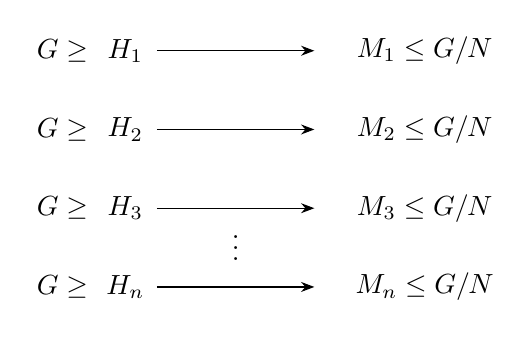
\begin{tikzpicture}
                \draw[->] (0,0) -- (2, 0);
                \draw[->] (0,-1) -- (2, -1);
                \draw[->] (0,-2) -- (2, -2);
                
                \node at (-0.4, 0) {$H_1$};
                \node at (-0.4, -1) {$H_2$};
                \node at (-0.4, -2) {$H_3$};
    
                \node at (3.4, 0) {$M_1 \le G/N$};
                \node at (3.4, -1) {$M_2 \le G/N$};
                \node at (3.4, -2) {$M_3 \le G/N$};

                \node at (-1.2, 0) {$G \ge $};
                \node at (-1.2, -1) {$G \ge $};
                \node at (-1.2, -2) {$G \ge $};
    
                \node at (1, -2.4) {$\vdots$};

                \node at (-0.4, -3) {$H_n$};
                \node at (3.4, -3) {$M_n \le G/N$};
                \node at (-1.2, -3) {$G \ge $};
                \draw[->] (0,-3) -- (2, -3);
                
            \end{tikzpicture}
        % \end{figure}
    \end{minipage}\hfill
    \begin{minipage}{0.55\textwidth}
        The Fourth Isomorphism Theorem is also commonly known as the
        correspondence theorem, since what it effectively states is that
        there is a one-to-one correspondence between subgroups $H$ of $G$
        which contain $N$ and the subgroups of $G/N$.

        Thus, if $G$ has $n$ subgroups $H_i$ which contain $N$, then $G/N$
        has $n$ subgroups.
    \end{minipage}


    \begin{prf}
        We first prove the first statement.

        \textcolor{NavyBlue}{Our goal here will be to show that $M \le
        G/N \implies M = H/N$ where $M$ is some subgroup of $G/N$ and
        $N \le H \le G$.} 
        \begin{description}
            \item[\phantom{1}]
            \hspace{0.5cm} Consider a subgroup $M$
            of $G/N$. Let $H$ be the set of all $h \in G$ such that
            $Nh \in M$. Then observe that $N \subset H$, since the smallest
            subgroup of $G/N$ is the trivial group, namely $\{N\}$.
            Therefore $N \subset H \subset G$.
            
            \textcolor{NavyBlue}{Now we
            show that $N \le H \le G$. To do this, we just need to
            show that $H \le G$, which we will do by the subgroup test.}

            Let $h, h' \in H$. Since $M \le G/N$, we know that for any
            $Nh, Nh' \in M$,  
            \[
                \underbrace{(Nh')(Nh)^{-1} \in M}_{\text{by the Subgroup Test}} \implies (Nh')(Nh^{-1}) \in M 
                \implies N(h'h^{-1}) \in M.
            \]
            However, in order for $N(h' h^{-1}) \in M$, we have that
            $h'h^{-1} \in H$. Since $h, h'$ were arbitrary elements of
           $H$, we have by the subgroup test we have that
            $H \le G$.  
            
            But since we have that $N \le G$, $H \le G$ and $N \subset
            H \subset G$, we all together have that $N \le H \le G$. 
        \end{description}
        Next, we prove the the statements $(1)-(4).$
        \textcolor{NavyBlue}{To prove (1), we'll show that $H/N \le K/N \implies H \le K$
        and $H \le K \implies H/N \le K/N$ for any subgroups $H, K$ of
        $G$ which contain $N$ where $N \normal G$.}

        \begin{description}
            \item[\phantom{1}]
            \hspace{0.5cm} Let $H, K$ be subgroups of $G$ such that $N
            \subset H$ and $N \subset K$. Furthermore, suppose that 
            $H/N \le K/N$.
            
        \end{description}
    \end{prf}

    
    The Isomophism Theorems are extremely powerful. The following
    an application to something which matches our intuiton, but
    extremely difficult to prove without the isomophism theorems.    
    \begin{thm}\label{product_theorem}
        Let $G$ be a group and $H$ and $K$ be normal subgroups of $G$.
        Then 
        \begin{itemize}
            \item[1.] $HK$ is a subgroup of $G$ 
            \item[2.] If $\gcd(|H|, |K|) = 1$ then $H \times K \cong
            HK$. 
        \end{itemize}
    \end{thm}

    \begin{prf}
        \begin{itemize}
            \item[1.] Observe that since $H \unlhd G$ and $K \unlhd G$, then obviously 
            $H \le G$ and hence we can apply the Second Isomorphism Theorem to conclude 
            that $HK \le G$. Thus we see that for this statement to be true in general 
            we really only need one of the subgroups, either $H$ or $K$, to be normal 
            to $G$.

            \textcolor{NavyBlue}{To prove this, we'll construct an
            isomorphism between the two groups. In constructing the
            homomorphism, we'll have to do a bit of work to show our
            proposed homorphism is in fact a homomorphism, the work
            which lies in showing elements of $H$ and $K$ commute.
            Thus we will show this first.}

            \item[2.]The fact that $\gcd(|H|,|K|)=1$ allows us to concldue that neither 
            $H \not \le K$ and $K \not \le H$, since otherwise by Lagrange's theorem 
            the order of one group would divide the other, and obviously we don't have 
            that case here. Thus we know that $H \cap K = \{e\}$, as by our previous 
            argument it would be impossible for them to share any other nontrivial element.
            \\
            \\
            Since $H, K$ are 
            normal to $G$ we'll have that 
            \begin{align*}
                hkh^{-1} \in K\\
                kh^{-1}k^{-1} \in H
            \end{align*}
            because $h$ and $k$ are both elements in $G$, and we know 
            for all $a \in G$ that $aha^{-1} \in H$ for $h \in H$ and 
            $aka^{-1} \in K$ for $k \in K$.
            We can then state that 
            \begin{align*}
                \overbrace{(hkh^{-1})}^{\text{A member of }K} \hspace{-0.3cm}k^{-1} = hkh^{-1}k^{-1} \in K\\
                h\underbrace{(kh^{-1}k^{-1})}_{\text{A member of } H} = hkh^{-1}k^{-1} \in H
            \end{align*}
            by using the fact that $H, K$ are subgroups and are therefore closed under products 
            of their elements. But we showed earlier that $H \cap K = \{e\}$; hence 
            $$
            hkh^{-1}k^{-1} \in H \cap K = \{e\} \implies hkh^{-1}k^{-1} = e \implies hk = kh.
            $$
            But $h, k$ were arbitrary elements of $H, K$, so this shows that products of 
            their elements commute.
            \\
            \\
            Next, consider the function $\phi: H \times K \rightarrow
            HK$ defined as
            $$
            \phi((h, k)) = hk.
            $$
            which we will 
            show to be a homomorphism.
            Observe that if $(h_1, k_1)$ and $(h_2, k_2)$ are in $H \times K$, then 
            $$
            \phi((h_1, k_1)\cdot(h_2, k_2)) = \phi((h_1h_2, k_1k_2)) = h_1h_2k_1k_2.
            $$
            However, we showed that products of elements between $H$ and $K$ can commute, so that 
            we can rewrite $h_2k_1$ as $k_1h_2$ to write 
            $$
            \phi((h_1, k_1)\cdot(h_2, k_2)) =  h_1h_2k_1k_2
            = h_1k_1h_2k_2 = \phi((h_1, k_2))\phi((h_2, k_2)).
            $$
            Thus $\phi$ is a homomorphism. \\
            \\
            Observe now that $\text{ker}(\phi) = \{(e, e)\}$. This is because we 
            know that $H \cap K = \{e\}$, so that if 
            $$
            \phi((h, k)) = hk = e
            $$
            we know it is impossible that this could be because $h = k^{-1}$; otherwise, 
            $H \cap K \ne \{e\}$, which we know is not the case. 
            Hence the only time when $hk = e$ is if both $h$ and $k$ 
            are $e$, so that $\text{ker}(\phi) = \{(e, e)\}$.
            \\
            \\
            Observe that $\text{im}(\phi) = HK$. This is because for any $hk \in 
            HK$, we can simply observe that $h \in H, k \in K$, and therefore there 
            exists a $(h, k) \in H \times K$ such that 
            $$
            \phi(h, k) = hk.
            $$
            Thus every element of $HK$ is covered by our mapping, so $\phi$ is injective 
            and hence $\text{im}(\phi) = HK$.
            \\
            \\
            Finally, what we have shown is that (1) $\phi$ is a homomorphism and 
            (2) it is a bijection from $H \times K$ to $HK$. We can now apply the 
            First Isomorphism Theorem to conclude that 
            $$ 
            H \times K/\text{ker}(\phi) \cong \text{im}(\phi) \implies H\times K \cong HK
            $$
            because $\text{ker}(\phi) = \{(e, e)\}, H \times K/\{(e, e)\} = H \times K$, 
            and $\text{im}(\phi) = HK$. This completes the proof.
        \end{itemize}
    \end{prf}

    The First Isomophism Theorem has a lot of fun applications, one of
    which we present here. 

    \begin{thm}
        Let $G$ and $H$ be groups such that $|G|$ and $|H|$ are
        coprime. If $\phi: G \to H$ is a homomorphism, then $\phi$ is
        zero homomorphism. 
    \end{thm}

    \begin{prf}
        By the First Isomorphism Theorem, we see that 
        \[
            G/\ker(\phi) \cong \im(\phi).   
        \]
        Therefore $|G/\ker(\phi)| = |\im(\phi)|$. However, 
        \begin{align*}
            |G/\ker(\phi)| = |G|/|\ker(\phi)| &= |\im(\phi)|\\ 
            \implies |G| &= |\ker(\phi)| \cdot  |\im(\phi)|.
        \end{align*}
        Note that $|\ker(\phi)| \mid |G|$ and $|\im(\phi)| \mid |H|$ by
        Lagrange's Theorem. However, we said that $|G|$ and $|H|$ are
        corpime
        which means that $|\im(\phi)| = 1$. Hence we
        must have that $|\ker(\phi)| = G$, and since $\ker(\phi) \le G$ we
        have that $\ker(\phi) = G$. Therefore $\phi$ sends every element
        of $G$ to the identity of $H$, which is what we set out to show.
    \end{prf}


    \newpage
    \section{Group Actions.}
    As we shall see, a group action is a special type of mapping one can
    formulate involving a group $G$ and an arbitrary set of objects $X$.
    Specifically, it is a mapping from $G \times X \to X$.
    Thus, a group action is said to make a group $G$ "act" on a set
    $X$. It is through this perspective that one can then view group
    actions as permutations of a set $X$. This becomes more clear with
    the formal definition. 

    \begin{definition}
        Let $G$ be a group and $X$ an arbitrary set. A \textbf{group
        action} of $G$ on $X$ is a mapping $* : G \times X \to X$
        that 
        \begin{itemize}
            \item[1.] $g_1 * (g_2 * x) = (g_1 \cdot g_2) * x$ for
            all $g_1, g_2 \in G, x \in X$.

            \item[2.] $e * x = x$ where $e \in G$ is the identity.
        \end{itemize}
    \end{definition}
    Note that $\cdot$ is the \textit{group multiplication in $G$.} For
    notational convenience, we will surpress $\cdot$ in the cases for
    where it's obvious or implied, as usual.
    \\
    We also note that we could have defined $*:X \times G \to X$. For
    simplicity, we let $G$ act on the left.
    \\  

    Let's breakdown what this is really saying.
    \textcolor{red}{For a group
    action $*$ of $G$ acting on $X$, we have for all $g \in G$, $x \in
    X$, the product $g * x$ is mapped to some element $x' \in X$.}

    Now observe that if
    we replaced $X$ with $G$, then we get $* : G \times G \to G$.
    Thus $*$ would just permutate the elements of $G$.
    Furthermore, if we let $*$ be the group multiplication $\cdot$ which
    is already defined in $G$, then we just get back the definition of
    a group! 
    
    \textcolor{NavyBlue}{This fits with the intuition that,
    group multiplication of elements (e.g., $g \cdot g'$ where $g, g'
    \in G$) simply permutates the elements of a group. That is, if 
    you placed the elements of $G$ in a tuple such as 
    \[
        (g_1, g_2, \dots, g_n)
    \] 
    and multiplied this by some $g' \in G$, you would get a tuple 
    \[
        (g_1, g_2, \dots, g_n) \cdot g' 
        = (g_1\cdot g', g_2 \cdot g' , \dots, g_n\cdot g')
        =
        (g_i, g_j, \dots, g_k)
    \]
    containing all the elements of $G$, but just in a different order.
    (In this case we supposed $g_1 \cdot g' = g_i, g_2, \cdot g' =
    g_j$, and so on.)
    } 

    \begin{minipage}{0.7\textwidth}
        \vspace{.3cm}
        This permutation phenonmenon can be found in more general
        group actions.  For a fixed $g \in G$, define $\sigma_g:
        X \to X$ as 
        \[
            \sigma_g(x) = g * x.
        \] 
        So $\sigma_g$ maps each $x$ to some other element $x' \in X$.
        Therefore, a group action can be thought of as a set of maps
        $\sigma_g$, one for every element $g \in G$, each of which can
        appropriately be composed with one another. 
        
        That's why
        it can be thought of as a permutation. The diagram on the right
        gives an illustration how this plays out for one particular
        $g \in G$ acting on a set $X$ with five elements.
    \end{minipage}\hfill
   \begin{minipage}{0.2\textwidth}
        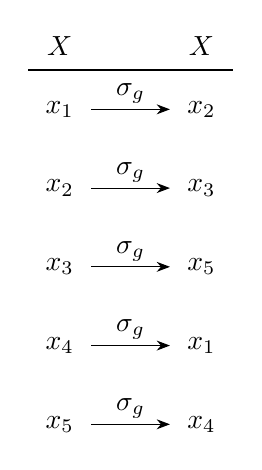
\begin{tikzpicture}
            \draw (-0.8,0.5)--(1.8,0.5);
            \draw[->] (0,0) -- (1,0);
            \draw[->] (0,-1) -- (1,-1);
            \draw[->] (0,-2) -- (1,-2);
            \draw[->] (0,-3) -- (1,-3);
            \draw[->] (0,-4) -- (1,-4);

            \node at (-0.4, .8) {$X$};
            \node at (-0.4, 0) {$x_1$};
            \node at (-0.4, -1) {$x_2$};
            \node at (-0.4, -2) {$x_3$};
            \node at (-0.4, -3) {$x_4$};
            \node at (-0.4, -4) {$x_5$};

            \node at (0.5, 0.2) {$\sigma_g$};
            \node at (0.5, -0.8) {$\sigma_g$};
            \node at (0.5, -1.8) {$\sigma_g$};
            \node at (0.5, -2.8) {$\sigma_g$};
            \node at (0.5, -3.8) {$\sigma_g$};
            
            \node at (1.4, 0.8){$X$};
            \node at (1.4, 0) {$x_2$};
            \node at (1.4, -1) {$x_3$};
            \node at (1.4, -2) {$x_5$};
            \node at (1.4, -3) {$x_1$};
            \node at (1.4, -4) {$x_4$};
            
        \end{tikzpicture}
        
    \end{minipage} 
    \vspace{.5cm}

    \textcolor{NavyBlue}{Here's another way to think about a group
    action. If $G$ acts on $X$, then the group action $*$ turns each 
    and every element of $g \in G$ into a \textit{function}, which
    maps $X$ to $X$. This agrees with our intuition, since a
    permutation is exactly a function of $X$ to itself. }
    \begin{thm}
        A finite group of order $n$ is isomorphic to a subgroup of $S_n$.
    \end{thm}
    
    This theorem is a powerful theorem that gives us a new way to
    think about finite groups. It states that every finite group is
    basically the same as a subgroup of a symmetric group up to an
    isomorphism. 

    \begin{prf}
        \textcolor{NavyBlue}{To prove this, we'll first construct a
        group action of $G$ on itself. Then we'll }

        Consider the group action of $G$ acting on itself, whereby we
        define $g_1 \cdot g_2 = g_1g_2$ for $g_1, g_2 \in G$. That is,
        the group action 
        mapping is simply the multiplication used between the elements
        of $G$. 
        \begin{description}
            \item[This is a Group Action.] 
            (Note: we already pointed out that if we replace $X$ with
            $G$ in the definition of a group action, and let $\cdot$
            be the group multiplication in $G$, then we just get the
            definition of a group. Thus a group is a special, but
            boring, type group action.)

            To show this is a group action, let $x \in G$. Then 
            \[
                g_1 \cdot (g_2 \cdot x) = g_1 \cdot (g_2x) = g_1g_2x = (g_1g_2)x = (g_1g_2) \cdot x.
            \]
            for $g_1, g_2 \in G$.
            Therefore, $g_1 \cdot (g_2 \cdot x) = (g_1g_2) \cdot x.$
            The second axiom is satisfied, since if $e$ is the
            identity of $G$, then clearly $e \cdot x = ex = x$. We
            have both axioms satisfied. So this is a group action. 
        \end{description}
    \end{prf}

    Before we lead up to a powerful theorem involving group actions,
    we must define a few definitions. 
    
    \begin{definition}
        Suppoe $G$ acts on a set $X$, and let $x \in X$. Then we
        define the set 
        \[
            Gx = \{g * x \mid g \in G \}
        \]
        as the \textbf{orbirt} of $x$. 
    \end{definition}

    The orbit basically considers the set of all images one obtains
    when one grabs a single element of $x \in X$, and multiplies it by
    every element $g \in G$. {\color{purple}{Note that since $g
    \cdot x \in X$ for every $g \in G, x \in X$, we have that $Gx \subset X$.}}
    
    \textcolor{NavyBlue}{Orbits are rather interesting since \textbf{they partition their acting
    set $X$}. That is, if $X = \{x_1, x_2, \dots, x_n\}$, then 
    $Gx_1 \cup Gx_2 \cup \cdots \cup Gx_n = X$. Note that $x_i \in
    Gx_i$ for $i = 1, 2, \dots, n$, so this definitely makes sense.
    \\
    \\
    However, it is possible that $Gx_i = Gx_j$ for some $i, j.$ In
    such a case we note that for each $g \in G$ there exists a $g' \in
    G$ such that $gx_i = g'x_j \implies g^{-1}g'x_j = x_i$. Since
    $g^{-1}g' \in G$, 
    our condition boils down to the following: 
    $Gx_i = Gx_j$ for some $i, j$ if there exists a $g \in G$
    such that 
    $gx_j = x_i$. So $Gx_i = Gx_j$ if $x_j \in Gx_i$.}
    \\
    \\
    Thus, these things are behaving like cosets (recall that $Gh =
    Gh'$ if and only if $h' \in Gh$.) and they partition the acting
    set $X$! This understanding will become helpful in the future. 
    \\
    \\
    Since orbits form partitions, and it is possible that the set of
    all orbits will be redundant (i.e., it's possible that $Gx_i =
    Gx_j$ for some $i, j$), we offer the following definition.

    \begin{definition}
        Let $G$ be a group, and suppose it acts on a set $X$. 
        Let $Gx_1, Gx_2, \cdots, Gx_n$ be a distinct set of
        orbits  such that 
        \[
            Gx_1 \cup Gx_2 \cup \cdots G_n = X.
        \]
        Then each $x_1, x_2, \dots, x_n$ are called
        \textbf{representatives of an orbit} of $G$. We generally
        denote $R = \{x_1, x_2, \dots x_n\}$ to be the set of
        representatives of the orbits. 
    \end{definition}

    Thus for some orbit $Gx_i$, we say that $x_i$ "represents" this
    orbit. We make this definition since we just showed that 
    it doesn't really matter what representative we pick, since if 
    $x_j \in Gx_j$, $Gx_j = Gx_i$, so $x_j$ could have equally
    represented this orbit. Thus given this arbitrary-ness, the
    definition allows us to talk about orbits more easily.
    
    We now offer another definition regarding group actions.

    \begin{definition}
        Suppose $G$ acts on $X$, and $x \in X$. Then the set 
        \[
            G_x = \{g \in G \mid g * x = x\}.
        \]
        is defined to be the \textbf{stabilizer} of $x$.
    \end{definition}
    
    The stabilizer considers the elements of $g \in G$ which act as an
    identity to $x$. \textcolor{purple}{Since $G_x$ considers elements
    of $G$, we see that $G_x \subset G$. Furthermore, we have the
    following proposition.}

    \begin{proposition}
        Suppose $G$ acts on $X$, and let $x \in X$. Then $G_x \le G$.
    \end{proposition}

    \begin{prf}
        Observe first that this is nonempty, since $e * x = x$ for
        all $x \in X$, where $e \in G$ is the identity. Therefore $e
        \in G_x$. Next, observe that associativity is inherited from
        the set $G$ itself. To check for inverses, we note that for any $g \in G$, $g \cdot x = x$, 
        so we can multiply both sides by $g^{-1}$ to get
        \[  
            g^{-1} * g * x = g^{-1} * x \implies (g^{-1}g) * x = g^{-1} * x 
            \implies x = g^{-1} * x.
        \]
        Thus $g^{-1} * x = x$ so $g^{-1} \in G$. Finally, observe
        that the set is closed. Given $g, g' \in G_x$, we see that 
        \[
            (gg') * x = g * (g' * x) = g *`' (x) = x.
        \]
        Therefore $G_x$ is (1) a subset of $G$ and (2) a group so it
        is a subgroup of $G$.

    \end{prf}
    We now move onto one of the useful theorems that arises once one
    realizes the definitions of the orbit and stabilizers.

    \begin{thm}
        Let $G$ be a finite group, and suppose $G$ acts on a set $X$.
        Then for any $x \in X$ we have that 
        \[
            |G| = |Gx| \cdot |G_x|.
        \]
    \end{thm}

    \begin{prf}
        To show this, we'll construct a bijection between $Gx$ and
        $G/G_x$. 

        Let $g \in G$ so that $gG_x \in G/G_x$. Then construct the map
        $\psi: G/G_x \to Gx$ by
        \[
            \psi(gG_x) = g * x.
        \]
        Note that there is only one element in $G/G_x$ which gets
       to $x$; namely, $G_x$. The calculation is as follows:
       \[
            \psi(G_x) = e * x = x.
       \]
       This map is obviously surjective, since for any $x' \in Gx$, we
        we know that there exists a $g \in G$ such that $g * x = x'$.
        Thus $g \not\in G_x$, so that $gG_x$ is nontrivial and
        $\psi(gG_x) = g * x = x'$.

        Now to show that this is injective, suppose that $g*x = h*x$.
     we have that $g^{-1}h * x = x$. Therefore, $gh^{-1} \in G_x$.
     Furthermoresee that 
     \[
         g^{-1}hG_x = G_x \implies hG_x = gG_x.
     \]
     Thus this can only happen if the input is the same. Therefore
     this is a one-to-one and onto mapping. 

     Since this is a bijection, we can conclude that 
     \[
        |Gx| = |G/G_x| = |G|/|G_x| \implies |G| = |Gx||G_x|    
     \]
     as desired.
    \end{prf}
    

    \newpage
    \section{Conjugation, The Class Equation, and Cauchy's Theorem.}
    \textcolor{blue}{We now touch on a very deep example of a group action, known as
    conjugation.} Let $G$ act on itself "by conjugation", which we define
    as follows. Let $g, h \in G$. Then 
    \[
        g * h = ghg^{-1}
    \]
    is the group action of conjugation.
    Let's show that this is a group action. 
    \begin{description}
        \item[Composition.] Let $g_1, g_2, h \in G$. Then observe that
        \begin{align*}
            g_1 * (g_2 * h) = g_1 * (g_2hg_2^{-1}) &= g_1g_2 h g_2^{-1}g_1^{-1} \\
            & = (g_1g_2) h (g_1g_2)^{-1} \\
            & = (g_1g_2) * h
        \end{align*}
        so that the first axiom of a group action is satisfied.
        \item[Identity.]
        Observe also that for $e \in G$, the identity of $G$, 
        \[
            e * h = ehe^{-1} = h.
        \]
        Therefore this is a group action.
    \end{description}

    We'll now show that this group action is very special and
    important. Conjugation itself is important in math. In Linear
    Algebra, two matrices which are similar (i.e., $A$ is similar to
    $B$ if there exists $P$ such that $A = P^{-1}BP$) have \textbf{the same 
    rank, determinants, trace, eigenvalues, and much more}. Basically,
    they represent the same linear transformation, just in different
    bases. To learn more about conjugation, we make a few definitions
    with this group action.

    \begin{definition}
        Let $G$ be a group, and let $G$ act on itself by conjugation.
        For any $h \in G$, \textbf{the orbit} of this group action
        \begin{align*}
            Gh & = \{g * h \mid g \in G\} \\
            & = \{ghg^{-1} \mid g \in G\}
        \end{align*}
        is known as a \textbf{conjugacy class} of $G$.
    \end{definition}

    \textcolor{purple}{Previously we discussed how orbits of a group action partition the
    set $X$ which is being acted on. Since $G$ acts on itself in this
    example, we see that \textbf{the conjugacy classes form a
    partition of $G$!}}
    \\
    \\
    \textbf{Remark.}
    Recall the definition of a centralizer $G$ for a set $A \subset
    G$: 
    \begin{align*}
        C_G(A) & = \{g \in G \mid gs = sg \text{ for all } s \in S\}\\
        & = \{g \in G \mid gsg^{-1} = s  \text{ for all } s \in S\}.
    \end{align*}
    Therefore for a single point $x \in G$, $C_G(x) = \{g \in G \mid
    gxg^{-1} = x \} = \{g \in G \mid g * x = x\}$, where in the last
    equation we are speaking in terms of group actions. But note that
    this last set is exactly the \textbf{stabilizer} of $G$ under this
    group action. \textbf{\textcolor{NavyBlue}{Therefore, $C_G(x) = G_x$ for any $x \in G$ under
    this group action.}}

    Furthermore, let $x \in Z(G) = \{z \in G \mid z = gzg^{-1} \text{
    for all } g \in G\},$ the center of $G$. Then we see that $Gx =
    \{gxg^{-1} \mid g \in G\} = \{x\}$. \textbf{\textcolor{NavyBlue}{So for any $x \in Z(G)$, the
    orbit is of size one. The sole element it contains is just $x$.}} (We can go even further: the conjugacy
    classes of an abelian group are all of size one.)
    \\
    \\
    Let's put all of these results together. In general, if $G$
    acts on itself via conjugation, then we know its orbits, or
    conjugacy classes, partition $G$. Moreover, let $R \subset X$ be a set of
    orbit representatives (or conjugacy class representatives, if you
    like). Then 
    \[
        |G| = \sum_{x \in R}|Gx|
    \]
    Recall that $|Gx| = 1$ if $x \in Z(G)$. Thus we can write this
    further as 
    \begin{align*}
        |G| = 
        \sum_{x \in Z(G)}|Gx| + \sum_{x \in R\setminus Z(G)} |Gx|
        & = \sum_{x \in Z(G)}1 + \sum_{x \in R\setminus Z(G)} |Gx|\\
        & = |Z(G)| + \sum_{x \in R\setminus Z(G)} |Gx|
    \end{align*}
    By the Orbit-Stabilizer theorem, we can write $|Gx| = |G|/|G_x|$.
    Substituting this in, we get 
    \begin{align*}
        |G| &= |Z(G)| + \sum_{x \in R\setminus Z(G)} |G|/|G_x|
    \end{align*}
    and since $C_G(x) = G_x$,
    \begin{align*}
        |G| = |Z(G)| + \sum_{x \in R\setminus Z(G)} |G|/|C_G(x)|
    \end{align*}
    which is known as the \textbf{class equation.} This equation is
    pretty badass, as it gives us a way to understand the cardinality
    of a group. This equation is also useful in proofs, as we shall
    see in the following examples. First, we begin with a lemma. 

    \begin{lemma}
        Let $G$ be a group. Then $C_G(x) = G$ if and only if $x \in Z(G)$.
    \end{lemma}

    \begin{prf}
        Suppose $C_G(x) = G$. Then for all $g \in G$, $gx = xg$.
        However, $Z(G)$ is the set of all $G$ which commutes with
        every member of $G$, so $x \in Z(G)$. 
        Now suppose $x \in Z(G)$. Then $gx = xg$ for all $g \in G$.
        Therefore, $C_G(x) = \{g \in G \mid gx = xg\} = G$.
    \end{prf}

    \begin{thm} \label{center_lemma}
        Let $G$ be a group such that $|G| = p^n$ for some prime $p$
        and $n \in \mathbb{N}$. Then $|Z(G)| > 1$. That is, $|Z(G)|
        \in \{p, p^2, \dots, p^{n}\}$.
    \end{thm}
    \textcolor{Purple}{Equivalently, this theorem says that $Z(G)$ is nontrivial.
    Moreover, this implies that \textbf{there exists
    non identity elements of $\mathbf{G}$ which commute with every
    element of $\mathbf{G}$.}}

    \begin{prf}
        First observe that $Z(G)$ is a subgroup of $G$. Therefore, by
        Lagrange's Theorem, we know that $|Z(G)|$ divides $G$. Thus
        $|Z(G)| \in \{1, p, p^2, \dots, p^{n}\}$. Our goal is to show
        that $|Z(G)|$ cannot equal 1.

        \textcolor{NavyBlue}{For the sake of contradicton, suppose $|Z(G)| = 1$}. Then by
        the previous lemma, we see that 
        there is no nontrivial element $g$ of $G$ such $C_G(g) = G$.

        Let $R$ be the set of conjugacy class representatives. 
        Then $|G|/|C_G(r)| \in \{p, p^2, \cdots, p^n\}$ for $r \in
        R\setminus Z(G)$ (since $|Z(G)| = 1$, $R\setminus Z(G)$ simply
        removes $e$, the identtiy, from $R$).

        \textcolor{red!40!purple!100}{Why can't $|G|/|C_G(r)| = 1$ for any $r \in
        R\setminus Z(G)$? Well, because for such an $r$, $r \not\in
        Z(G)$. Therefore $C_G(r) \ne G$, so $|G|/|C_G(r)| \ne 1$.}

        Now by the class equation, we see that 
        \[
            \underbrace{ \hspace{.2cm}|G|\hspace{.2cm}   }_{\text{divisible by } p} \hspace{-.5cm} = |Z(G)| + \overbrace{\sum_{r \in R\setminus Z(G)} |G|/|C_G(r)|}^{\text{divisible by } p}
        \]
        since $|G|/|C_G(r)| \in \{p, p^2, \dots, p^n\}$ for all $r \in
        R\setminus Z(G)$. \textcolor{NavyBlue}{Therefore we see that $|Z(G)|$ must be
        divisible by $p$. But this is a contradiction since we said
        $|Z(G)| = 1$}. Therefore, we see that $|Z(G)| \in \{p, p^2,
        \dots, p^n\}$.
        
    \end{prf}

    The above theorem can be used to prove the next theorem, whose
    signifiance demonstrates the power of the class equation.
    The theorem below is generally
        proved by proving the above theorem first in the special case
        for when $|G| = p^2$. But it will be helpful to other proofs
        later on to consider the more general case as we presented it above.

    \begin{thm}
        Let $G$ be a group, and suppose $|G| = p^2$ where $p \ge 2$ is
        prime. Then $G$ is abelian. 
    \end{thm}

    \begin{prf}
        \textcolor{green!50!black}{By the previous theorem, we see
        that $|Z(G)| \in \{p, p^2\}$.)} We'll proceed by considering two cases.

        \begin{description}
            \item[$\mathbf{|Z(G)| = p^2}$.] 
            In this case $|G| = |Z(G)|$. Since we also have that
            $Z(G)$ is a subgroup of $G$, we can conclude that $G =
            Z(G)$. 
            Therefore, $G$ is abelian. 
             
            \item[$\mathbf{|Z(G)| = p}$.] 
            Recall that $Z(G) \normal
            G$ from Proposition \ref{normal_center}. Therefore, we can
            speak of the quotient group $G/Z(G)$, which has size
            $|G|/|Z(G)| = p^2/p = p$. By the corollary to Lagrange's
            Theorem, this implies that $G/Z(G)$ is cyclic, since it
            has prime order. Thus there
            exists a $g \in G$ such that we can represent $G/Z(G)$ as 
            \[
                G/Z(G) = \{Z(G), Z(G)g, Z(G)g^2, \dots, Z(G)g^{p-1}\}.
            \]
            As we already know, cosets partition $G$. Therefore, let
            $a, b \in G$, and suppose $a \in Z(G)g^i$ and $b \in
            Z(G)g^j$. Then there exist $x, y \in Z(G)$ such that 
            $a = xg^i$ and $b = yg^j$. Thus observe that 
            \begin{align*}
                ab = xg^i yg^j = xyg^ig^j = xyg^{i+j} = xyg^jg^i
                = yg^jxg^i = ba
            \end{align*}
            where we used the commutavity of $x,y$ since $x, y \in
            Z(G)$. Since $a, b$ were arbitrary members of $G$, this
            proves that $G$ is abelian.
        \end{description}
    \end{prf}

    Thus we see that the class equation is useful in proving more
    general facts about group theory. The class equation can also be
    used to prove the following important theorem in group theory,
    known as Cauchy's Theorem. 

    \begin{thm}[ (Cauchy's Theorem)]
        Let $G$ be a finite group and $p \ge 2$ be a prime. If $p$ divides
        the order of $G$, then $G$ has an element of order $p$. 
    \end{thm}

    \noindent\textcolor{NavyBlue}{So consider a group $G$ with order $n$,
    and suppose 
    \[ n = p_1^{i_1}\cdot p_2^{i_2} \cdots
    p_n^{i_n}
    \]
    is its prime factorization. Then there exist elements
    $g_1, g_2, \dots, g_n$ such that $|g_i| = p_i$ for $i = 1, 2,
    \dots, n$.}

    Another way to visualize this as follows. Consider a group $G$
    consisting of 10 elements. 
    \[
        \{e, \hspace{.1cm}g_1,\hspace{.1cm} g_2,\hspace{.1cm} g_3,\hspace{.1cm} g_4,\hspace{.1cm} g_5,\hspace{.1cm} g_6,\hspace{.1cm} g_7,\hspace{.1cm} g_8,\hspace{.1cm} g_{9}\}
    \]
    By Cauchy's theorem, there exists elements of order $2$ and $5$.
    So suppose $g_1$ and $g_2$ are such elements, i.e., $g_1^2 = 3$
    and $g_2^5 = e$. Then we can really rewrite this as 
    \[
        \{e,\hspace{.1cm} \textcolor{red}{g_1},\hspace{.1cm} \textcolor{blue}{g_2},\hspace{.1cm} \textcolor{blue}{g_2^2},\hspace{.1cm} \textcolor{blue}{g_2^3},\hspace{.1cm} \textcolor{blue}{g_2^4},\hspace{.1cm} g_6,\hspace{.1cm} g_7,\hspace{.1cm} g_8,\hspace{.1cm} g_9\}.   
    \] 
    However, we know $\textcolor{red}{g_1}\textcolor{blue}{g_2}, \textcolor{red}{g_1}\textcolor{blue}{g_2^2}, \textcolor{red}{g_1}\textcolor{blue}{g_2^3}$ and $\textcolor{red}{g_1}\textcolor{blue}{g_2^4}$ are all in $G$. Thus
    we can really write this as 
    \[
        \{e, \hspace{.1cm} \textcolor{red}{g_1},\hspace{.1cm} \textcolor{blue}{g_2},\hspace{.1cm} \textcolor{blue}{g_2^2},\hspace{.1cm} \textcolor{blue}{g_2^3},\hspace{.1cm} \textcolor{blue}{g_2^4}, \hspace{.1cm}\textcolor{red}{g_1}\textcolor{blue}{g_2},\hspace{.1cm} \textcolor{red}{g_1}\textcolor{blue}{g_2^2},\hspace{.1cm} \textcolor{red}{g_1}\textcolor{blue}{g_2^3},\hspace{.1cm} \textcolor{red}{g_1}\textcolor{blue}{g_2^4}\}.
    \] 
    Thus we can understand the structure of every single group of
    order 10. But this can be done for all finite groups!
    
    \begin{prf}
        \textcolor{Plum}{In this proof, we'll prove this in a very
        clevery way by letting a subgroup of a permutation group act
        on a special set $X$ (both of which we will define). This will then prove the existence of
        elements of order $p$.}

        Let $p$ be a prime which divides $|G|$. 
        Define $H$ to be the cyclic subgroup of $S_p$ generated by
        $(1\hspace{.1cm}2\hspace{.1cm}\cdots\hspace{.1cm}p)$. 

        We can picture $H$ as the group 
        \[
            \{(1\hspace{.1cm}2\hspace{.1cm}\cdots\hspace{.1cm}p), (2\hspace{.1cm}3\hspace{.1cm}\cdots\hspace{.1cm}p, \hspace{.1cm}1), \cdots, (p\hspace{.1cm}1\hspace{.1cm}\cdots\hspace{.1cm}p-1)\}.
        \]

        Now let $H$ act on the set $X$ defined as 
        \[
            X = \{ (g_1, g_2, \dots, g_p) \mid g_1, g_2, \dots, g_p \in G \text{ and } g_1g_2\cdots g_p = e \}
        \]
        where the $\sigma \in H$ acts on $g \in X$ as 
        \[
            \sigma \cdot (g_1, g_2, \dots, g_p) = (g_{\sigma(1)}, g_{\sigma(2)}, \dots, g_{\sigma(p)}).
        \]
        This $H$ takes a $p$-tuple in $X$ and permutates the elements.
        Since $H$ is generated by
        $(1\hspace{.1cm}2\hspace{.1cm}\cdots\hspace{.1cm}p)$, it
        "pushes" the elements $g_i$ in the tuple over to the right, and the elements
        that are pushed out of the right end of the tuple are pushed back in on
        the left side.

        \textcolor{NavyBlue}{First we'll show that this is a group action.}
        \begin{description}
            \item[This is a Group Action.] 
                Let $x \in X$ and $\sigma \in H$. If $x = (g_1, g_2,
                \dots , g_p)$, observe that 
                \[
                    \sigma * x = (g_{\sigma(1)}, g_{\sigma(2)}, \dots, g_{\sigma(p)}).
                \]
                Suppose $h(1) = n$. Then in general $h(i) = (i + n)
                \mbox{ mod }p.$ Therefore, we see that 
                \[
                    (g_{\sigma(1)}, g_{\sigma(2)}, \dots, g_{\sigma(p)}) 
                    = 
                    (g_{n}, g_{n+1}, \dots, g_p, g_1, \dots, g_{n-1}).
                \]
                However, observe that 
                \[
                    g_1g_2\cdots g_p = g_1g_2 \cdots g_{n-1}g_n g_{n+1} \cdots g_p = e
                    \implies (g_1g_2 \cdots g_{n-1})(g_n g_{n+1} \cdots g_p) = e.
                \]
                Thus the elements $g_1g_2 \cdots g_{n-1}$ and $g_n
                g_{n+1} \cdots g_p$ in $G$ are inverses of each other. But
                know that if two group elements are inverses, either order
                of their product returns $e$. Therefore 
                \[
                    (g_ng_{n+1} \cdots g_{p})(g_1g_2 \cdots g_{n-1}) 
                    = g_ng_{n+1} \cdots g_{p}g_1g_2 \cdots g_{n-1} = e.
                \]
                                
                We therefore see that
                $(g_{n}, g_{n+1}, \dots, g_p,
                g_1, \dots, g_{n-1}) = \sigma *x \in X$. 

                Now we verify associativity. For any $\sigma_1,
                \sigma_2 \in H$, we see that 
                \begin{align*}
                    \sigma_1 * \sigma_2*x &= \sigma_1 * (g_{\sigma_2(1)}, g_{\sigma_2(2)}, \dots, g_{\sigma_2(p)})\\
                    &= (g_{\sigma_1(\sigma_2(1))}, g_{\sigma_1(\sigma_2(2))}, \dots, g_{\sigma_1(\sigma_2(p))})\\
                    &= (\sigma_1 \sigma_2) * (g_1, g_2, \dots, g_p).
                \end{align*}
                Thus $*$ is associative. Finally, if $\sigma$ is the
                trivial element, 
                \[
                    \sigma * x = (g_{\sigma(1)}, g_{\sigma(2)}, \cdots g_{\sigma(p)}) = (g_1, g_2, \dots, g_p) = x.
                \]
                Therefore this is a group action.
        \end{description}
        \textcolor{NavyBlue}{Now that we've shown that this is a group
        action, we'll argue that the orbits are either of size 1 or
        $p$.}
        
        \begin{description}
            \item[The Orbits.] 
            For any $x \in X$ such that $x = (g_1, g_2, \dots, g_p)$,
            we see that the orbit $Hx$ will simply be all of
            the permutations of the $p$-tuple $(g_1, g_2, \dots,
            g_p)$. Note however that there are only $p$ many ways to
            rearrange this tuple, so that any orbit $Hx$ will be of
            size $p$.

            Of course, the exception to this is if $g_1 = g_2 = \dots = g_p$. In
            this case, there are no other ways to reorganize the
            tuple. Hence the orbit will have size 1.
        \end{description}

        \textcolor{NavyBlue}{Finally, we will show that there exists a
        nontrivial orbit of size 1. This is equivalent to show that
        there exists a nontrivial element of $G$ of order $p$, which
        we'll eloaborate later.}

        \begin{description}
            \item[Orbit of Size 1.]
            First let's count the elements of $X$. Observe that for
            any $(g_1, g_2, \dots, g_p) \in
            X$, the last element $g_p$ is always determined by the
            first $p-1$ elements. This is because if we know the first
            $p-1$ elements, then 
            \[
                g_p = (g_1g_2 \cdots g_{p-1})^{-1}
            \]
            in order for $g_1g_2\cdots g_p = e$. Since there are
            $|G|^{p-1}$ many ways to pick the first $p-1$ elements in
            any $p$-tuple of $X$, we see that $X = |G|^{p-1}$. 

            Now by hypothesis, $p$ divides $|G|$. Therefore $p$
            divides $|X|$ so we may write $|X| = np$ for some integer $n$.

            Since the orbits of $X$ form a partition, the orbits
            partition a set $np$ elements into orbits of size $1$ or
            size $p$. We know one orbit of size 1 exists (namely, the
            trivial orbit $He = \{(e, e, \dots, e)\}$), so there must
            exist at least $p-1$ nontrivial other orbits of size 1. 

            Let $Hx'$ be one of those orbits. Then for some $g \in G$
            we have that $Hx = \{(g, g, \dots, g)\}$. However since
            $Hx \subset G$, what we have prove is the existence of a
            nontrivial
            element $g \in G$ such that $gg\cdots g = g^p = e$, which
           set out to show.
        \end{description}
        This completes the proof.
    \end{prf}
    Cacuhy's Theorem is an incredibly useful tool one can use in
    finite group theory. Here's an amazing and useful theorem who's
    proof is eased via Cauchy's Theorem.

    \begin{thm}
        Let $G$ be a group $p \ge 2$ a prime. If $|G| = p^n$ for some
        $n \in \mathbb{N}$, then $G$ has a subgroup of order $p^k$ for
        all $0 < k < n$.
    \end{thm}
    Note we didn't write $ 0 \le k \le n$. We could have, but we already
        know that there exists a subgroup of order $p^n$ (namely, $G$
        itself) and that there exists a subgrou of order $p^0 = 1$
        (namely, the trivial group).
    \begin{prf}
        \textcolor{NavyBlue}{To prove this, we'll use strong induction
        on the statement. Specifically, we'll induct on the powers of
        $n$.}

        Let us induct on $n$ in the statement above. Then for $n = 1$,
        there is no such $k < n$. Hence the statement is vacuously
        true. 

        Next suppose that the statement is true up to order $p^n$, 
        and let $G$ be a group of order $p^{n+1}$. 

        By Theorem 1.\ref{center_lemma}, we already note that $|Z(G)| >
        1$ and hence is a multiple of $p$. By Cauchy's Theorem, we
        then know that $Z(G)$ contains an element $g$ of order $p$.
        Note that (1) $\left< g\right>$ is a subgroup of $Z(G)$ and
        (2) $h\left< g \right> = \left< g \right>h$ for all $h \in G$
        (since, by definition of the center, every element of $Z(G)$
        commutes with elements of $G$). Therefore $\left< g \right>
        \normal G$. 

        Let $H = \left< g \right>$. Since we just showed $H \normal G$
        we can appropriately discuss the quotient group $G/H$.

        Observe that $|G/H| = |G|/|H| = p^{n+1}/p = p^n$. \textcolor{purple}{Thus by hypothesis, $G/H$ has a
        subgroup of order $p^k$ for all $0 < k < n$. Denote these such
        subgroups of $G/H$ as}
        \[
            \{N_1/H, N_2/H, \cdots N_{n-1}/H\}
        \]
        \textcolor{purple}{where $|N_k/H| = p^k$.}
        Since $H \normal G$, we
        know by the Fourth Isomorphism Theorem that every subgroup of
        $G/H$ is of the form $N/H$ where $H \le N \le G$. Thus we see
        that 
        \[
            H \le N_k \le G
        \]
        for all $0 < k < n$. But since $|N_k/H| = p^k$, and $|H| = p$,
        we see that each such $N_k$ will now have order $p^{k+1}$.
        Thus what we have shown is that $G$ itself contains subgroups
        of order $k$ for all $1 < k < n+1$. The subgroup $H$ of order
        $p$ is the final piece to this puzzle, and allows us to
        confirm that $G$ has a subgroup of order $p^k$ for all $0 < k < n$.
        By strong induction this holds for all $\mathbb{N}$,
        which completes the proof.
    \end{prf}



    \newpage
    \section{Sylow Theorems.}
    Lagrange's Theorem states that $H \le G$, then $|H|$ divides
    $|G|$. However, you may wonder if there is some kind of converse.
    If $k$ divides $|G|$, is there a subgroup of order $k$? 

    By Cauchy's Theorem, we know that if $p$ is a prime which divides
    then there exists an element of order $p$. Can we generalize this
    result further (for example, state \textit{how} many such elements
    satisfy this)? 

    The answer to both questions is yes and is achieved through
    Sylow's Theorem. It's a foundational theorem in finite group
    theory, as it
    strengthens our two most power theorems for finite groups:
    Lagrange's Theorem and Cauchy's Theorem.

    \begin{definition}
        $H$ is a \textbf{$p$-subgroup} of a group $G$ if $H$ is a
        subgroup of $G$ and $|H| = p^n$ for some $n \ge 1$.
    \end{definition}

    \begin{definition}
        Let $G$ be a group and let $p$ be a prime such that $p\mid
        |G|$. Suppose $p^k$ is the largest power such that $p^k \mid
        |G|$. That is, $|G| = p^km$ for some integer $m \in G$,
        $\mbox{gcd}(p, m) = 1$. Then any subgroup $H$ of $G$ with $|H| = p^k$ is called a
        \textbf{Sylow $p$-subgroup}.
        \\
        \\
        An equivalent definition is the following: $H$ is a 
        \textbf{Sylow-$p$ subgroup} if $H$ is a $p$-subgroup where
        $|H| = p^k$.
    \end{definition}

    \textcolor{purple}{A Sylow $p$-subgroup is nothing more than a subgroup $H$ where
    $|H| = p^k$ and $|G| = p^km$ where $\mbox{gcd(p, m)} = 1$.}

    \begin{definition}
        Let $G$ be a group and $P$ and $Q$ be subgroups of $G$. If
        there exists an element $g \in G$ such that 
        \[
            gPg^{-1} = Q
        \]
        then $P$ is \textbf{conjugate} to $Q$.
    \end{definition}
    Recall that if $H \normal G$, then for any $g \in G$ we see that
    $gHg^{-1} = H$. Thus $H$ is conjugate to itself.
    Also note that if $P$ is a subgroup then so is $gPg^{-1}$.

    \begin{thm}[ (Sylow Theorem)] Let $G$ be a finite group and $p$ a
    prime such that $p \mid |G|$. Suppose further that $|G| = p^km$
    where $\mbox{gcd}(p, m) = 1$. Then 
    \begin{itemize}
        \item[1.] There exists a Sylow $p$-subgroup (equivalently, there
        exists a subgroup $H$ of $G$ where $H = p^k$) and every
        $p$-subgroup of $G$ is contained in some Sylow $p$-subgroup 

        \item[2.] All Sylow $p$-subgroups are conjugate to each other,
       and the conjugate of any Sylow $p$-subgroup is also a Sylow
       $p$-subgroup
       \item[3.] If $n_p$ is the number of Sylow $p$-subgroups, then 
       \[
           n_p \mid m \hspace{0.5cm}\text{and}\hspace{0.5cm} n_p = 1 \mbox{ mod } m.
       \] 
    \end{itemize}
    \vspace{-.4cm}
    \end{thm}

    \begin{prf}
        \textcolor{NavyBlue}{We can prove the first part by letting
        $G$ act on a special set $\Omega$. It will turn out that the
        stabilizer of our action will be the desired Sylow
        $p$-subgroup.}
        
        \begin{itemize}
            \item[1.] Define 
            \[
                \Omega = \{ X \subset G \mid |X| = p^k\}
            \] 
            and let $G$ act on $\Omega$ from the
            left. Observe that for $X \in \Omega$, $g * X = \{gx \mid
            \text{ for all } x \in X\} = gX.$ Since $|gX| = |X| = p^k$, we
            see that $gX \in \Omega$. Associativity and identity
            applications are trivial, so we get that this is a group
            action.
            
            \textcolor{NavyBlue}{Now that we have shown that this is a
            group action, we will consider the orbits of the group
            aciton.}
            
            Since $|G| = p^km$, there are $\displaystyle
            \binom{p^km}{p^k}$ many ways for us to choose a subset $X$
            of $G$ with size $p^k$. Hence $|\Omega| = \displaystyle
            \binom{p^km}{p^k}$. Note that since this is a group action, the
            orbits form a partition of $X$. Now from number theory, we
            know that 
            \[
                \binom{p^km}{p^k} = m \mbox{ mod } p.
            \]
            Since the orbits must partition $\Omega$, the above result
            tells us that we cannot partition $G$ with sets which are
            divisible by $p$. In other words, there must exist some
            orbit $\mathcal{O}$
            such that $|\mathcal{O}|$ is not divisible by $p$. 

            \textcolor{NavyBlue}{Now that we know that there exists an
            orbit not divisible by $p$, we will anaylze the
            corresponding stabilizer of this orbit. This stabilizer
            will turn out to be our Sylow $p$-subgroup. }

            Let $H$ be the orbit corresponding to $\mathcal{O}$. Then
            by the Orbit-Stabilizer Theorem 
            \[
                |G| = |\mathcal{O}||H| \implies p^km = |\mathcal{O}||H|.                
            \]
            By the last equation, we see that $p^k$ must divide both
            sides. However, $|\mathcal{O}|$ is not divisible by $p$.
            Hence $|H|$ must be divisible by $p^k$.
            
            However, by Lagrange's Theorem, $|H|$ divides $|G| =
            p^km$. Therefore $|H| = m$ or $|H| \in \{1, p, p^2, \dots,
            p^k\}$. In either case $|H| \le p^k$ (since $m \le p$).
            But we just showed that $p^k$ divides $|H|$, which proves
            that $|H| = p^k$. 
            
            Since $H$ is a stabilizer, $H \le G$, so
            we have effectively proved the existence of a subgroup of
            order $p^k$; or, in other words, a Sylow $p$-subgroup. 

        \item[2.]
            Suppose $H$ and $K$ are Sylow $p$-subgroups of $G$. 
            Then observe that 

        \item[3.] 
            


            
        \end{itemize}
    \end{prf}

    The consequences of this theorem are immediate. 
    \begin{proposition}\label{sylow_normal}
        Let $G$ be a finite group and suppose $|G| = p^km$ for some
        prime $p$ where $\mbox{gcd}(p, m) = 1$. Then $G$ has a normal
        subgroup of order $p^k$ if and only if $n_p = 1$.
    \end{proposition}

    \begin{prf}
        ($\implies$) Suppose $G$ has a normal subgroup $H$ of order $p^k$. By
        Sylow's Theorem, we know that all 
        other Sylow $p$-subgroups are conjugate to $H$. Thus let $g
        \in G$ and observe that 
        \[
            gHg^{-1} = H
        \]
        since $H$ is normal. Therefore, there are no other Sylow
        $p$-subgroups so $n_p = 1.$
        
        ($\impliedby$) Now suppose that $n_p = 1$. Let $H$ be a sole
        Sylow $p$-subgroup of $G$. Since it is the only Sylow
        $p$-subgroup, we see that 
        \[
            gHg^{-1} = H
        \]
         for all $g \in G$. However this exactly the definition for
         $H$ to be a normal subgroup of $G$. This proves the result.
    \end{prf}

    Once you use Sylow's Theorem and study finite groups more, you'll
    realize that some groups aren't that complicated. For example,
    consider \textit{any} subgroup of order 4. This can be any wild
    group you want, but at the end of the day, it turns out one of the
    following options is true:
    \[
        G \cong \mathbb{Z}/4\mathbb{Z} \hspace{0.2cm}\text{ or }\hspace{.2cm} 
        G \cong \mathbb{Z}/2\mathbb{Z} \times \mathbb{Z}/2\mathbb{Z}.
    \]
    The process leading to such a conclusion is known as
    \textbf{classifying groups up to an isomorphism}. That is, you
    start with a group with a fixed order, and then determine much
    simpler groups that your group could be isomorphic to. In our
    example, we say that any group of order 4 can only be two things
    up to an isomorphism.
     
    The cool thing about Sylow's Theorem is that it is so strong that
    it allows us to classify groups up to an isomorphism. 

    In general, when classifying groups up to an isomorphism, it is
    convenient to do in terms of integer groups $\mathbb{Z}$ or
    modulo integer groups, as we saw above. This isn't always
    possible, but when it is, the following theorem comes in handy.

    \begin{thm} \label{zmod_iso_thm}
        Let $m, n$ be positive integers. Then 
        \[
            \mathbb{Z}/mn\mathbb{Z} \cong \mathbb{Z}/m\mathbb{Z} \times \mathbb{Z}/n\mathbb{Z}
        \]
        if and only if $m$ and $n$ are coprime.
    \end{thm}


    \noindent
    \textbf{Example.}
    \\
    \textcolor{NavyBlue}{Suppose we want to classify all groups of order 1225 up to an
    isomorphism.}
    \\
    Let $G$ be a group such that $|G| = 1225 = 5^27^2$. Then observe
    $\mbox{gcd}(5, 7^2) = 1$. By Sylow's theorem, we know that 
    if $n_5$ is the number of Sylow $5$-subgroups of $G$, then 
    \[
        n_5 \big| 7^2 \quad \text{ and }\quad n_5 \equiv 1 \mbox{ mod } 5.
    \]
    Observe that $n_5$ can only equal 1. Since $n_5 = 1$, we know by
    Propsition \ref{sylow_normal} that
    for the unique Sylow 5-subgroup $H$ that $H \unlhd G$. Also note
    that $|H| = 5^2$.
    \\
    \\
    Now observe that $\mbox{gcd}(7, 5^2) = 1$. By Sylow's Theorem, we
    know that if $n_7$ is the number of Sylow 7-subgroups of $G$ that 
    \[
       n_7 \big| 5^2 \quad \text{ and }\quad n_7 \equiv 1 \mbox{ mod } 7.
    \]
    Note that $n_7$ must also equal 1. Thus again for the unique Sylow
    7-subgroup $K$, we must have that $K \unlhd G$ and $|K| = 7^2$. Now we can observe
    that (1) $\mbox{gcd}(|H|, |K|) = 1$ and (2) $|G| = |H||K|$ so that
    \[
        G \cong H \times K     
    \]
    by Theorem 1.\ref{product_theorem}. 
    Now observe that since $|H| = 5^2$, $H \cong
    \mathbb{Z}/25\mathbb{Z}$ and $H \cong \mathbb{Z}/5\mathbb{Z}
    \times \mathbb{Z}/5\mathbb{Z}$. Since $K = 7^2$, $K \cong 
    \mathbb{Z}/49\mathbb{Z}$ and $H \cong (\mathbb{Z}/7\mathbb{Z}
    \times \mathbb{Z}/7\mathbb{Z})$.
    Therefore, we see that the groups of order 1225 are, up to
    isomorphism, 
    \begin{itemize}
        \item[(1)] $(\mathbb{Z}/25\mathbb{Z}) \times (\mathbb{Z}/49\mathbb{Z})$
        \item[(2)] $(\mathbb{Z}/25\mathbb{Z}) \times
        (\mathbb{Z}/7\mathbb{Z} \times \mathbb{Z}/7\mathbb{Z})$
        \item[(3)] $(\mathbb{Z}/5\mathbb{Z} \times \mathbb{Z}/5\mathbb{Z})
        \times \mathbb{Z}/49\mathbb{Z}$
        \item[(4)] $(\mathbb{Z}/5\mathbb{Z} \times \mathbb{Z}/5\mathbb{Z})
        \times (\mathbb{Z}/7\mathbb{Z} \times
        \mathbb{Z}/7\mathbb{Z})$.
    \end{itemize}
    \textcolor{purple}{We suspect that these are all the groups of
    order 1225 up to an isomorphism. However, we double check that
    none of these groups are actually equivalent to each other, i.e.,
    that we have no redundancies.}

    Observe that (1)
    is not isomorphic to any of the the other groups, since $(1, 1)
    \in (\mathbb{Z}/25\mathbb{Z}) \times (\mathbb{Z}/49\mathbb{Z})$,
    has order 1225 but none of the other groups have an element of
    order 1225.
    \\
    \\
    In addition, (3) is not isomorphic to (2) or (3) since $(0, 1) \in
    (\mathbb{Z}/5\mathbb{Z} \times \mathbb{Z}/5\mathbb{Z})
        \times \mathbb{Z}/49\mathbb{Z}$ and has
    order 49
    but no element of either (2) or (3) has an element of either 49. 
    \\
    \\
    Finally, we see that (2) is not isomorphic to (4) because $(1, 0)
    \in (\mathbb{Z}/25\mathbb{Z}) \times
    (\mathbb{Z}/7\mathbb{Z} \times \mathbb{Z}/7\mathbb{Z})$ is an
    element of order 25 but there is no element of order 25 in (4).
    Thus we see that (1) these subgroups are isomorphic to $G$ and (2)
    none of them are isomorphic to each other. Therefore, this an
    exhaustive list of all the groups of order 1225 up to isomorphism.

    Here's another example in which Sylow's Theorem helps us classify
    a specific type of group.

    \begin{thm}
        Let $p,q$ be primes with $p<q$ and suppose $p$ does not divide
        $q-1$.  If $G$ is a group such that $|G| = pq$, then 
        $G \cong \mathbb{Z}/pq\mathbb{Z}$. 
    \end{thm}

    \begin{prf}
        Let $G$ be a group and $|G| = pq$. Since $\mbox{gcd}(p, q) = 1,$
        by the Sylow Theorem, 
        there exists a Sylow $p$-subgroup and Sylow $q$-subgroup of $G$. 
        \\
        Now let $n_p$ and $n_q$ be the number of Sylow $p$ and $q$-subgroups,
        respectively. Then observe that 
        \[
          n_p \big|q \qquad n_p \equiv 1 \mbox{ mod } p   
        \]
        so that $n_p = 1$ and 
        \[
            n_q \big|p   \qquad n_q \equiv 1 \mbox{ mod } q.
        \]
        Now observe that $n_p = 1$ or $q$. However, since $p$ does not divide
        $q - 1$, we know that 
        \[
          q \not\equiv 1 \mbox{ mod } p.  
        \]
        Thus $n_p = 1$. Again, either $n_p = 1$ or $p$ but $p < q$ so 
        \[
           n_q \not\equiv 1 \mbox{ mod } q 
        \]
        unless $n_q = 1$. Thus there is one and only one Sylow $p$-subgroup
        and Sylow $q$-subgroup, which we can call $H$ and $K$ respectively.
        By proposition \ref{sylow_normal}, 
        \[
          H \unlhd G \qquad K \unlhd G.  
        \]
        Note that (1)
        $\mbox{gcd}(|H|, |K|) = \mbox{gcd}(p, q) = 1$ and (2) $|G| = |H||K| =
        pq$. Thus $G \cong H \times K$ by Theorem 1.\ref{product_theorem}. Now observe that $H$ and $K$ are of
        prime order, so that $H \cong \mathbb{Z}/p\mathbb{Z}$ and $K \cong
        \mathbb{Z}/q\mathbb{Z}$. We then see that 
        \[
           G \cong  \mathbb{Z}/p\mathbb{Z} \times \mathbb{Z}/q\mathbb{Z}.
        \]
        From theorem ???, we know that if $m, n$ are positive
        integers and $\mbox{gcd}(m, n) = 1$, then 
        \[
            \mathbb{Z}/m\mathbb{Z} \times \mathbb{Z}/n\mathbb{Z} 
            \cong \mathbb{Z}/mn\mathbb{Z}.
        \]
        Obviously, $\mbox{gcd}(p, q) = 1$, so that 
        \[
            \mathbb{Z}/p\mathbb{Z} \times \mathbb{Z}/q\mathbb{Z}
            \cong \mathbb{Z}/pq\mathbb{Z}.
        \] 
        Now isomorphic relations are transitive, so we can finally state that 
        \[
           G \cong \mathbb{Z}/pq\mathbb{Z}
        \]
        as desired.
    \end{prf}

    \newpage
    \section{Fundamental Theorem of Finite Abelian Groups.}
    
    Due to Sylow's Theorem, it is now an easy task to classify groups
    of small orders up to an isomorphism by hand. However, abelian
    groups are even easier to understand. Abelian groups have a simple
    enough structure that we can actually generalize the structure of
    \textit{every} ablian group with the following theorems.

    First we begin with a lemma. 

    \begin{lemma}\label{fund_ab_lemma_1}
        Let $G$ be a finite abelian group. Then $G$ is isomorphic to a
        direct product of its Sylow $p$-subgroups.
    \end{lemma}

    \begin{prf}
        Since $G$ is finite, suppose $|G| = p_1^{n_1}p_2^{n_2}\cdots
        p_n^{n_k}$ where $p_i$ are distinct primes and  $n_i$ are positive
        integers for $i = 1, 2, \dots, k$.

        By Sylow's Theorem, there exist Sylow $p_i$-subgroups for each
        $i = 1, 2, \dots, k$. Denote these subgroups as $H_i$ (and
        hence $|H_i| = p_i^{n_i}$). Observe that $\mbox{gcd}(p_i^{n_i}, p_j^{n_j})
        = 1$ for any $i \ne j$. Hence, no $H_i$ is a subgroup of any
        other $H_j$ for $i \ne j$. 
        
        \textcolor{Plum}{(Otherwise, Lagrange would tell us
        that that's nonsense because the order of subgroup always
        divides the order of the bigger group; and in this case, $\mbox{gcd}(p_i^{n_i}, p_j^{n_j})
        = 1$.)}

        We can equivalently state that $H_i \cap H_j = \{e\}$ for $i
        \ne j$, where $e$ is the identity of $G$.

        Now observe that (1) $H_i \normal G$ for all $i$ since $G$ is
        abelian and (2) $H_i \cap H_j = \{e\}$ and (3) 
        \[ 
            |G| = |H_1|\cdot|H_2|\cdots|H_k|.
        \]
        Therefore, we can repeatedly apply Theorem
        1.\ref{product_theorem} to conclude that 
        \[
            G \cong H_1 \times H_2 \times \cdots \times H_k.           
        \]
        So $G$ is a product of its Sylow subgroups.
    \end{prf}

    \begin{lemma}\label{fund_ab_lemma_2}
        Let $G$ be an abelian group and $p$ a prime. Then if $G = p^n$ for some
        positive integer $n$, then $G$ is isomorphic to a direct
        product of its cyclic groups.
    \end{lemma}

    \begin{prf}
        \textcolor{NavyBlue}{We'll proceed with strong induction.}
        Consider our base case with $n = 1$. Then we see that $G = p$,
        and by the corollary to Lagrange's Theorem we know that this is
        cyclic. 

        For the inductive case, suppose this statement holds up to
        $p^n$. Let $G$ be a group such that $|G| = p^{n+1}$. Let $g$
        be an nontrivial element of $G$, and consider the cyclic
        subgroup $\left< g \right>$.
        
        


    
        Now define $H$ as follows:
        \[
            H = (G\setminus\left< g\right>) \cup \{e\} = \{h \in G \mid h \ne g^i \text{ for } i = 1, 2, \dots, m-1\}.  
        \]
        We will show that this is a subgroup via the subgroup test. 
        First
        observe that $H$ is nonempty, since we supposed that $|g| \ne
        k+1$. Therefore, let $h, h' \in H$. \textcolor{purple}{Suppose
        for the sake of contradiction that $h^{-1} \not\in H$.} That
        is, 
        \[
            h^{-1} = g^{j} 
        \]
        for some $j = 1, 2, \dots, m-1$. \textcolor{purple}{Then
        $e  = hg^{j}$.} But since the order of $g$ is $m$, we see that
        this implies that $h = g^{m - j} \implies h \in H$. This is
        our contradiction so $h^{-1} \in H$. 
        
        Since $h^{-1} \in H$, we see that $h^{-1} \ne g^i$ for any $i
        = 1, 2, \dots, m-1$. Since $h' \in H$ we see that 
        \[
            h'h^{-1} \ne g^{i} \text{ for any } i = 1, 2, \dots, m-1.
        \]
        Thus $h'h^{-1} \in H$, and by the subgroup test we see that
        $H$ is in fact a subgroup of $G$. 

        \textcolor{NavyBlue}{The result follows immediately after this, but we will elaborate on why. }
        
        Note that $|\left< g\right>| = m \ne 0$ and $H \cup \left<g \right>
        = G$. Therefore, we see that $|H| < |G|$. Since $H$ is a
        subgroup of $G$, we know by Lagrange's Theorem that $|H|$
        divides $|G| = p^{k+1}$. Hence, $|H| = p^j$ for some $j <
        k+1$.
        
        By construction, we see that (1) $\left< g \right> \cap H =
        \{e\}$. Therefore 
        \[
            |H \cdot K| =   
        \]

        By our inductive hypothesis, we know that $H$ is isomorphic to
        a direct product of cyclic groups. 

    \end{prf}

    \begin{thm}[ (Fundamental Theorem of Finite Abelian Groups)]
        Let $G$ be a finite group. Then $G$ is a direct product of
        cyclic groups. (Furthermore, these cyclic groups are Sylow $p$-groups.)
    \end{thm}

    \begin{prf}
        The result follows immediately from the previous two lemmas. 

        Note that any finite ablein group $G$ is
        isomorphic to a direct product of its Sylow $p$-groups by Lemma \ref{fund_ab_lemma_1}. 
        However, each Sylow $p$-group is isomorphic to a product of
        cyclic groups by Lemma \ref{fund_ab_lemma_2}. Therefore, we have that $G$ itself is
        isomorphic to a product of cyclic groups. 
    \end{prf}

    The Fundamental Theorem of Finite Abelian Groups is
    analagous to the fundamental theorem of arithmetic (hence the
    name). While the fundamental theorem of arithmetic allows us to
    completely factorize integers, the fundamental theorem of finite
    abelian groups allows us to factorize finite abelian groups.
    \\
    \textbf{Example.}
    \\
    Suppose we have an abelian group $G$ of order 16. Then, up to an
    isomophism, $G$ is isomorphic to one of the following:
    \begin{gather*}
        \ZZ/16\ZZ\\
        \ZZ/8\ZZ \times \ZZ2\ZZ\\
        \ZZ4\ZZ \times \ZZ4\ZZ\\
        \ZZ4\ZZ \times \ZZ2\ZZ \times \ZZ2\ZZ\\
        \ZZ2\ZZ \times \ZZ2\ZZ \times \ZZ2\ZZ \times \ZZ2\ZZ
    \end{gather*}
    \\
    \textbf{Example.}
    \\
    Observe that $9000= 9\cdot 5^3 \cdot 2^3$. We know that all abelian groups of order 9000 are going to
    be direct products of cyclic subgroups. In this case, we can
    represent the isomorphism with $\mathbb{Z}/m\mathbb{Z}$ groups.
    Now because of the size of
    $G$, we know that there are Sylow 9-, 5- and 2-subgroups of $G$. Thus
    we can view $G$ as a
    product of $\mathbb{Z}/n\mathbb{Z}$ groups.\\
    \\
    For the sake of
    notation, we'll write that $\mathbb{Z}/n\mathbb{Z} =
    \mathbb{Z}_n$. We can then lists the groups as 
    \setcounter{equation}{0}
    \begin{gather}
        \ZZ_9 \times \ZZ_{5^3} \times \ZZ_{2^3}\\
        \ZZ_9 \times \ZZ_{5^3} \times (\ZZ_{2^2} \times \ZZ_2)\\
        \ZZ_9 \times \ZZ_{5^3} \times (\ZZ_{2} \times \ZZ_2 \times \ZZ_2)\\
        \ZZ_9 \times (\ZZ_{5^2} \times \ZZ_5) \times \ZZ_{2^3} \\
        \ZZ_9 \times (\ZZ_{5^2} \times \ZZ_5) \times (\ZZ_{2^2} \times \ZZ_2)\\
        \ZZ_9 \times (\ZZ_{5^2} \times \ZZ_5) \times (\ZZ_{2} \times \ZZ_2 \times \ZZ_2)\\
        \ZZ_9 \times (\ZZ_{5} \times \ZZ_5 \times \ZZ_5) \times \ZZ_{2^3} \\
        \ZZ_9 \times (\ZZ_{5} \times \ZZ_5 \times \ZZ_5) \times (\ZZ_{2^2} \times \ZZ_2)\\
        \ZZ_9 \times (\ZZ_{5} \times \ZZ_5 \times \ZZ_5) \times (\ZZ_{2} \times \ZZ_2 \times \ZZ_2)\\
        (\ZZ_3 \times \ZZ_3) \times \ZZ_{5^3} \times \ZZ_{2^3}
    \end{gather}
    \begin{gather}
        (\ZZ_3 \times \ZZ_3) \times \ZZ_{5^3} \times (\ZZ_{2^2} \times \ZZ_2)\\
        (\ZZ_3 \times \ZZ_3) \times \ZZ_{5^3} \times (\ZZ_{2} \times \ZZ_2 \times \ZZ_2)\\
        (\ZZ_3 \times \ZZ_3) \times (\ZZ_{5^2} \times \ZZ_5) \times \ZZ_{2^3} \\
        (\ZZ_3 \times \ZZ_3) \times (\ZZ_{5^2} \times \ZZ_5) \times (\ZZ_{2^2} \times \ZZ_2)\\
        (\ZZ_3 \times \ZZ_3) \times (\ZZ_{5^2} \times \ZZ_5) \times (\ZZ_{2} \times \ZZ_2 \times \ZZ_2)\\
        (\ZZ_3 \times \ZZ_3) \times (\ZZ_{5} \times \ZZ_5 \times \ZZ_5) \times \ZZ_{2^3} \\
        (\ZZ_3 \times \ZZ_3) \times (\ZZ_{5} \times \ZZ_5 \times \ZZ_5) \times (\ZZ_{2^2} \times \ZZ_2)\\
       (\ZZ_3 \times \ZZ_3) \times (\ZZ_{5} \times \ZZ_5 \times \ZZ_5) \times (\ZZ_{2} \times \ZZ_2 \times \ZZ_2)
    \end{gather}
    (It's a christmas tree!) Recall the fact that
    $\mathbb{Z}/mn\mathbb{N} \cong \mathbb{Z}/n\mathbb{Z} \times
    \mathbb{Z}/m\mathbb{Z}$
    iff $\mbox{gcd}(m, n) = 1$. Thus we see that 
    \begin{itemize}
        \item[1.] $\ZZ_9 \not\cong \ZZ_3 \times \ZZ_3$

        \item[2.] $\ZZ_{5^3} \not\cong \ZZ_5 \times \ZZ_{5^2}$ and
        $\not\cong \ZZ_5 \times \ZZ_5 \times \ZZ_5$

        \item[3.] $\ZZ_{2^3} \not\cong \ZZ_2 \times \ZZ_{2^2}$ and
        $\not\cong \ZZ_2 \times \ZZ_2 \times \ZZ_2$.
    \end{itemize}
    Therefore, we see that none of the groups (1) - (18) are
    isomorphic to each other, so this exhaustive list of abelian
    groups of order 9000 up to isomorphism is complete.
    \\
    \\
    It turns out that our fundamental theorem for finite abelian
    groups can actually be strengthened. This strengthened version
    isn't that useful, since it is sufficiently useful to know that
    every finite abelian group is a product of cyclic groups.
    Nevertheless its proof is fun. 

    \begin{thm}
        Let $G$ be a finite abelian group. Then there exist integers
        $a_1, a_2, \dots, a_k$ such that 
        \[
            G \cong \ZZ/a_1\ZZ \times \ZZ/a_2\ZZ \times \dots \ZZ/a_k\ZZ
        \]
        where $a_i \mid a_{i+1}$.
    \end{thm}

    \begin{prf}
        
    Let $G$ be a finite abelian group and suppose $|G| =
    p_1^{k_1}p_2^{k_2} \cdots p_n^{k_n}$. Since $G$ is abelian, 
    we know by Lemma
    \ref{fund_ab_lemma_1} that it is isomorphic to a 
    product of Sylow subgroups. Therefore, we see that 
    \[
        G \cong H_1 \times H_2 \times \cdots \times H_n  
    \] 
    where for some $H_1, H_2, \dots H_n$ Sylow subgroups, and 
    $|H_i| = p_i^{k_i}$. However, observe that for each $i \le n$,  
    \[
        H_i \cong \underbrace{\textbf{(}\mathbb{Z}/p_i\mathbb{Z\textbf{)}} \times \textbf{(}\mathbb{Z}/p_i\mathbb{Z}\textbf{)} \times \cdots \times \textbf{(}\mathbb{Z}/p_i\mathbb{Z}\textbf{)}.}_{k_i\text{-many times}}
    \]
    Substituting for each $H_i$, we then have that 
    \begin{align*}
      G \cong \overbrace{\textbf{(}\mathbb{Z}/p_1\mathbb{Z\textbf{)}} \times \textbf{(}\mathbb{Z}/p_1\mathbb{Z}\textbf{)} \times \cdots \times \textbf{(}\mathbb{Z}/p_1\mathbb{Z}\textbf{)}}^{k_1\text{-many times}} \times 
      \overbrace{\textbf{(}\mathbb{Z}/p_2\mathbb{Z\textbf{)}} \times \textbf{(}\mathbb{Z}/p_2\mathbb{Z}\textbf{)} \times \cdots \times \textbf{(}\mathbb{Z}/p_2\mathbb{Z}\textbf{)}}^{k_2\text{-many times}}
      \times\\ 
      \cdots \times 
      \underbrace{\textbf{(}\mathbb{Z}/p_n\mathbb{Z\textbf{)}} \times \textbf{(}\mathbb{Z}/p_n\mathbb{Z}\textbf{)} \times \cdots \times \textbf{(}\mathbb{Z}/p_n\mathbb{Z}\textbf{)}}_{k_n\text{-many times}}.
    \end{align*}
    Therefore, we can rewrite $G$ as 
    \begin{align*}
       G \cong  \textbf{(}\mathbb{Z}/p_1\mathbb{Z\textbf{)}} \times \textbf{(}\mathbb{Z}/p_1\mathbb{Z}\textbf{)} \times \cdots \times \Big(\textbf{(}\mathbb{Z}/p_1\mathbb{Z}\textbf{)} \times 
      \textbf{(}\mathbb{Z}/p_2\mathbb{Z\textbf{)}} \times \textbf{(}\mathbb{Z}/p_2\mathbb{Z}\textbf{)} \times \cdots \Big)\\
     \times \Big( \textbf{(}\mathbb{Z}/p_2\mathbb{Z}\textbf{)} \times \textbf{(}\mathbb{Z}/p_3\mathbb{Z}\textbf{)}
     \times \textbf{(}\mathbb{Z}/p_3\mathbb{Z}\textbf{)}
     \times \cdots \Big) \\
      \times \cdots \Big(\textbf{(}\ZZ/p_{n-2}\ZZ\textbf{)} \times \textbf{(}\ZZ/p_{n-1}\ZZ\textbf{)} \times \cdots \times \textbf{(}\ZZ/p_{n-1}\ZZ\textbf{)} \Big)\\ 
      \times \Big(\textbf{(}\ZZ/p_{n-1}\ZZ\textbf{)} \times
      \textbf{(}\mathbb{Z}/p_n\mathbb{Z\textbf{)}} \times \textbf{(}\mathbb{Z}/p_n\mathbb{Z}\textbf{)} \times \cdots \times \textbf{(}\mathbb{Z}/p_n\mathbb{Z}\textbf{)} \Big).
    \end{align*}
    That is, we can factor it into a product where the $i$-th factor
    includes one $\ZZ/p_i\ZZ$ factor and $k_{i+1}-1$ many factors of $\ZZ/p_{i+1}\ZZ$.
    
    Let us make the following observation. By Theorem
    1.\ref{zmod_iso_thm} we know that 
    \setcounter{equation}{0}
    \begin{align}
        \ZZ/hm\ZZ \cong \ZZ/h\ZZ \times \ZZ/m\ZZ       
    \end{align}
    since $\mbox{gcd}(h, m) = 1$.
    Thus we can collapse the products (in the last equation of $G$) 
    back together to observe that 
    \begin{align*}
        G \cong (\ZZ/p_1^{k_1 - 1}\ZZ)
        \times (\ZZ/p_1p_2^{k_2-1}\ZZ) \times \cdots
        \times (\ZZ/p_{n-1}p_n^{k_n}\ZZ)
    \end{align*}
    since by repeated application of equation (1), 
    \[
        \ZZ/p_ip_{i+1}^{k_{i+1} - 1} \cong \ZZ/p_i\ZZ\times \overbrace{\ZZ/p_{i + 1}\ZZ \times \cdots \times \ZZ/p_{i + 1}\ZZ}^\text{$(k_{i+1} - 1)-$many times}        
    \]
    for $1 < i < n -2$, and 
    \[
        \ZZ/p_{n-1}p_n^{k_n}\ZZ \cong \textbf{(}\ZZ/p_{n-1}\ZZ\textbf{)} \times
    \overbrace{\textbf{(}\mathbb{Z}/p_n\mathbb{Z\textbf{)}} \times \textbf{(}\mathbb{Z}/p_n\mathbb{Z}\textbf{)} \times \cdots \times \textbf{(}\mathbb{Z}/p_n\mathbb{Z}\textbf{)}}^\text{$k_n-$many times}.
    \]
    Since we have that 
    \[
        G \cong (\ZZ/p_1^{k_1 - 1}\ZZ)
        \times (\ZZ/p_1p_2^{k_2-1}\ZZ) \times \cdots
        \times (\ZZ/p_{n-1}p_n^{k_n}\ZZ)
    \]
    if we let $a_1 = p_1^{k_1 - 1}$ and 
    $a_i = p_{i-1}p_{i}^{k_{i} - 1}$ for $1 < i < n$ and $a_k =
    p_{n-1}p_n^{k_n}$, then we see that 
    \[
      G \cong  \mathbb{Z}/a_1\mathbb{Z} \times \mathbb{Z}/a_2\mathbb{Z} \times \cdots \mathbb{Z} / a_k \mathbb{Z} 
    \]
    where $a_i \big| a_{i + 1}$ for $0 < i < n$, as desired.
    \end{prf}

    
    % Ring theory notes
    \chapter{Rings}
\section{Definitions.}

While many mathematical objects come in the form of groups, we
also know that there are objects and spaces which require more
than one operation. Can we generalize them?

For example, we know that the integers $\mathbb{Z}$ form a group
under addition. But don't we also know that multiplication of
elements of $\mathbb{Z}$ also yield elements of $\mathbb{Z}$?
Isn't this another type of group-like structure we would like to
generalize?

We could do this on $\mathbb{R}$ too. It's a group under addition,
but we know it's closed under multiplication and has some identity
element.

This is where rings come into play, which we define as follows. 

\begin{definition}
    Let $R$ be a set. We define $(R, +, \cdot)$ to be a \textbf{ring} if there
    exist binary operations $+: R\times R \to R$ and $\cdot: R
    \times R \to R$ (referred to as addition and multiplication)
    such that 
    \begin{itemize}
        \item[(\textbf{R1})] \textbf{Group addition.} $(R, +)$ is an
        \textbf{abelian group}, with $0$ denoted as the
        identity. (In this group, the additive inverse of
        an element $a$ is always denoted $-a$.)
        \item[(\textbf{R2})] \textbf{Closure.} For all $a$, $b \in R$, we have that $a \cdot b \in R$.
        \item[(\textbf{R3})] \textbf{Associativity.} For all $a$, $b$, $c \in R$, we have that $a \cdot (b \cdot c) = (a \cdot b) \cdot c$
        \item[(\textbf{R4})] \textbf{Distributivity.} Similarly, we have that $a \cdot (b + c) = a\cdot b + a \cdot c$ and $(b
        + c) \cdot a = b \cdot a + c \cdot a$.
        \item[(\textbf{R4})] There exists an element $1 \ne 0$ in $R$ such that 
        $1 \cdot a = a \cdot 1 = a$ for all $a \in R$. This is the \textbf{unit of the ring}. 
    \end{itemize}
\end{definition}

\begin{remark}
    \begin{itemize}
        \item As usual, if the multiplication operation $\cdot$ is specified and
        well-understood, then we will drop $\cdot$ and write
        multiplication of ring elements as $gh$ instead of $g \cdot h$.

        \item Axioms (\textbf{R5}) is technically optional. However, we don't really 
        care about rings without unity, so we just add it to ou defintion.
    \end{itemize}
\end{remark}


\begin{proposition}
    Suppose $R$ is a ring with identity $1 \ne 0$. Then 
    \begin{itemize}
        \item[1.] $0 \cdot a = a \cdot 0$ for all $a \in R$ 
        \item[2.] $-(a \cdot b) = (-a) \cdot b = a \cdot (-b)$ for
        all $a, b \in R$ 
        \item[3.] $-a = a \cdot (-1) = (-1) \cdot a$
        \item[4.] $(-a) \cdot (-b) =  a \cdot b$ 
        \item[5.] The multiplicative identity is unique.   
    \end{itemize}
\end{proposition}
This is just the stuff you would expect from a ring $R$ based
on the fact that many domains you've seen are in fact rings,
and some of these facts are obvious in those domains.

\begin{prf}
    \begin{itemize}
        \item[1.] Observe that 
        \begin{align*}
            (0 \cdot a) + (0 \cdot a) &= (0 + 0) \cdot a \text{ (by R4 )}\\
            & = (0 \cdot a) + 0 \text{  (since 0 + 0 = 0)}
        \end{align*}
        where we added
        $0$ to the righthand side (which of course 
        does not change the value of the equation.) Subtracting
        $(0 \cdot a)$ from both sides, we get that 
        \[
            0 \cdot a  = 0.
        \]
        Similarly, observe that 
        \begin{align*}
            (a \cdot 0) + (a \cdot 0) & = a \cdot (0 + 0) \text{ (by R4)}\\
            & = (a \cdot 0)+ 0 \text{ (since 0 + 0 = 0)}
        \end{align*}
        where again, we added $0$ to both sides. Subtracting $-(a
        \cdot 0)$ from both sides, we get 
        \[
            a \cdot 0 = 0
        \]
        as desired. 
        
        \item[2.] First we'll show that $-(a \cdot b) = (-a) \cdot
        b$. To prove this, observe that 
        \begin{align*}
            (a \cdot b) - [(a \cdot b)] & = 0 \\
            & = a \cdot 0 \text{ (which we just proved)}\\
            & = a \cdot [b + (-b)]\\
            & = a \cdot b + a \cdot (-b) \text{ (by R4)}
        \end{align*}
        and adding $-(a \cdot b)$ to both sides yields 
        \begin{align*}
            -(a \cdot b) = a \cdot (-b)
        \end{align*}
        as desired. Now we'll show that $-(a \cdot b) = (-a) \cdot
        b$. Observe that 
        \begin{align*}
            (a \cdot b) - [(a \cdot b)] & = 0 \\
            & = 0 \cdot b \text{ (which we just proved)}\\
            & = [a + (-a)] \cdot b\\
            & = a \cdot b + (-a) \cdot b \text{ (by R4)}
        \end{align*}
        and adding $-(a \cdot b)$ gives that 
        \begin{align*}
            -(a \cdot b) = (-a) \cdot b
        \end{align*}
        which proves the asserition.

        \item[3.] Simply let $b = 1$ in the previous statements. 
        \item[4.] To prove that $(-a) \cdot (-b) = a \cdot b$,
        first observe that for any $c \in  R$ we already proved
        that 
        \[
            (-a) \cdot c = a \cdot (-c).
        \]
        Thus let $c = -b$. Then observe that 
        \[
            (-a) \cdot (-b) = a \cdot [-(-b)]
        \]
        and from group theory, we know that $-(-b) = b$.
        Therefore, we see that 
        \[
            (-a) \cdot (-b) = a \cdot b
        \]
        as desired. 

        \item[5.] To prove that uniqueness of the multiplicative
        identity, first suppose that it is not unique. That is,
        there exists elements $1_1$ and $1_2$ such that 
        \[
            1_1 \cdot a = a \cdot 1_1 = a \hspace{1cm}   1_2 \cdot a = a \cdot 1_2 = a.
        \]
        for all $a \in R$. Then observe that 
        \[
            1_1 = 1_1 \cdot 1_2 = 1_2
        \]
        so that the uniqueness must hold.
        
            
    \end{itemize}
\end{prf}
\textcolor{NavyBlue}{An example of a ring is of course $\mathbb{Z}$, but that's boring. 
Is $(\mathbb{Z}/n\mathbb{Z}, + , \cdot)$, where $n$ is a positive
integer, a ring? Let's check if it is. }
\begin{description}
    \item[Abelian.] Since addition is commutative, we already know
    that $\mathbb{Z}/n\mathbb{Z}$ is abelian (in fact, it is
    cyclic.)
    
    \item[Associativity.] Let $a, b$ and $c \in \ZZ/n\ZZ$. Now
    obviously, $a(bc) = (ab)c$ under \textit{standard} or "normal"
    multiplication of integers. Therefore we see that   
    \begin{align*}
        a\cdot(b \cdot c) &= a(bc) \mbox{ mod } n \\
        & = (ab)c \mbox{ mod }n \\
        & =(a \cdot b ) \cdot c.
    \end{align*}

    \item[Distributivity.] Let $a, b$ and $c$ be defined as before.
    Again, we know that $a(b + c) = ab + ab$ in $\mathbb{Z}$.
    Therefore 
    \begin{align*}
        a\cdot(b + c) &= a(bc) \mbox{ mod } n \\
        & = (ab + ac) \mbox{ mod }n \\
        & = ab \mbox{ mod }n + ac \mbox{ mod }n\\
        & = a \cdot b + a \cdot c.
    \end{align*}
    The argument is exactly the same to prove left distributivity.
    Altogether, we see that $\ZZ/n\ZZ$ satisfies the axioms of a
    ring when endowed with modulo addition for $+$ and modulo
    multiplication for $\cdot$. 
\end{description}


    \noindent\textbf{Multiplication yielding zeros.}\\
    For our ring $\mathbb{Z}$, we know that the only way to ever
    obtain $0$ by multiplication is to just take $0$ itself and multiply
    it by an integer. Thus in this ring, if $n, m$ are nonzero
    then we always know that $n \cdot m$ is nonzero.
    
    However, note that in $\ZZ/n\ZZ$, we have
    that $a \cdot b = 0$ if and only if $a \cdot b$ is a multiple
    of $n$.

    \textcolor{Plum}{If $n$ is prime, then there are no elements
    in $\ZZ/n\ZZ = \{0, 1, 2, \dots, n-1\}$ whose product will be
    a multiple of $n$. This is just because nothing divides $n$.
    \\
    \\
    But if $n$ is composite, then there exist
    integers $pq$ such that $n = pq$, and since $p < n$ and $q <
    n$, you can be certain that $p, q \in \ZZ/n\ZZ$. Then we'd see
    that $pq = 0$ in $\ZZ/n\ZZ$. If $p$ or $q$ are also composite, then
    there are even more combinations of integers in $\ZZ/n\ZZ$
    whose product yields 0 in $\ZZ/n\ZZ$. 
    }

    So in the ring $\ZZ$, multiplication of nonzero elements will
    be nonzero. But in the ring $\ZZ/n\ZZ$ there are many ways one
    one can multiply elements to get zero (if $n$ is not prime).
    Obviously these are both rings, but they're behaving
    differently! Hence we introduce the following definitions. 

    \begin{definition}
        Let $(R, +, \cdot)$ be a ring and suppose $a \ne 0$ and $b
        \ne 0$ are elements of $R$,
        while 
        \[
            a \cdot b = 0.
        \]
        Then $a$ and $b$ are \textit{both} called
        \textbf{zero divisors} of the ring ${R}$. Note that $0$ is
        not a zero divisor.
        Meanwhile, if $R$ has an identity, and for some $a \in R$
        there exists a $b \in R$ such that 
        \[
            ab = 1 = ba
        \]
        then we call \textit{both} $a$ and $b$ \textbf{units} in $R$.
        It turns out the set of units of a ring $R$ form an
        abelian group, which we denote as $R^*$.
    \end{definition}

    Note that $\ZZ$ has no zero divisors, and its unit group $R^*$
    is just $\{1, -1\}$. We can see that since if $ab = 1$ for $a, b \in \ZZ$, then we
    know that $a = b = 1$ or $-1$.

    On the other hand, $\ZZ/n\ZZ$ can have a more interesting unit group.
    Observe that if there exists integers $p, q \in \ZZ/n\ZZ$ such that 
    \[
        pq = n +1
    \]
    then we see that $p \cdot q = pq \mbox{ mod } n = n + 1
    \mbox{ mod } n = 1 $ in $\ZZ/n\ZZ$. If either $p$ or $q$ are composite,
    then $R^*$ becomes even more interesting.
    
    As a more specific example, observe that the ring $\ZZ/10\ZZ$
    has units $\{1, 3, 7, 9\}$ and zero divisors $\{2, 4, 6, 8\}$.

    \begin{lemma}
        A zero divisor can never be a unit.
    \end{lemma}

    \begin{prf}
        Let $R$ be a ring and suppose $a \in R$ is a zero divisor.
        Then there exists an element $b \in R$ where $b \ne 0$ and $ab = 0.$
        Now suppose that $a$ is also a unit, so that there exists
        a $c \in R$ such tha $ac = ca = 1$. Then observe that 
        \begin{align*}
            1 = ca \implies b &= (ca)(b)\\
            &= c(ab)\\
            &= c(0)\\
            & = 0
        \end{align*}
        which is a contradiction since we said $b \ne 0$. Hence
        $a$ cannot be a unit.
    \end{prf}

    We'll next prove another useful lemma which is commonly known
    as the cancellation law. 

    \begin{lemma}\label{lemma 2}
        Let $R$ be a ring, and $a \in R$ such that $a \ne 0$. If
        $a$ is not a zero divisor, then for any $b, c \in R$ such
        that $ab = ac$ we have that $b = c$. In addition, if $ba =
        ca$ then $b = c$.
    \end{lemma}

    \begin{prf}
        Suppose $ac = ab$ for some elements $a, b, c \in R$ where
        $a$ is not a zero divisor. Then observe that 
        \[
            ab = ac \implies ac - ab = 0 \implies a(b - c) = 0.
        \]
        Since $a$ is not a zero divisor, the only way for the
        above equation to hold is if $b - c = 0 \implies b = c$.
        Proving the analagous statement is identical to this
        proof. 
    \end{prf}

    \textcolor{NavyBlue}{Now that we have identified terms and can
    describe the specific elements of a ring $R$ based on their
    properties, we again return to our observation that $\ZZ$ and
    $\ZZ/n\ZZ$ behaved differnetly. This is not uncommon in ring
    theory, so we can divide rings into specific classes as
    follows.}
    
    \begin{definition}
        Let $R$ be a ring. 
        \begin{itemize}
            \item[1.] If $R$ is commutative ring with identity and has
            no zero divisors, then $R$ is said to be an
            \textbf{integral domain.}
            \item[2.] The ring $R$ is a said to be a \textbf{division ring}
            if every element of $R$ has a multiplicative inverse.
            An equivalent condition is if $R^* = R\setminus
            \{0\}$.
            \item[3.] If $R$ is a commutative division ring, then
            $R$ is said to be a \textbf{field}.
        \end{itemize}
    \end{definition}

    You've probably read textbooks that called $\mathbb{R}$ or
    $\mathbb{C}$ fields. This is what they're talking about. 

    \begin{proposition}
        \begin{itemize}
            \item[1.] If $(R, +, \cdot)$ is an integral domain, then the
            cancellation law holds for all elements of $R$. 

            \item[2.] $(R, +, \cdot)$ is an integral domain if and
            only if for $a, b \in R$, the equation $a\cdot b = 0$
            implies either $a = 0$ or $b = 0$. 

            \item[3.] $(R, +, \cdot)$ is a division ring if and only if $ax =
            b$ and $ya = b$ are solvable in $R$ for every $a, b \in R$
            where $a \ne 0 $.
        \end{itemize}
    \end{proposition}

    \textcolor{MidnightBlue}{Consider again the ring $\ZZ/p\ZZ$
    where $p$ is a positive integer. We noted that if $p$ is
    prime then there are no zero divisors. Thus we could state
    that this an integral domain. However, we can strengthen
    this even further and state that this is a field, as follows.
    \\
    \indent Let $a \in \ZZ/p\ZZ$ be nonzero. We know that there exists an
    inverse $a^{-1}$ such that 
    \[ 
        aa^{-1} = 1 \mbox{ mod } p 
    \] 
    if $a$ is coprime with $p$, which is of course true. Since
    every element has a multiplicative invesrse we see that
    $\ZZ/p\ZZ$ is a division ring. Since this is a commutative
    division ring, we have that $\zz/p\zz$ is a field.
    }
    Observe that we could have more easily proved thiss tatemen
    with the following theorem.
    
    \begin{thm}
        Any finite integral domain is a field.
    \end{thm}

    \begin{prf}
        Let $R$ be a finite integral domain and let $a \in R$ be nonzero.
        Construct a function $\phi_a: R \to R$ by $\phi_a(b) = ab$
        for $b \in R$. 

        Suppose $\phi_a(b) = \phi_a(c)$ for $b, c \in R$. Then $ab
        = ac \implies b = c$ since $R$ is an integral domain.
        Therefore $\phi_a$ is injective, and it is clearly
        surjective so that $\phi_a(R) = R$.
        
        Since $\phi_a$ is bijective for each $a \in R$, we know 
        there always exists a $b \in R$ such that $\phi_a(b) = 1
        \implies ab = 1$. In other words, each $a \in R$ has an
        inverse, proving $R$ is a division ring. Since $R$ is an
        integral domain and thus a commutative we have that it is a
        commutative divison ring, and hence a field.
    \end{prf}

    \textcolor{MidnightBlue}{As we said before $\ZZ/p\ZZ$ is an
    integral domain. Since it's also finite, this allows us to
    conclude it is a field, which we proved before we proved the
    above theorem.}

    The following is apparently too difficult for any
    introductory algebra book to prove in terms of elementary language.
    \begin{thm}
        Any finite division ring is a field.
    \end{thm}

    With the integral domain, division ring and field introduced,
    we have a solid footing in the fundamentals of ring theory. We
    move forward by introducing the concept of a subring.

    \subsection*{Subrings.}
    
    \begin{definition}
        Let $R$ be a ring and $S$ be a nonempty subset of $R$.
        Then $S$ is a \textbf{subring} of $R$ if $S$ is a ring under the
        addition and multiplication equipped on $R$. 

        Specifically, $S$ is a subring if $S$ is an abelain group
        under addition and is closed under multiplication.
    \end{definition}
    \noindent
    \textbf{Examples.}\\
    We already have an example from our previous work. We know
    that $\ZZ$ and $\ZZ/n\ZZ$, where $n$ is a positive integer,
    are both rings. Since $\ZZ/n\ZZ \subset \ZZ$, we see that
    $\ZZ/n\ZZ$ is a subring of $\ZZ$. 
    \\

    \textcolor{Blue!80!White}{Define the set $\ZZ[i] = \{m + ni: m, n \in \ZZ\}$. 
    Then this is a ring.} This is
    clearly an abelian group under addition (0 is the identity, associativity is
    obvious, closedness is clear, inverse of any given element is
    the same element with coefficients of opposite sign).
    Multiplicative associativity and left and right distributions
    are clear. However, since $\ZZ[i] \subset \mathbb{C}$, we see
    that $\ZZ[i]$ is a subring of $\mathbb{C}$.
    \\

    \textcolor{Green!80!White}{Let $R$ be a ring. Then the set of $n \times n$ matrices with
    entries $R$, denoted $M_{n}(R)$, forms a ring.} Addition on
    this set forms an abelian group. And we know from linear
    algebra that matrix multiplication is associative and left and
    right distributive.
    It turns out this ring has many interesting subrings, which
    we'll list here 
    \begin{description}
        \item[Diagonals.]
            \[
                D_n(R) = \{A \in \mathbb{R}: a_{ij} = 0 \text{ if } i \ne j\}
            \]
        \item[Upper Triangulars.]
            \[
                T^n(R) = \{A \in M_n(R): a_{ij} = 0 \text{ if } i > j\}
            \] 
        \item[Lower Triangulars.]  
        \[
            T_n(R) = \{A \in M_n(R): a_{ij} = 0 \text{ if } i < j\}.
        \]  
    \end{description}
    These are all subrings of $M_n(R)$.
    \\
    
    \textcolor{Purple!80!White}{Let $G$ be abelian. Then $\mbox{End}(G)$, the set of
    endomorphism (homomorphisms from $G$ to itself), forms a
    ring under addition as function addition and multiplication as
    function composition.} 
    \begin{description}
        \item[Abelian Group.] First observe that this is a
        commutative structure since $G$ is abelian. We just have
        to show that this is a group.
        \begin{description}
            \item[Identity.] Let $0_G$ be the identity element of
            $G$. Construct the identity element for $\mbox{End}(G)$ to
            be the zero map $0$
            defined as $0: G \to G$ such that $0(g) = 0_G$ for all
            $g \in G$. 

            \item[Associativity.] Since $G$ is associative, and
            the images of elements in $\mbox{End}(G)$ are in $G$,
            associativity is inherited. 

            \item[Closedness.] Let $f, g \in \mbox{End}(G)$ and
            define $h = f + g$. Then $h: G \to G$, and is
            obviously a homomorphism, so that $h \in
            \mbox{End}(G)$. 

            \item[Inverses.] Let $f \in \mbox{End}(G)$. Then
            construct the function $f^{-1} : G 
            \to G$ such that $f^{-1}(g) = -h$ whenever $f(g) =
            h$. (Note that $-h$ is the inverse of $h$.) Then we
            see that $f^{-1}(g) + f(g) = 0$ for all $g \in G$, and
            that $f^{-1}(g) \in \mbox{End}(G)$, so that $f^{-1}$
            is an inverse of $f$. 
        \end{description}

        \item[Multiplicatively Closed.] Observe that if $h: f
        \circ g$, then $h: G \to G$, and it is a homomorphism.
        Hence $h \in \mbox{End}(G)$.
        Therefore our multiplcative operator is closed.

        \item[Multiplicative Associativity.] This holds in our
        case since function composition is in general associative
        for homomorphisms.

        \item[Distributivity.] Let $f, g, h \in \mbox{End}(G)$.
        Then observe that 
        \[
            f(g + h) = f \circ (g + h) = f \circ g + f \circ h = fg + fh
        \]
        and 
        \[
            (g + h)f = (g + h) \circ f = g \circ f + h \circ f = gf + hf
        \]
        by linearity of $f, g$ and $h$ (since homomorphisms in
        general are linear functions).
    \end{description}
    Therefore, we have that $\mbox{End}(G)$ forms a ring under
    function additon and composition.
    \\

    \textcolor{Red!70!Blue}{
    \textbf{Polynomial Rings.}
    Polynomials are an interesting example of a ring, which we
    construct as follows.}
    
    \indent Let $R[x]$ be the set of all functions
    $f: \ZZ^+ \to R$ such that $f(n) = 0$ for all but finitely
    many $n$. These functions will be the coefficients to our
    polynomials, and we want them to be finite, so we request that
    only finitely many of our cofficients are nonzero.
    That is, $f(n)$ represents the $n$-th coefficient.
    \\

    \noindent Define addition and multiplication for two $f, g \in R[x]$ as 
    \[
        (f + g)(n) = f(n) + g(n) \hspace{0.2cm}\text{ and }\hspace{0.2cm}  (f \cdot g)(n) =
        \sum_{i = 0}^{n}f(i)g(n - i).
    \] 
    This last formula is the formula for the
    $n$-th coefficient from the product of two polynomials. We'll
    show this is a ring.
    \begin{description}
        \item[Abelian.] First we'll show this is an abelian group
        under addition.
        \begin{description}
            \item[Identity.]Let $0_R \in R$ be the 0 element of $R$.
            If we define 0 to be
            the map $0(n) : \mathbb{Z} \to R$ such that $0(n) = 0_R$
            for all $n \in \mathbb{Z}$, then clearly $0 \in R[x]$ and
            $0 + f = f + 0 = f$ for any $f \in R[x]$. It is our
            additivite identity. 

            \item[Associativity.] Associativity is derived from
            the fact that $R$ is associative under addition.

            \item[Closedness.] 
            To show this is closed we, show that $f + g$ is nonzero
            for at most finitely many elements for any $f, g \in
            R[x]$. Simply observe if $f$ is nonzero for $k$-many
            elements and $g$ is nonzero 
            for $l$-many elements then $(f + g)$ is nonzero for at
            most $(l + k)$-many elements. Therefore $(f + g) \in R[x]$.

            \item[Inverses.] 
            For any $f \in R[x]$, define $f^{-1}$ to be $f^{-1}(n)
            = -f(n)$ for all $n \in \ZZ^{+}$. Obviously $f^{-1}$
            is nonzero for at most finitely many elements if $f$
            is, so $f^{-1} \in R[x]$, and $f^{-1}(n) + f(n) = 0$
            for any $n \in \ZZ^{+}$. Therefore $R[x]$ contains inverses.  
        \end{description} 

        \item[Multiplicatively Closed.]
        Observe now that this is closed under multiplication. For
        any $f, g \in R[x]$, we can simply observe that since $f,
        g$ are nonzero for at most finitely many values of $n \in
        ZZ^{+}$, we note that 
        \[
            fg(n) = \sum_{i = 1}^{n}f(i)g(n - i)
        \]
        is a function which is nonzero for at most finitely many
        values, since it is always a finite sum of $f$ and $g$.

        \item[Multiplicative Associativity.]
        Let $f, g, h \in R[x]$. Then observe that 
        \begin{align*}
            (fg)h(n) = \sum_{i = 0}^{n}(fg)(i)h(n - i) &= 
            \sum_{i = 0}^{n}\left( \sum_{j = 0}^{i}f(j)g(i - j) \right)h(n - i)\\
            &= f(0)g(0)h(n) + \Big(f(0)g(1) + f(1)g(0)\Big)h(n-1)\\ 
            &+ \Big(f(0)g(2) + f(1)g(1) + f(2)g(0)\Big)h(n-2) + \cdots \\
            &= \sum_{i = 0}^{n}f(n)\sum_{j = 0}^{n-i}g(j)h(n-j-i)\\
            &= \sum_{i = 0}^{n}f(n)(gh)(n - i)\\
            &= f(gh)(n).
        \end{align*}
        Therefore multiplicative associativity is satisfied.
        
        \item[Distributivity.] 
        Since the image of our functions are elements in $R$, distributivity is inherited from the ring $R$, which must
        be left and right distributed. 
    \end{description}

    Therefore we see that $R[x]$ forms a rings. We'll now realize
    that this is the set of polynomials by describing the function
    a stupidly simple function: 
    \[
        x^n(m) = 
        \begin{cases}
            1 & \text{ if } n = m\\
            0 & \text{ otherwise }
        \end{cases}.
    \]
    Then observe that for any $f \in R[x]$, we may uniquely associate
    with it the following object: 
    \[
        f = \sum_{n = 0}^{\infty}f(n)x^n.
    \]
    The $\infty$ in the upper limit is there to allow us to define
    any polynomial of an arbitrary degree. We know it will always
    a finite polynomial since we said that $f(n) \ne 0$ for at
    most finitely many $n$. 

    Thus what we've shown is that the space $R[x]$, constructed by
    focusing on the coefficients, defining their rules for
    polynomial multiplication, and realizing the polynomial
    structure we wanted, is in fact a ring!
    \\

    Note that if we don't assume that $f(n)$ is nonzero for
    finitely many $n$, then we'll end up constructing a different
    ring, know as the \textbf{formal power series} ring denoted $R[[x]]$. This has
    the same rules of addition and multiplication, so the ring
    structure doesn't change. The only thing that changes is that
    $R[[x]]$ includes infinitely long polynomials. 

    Thus, we see that $R[x] \subset R[[x]]$ and therefore $R[x]$
    is a subring of $R[[x]]$.

    In group theory there was a Subgroup Test which simplified the
    task of determine whether or not a subspace form a group or
    not. Fortunately, such a tool is available in ring theory.

    \begin{thm}[Subring Test.]
        Let $R$ be a ring and $S \subset R$. Then $S$ is a
        \textbf{subring} of $R$ if and only if, for all $x, y \in
        S$ we have that $x - y \in S$ and $xy \in S$.
    \end{thm}

    \begin{prf}
        ($\implies$) Suppose $S \subset R$ is a subring. Then
        certain $x - y \in S$ and $xy \in S$. 

        ($\impliedby$) Suppose now that $x - y \in S$ and $xy \in
        S$ for all $x, y \in S$. The first condition immediately
        $(S, +)$ is a subgroup of $(R, +)$, since $x - y \in S$
        for all $x, y \in S$ is just the subgroup test. Now observe that $xy \in S$ for all $x, y \in S$.
        Since $R$ is an abliean group under addition and is closed
        under multiplication of its elements, we have that $S$ is
        a subring of $R$ as desired.
    \end{prf}

    It turns out that arbitrary intersections of subrings produce
    a subring, an important result we include here. 

    \begin{thm}\label{subring_intersections}
        Let $R$ be a ring and $\{S_\alpha\}_{\alpha \in \lambda}$
        be a family of subrings of $R$. Then $S = \bigcap_{\alpha
        \in \lambda} S_\alpha$ is a subring of $R$. 
    \end{thm}

    \begin{prf}
        From group theory, we know that the arbitrary intersection
        of subgroups is again a group. So $S = \bigcap_{\alpha \in
        \lambda} S_\alpha$ is an abelian subgroup of $R$. 
        Therefore, we just need to
        check that $S$ is
        closed under multiplication. 

        From group theory, we know that the arbitrary
        intersection of a family of subgroups is a group. Thus $S$
        is an abelian group, and we just need to check that it is
        closed under multiplication. 

        For any $s, s' \in S$ we know that $s, s' \in S_\alpha$
        for all $\alpha \in \lambda$. Since each subring is
        obviously closed under multiplication we see that $ss' \in
        S_\alpha$ for all $\alpha \in \lambda$. Hence, $ss' \in S$
        as desired.
    \end{prf}

    \newpage
    \section{Ring homomorphisms.}
    After one understand the fundamentals of group theory, they go
    on to construct maps between different groups. This is the
    same strategy we'll follow here, since we can definitely
    define \textbf{ring homomorphisms} between rings.

    The ring homomorphisms are also useful since they can help us
    deduce when two rings $R$ and $S$ are the "same," a concept
    which evolves into the concept of isomorphisms.

    \begin{definition}
        Let $R$ and $S$ be rings, and $f:R \to S$. We define $f$
        to be a \textbf{ring homomorphism} if it preserves
        addition and multiplication; that is, if
        \[
            f(a + b) = f(a) + f(b) \hspace{0.2cm}\text{ and }\hspace{0.2cm} 
            f(ab) = f(a)f(b) 
        \]
        for all $a, b \in R$. If $f$ is a bijection, then we say
        that $f$ is a \textbf{ring isomorphism}.
    \end{definition}

    \textcolor{NavyBlue}{Note that a ring homomorphism is simply a
    group homomorphism, with the extra condition of which preserves multiplication of the
    ring elements.} Therefore the following proposition, which
    hold for group homomorphisms, holds for ring homomorphisms
    too. 
    \begin{proposition}
        Let $R$ and $S$ be rings and $f: R \to S$ a ring homomorphism.
        Then 
        \begin{itemize}
            \item[1.] if $0_R \in R$ and $0_S \in S$ are zero
            elements, then $f(0_R) = 0_S$. 

            \item[2.] if $f(-a) = -f(a)$ for all $a \in R$
            \item[3.] $f(a_1a_2\cdots a_n) = f(a_1)f(a_2)\cdots
            f(a_n)$ for all $a_1, a_2, \dots a_n \in R$
            \item[4.] $f(a_1 + a_2 + \cdots + a_n) = f(a_1) +
            f(a_2) + \cdots + f(a_n)$ for all $a_1, a_2, \dots a_n \in R$.
        \end{itemize} 
    \end{proposition}
    
    \begin{prf}
        Observe that 
        \begin{align*}
            \phi(r) + \phi(-r) = \phi(r + (-r))\\
            = \phi(r)\\
            = 0\\
            = \phi(r) +[-\phi(r)].
        \end{align*}
        Since $(R, +)$ is a group, subtract $\phi(r)$.
    \end{prf}
    

    \textcolor{red}{Note that it is not necessarily true that
    $f(1_R) = 1_S$.} In group theory, it was always guaranteed
    that we could map the identity element from one group to
    another. In our case, that's still true: $f(0_R) = 0_S$. Group
    identity of $(R,+)$ is still mapped to the identity of $(S, +)$. But
    this is mapping the \textit{additive} identity of $R$ to the
    \textit{additive} identity of $S$. 
    
    \textbf{What we're saying is that
    \textit{multiplicative} identities may not always be mapped to each
    other. }
    
    Now since we can't always guarantee that
    $f(1_R) = 1_S$, \textcolor{red}{we also can't guarantee that $f(a^{-1}) =
    f(a)^{-1}$ for some invertible $a \in R$.}
    However, there is a clear cut case for when these things do
    happen.     
    \\

    \begin{proposition}
        Let $R$ and $S$ be rings and $\phi:R \to S$ a nonzero ring
        homomorphism. Denote $1_R \in R$ and $1_S \in S$ to be the
        respective multiplicative identities. Then 
        \begin{itemize}
            \item[1.] If $\phi(1_R) \ne 1_S$ then $\phi(1_R)$ is a
            zero divisors of $S$. 

            \item[2.] If $S$ is an integral domain then $\phi(1_R)
            = 1_S$. 
            
            \item[3.] If $\phi(1_R) = 1_S$ and $u \in R$ is a unit then
            $\phi(u)$ is a unit in $S$.
            In other words, $\phi(R^*) \subset S^*$

            \item[4.] If $\phi(1_R) = 1_S$ and if $u \in R$ has an
            inverse $u^{-1} \in R$ then $\phi(u^{-1}) = \phi(u)^{-1}$.
        \end{itemize}
    \end{proposition}

    \textcolor{MidnightBlue}{An immediately corollary is this:
    $\phi: R \to S$ is a not nonzero ring homomorphism if and only if
    $\phi(1_R) \ne 0_S$. Furthermore, 
    If
    $S$ is an integral domain then $\phi(R^*) \subset S^*$ for any
    homomorphism $\phi: R \to S$.
    }

    \begin{prf}
        \begin{itemize}
            \item[1.] Suppose $\phi(1_R) \ne 1_S$. Since $1_R1_R =
            1_R$, we know that
            \begin{align*}
                    \phi(1_R1_R) - \phi(1_R) = 0_S
                \implies &
                \phi(1_R)\phi(1_R) - \phi(1_R) = 0_S\\
                \implies & \big(\phi(1_R) - 1_S\big)\phi(1_R) = 0_S.
            \end{align*}

            Since $\phi(1_R) \ne 1_S$, either $\phi(1_S) = 0$ or it is a zero
            divisor of $S$. 

            Suppose $\phi(1_R) = 0_S$ and let $a \in R$. Then
            \begin{align*}
                \phi(a) = \phi(1_Ra) 
                        &= \phi(1_R)\phi(a)\\
                        &= 0_S\phi(a)\\
                        &= 0_S.
            \end{align*}
            Thus we see that $\phi$ send every element of $R$ to $0_S$.
            However, this cannot be the case since we supposed that $\phi$ is a
            nonzero homomorphism. 
Therefore $\phi(1_R)\ne 0$, leaving us with no
            choice but to conclude that $\phi(1_R)$ is a zero divisor in $S$
            as desired.   

            \item[2.]
            Suppose $S$ is an integral domain, and that $\phi(1_R)
            \ne 1_S$ for the sake of contradiction. Then observe
            for any $a \in R$
            \begin{align*}
                \phi(1_R a) - \phi(a) = 0_S \implies \phi(1_R)\phi(a) - \phi(a) = 0_S
                \implies (\phi(1_R) - 1_S)\phi(a) = 0_S.
            \end{align*}

            Since $\phi(1_R) \ne 1_S$, and $\phi$ is a nonzero homomorphism,
            this implies that $\phi(a)$ and $\phi(1_R) - 1_S$ are zero
            divisors in $S$ for at least one $a \in R$. However, this is a
            contradiction since $S$ is an integral domain and hence has no
            zero divisors. Thus by contradiction $\phi(1_R) =
            1_S$.
            
            \item[3.] Suppose $\phi(1_R) = 1_S$ and 
            let $u$ be a unit in $R$. Then $uv =
            1_R$ for some $v \in R$. So 
            \[
                \phi(uv) = \phi(1_R) = 1_S \implies \phi(u)\phi(v) = 1_S.        
            \]
            Therefore, $\phi(u)$ is a unit in $S$. Next, since $uu^{-1} =
            1_R$,
            \[
                \phi(1_R) = 1_S \implies \phi(uu^{-1}) = 1_S \implies 
                \phi(u)\phi(u^{-1}) = 1_S \implies \phi(u)^{-1} = \phi(u^{-1})
            \]
            as desired.
            
            \item[4.] Suppose $\phi(1_R) = 1_S$ and that $u \in R$ has
            some inverse $u^{-1} \in R$.
            Since $uu^{-1} = 1_R$,
            \[
                \phi(1_R) = 1_S \implies \phi(uu^{-1}) = 1_S \implies 
                \phi(u)\phi(u^{-1}) = 1_S \implies \phi(u)^{-1} = \phi(u^{-1})
            \]
            as desired.
            
        \end{itemize}
    \end{prf}

    

    \noindent\textbf{Examples.}\\
    Let $n \in \ZZ$, and define the function
    $f: \ZZ \to \ZZ$ as 
    \[
        f(m) = nm.
    \]
    Then this is a homomorphism if and only if $n = 0$ or 1.
    Suppose otherwise. Then observe that the second condition of
    the definition of a ring homomorphism specifies that 
    \begin{align*}
        f(ab) = f(a)f(b) \implies nab &= nanb \\
        & = n^2ab.
    \end{align*}
    This is only true if $n = 0$ or 1, which is our contradiction.

    Instead, we can construct the following function to form a
    homomorphism between $\ZZ$ and $\ZZ/n\ZZ$, where $n$ is a
    positive integer. Let $f: \ZZ \to \ZZ/n\ZZ$ such that 
    \[
        f(m) = [m]
    \]
    where $[m] = \{k \in \ZZ \mid k = m \mbox{ mod } n\}$.
    \\

    Suppose we construct a homomorphism $\phi: \mathbb{R}[x] \to
    S$. (Recall that $\RR[x]$ is the set of finite polynomials
    with coefficients in $\RR$). Define $\phi$ as  
    \[
        \phi(p(x)) = p(i).
    \]
    First, observe that this is surjective, since for any $a + bi
    \in \mathbb{C}$ we can send $a + bx \in \RR$ to this element
    via $\phi$. Therefore $\im(\phi) = \mathbb{C}$. 

    Let us now describe $\ker(\phi)$. First suppose that $p(i) =
    0$ for some $p(x) \in \RR[x]$. At this point, we know that $p(x)$ must be at least a
    second degree or greater polynomial. Therefore we can express $p(x)$ 
    as 
    \[
        p(x) = q(x)(x^2 + 1) + bx + a
    \]
    for some $q(x) \in \RR[x]$. Then 
    \begin{align*}
        p(i) &= q(i)(i^2 + 1) + bi + a \\
            &= a + bi
    \end{align*}
    but this implies that $a + bi = 0 \implies a = b = 0$.
    Therefore, $p(i) = 0$ if and only if $p(x) = q(x)(x^2 + 1)$
    some $q(x) \in \RR[x]$. In other words, 
    \[
        \ker(\phi) = \{p(x) \in \RR[x] \mid (x^2 + 1)\big|p(x)\}.
    \]
    \\
    \\
    As in group theory, we have the following theorem regarding
    isomorphisms. We won't prove this again. 


    \begin{thm}
        Let $R$ and $S$ be rings. A ring homomorphism $f: R \to S$ is an
        isomorphism if and only if there exists a h             omomorphism $g:
        S \to R$ such that $f \circ g$ is the identity map on
        $R$ and $g \circ f$ is the identity map on
        $S$.
    \end{thm}

    With the ring homomorphism defined, we again have $\ker(f)$
    and $\im(f)$ as valid and important concepts.
    \begin{definition}
        Let $R$ and $S$ be rings and $f: R \to S$ a ring
        homomorphism. Then we define 
        \[
            \ker(f) = \{a \in R \mid f(a) = 0\}  
        \]
        and 
        \[
            \im(f) = \{f(a) \mid a \in R\}.
        \]
    \end{definition}

    \begin{proposition}
        Suppose $f: R \to S$ is a ring homomorphism. Then 
        \begin{itemize}
            \item[1.] The kernal $\ker(f)$ is a subring of $R$.
            \item[2.] The image $\im(f)$ is a subring of $S$.  
        \end{itemize}
    \end{proposition}
    Caveat: Recall that "subrings" are rings that might not
    possibly contain $1$, the multiplcative identity.

    \begin{prf}
        \begin{itemize}
            \item[1.] We can show this using the Subring Criterion.
            As we stated before, $f(0) = 0$. Hence $0 \in
            \ker(f)$ so that $\ker(f)$ is nonempty. 

            To prove this, observe that 
            \begin{align*}
                f(0) + f(0) & = f(0 + 0)\\
                & = (0)\\
                & = f(0) + 0.
            \end{align*}
            Since $(R, +)$ is a group, we can subtract $f(0)$
            from both sides to get $f(0) = 0$.

            Next, we want to show that $r_1, r_2 \in \ker(f)
            \implies r_1 - r_2 \in \ker(f)$. Since we showed that
            $f(-r) = -f(r)$ for all $r \in R$, we know that 
            \begin{align*}
                f(r_1 - r_2) & = f(r_1) + f(-r_2)\\
                & = f(r_1) - f(r_2)\\
                & = 0 - 0\\
                & = 0.
            \end{align*}
            Hence, we see that $r_1 - r_2 \in \ker(f)$. 

            Now again suppose $r_1r_2 \in \ker(f)$. Then 
            \begin{align*}
                f(r_1r_2) & = f(r_1)f(r_2)\\
                & = 0
            \end{align*}
            so that $r_1r_2 \in \ker(f)$. By the subring test, we
            see that $\ker(f)$ is a subring of $R$. 

            \item[2.] We can similarly prove this via the Subring
            Test. First, observe that $f(0) = 0$, so that $0 \in
            \im(f)$. Hence, $\im(f)$ is nonempty. 

            Next, suppose $s_1, s_2 \in \im(f)$. Then we want to
            show that $s_1 - s_2 \in \im(f)$. Now 
            \begin{align*}
                s_1 - s_2 & = f(r_1) - f(r_2)\\
                & =f(r_1 - r_2).\\
            \end{align*}
            This shows that $s_1 - s_2 \in \im(f)$. Finally, we'll
            show that $s_1s_2 \in \im(f)$. Observe that 
            \begin{align*}
                s_1 \times s_2 = f(r_1)f(r_2) = f(r_1r_2).
            \end{align*}
            Hence we see that $s_1\times s_2 \in \im(f)$. Thus
            $\im(f)$ is a subring of $R$. 
        \end{itemize}            
    \end{prf}
    Finally, we end this section by noting that two important and
    useful mathematical identites continue to hold in the context
    of rings. We won't offer their
    proofs though since they are a bit tedious. 
    
    \begin{proposition}
        Let $R$ be a ring and let $a_1, a_2, \dots, a_m$ and $b_1,
        b_2, \dots, b_n$ be elements of $R$. Then 
        \[
            (a_1 + a_2 + \cdots + a_m)(b_1 + b_2 + \cdots + b_n) 
            = \sum_{i = 1}^{m}\sum_{j = 1}^{n}a_ib_j
        \]
    \end{proposition}

    \begin{proposition}[Binomial Theorem]
        Let $R$ be a ring (with identity) and let $a, b \in R$
        with $ab = ba$. Then for any $n \in \mathbb{N}$ 
        \[
            (a + b)^n = \sum_{k = 0}^{n} {n\choose k} a^kb_{n-k}.
        \]
    \end{proposition}



    \newpage
    \section{Ideals and Quotient Rings.}
    
    Consider a ring
    homomorphism $f: R \to S$. Let $a \in R$ and
    suppose $b \in \ker(f)$. Then 
    \[
        f(ab) = f(a)f(b) = 0f(b) = 0.
    \]
    Therefore, if $a \in \ker(R)$, then $ab \in \ker(R)$ for all
    $b \in R$. Many subrings behave this way and are particularly
    interesting, so we give them a special name! 
    \\
    First, we'll introduce the concept of a coset.
    \begin{definition}
        Let $(R, +, \cdot)$ be a ring with identity $1 \ne 0$. Suppose $I$ is
        a subring. Then we define the set 
        \[
            \overline{a} = a + I = \{a + i \in R \mid i \in I\}   
        \]
        to be a \textbf{coset} $I$ in $R$. Since $R$ is an abelian
        group under addition, we see that 
        \[
            a + I = I + a
        \]
        for all $a \in R$. Hence, left and right cosets are the
        concept here. Finally, we define the \textbf{collection of
        cosets} by 
        \[
            R/I = \{\overline{a} \mid a \in R\}.               
        \]
    \end{definition}
    We are now ready to introduce the concept of an ideal. 
    \begin{definition}
        Let $R$ be a ring and suppose $I \subset R$. Then we
        define $I$ to be an \textbf{ideal} of $R$ if and only if 
        \begin{itemize}
            \item [1.] $I$ is an additive subgroup of $R$ 
            \item [2.] $rI \subset I$ for all $r \in R$ 
            \item [3.] $Ir \subset I$ for all $r \in R$
        \end{itemize}

        \textcolor{Purple}{An ideal is simply an interesting
        subring $R'$ of a ring $R$ which sort of "sucks in"
        elements of $R$ and sends them into $R'$. That is, $rr'
        \in R'$ for every $r \in R$ and $r' \in R'$.
        \\
        \\
        We've already seend many examples of this, although we
        don't usually think of them that way. For instance, it's
        a well known fact that for any integer times an even
        number is again an even number. Algebraically, for $n \in \ZZ$
        and $k \in 2\ZZ$ we have that $nk \in 2\ZZ$ and $kn \in
        2\ZZ$. 
        \\
        \\
        Thus $2\ZZ$ is an ideal of $\ZZ$. In fact, if $k$ is any
        even integer then $k\ZZ$ is an ideal of $\ZZ$.
        \\
        \\
        The set of odd integers is not an ideal of $\ZZ$, since we
        could always take an even number $n \in \ZZ$ and any odd
        $k$, and multiply them to obtain an even number $nk$ which
        is obviously not in the set of odd integers.
        }


        If $I \subset R$ satisfies (2) then $I$ is
        said to be a \textbf{left ideal}. On the other hand if $I
        \subset R$ satisfies (3) then it is said to be a
        \textbf{right ideal}. 
    \end{definition}

    Thus any ideal $I$ is both a left and right ideal. In
    addition, the concept of a left ideal is identical to a right
    ideal in a commutative ring.  

    \begin{thm} 
        Suppose $I \subset R$ is a proper subring. Then the
        following are equivalent:
        \begin{itemize}
            \item[1.] $I = \ker(f)$ for some $f: R \to S$
            \item[2.] $r\cdot x = x \cdot r \in I$ for any $r \in
            R$, $x \in I$ 
            \item[3.] $R/I$ is a ring with $\overline{1} \ne \overline{0}$. 
            \item[4.] $I$ is an ideal.  
        \end{itemize}
    \end{thm}

    \begin{prf}
        \begin{itemize}
            \item[1.] We'll show $(i) \implies (ii)$. Assume $I =
            \ker(f)$. Given $r \in R$ and $i \in I$, 
            \begin{align*}
                \phi(r \cdot i) = \phi(r)\cdot\phi(i) = \phi(r)\cdot 0 = 0\\
                \phi(i \cdot r) = \phi(i)\cdot\phi(r) = 0 \cdot\phi(r) = 0
            \end{align*}
            This shows that $r \cdot i, i \cdot r \in \ker(f)$. 

            \item[ii.] We'll show that $(ii) \implies (iii)$.
            Assume $ri, ir \in I$ for all $r \in R, i \in I$.
            We'll show that this is a ring with $\overline{1} \ne
            \overline{0}$. 

            First, we define that 
            \begin{align*}
                \overline{a} + \overline{b} = \overline{a + b}\\
                \overline{a}\overline{b} =\overline{ab}.
            \end{align*}
            We first need to show that these definitions are
            well-defined. Suppose $\overline{a_1} =
            \overline{a_2}$ and $\overline{b_1} = \overline{b_2}$.
            Then $a_1 = a_2 + x$ and $b_1 = b_2 + y$ for some
            $x,y\in I$. Then 
            \[
                a_1 + b_1 = (a_2 + b_2) + (x + y).
            \]
            Since $I \subset R$ is a subring, $x+y \in I$. So, 
            \[
                \overline{a_1 + b_1} = \overline{a_1}\overline{a_2}.   
            \]

            Simiarly, $\cdot$ is well defined on $R/I$. Again, suppose $\overline{a_1} =
            \overline{a_2}$ and $\overline{b_1} = \overline{b_2}$.
            Then $a_1 = a_2 + x$ and $b_1 = b_2 + y$ for some
            $x,y\in I$. Then 
            \begin{align*}  
                a_1 \cdot b_1 & = (a_2 + x) \cdot (b_2 + y)\\
                & = (a_2\cdot b_2) + [(a_2 \cdot y) +(x \cdot b_2) + (x \cdot y)].
            \end{align*}    
            $I$ is a subring, so $x \cdot y \in I$. Now $(ii)$ is
            true, so $a_2 \cdot y \in I$ and $x \cdot b_2 \in I$.
            Therefore, $\overline{a_1\cdot b_1} = \overline{a_2
            \cdot b_2}$. 

            Finally, we'll show that $(R/I, +, \cdot)$ is a ring. 
            \begin{description}
                \item[(R1: Addition)] Observe that $\overline{0}
                \in R/I$ is the identity and $\overline{-a}$ are
                inverses of $\overline{a} \in R/I$. 

                \item[(R2: Closure)] The set is closed by
                construction on $\cdot$. 

                \item[(R3: Assoc), (R5: Distributivity)] hold for
                $R/I$ because they hold for $R$. 

                \item[(R4: Identity)] The identitty holds for
                $\overline{1} \in R/I$. One can check that
                $\overline{1} \ne \overline{0}$. 
            \end{description}
            \item[iii] Now we can show that $(iii) \implies (i)$.
            Assume $S = R/I$ is a ring. Define 
            \[
                \phi: R \to S \quad a \mapsto \overline{a} = a + I
            \]
            One checks that $\ker(\phi) = I$. 

            \item[iv.] Our work in the previous section has
            allowed us to prove $(i) \implies (iv)$. Now observe
            that we can prove $(iv) \implies (i)$ by simply
            considering the map in $(iii)$.
        \end{itemize}
    \end{prf}
    

    \begin{thm}[ (Properties of Ideals)]
        Let $R$ be a ring and $I, J$ ideals of $R$. Then 
        \begin{itemize}
            \item[1.] $I +J$ is an ideal of $R.$ (Note we may
            extend this to larger, finit sums)
            \item[2.] $IJ = \left\{\displaystyle \sum_{k=1}^ni_kj_k \mid \text{for all
            } n \in \mathbb{N}, i_k \in I, j_k \in J\right\}$ is an
            ideal of $R$. (Note we can extend this to larger,
            finite products.) 
            \item[3.] $I \cap J$ is an ideal of $R$. Morever, if
            $\{I_\alpha\}_{\alpha \in \lambda}$ is a family of
            ideals of $R$, then $\bigcap\limits_{\alpha \in
            \lambda} I_\alpha$ is an ideal of $R$. 
        \end{itemize}
    \end{thm}

    \begin{prf}
        \begin{itemize}
            \item[1.] 
            By the Second Isomorphism Theorem we know that $I + J$
            is a subring of $R$. Thus, we just need it to be
            closed under multiplication for it to be an ideal. 

            Let $i + j \in I + J$ and let $r \in R$.
            then $r(i + j) = ri +rj \in I + J$, since $ri \in I$
            and $rj \in J$. Similarly, $(i + j)r \in I + J$, so
            that $I + J$ is an ideal of $R$.

            \item[2.] In words, $IJ$ is the set of all finite sums
            of elements of the form $ij$ where $i \in I$ and $j
            \in J$. Thus is clearly an abelian group. To show it
            is closed under multiplication, let $r \in R$. Then
            observe that $r(\sum_{k=1}^{n}i_kj_k) =
            \sum_{k=1}ri_kj_k$. 
            Now $ri_k \in I$ for all $k$ since $I$ is an ideal.
            Therefore $r(\sum_{k=1}^{n}i_kj_k) \in IJ$. 

            For similar reasons $(\sum_{k=1}^{n}i_kj_k)r \in I$,
            so that $IJ$ is an ideal. 

            \item[3.] By our knowledge of
            group theory we know that intersections of subgroups
            form a group, so that this is an abelian subgroup.
            To see it is an ideal we just need to check it is
            closed under scalar multiplication. 

            Let $i \in I \cap J$. Then $i \in I$ and $i \in J$.
            Hence, $ir \in I$ and $ri \in J$, and $ri \in I$ and
            $rj \in J$ as $I$ and $J$ are ideals. Hence $ir \in I
            \cap J$ and $ri \in I \cap J$, so that $I \cap J$ is
            an ideal. 

            The more general statement has the same proof structure.
        \end{itemize}
    \end{prf}


    \begin{lemma}
    If $S$ is a nonempty
    partially ordered set in which every chain $I_1 \subset I_2
    \subset \cdots$ has an upper bound $I$, then $S$ has a maximal
    element $M$.
    \end{lemma}

    \begin{thm}[ (Properties of Ideals)]
        Let $(R, +, \cdot)$ be a ring with identity $1 \ne 0$.
        Consider a chain $I_1 \subseteq I_2 \subseteq \cdots \subseteq
        I_n \subseteq \cdots \subseteq R$ of proper ideals of $R$.
        \begin{itemize}
            \item[1.] $\displaystyle I = \bigcup_{n \ge 1}I_n$ is a proper
            ideal of $R$. 

            \item[2.] Each proper ideal $I$ of $R$ is
            contained in a maximal ideal $M$ of $R$.
        \end{itemize}
    \end{thm}

    \begin{prf}
        \begin{itemize}
            \item[1.]
            \underline{$\bm{I}$ \textbf{is nonempty}.}\\[1.2ex]
            Observe that $I$ is nonempty if at least one $I_k$ is
            nonempty. 
    
            \noindent\underline{$\bm{a, b \in I \implies a -b \in I}$.}\\[1.2ex]
            Pick $a, b \in I$. Then $a \in I_n$ and $b \in I_m$ for some
            $n, m$. Without loss of generality assume $n \le m$. Then $I_n
            \subseteq I_m$. Thus $a \in I_m$ as well, and since $I_m$ is
            an ideal, we see that $a - b \in I_m$. Hence $a - b \in I$. 
    
            \noindent\underline{$\bm{ra \in I}$ \textbf{if} $\bm{r \in R,
            a \in I}$}.\\[1.2ex]
            If $a \in I$ then $a \in I_k$ for some $k$. Since $I_k$ is an
            ideal, we have that $ra \in I_k$. Hence $ra \in I$. 
    
            \noindent\underline{$\bm{I \ne R}$.}\\[1.2ex]
            Suppose on the contrary that $I = R$. Then for every $r \in R$
            there exists an integer $k$ such that $r \in I_k$. In
            particular, for some $u \in R^{\times}$ (the unit group),
            there is a $k$ such that $u \in I_k$. Since $I_1 \subseteq I_2
            \subseteq
            \cdots \subseteq I_k$, we see that all ideal $I_1, I_2,
            \dots, I_k$ are not proper (as they contain a unit.)
            \\
            \\
            However, this is a contradition, since each $I_n$ must be
            proper. Thus $I$ cannot be all of $R$. 
    
            \item[2.] Consider any proper ideal $I_1$ of $R$. If $I_1$ is not maximal,
            then there exists an ideal $I_2$ such that $I_1 \subset I_2$. If
            $I_2$ is not maximal, then there exists an ideal $I_3$ such
            that $I_2 \subset I_3$.
            Now construct the set 
            \[
                S = \{I_n \text{ is proper } \mid I_{n} \subset I_{n+1}\}.
            \]
            where $I_n \in S_j$ whenever there exists a proper ideal
            $I_{n+1}$ where $I_n \subset I_{n+1}$.
            
            If this set is finite, then we take the maximal element
            (relative to partial ordering on subset inclusion) $M$ as the
            maximal ideal. 
    
            Suppose on the other hand that this set is infinite. 
            By part
            $(a)$, we see that every $I_n \in S$ is a subset of the proper
            ideal $\bigcup_{n \ge 1} I_n$, so that this is an upper bound
            on the set of elements $S_J$ (in terms of set inclusion).
            Hence by Zorn's lemma, we see that there must exist a maximal
            element $M \in S$. As all members of $S$ are proper ideals, we
            see that $M$ is by definition a maximal ideal where $M \ne R$.
            As $I_1$ was arbitrary, we see that all ideals are contained in
            some maximal ideal $M$, as we set out to show.
        \end{itemize}
    \end{prf}

    The following is a useful example of an ideal known as the
    nilradical:
    \begin{proposition}
        Let $(R, +, \cdot)$ be a commutative ring with $1 \ne 0$, and let
    $I \subset R$ be a proper ideal. The 
    \textit{radical} of $I$ is the set 
    \[
        \sqrt{I} = \{r \in R \mid r^n \in I \text{ for some } n \in \zz_{> 0}  \}.
    \]
    \begin{enumerate}
        \item $\sqrt{I}$ is an ideal containing $I$. 
        
        \item $\sqrt{I}$ is the intersection of all prime
        ideals $P$ which contain $I$.
    \end{enumerate}
    \end{proposition}

    \begin{prf}
        \begin{enumerate}
            \item First observe that $I \subset \sqrt{I}$. Since for any $r \in I$,
            we see that $r^1 = r \in I$. Hence $r \in \sqrt{I}$. 
        
            Now we'll show that $\sqrt{I}$ is an ideal.\\[1.2ex]
            \noindent\underline{$\bm{\sqrt{I} \ne \varnothing}$.}\\[1.2ex]
            Since $I \subset \sqrt{I}$, we see that $\sqrt{I}$ is nonempty. 
            \\[1.2ex]
            \noindent\underline{$\bm{a, b \in \sqrt{I} \implies a - b \in
            \sqrt{I}}$.}\\[1.2ex]
            Let $a, b \in \sqrt{I}$. Then there exist positive integers $m, n$
            such that $a^m \in I$ and $b^n \in I$. Now observe that 
            \[
                (a -  b)^{n + m} = \sum_{k = 0}^{m + n}\binom{m+n}{k}a^{n + m - k}(-b)^{k}.
            \]
            by the binomial theorem. Observe that when $k \le n$,
            \begin{align*}
                k \le n & \implies n - k \ge 0\\
                & \implies n + m - k \ge m.
            \end{align*}
            Hence we see that $a^{n + m - k} = a^{n - k}a^m \in I$ because
            $a^m \in I$. Since $I$
            is an ideal, we see that 
            \[
                \sum_{k = 0}^{n}\binom{m+n}{k}a^{n + m - k}(-b)^{k}  
            \]
            is a sum of terms in $I$, so therefore it is in $I$. 
        
            Now suppose $k > n$. Then we get that 
            \begin{align*}
                n < k &\implies k =  n + j \text{ for some } j \in \mathbb{Z}^{+}.
            \end{align*}
            Therefore we see that $b^{k} = b^{j}b^{n} \in I$. Since $I$ is an
            ideal, the sum
            \begin{align*}
                \sum_{k = n+1}^{n}\binom{m+n}{k}a^{n + m - k}(-b)^{k}  
            \end{align*}
            is a sum of terms in $I$. Hence the total sum is in $I$. Now we
            see that 
            \[
                \sum_{k = 0}^{m + n}\binom{m+n}{k}a^{n + m - k}(-b)^{k}
                =
                \sum_{k = 0}^{n}\binom{m+n}{k}a^{n + m - k}(-b)^{k}  
                + 
                \sum_{k = n+1}^{n}\binom{m+n}{k}a^{n + m - k}(-b)^{k}
            \]
            so that $\displaystyle (a - b)^{m+n} = \sum_{k = 0}^{m + n}\binom{m+n}{k}a^{n +
            m - k}(-b)^{k}$ is a sum of two terms in $I$, and hence is in $I$.
            Thus we have that $a, b \in \sqrt{I} \implies a - b \in \sqrt{I}$.
            \\[1.2ex]
            \noindent\underline{$\bm{ra \in I}$ \textbf{if} $\bm{r \in R, a
            \in I}$.}\\[1.2ex]
            Suppose that $a \in \sqrt{I}$. Then $a^n \in I$ for some positive integer
            $n$. Since $R$ is a commutative ring, we see that $(ra)^n = r^na^n
            \in I$ since $a^n \in I$ and $I$ is an ideal. Thus $ra \in I$ for
            any $r \in R$, $a \in I$. 
            \\[1.2ex]
            \noindent\underline{$\bm{\sqrt{I} \ne R}$.}\\[1.2ex]
            Suppose that $\sqrt{I} = R$. Then for every $r \in R$, there
            exists a positive integer $n$ such that $r^n  \in I$. 
    
            Then in particular for some unit $u \in R^{\times}$ we have that $u^m
            \in I$ for some integer $m$. However, since $R^\times$ is a
            group under multiplication, we know that $u^m \in R^{\times}$.
            Hence $u^m$ is a unit. Since $u^m \in I$, this implies that
            $I$ contains a unit, which ultimately implies that $I = R$. 
            \\
            \\
            (\underline{Note}: It is a fact from class that if an ideal
            $I$ of $R$ contains a unit, it is all of $R$. I am utilizing
            this fact. Please don't dock off points for this literal fact
            from class.)
            \\
            \\
            However, this is a contradition since we assumed that $I$ was
            proper. Hence $\sqrt{I} \ne R$, which proves that it is a
            proper ideal.
    
            \item 
            First we prove the hint. 
            \\
            \\
            Following the hint, suppose $x \not\in \sqrt{I}$. If we
            let $D = \{1, x, x^2, \dots\}$, pick a maximal ideal $M$ in
            the ring $S = D^{-1}R/D^{-1}I$. 
    
            Let $\phi: R \to S$ where $\phi(r) = \dfrac{r}{1} + D^{-1}I$.
            Let $P$ be the pull-back of $M$ under $\phi$. 
            We'll now prove the hint by showing $P$ is prime, $x \not\in
            \sqrt{I} \implies x \not\in P$ and that $I \subset P$.
            \\[1.2ex]
            \underline{$\bm{P}$ \textbf{is prime}}.\\[1.2ex]
            First observe we need to make sure that the pullback is well
            defined, in the sense that 
            if $M$ is maximal then $P$ is prime. First observe that since
            $M$ is maximal, it is prime by our previous lemma. Thus we
            know from Hw 2 
            that we need to show two things.
            \begin{itemize}
                \item[1.] $\bm{\phi(1) = 1}.$ Observe that 
                \[
                    \phi(1) = \dfrac{1}{1} + D^{-1}I   
                \] 
                which is the identity element in $D^{-1}R/D^{-1}I$. Hence,
                $\phi(1) = 1$. 
                $\phi^{-1}(P)$ is a prime ideal. From problem 2, we know
                that this allows us to conclude the pull-back is well defined.
    
                \item[2.] $\bm{P = \phi^{-1}(M)}$ \textbf{is prime}. (It
                may help the reader for me to refer to $P$ explicitly as
                $\phi^{-1}(M)$, in terms of clarity of the solution, so
                I'll follow that convention.)
                \begin{description}
                    \item[$\bm{\phi^{-1}(M)}$ is nonempty.]
                    Observe that $\phi(0) = \dfrac{0}{1} + D^{-1}I \in M$,
                    as $M$ is an ideal of $D^{-1}R/D^{-1}I$ and hence
                    contains the zero element. Therefore $0 \in
                    \phi^{-1}(M) = P$ and so
                    $P$ is nonempty. 
                    
                    \item[$\bm{a, b \in \phi^{-1}(M)\implies a-b \in \phi^{-1}(M)}$.] 
                    Let $a, b \in \phi^{-1}(M)$. Then $\phi(a), \phi(b) \in M$.
                    Hence, we see that 
                    \begin{align*}
                        \phi(a), \phi(b) \in M & \implies \phi(a) - \phi(b) \in M \text{ (since } M \text{ is a prime ideal)}\\
                        & \implies \phi(a - b) \in M \text{ (by homomorphism properties)}\\
                        & \implies a - b \in \phi^{-1}(M).
                    \end{align*}
                    Therefore, we see that $a - b \in \phi^{-1}(M)$ if $a, b \in
                    \phi^{-1}(M)$.  
        
                    \item[$\bm{ra \in \phi^{-1}(M)}$ \textbf{if} $\bm{r \in R, p \in \phi^{-1}(M)}$.] 
                    We'll show that $r \cdot a \in \phi^{-1}(M)$ for all
                    $r \in R$. Observe that 
                    \begin{align*}
                        \phi(r\cdot a) = \phi(r)\phi(a).
                    \end{align*}
                    Since $\phi(a) \in M$, and $M$ is a prime ideal, $s\phi(a) \in M$
                    for all $s \in D^{-1}R/D^{-1}I$. In particular, since $\phi(r) \in D^{-1}R/D^{-1}I$, we
                    see that $\phi(r)\phi(a) \in M$. Therefore, $\phi(r \cdot a)
                    \in M$ so that $r\cdot a \in \phi^{-1}(M)$.
        
                    \item[$\bm{ab \in \phi^{-1}(M) \implies a \in \phi^{-1}(M)}$ \textbf{or} $\bm{b \in \phi^{-1}(M)}$]
                    Suppose $ab \in \phi^{-1}(M)$. Then we see that 
                    \[ 
                        \phi(ab) \in M \implies \phi(a)\phi(b) \in M.
                    \]
                    Since $M$ is a maximal, and hence a prime ideal (as
                    proven earlier), we see that either $\phi(a)
                    \in M$ or $\phi(b) \in M$. In either case, we see that
                    either $a \in \phi^{-1}(M)$ or $b \in \phi^{-1}(M)$, which
                    is what we set out to show.
    
                    \item[$\bm{\phi^{-1}(M)}$ \textbf{is proper}.] Finally, we show
                    that $\phi^{-1}(M)$ is proper. Suppose that $\phi^{-1}(M) = R$. Then 
                    \[
                        \phi^{-1}(M) = R \implies \phi(R) = M.   
                    \]
                    Thus we see that $\phi(r) \in M$ for all $r \in R$.
                    Let $r = 1$. 
                    \[
                        \phi(r) \in M \implies \phi(1) \in M \implies 1 \in M
                    \]
                    since we have that $\phi(1) = 1$.
                    However, $1 \not\in M$ since $M$ is maximal and hence
                    proper. As we've reached a contradiction, we see that
                    the pullback $P$ must always be proper. 
                \end{description} 
            \end{itemize}
            Thus we see that the pullback is well-defined (i.e., if $M$ is
            prime, so is its pullback $P$) in this case and
            that $P$ is prime. 
            \\
            \\
            (Note: it was technically unnecessary to do all of this work.
            Even in terms of clarity, I could have just referenced Hw 2,
            problem 3, and argued that the work carries over via the
            $\phi(1) = 1$ argument, since that was the only reason we 
            need $R$ and $S$ to be integral domains there, and then used
            the fact that maximal ideals are prime. However, I included
            the full work to be explicitly clear.)
            \\
            \\
            Next, we continue and prove the hint.\\
            \underline{$\bm{x \not\in \sqrt{I} \implies x \not\in
            P}$}.\\[1.2ex]
            Recall we supposed $x \not\in \sqrt{I}$. Now
            if $M$ is an ideal of $D^{-1}R/D^{-1}I$, then by the Fourth
            Isomorphism theorem we have that $M$ corresponds to some ideal
            $M'$ of $D^{-1}R$ where $D^{-1}I \subset M'$. Hence we can
            write  
            \[
                M = M' +  D^{-1}I.
            \]
            (\underline{Note}: before you dock off points, the above choice of
            notation was introduced by Professor Goins himself. I think
            it's a bit unorthodox, which you may also think as well, but
            again, Goins used this notation so I will as well.)
            \\
            \\
            Now suppose for a contradiction that $x \in P$. Then we have that $\dfrac{x}{1} +
            D^{-1}I \in M$. For this to be the case, we need that $\dfrac{x}{1} \in
            M'$. Since $M'$ is an ideal of $D^{-1}R$, we know that
            $r\dfrac{x}{1} \in M$ for all $r \in D^{-1}R$. In particular, we see that 
            \[
                \dfrac{1}{x} \cdot \dfrac{x}{1} \in M \implies \dfrac{1}{1} \in M'.
            \]
            As $\dfrac{1}{1}$ is a unit, this implies that $M' = D^{-1}R$
            (\underline{Note}: It is a fact from class that if an ideal
            $I$ of $R$ contains a unit, it is all of $R$. I am utilizing
            this fact. Please don't dock off points for this literal fact
            from class.)
            \\
            However, by the Fourth Isomorphism Theorem, this implies that
            $M = D^{-1}R/D^{-1}I$; a contradiction to the assumption that
            $M$ is a maximal ideal. Thus we see that $x \not\in P$. 
            \\[1.2ex]
            \underline{$\bm{I \subset P}.$}\\[1.2ex]
            Now since $M$ is an ideal, we see that it contains the zero
            element $D^{-1}I$. Now observe that for any $i \in I$,
            \[
                \phi(i) = \dfrac{i}{1} + D^{-1}I = D^{-1}I \in M.
            \]
            Therefore we see that $I \subset \phi^{-1}(M) = P$.
            \\
            \\
            As this point we have shown that if $P$ is the pullback of $M$
            under the given homomorphism, then (1) the pull back is well-defined (2) $P$ is prime (3) if $x
            \not\in \sqrt{I}$ then $x \not\in P$ and (4) $I \subset P$.
            
    
            Now consider the fact that $x \not\in \sqrt{I} \implies x
            \not\in P$. Let $\displaystyle \bigcap_{I \subset P' \text{, prime}}P'$
            denote the intersection of all prime ideals containing $I$. Since 
            \[
                \bigcap_{I \subset P' \text{, prime}}P' \subset P    
            \] 
            because $P$ is a prime ideal contaning $I$, we see that if $x \not\in P$ then $\displaystyle x \not\in \bigcap_{I
            \subset P' \text{, prime}}P'$. As we proved that if $x \not\in
            \sqrt{I}$, then $x \not\in P$, we see that 
            \[
                x \not\in \sqrt{I} \implies x \not\in \bigcap_{I \subset P' \text{, prime}}P'.
            \]
            Taking the contrapositive of the statement, we can then conclude
            that 
            \[
                x \in \bigcap_{I \subset P' \text{, prime}}P' \implies x \in \sqrt{I}
            \]
            which ulimately implies that $\displaystyle \bigcap_{I \subset P', \text{prime}}P'
            \subset \sqrt{I}$. 
            \\[1.2ex]
            \underline{$\bm{x \in \sqrt{I} \implies x \in P}$}\\[1.2ex]
            To show the reverse inclusion, suppose  $x \in \sqrt{I}$, and
            let $P$ be a prime ideal such that $I \subset P$. Then
            $x^n \in I$ for some positive integer $n$. 
    
            Suppose for the sake of contradiction that $x \not\in P$ Let $N$ be the
            smallest positive integer such that $x^N \in I$. 
            Since $x^N \in I \subset P$, we see that $x^N \in P$. Note
            that 
            \[
                x^N = x \cdot x^{N-1} \in P.            
            \]
            Since $P$ is a prime ideal, either $x \in P$ or $x^{N-1} \in
            P$. However, by assumption $x \not\in P$. Thus we must have
            that $x^{N-1} \in P$. But since $I \subset P$, this implies
            that $x^{N-1} \in I$. This contradicts our choice of $N$ as
            the smallest positive integer as $x^N \in I$. We have our
            contradiction, so we must have that $x \in P$. 
    
            Since $x \in \sqrt{I} \implies x \in P$  for every prime ideal
            $P$ such that $I \subset P$, we see that 
            \[
                \sqrt{I} \subset \bigcap_{I\subset P \text{, prime}} P.    
            \]
            Since we already showed that $\displaystyle \bigcap_{I\subset P, \text{
            prime}} P \subset \sqrt{I}$, both set inclusions imply  that 
            \[
                \sqrt{I} = \bigcap_{I\subset P \text{, prime}} P 
            \]
            as desired.
        \end{enumerate}
    \end{prf}


    \begin{proposition}
        Let $R$ be a ring and $I, J$ be ideals of $R$ such that $I
        \subset J \subset R$. Then $I$ is an ideal of $J$.
    \end{proposition}

    \begin{prf}
        To prove this, simply observe that for any $j \in J$ and
        $i \in I$ we have that $ij \in I$ and $ji \in I$. 
    \end{prf}

    A primary example of an ideal is any kernal of a homomorphism.
    
    \begin{lemma}
        Let $\phi:R \to S$ be ring homomorphism. Then $\ker(\phi)$
        is an ideal of $R$.
    \end{lemma}

    We already partially showed this earlier, and the full proof
    is not difficult. 

    \begin{lemma} \label{divison_ring_thm}
        If $R$ is a division ring then the only ideals of $R$ are
        $\{0\}$ and $R$ itself.
    \end{lemma}

    \begin{prf}
        Of course, $\{0\}$ is an ideal for any ring. Therefore let
        $I$ be a nonzero ideal. Then 
        \[ 
            ir \in I
        \] 
        for any $i \in I$ and $r \in R$. Since $R$ is a division ring, every
        element has a multiplicative inverse (except 0). Hence for
        any nonzero $i$ we can choose $r = i^{-1}$ to conclude
        that $ii^{-1} = 1_R \implies 1_R \in I$. 

        Since $1_R \in I$, we can set $r \in R$ to be any element
        to conclude that $1_Rr = r \implies r \in I$. Therefore $I
        = R$. So every ideal is either $R$ or $\{0\}$.
    \end{prf}

    \begin{proposition}
        Let $R$ be an integral domain. Any
        ring homomorphism $\phi$ from $R$ to an arbitrary ring $S$ is
        injective or the zero map.
    \end{proposition}

    \begin{prf}
        Since $\ker(\phi)$ is an ideal of $R$, it is either
        $\{0\}$, in which case $\phi$ in injective, or $R$, in
        which case $\phi$ is the zero map.
    \end{prf}

    Next we can introduce the concept of a quotient ring, which
    involves quotienting out an ideal. Note that for a ring $R$
    and an ideal $I$, the concept of $R/I$ makes sense since $R$
    is an abelian group, while $I$ is a subgroup and is therefore a
    normal group to $R$. Thus we make the following definition.

    \begin{definition}
        Let $R$ be a ring and $I$ an ideal of $R$. Then $R/I$, the
        set of all elements $r + I$ where $r \in R$, is
        defined to be a \textbf{quotient ring} whose operations
        are specified as follows. 
        \begin{description}
            \item[Addition.] For any $r + I, s + I \in R/I$ we have
            that 
            \[
                (r + I) + (s + I) = (r + s) + I.
            \]
            \item[Multiplication.]
            For $r + I, s + I \in R/I$ we have that 
            \[
                (r + I)\cdot(s + I) = rs + I.
            \]
        \end{description}
    \end{definition}
    First, let's check that this is even sensical. Again, we know from
    our group theory intuition that $R/I$ definitely makes sense
    when looked at as an additive group. The identity is $I$,
    inverses exist, it is closed and of course associative. Nothing has changed from our
    group theory perspective. 

    We want $R/I$ to not only be an abelian group, but
    \textit{also} a ring, we defined multiplication of elements as
    $(r + I)\cdot(s + I) = rs + I$. Thus we'll check the validity
    such multiplication. 
    \\

    \textcolor{MidnightBlue}{The issue at hand is that, for any $r +
    I \in R/I$, there are many ways we can represent the element.
    For instance, for any $r' \in R$ such that $r = r' + i$ for
    some $i \in I$, we have that $r + I = r' + I$. That is, the way we
    decide to represent our elements is not unique. Thus we just
    need to check that the way we defined multiplication doesn't
    depend on the chosen representative of an element $r + I \in
    R/I$.}
    
    To do this suppose that $r + I = r' + I$ and $s + I = s' + I$
    are elements of $R/I$. Then $r = r' + i$ and $s = s' + j$ for
    some $i, j \in I$. 
    Therefore, $(r' + I)(s' + I) = r's' + I$. On the other hand
    \begin{align*}
        (r + I)\cdot(s + I) &= rs + I\\
        &= (r' + i)(s' + j) + I\\
        &= r's' + \underbrace{r'j + is' + ij}_{\text{all are in } I} + I\\
        &= r's' + I.
    \end{align*}
    where in the last step we used the fact that since $I$ is an
    ideal, $r'j \in I$ and $is' \in
    I.$ Obviously $ij \in I$ as well. Therefore $(r + I)(s + I) =
    (r' + I)(s' + I)$, so our definition for
    multiplication is clear and well-defined.             
    \\
    
    \textcolor{Plum}{
    You may be wondering the following: In a quotient ring $R/I$,
    why does $I$ have to be an ideal of $R$? To answer this,     
    note in the second to last step above, we
    used the fact that $I$ was 
    an ideal of $R$ to conclude that $r'j, is' \in I$. If $I$
    hadn't been an ideal, we wouldn't have been able to absorb
    these elements into $I$. Hence, we wouldn't have been able to
    make sure that our desired multiplication is well-defined.
    So this is why a quotient ring
    must always quotient out an ideal, and why we can't just
    quotient out any subring of $R$. }
    \begin{definition}
        Consider the following map $\pi: R \to R/I$, known as the
        \textbf{projection map}, defined as 
        \[
            \pi(r) = r + I.
        \]
        Note that this is a stupidly simple map. It's so stupid it
        almost doesn't even deserve a name. But it will be
        \textit{convenient} to be able to refer back to the
        concept of associating an element $r \in R$ with a coset
        $r + I \in R/I$ as a \textbf{projection}. It's so
        convenient that if you go on in algebra you won't stop
        this "coset" mapping, yet everytime you see it you'll
        probably think it's dumb.

        Also notice that in this case $\ker(\pi) = I$, and that
        $\im(\pi) = R/I$.
    \end{definition}        

    \newpage
    \section{Isomorphism Theorems.}
    With the concept of a quotient ring defined, we can formulate
    analagous Isomorphism Theorems as we had in group theory. As
    we move forward, recall that the main ingredients of the
    isomorphism theorems in group theory were \textbf{normal
    subgroups} and \textbf{quotient groups}. For our ring
    isomorphism theorems, the "normal groups" will be
    \textbf{ideals} while the "quotient groups" will be the
    \textbf{quotient rings}. 

    The reasons for having such analogous theorems available to us
    for ring theory is that \textcolor{Red}{groups are a
    special case of rings. The only thing that makes a group
    different from a ring
    is that we've just added a few extra axioms.} But it turns out
    that, even after adding these extra axioms, the Isomorphism
    Theorems still hold. 

    If you go on in algebra you'll see the Isomorphism Theorems
    again, proved for algebraic objects called \textbf{modules}. In
    fact, the Isomorphism Theorems were first proved by Emmy
    Noether in terms of modules; not groups, or rings, but the
    theorems hold for groups and rings since
    groups and rings are special cases of modules.

    \begin{thm}[(First Isomorphism Theorem.)]If $R$ and $S$ are rings, and $\phi: R \to S$ is a
        homomorphism, then 
        \[
            R/\ker(f) \cong \im(f).
        \]
    \end{thm}

    \begin{prf}
        The proof of this is analogous to the proof in group
        theory. We construct a homomorphism $\phi:G/\ker(f) \to
        \im(f)$ by defining 
        \[
            \phi(r + \ker(f)) = f(r).
        \]
        Observe that for any nonzero $s \in \im(f)$, there exists
        a $r \in R$ such that $f(r) = k$. Since $s$ is nonzero, $r
        \not\in \ker(f)$. However, observe that $f(r + \ker(f))
        = k$. Therefore $\phi$ is surjective. 

        Now observe that $\phi$ is one to one. Suppose that 
        \[ 
            \phi(r + \ker(f)) = \phi(r' + \ker(f))
        \] 
        for some elements $r + \ker(f), r' + \ker(f) \in
        R/\ker(f)$. Then $f(r) = f(r')$. But this implies that 
        $f(r) - f(r') = 0$ or that $f(r - r')
        = 0 \implies r-r' \in \ker(f)$. Therefore $r - r' = s$ for
        some $s \in \ker(f)$ so that 
        \[
            r + \ker(f) = r' + s + \ker(f) = r' + \ker(f).
        \]
        Thus we have that $r + \ker(f) = r' + \ker(f)$, proving
        that $\phi$ is injective. Altogether we have constructed
        an isomorphism from $R./\ker(f)$ to $\im(f)$, which proves
        the theorem.
    \end{prf}

    As an application of this, we can revisit one of the examples
    we computed. Earlier we found that for a homomorphism $\phi:
    \RR[x] \to \mathbb{C}$ defined as 
    \[
        \phi(p(x)) = p(i)
    \]
    that $\im(f) = \mathbb{C}$ and $\ker(f) = \{p(x) \in \RR[x]
    \mid (x^2 + 1)\Big|p(x) \}$. Now that we can equivalently
    dtescribe the kernal as $K = \{p(x) \in \RR[x] \mid p(x) =
    q(x)(x^2 + 1) \text{ for some } q(x) \in \RR[x]\}$. Therefore,
    by the First Isomorphism Theorem,
    \[
        \RR[x]/K \cong \mathbb{C}.
    \]
    That is, the set of complex numbers is isomorphic to
    $\RR[x]/K$. Well, what is this set? This set is all the
    elements of the form 
    \[
        q(x) + K 
    \] 
    where $q(x) \in \RR[x]$ is an element which does not have $x^2
    + 1$ as a factor. Thus, the complex numbers are isomorphic to
    the equivalence class of polynomials which are not divisble by
    $x^2 + 1$.

    \begin{thm}[(Second Isomorphism Theorem.)]
        Let $R$ be a ring, $I$ an ideal of $R$, and $S$ a subring
        of $R$. Then 
        \begin{itemize}
            \item[1.] $S + I$ is a subring of $R$ 
            \item[2.] $I$ is an ideal of $S + I$
            \item[3.] $S \cap I$ is an ideal of $S$
            \item[4.] $(S + I)/I \cong S/(S \cap I)$.
        \end{itemize}
    \end{thm}

    \begin{minipage}{0.25 \textwidth}
        \begin{figure}[H]
                \begin{tikzcd}[column sep=small] 
                    &  
                        S + I
                    \\
                    S 
                    \arrow[ur, dash]
                    &&
                    I
                    \arrow[ul,swap,"\text{(ideal)}"]
                    \\
                    &
                    S\cap I 
                    \arrow{ul}{\text{(ideal)}}
                    \arrow[ur, dash]
                \end{tikzcd}
        \end{figure}
    \end{minipage} \hfill
    \begin{minipage}{0.7\textwidth}
        The diagram on the left is analogous to the one used in
        the second isomorphism theorem for groups. Hence, this is
        again known as the diamond theorem. 
        
        Although it is
        important to have this diagram in mind, it is also
        important to remmeber that $(S + I)/I \cong S/(S\cap I)$
        (given the appropriate hypotheses).
    \end{minipage}  

    \begin{prf}
        \begin{itemize}
            \item[1.] To prove the first statement we first make
            the following connection. From the Second Isomorphism
            Theorem for groups, we know that $S + I$ is an abelian
            group. We just need to show it is closed under
            multiplication. Thus let $(s + i), (s' + i') \in S +
            I$. Then 
            \[
                (s + i)(s' + i') = \underbrace{ss'}_{\text{in }S} + \overbrace{si' + is' + ii'}^{\text{in } I}.
            \]
            Therefore, we see that $(s + i)(s' + i') \in I$, so
            that $S + I$ is closed under multiplication. Therefore
            it is a subring of $R$. 

            \item[2.] Let $s + i \in S + I$, and let $j \in I$. Then observe that 
            \[
                (s + i)j = sj + ij \hspace{0.2cm}\text{ and }\hspace{0.2cm} j(s + i) = js + ji.
            \] 
            However, since $I$ is an ideal, $sj, js \in I$, and
            clearly $ij, ji \in I$. Therefore, $(s + i)I \subset
            I$ and $I(s + j) \subset I$ for any $(s + j) \in S +
            I$, which shows that $I$ is an ideal of this set.
            
            \item[3.] From our study of groups, we know that $S
            \cap I$ is an abelain group. We just need to check
            that it is closed under multiplication. Thus for any
            $i \in S \cap I$ and $s \in S$, we see that $is \in I$
            since $I$ is an ideal. 
            
            But $i \in S \cap I \implies i
            \in S$. Therfore $is$ is also a product of two
            elements in $S$.

            Since $is \in I$ and $is \in S$, we see that $is \in S
            \cap I$, proving that it is an ideal of $S$.

            \item[4.] Consider the projection map $\pi: R \to R/I$
            restircted to $S$, which we'll define as $\pi|_S : S
            \to R/I$. (What we mean by "restricted" is that, we
            let $\pi$ do its job, but we only let it act on
            elements in $S \subset R$.)

            Note that $\ker(\pi|_S) = S \cap I$, while
            $\im(\pi|_S) = (S + I)/I$ (namely, all the elements of
            the form $s + I$ where $s \not\in I$.) Thus by the
            First Isomorphism Theorem, we have that 
            \[
                S/\ker(\pi|_S) \cong \im(\pi|_S)  
                \implies S/(S \cap I) \cong (S + I)/I 
            \]
            as desired.
        \end{itemize}
    \end{prf}

    \begin{thm}[(Third Isomorphism Theorem)]
        Let $R$ be a ring and $I$ and $J$ ideals of $R$ such
        that $I \subset J$. Then 
        \begin{itemize}
            \item[1.] $J/I$ is an ideal of $R/J$ 
            \item[2.] $R/J \cong (R/I)/(J/I)$. 
        \end{itemize}
    \end{thm}

    \begin{prf}
        For this theorem, we offer a two-in-one proof. 
        Construct the ring homomorphism $\phi:R/I \to R/J$ as
        follows: 
        \[
            f(r + I) = r + J.
        \]
        We first demonstrate that this is well-defined. Suppose $r
        + I = r' + I$; that is, there exists a $i \in I$ such that
        $r - r' = i$. Then observe that 
        \[
            f(r + I) = r + J = r' + i + I = r' + I = f(r' + I).
        \]
        Thus this homomorphism is well defined. Now observe that 
        \begin{align*}
            \ker(f) &= \{r + I \in R/I \mid r + J = J\}\\ 
            &= \{r + I \in R/J \mid r \in J\} = J/I.
        \end{align*}
        Now the first result comes by recalling that the kernal is
        an ideal of the domain ring; that is, $J/I$ is an ideal of
        $R/J$. The second result comes from realizing that $\im(f)
        = R/J$, and by applying the First Isomorphism Theorem to
        that 
        \[
            (R/I)/(J/I) = R/J.
        \]
    \end{prf}

    \begin{thm}[(Fourth Isomorphism Theorem.)]
        Let $R$ be a ring, $S$ a subring of $R$ and $I$ an ideal of $R$. Then every
        subring of $R/I$ is of the form $S/I$ where $I \subset S
        \subset R$. Moreover, ideals $J$ of $R$ containing $I$
        correspond to ideals of $R/I$.
    \end{thm}

    \newpage
    \section{Principal, Maximal and Prime Ideals.}
    We'll now move more deeper into ring theory. The results
    prior were already things we've been familiar with, since they
    were true for groups. It is here that we'll move onto new,
    deeper concepts regarding the ideal of a ring. 

    Let $X \subset R$. Then we can talk about the \textbf{subring
    generated by} $X$ as the smallest subring containing $X$, or
    equivalently, the intersection of all the subrings containing
    $X$. More explicitly, we can define it to be the set of all
    finite sums of elements of $X$. 

    Similarly, we can define the \textbf{ideal generated by}
    $X$, which again is the smallest ideal containing $X$ or
    equivthalently the intersection of all ideals contianing $X$. 
    More explicitly, if $R$ is a ring with identity, then the ideal
    generated by $X$ is 
    \[
        \left< X \right> = \Big\{\sum_{i=1}^{n}r_ix_is_i \mid r_i, s_i \in R, x_i \in X \text{ and } n \in \mathbb{N}\Big\}
    \]
    while if $R$ is commutative (and again, has an identity) this becomes 
    \[
        \left< X \right>= \Big\{\sum_{i=1}^{n}r_ix_i \mid r_i \in R, x_i \in X \text{ and } n \in \mathbb{N}\Big\}.
    \]
    Note: this is not valid for rings without identity. 

    \textcolor{MidnightBlue}{Why are these formulas correct? We'll
    show this for the more general case for when $R$ may not be
    commutative. Specifically, we'll show that these formulas are
    not only ideals, but that they are the smallest ideals
    containing $X$ as we have claimed. 
    \\
    \indent If $r \in R$ then 
    \[
        r\left( \sum_{i=1}^{n}r_ix_is_i \right) = \sum_{i=1}^{n}(rr_i)x_is_i \in \left< X \right> 
    \]
    since $rr_i \in R$ for each $i \in \{1, 2, \dots, n\}$.
    Similarly, 
    \[
        \left( \sum_{i=1}^{n}r_ix_is_i \right)r = \sum_{i=1}^{n}r_ix_i(s_ir) \in \left< X \right> 
    \]
    since again, $s_ir \in R$ for each $i \in \{1, 2, \dots, n\}$.
    Thus this is an ideal. Now let $X'$ be an ideal which contains
    $X$. Pick an arbitrary element $\displaystyle \sum_{i=1}^{n}r_ix_is_i \in
    \left< X \right>$. Observe that since $X'$ is an ideal
    containing $X$, we know that $r_ix_is_i \in X'$ for each $i
    \in \{1, 2, \dots, n\}$, and hence the sum itself,
    $\sum_{i=1}^{n}r_ix_is_i$, must be in $X'$. 
    \\
    \indent Thus for any ideal $X'$ containing $X$, we see that $\left< X
    \right> \subset X'$. Hence, $\left< X \right>$ is the smallest
    ideal containing $X$. The proof is similar, and easier, for
    the case of $\left< X \right>$ when $R$ is commutative.
    }

    \begin{definition}
        Let $R$ be commutative and $X = \{a\}$, where $a \in R$.
        Then the ideal generated by $X$ given by 
        \[
            \left< X \right> = \{ra \mid r \in R\}
        \]
        is said to be a \textbf{principal ideal generated by $a$}.
        Note that since $R$ is commutative, we could have also
        written $\left< X \right> = \{ar \mid r \in R\}$.

        One may also view a principal ideal generated by $a$ as
        the set $Ra$ (or again, equivalently as $aR$).
    \end{definition}

    What's an example of this? Consider the ring $\ZZ$. Then the
    subring $2\ZZ$ is a principle ideal generated by the element
    2. That is 
    \[
        2\ZZ = \{2n \mid n \in \ZZ\}
    \]
    which is pretty basic fact that we already know. But note that
    every ideal $I$ of $\ZZ$ is of this form. 

    \textcolor{NavyBlue}{To see this, consider an ideal $I$ of
    $\ZZ$ and suppose $i$ is the smallest positive element of $I$.
    First observe that there is no $j \in I$ such that $i < j <
    2i$. Suppose there was. Then $j = i + k$ for some $0 < k < i$.
    Since $I$ is closed, we know that 
    \[
        j - i = i + k - i = k   
    \]
    is a member of $I$. But this contradicts our assumption that
    $i$ was the smallest positive element of $I$. Therefore, there
    is no $j \in I$ such that $i < j < 2i$, so that $I$ is of the
    form 
    \[
        I = \{\dots, -2i, -i, 0, i, 2i, \dots\}.
    \]
    Hence, $I$ is generated by $i$, a single element, so that $I$
    is \textbf{principal}.
    }
    Thus every ideal of $\ZZ$ is principal. Rings who exhibit this
    type of behavior get a special name.  

    \begin{definition}
        Let $R$ be an integral domain. Then $R$ is a
        \textbf{principal ideal domain (PID)} if every ideal of
        $R$ is principal.
    \end{definition}
    As we just showed, $\ZZ$ is a principal ideal domain.

    \begin{definition}
        Let $R$ be a ring. Then an ideal $M \ne R$ is called
        \textbf{maximal} if, for any other ideal $I$ such that $M
        \subset I \subset R$ we have that $M = I$ or $I = R$. 
    \end{definition}

    An example of this is the ring $\ZZ$ with the ideal $p\ZZ$
    where $p$ is prime. To show this, suppose $I$ is an ideal such
    \[
        p\ZZ \subset I \subset \ZZ
    \]
    and further that there exists an $i \in I$ such that $i
    \not\in p\ZZ$. 

    Since $i$ is not divisible by $p$, we know by Fermat's Little
    Theorem that 
    \[ 
        i^{p-1} = 1 \mbox{ mod }p.
    \]
    Thus for some $n \in \ZZ$, $pn - i^{p-1} = 1.$ Since $p\ZZ \subset
    I$ and $i \in I \implies i^{p-1} \in I$, we see that $pn - i^{p-1} = 1 \in I$. Since $1 \in
    I$, we can repeatedly add and subtract $1$ to generated all of
    $\ZZ$, and since this must all be contained in $I$, we have that $I = \ZZ$. Thus $p\ZZ$ is maximal.

    \begin{thm}
        Let $R$ be a ring and $I$ a proper ideal (i.e., $I \ne
        R$.) Then there is a maximal ideal of $R$ containing $I$.
        Furthermore, if $R$ is a ring with identity, then there
        are always maximal ideals.
    \end{thm}

    How do we know when a given ideal is maximal or not? That is,
    how do we know there aren't "bigger" proper ideals which
    contain the one we are interested in?
    \begin{thm} \label{maximal_theorem}
        Let $R$ be a commutative ring with identity. Then an ideal
        $M$ of $R$ is maximal if and only if $R/M$ is a field. In
        other words, 
        \[
            M \text{ is maximal } \iff R/M \text{ is a field.}
        \]
        \vspace{-0.8cm}

    \end{thm}

    \begin{prf}
        ($\implies$) Suppose $M$ is a maximal ideal. To show that $R/M$ is a
        field, we first realize that it is commutative since $R$
        is commutative. Thus we just need to show it is a divison
        ring. 

        Let $a + M \in R/M$ where $a \not\in M$. Since $aR$ and
        $M$ are both ideals, we have that $aR + M$ is an ideal.
        Note that $M \subset aR + M$, which implies that $aR +  M
        = R$. Therefore, there exists an element $r \in R$ and $m
        \in M$ such
        that $ar + m = 1$. 

        Since $ar = 1 - m$, consider $r + R \in R/M$, and observe
        that 
        \[
            (a + M)(r + M) = ar + M = 1 - m + M = 1 + M
        \]
        so that $r + M$ is the desired inverse of $a + M$. Since
        $a \not\in M$, this shows that $R/M$ is a division ring.
        Since it is commutative, it is a field. 

        ($\impliedby$)
        Now suppose that $R/M$ is a field. It is a commutative
        division ring, so that by Lemma \ref{divison_ring_thm} we
        know that its only ideals are either $0$ or $R/M$. But by
        the Fouth Isomorphism Theorem, we know that these ideals of
        $R/M$ correspond to $M$ and $R$. Thus there are no other
        ideals of $R$ containing $M$ other than $M$ and $R$,
        proving that $M$ is maximal. 
    \end{prf}

    \begin{definition}
        Let $R$ be a commutative ring. Then an ideal $P$ is said
        to be \textbf{prime} if $P \ne R$ and if $ab \in P$, then
        either $a \in P$ or $b \in P$. Furthermore, if there
        exists a $p \in R$ such that $Rp = \left< p \right>$ is a
        prime ideal, then $p$ is said to be prime.
    \end{definition}

    \textcolor{NavyBlue}{You may wonder why we would make this definition, since ideals tend to suck in elements of
    $R$ (i.e., $ri \in R$ for all $i \in I$, $r \in R$). However,
    just because $ab \in I$ does not mean $a \in I$ or $b \in I$. 
    Consider for instance the ring $4\ZZ$. Obviously, $4 \in
    4\ZZ$, but $2\cdot2 = 4$ and yet $2 \not\in 4\ZZ$.}

    Prime ideals have a similar theorem that maximal ideals have. 

    \begin{thm}\label{prime_theorem}
        Let $R$ be a commutative ring with identity. Then an ideal
        $P$ of $R$ is prime if and only if $R/P$ is an integeral
        domain. That is, 
        \[
            P \text{ is prime } \iff R/P \text{ is an integral domain.}
        \]
        \vspace{-0.8cm}
    \end{thm}

    \begin{prf}
        ($\implies$) Suppose $P$ is a prime ideal. To show that $R/P$ is an
        integral domain, we must show that it has no zero divisor
        (as we already know it is commutative). Thus 
        let $r + P \in R/P$ where $r \not\in P$.
        Suppose for the sake of contradiction that
        \[
            (r + P)(r' + P) = P   
        \]
        for some $r' + P \in R/P$ where $r' \not\in P$ (i.e.,
        that there are zero divisors). Then this
        implies that $rr' \in P$. Since $P$ is prime, we have that
        either $r \in P$ for $r' \in P$, which is a contradiction
        since our hypothesis was that $r, r' \not\in p$. Therefore
        $R/P$ is commutative and has no zero divisors, so it is an
        integral domain. 

        ($\impliedby$) Now suppose that $R/P$ is an integral
        domain. Then 
        \[
            (r + P)(r' + P) \ne P
        \]
        for any $r$ and $r' \not\in P$. In other words, if $r, r'
        \not\in P$ then $rr' \not\in P$. Taking the contrapositive of
        this statement, we have equivalently that if $rr' \in P$
        then $r$ or $r' \in P$ (notice how that "and" changed to
        an "or" upon negation) which proves that $P$ is prime.
    \end{prf}

    Finally, we can combine all of these theorems into one useful
    criterion for primeness. 

    \begin{thm}
        Let $R$ be a commutative ring with identity. Let $I$ be an
        ideal. If $I$ is maximal then $I$ is prime. In other
        words, 
        \[
            I \text{ is maximal } \implies I \text{ is prime.}
        \]
        \vspace{-0.8cm}
    \end{thm}

    \begin{prf}
        By Theorem 1.\ref{maximal_theorem}, if $I$ is maximal then
        $R/I$ is a field. But since $R/M$ is a field, it is an
        integral domain. Hence by Theorem 1.\ref{prime_theorem},
        we have that $I$ is a prime ideal, which proves the theorem.
    \end{prf}

    The corollaries of these theorems are immediate. 

    \begin{corollary}
        Let $R$ and $S$ be commutative rings with identity, and suppose 
        $\phi: R \to S$ be a surjective ring homomorphism. Then 
        \begin{itemize}
            \item[1.] If $S$ is a field, then $\ker(\phi)$ is a
            maximal ideal of $R$. 
            \item[2.] If $S$ is an integral domain then
            $\ker(\phi)$ is a prime ideal of $R$. 
        \end{itemize}
    \end{corollary}

    \begin{prf}
        \begin{itemize}
            \item[1.] If $\phi$ is surjective, then by the First
            Isomorphism Theorem $R/\ker(\phi) = \im(\phi) = S$.
            Therefore $R/\ker(\phi)$ is a field, so by Theorem
            1.\ref{maximal_theorem} we have that $\ker(\phi)$ is
            maximal. 

            \item[2.] In this case, we again have that
            $R/\ker(\phi) = S$, so that $R/\ker(\phi)$ is an
            integral domain. Therefore $\ker(\phi)$ is a prime
            ideal of $R$ by Theorem 1.\ref{prime_theorem}.
        \end{itemize}
    \end{prf}
    
    \newpage
    \section{Ring of Fractions.}
    As rings were modeled based on the behavior of the integers,
    we can hypothesize that it is possible to generalize the
    construction of $\mathbb{Q}$ from 
    $\mathbb{Z}$. Such a construction is possible, and studying it
    will utilize all of the concepts introduced up to this point. 
    However, there is a very subtle issue that
    when we try to do this. The main issue is in defining
    $\dfrac{a}{b}$ when $b \ne 0 $ doesn't have an inverse.
    
    \begin{definition}
        Say $(R, +, \cdot)$ is a commutative ring with $1 \ne 0$.
        We say that $D \subset R$ is a \textbf{multiplicative set}
        if 
        \begin{itemize}
            \item[1.] $1 \in D$
            \item[2.] $x \cdot y \in D$ for all $x, y \in D$.  
        \end{itemize}
        Condition 1. is not really crucial. We just need to make
        sure that $D$ is nonempty. 
    \end{definition}
    An example of a multiplicative set includes $D = \{1\}$. A
    less boring example is $D = \{2n+1 \mid n \in \mathbb{Z}\}$,
    since the product of two odd integers is odd. And the maximal
    example we can come up with for any ring is to set $D = R$. 

    Now we introduce a proposition regarding a relation on
    elements. 
    \begin{proposition}
        Define a relation $\sim$ on $R \times D$ by saying $(a, b) \sim
        (c,d)$ whenever we can find $x \in D$ such that 
        \[
            x\cdot (a\cdot d - b \cdot c) = 0.
        \]
        Then $\sim$ is an equivalence relation on $R \times D$. 
    \end{proposition}
    \begin{prf}
        We must show the three properties of an equivalence
        relation. 
        \begin{description}
            \item[Reflexivity.] $(a, b)\sim(a, b)$. Choosing $x = 1$,
            then we see that 
            \[
                x\cdot(a\cdot b - a\cdot b) = 0.  
            \]

            \item[Symmetry.] $(a, b) \sim (c, d)$ if and only if $(c,
            d) \sim (a, b)$. 

            Say $(a, b) \sim (c, d)$. We can find an $x \in D$ such
            that 
            \[
                x\cdot(a\cdot d - b \cdot c) = 0.
            \]
            Now consider 
            \[
                x\cdot (c\cdot b - d \cdot a) = (-1)\cdot[x\cdot (a\cdot d - b \cdot c)] = 0
            \]
            This shows that $(c, d) \sim (a, b)$ 

            \item[Transitivity.] If $(a, b) \sim (c, d)$ and $(c, d) \sim
            (e, f)$, then $(a, b) \sim (e, f)$. 

            We can find $x, y \in D$ such that 
            \[
                x \cdot (a \cdot d - b \cdot c) = y \cdot (c \cdot f - d \cdot e) = 0.
            \]
            Denote $z = d \cdot x \cdot y$. This is an element of
            $D$ since it is a multiplicative set. Now 
            \begin{align*}
                z \cdot (a \cdot f - b \cdot e) & = yfxad - yfxbc - xbycf - xbyde\\
                & = 
                y \cdot f [x \cdot (a \cdot d  - b \cdot c)] + x\cdot b[y \cdot(c \cdot f - d \cdot e)]\\
                & = 0.
            \end{align*}
        \end{description}
    \end{prf}
    \noindent We'll define the collection of all equivalence classes by the
    set 
    \[
        D^{-1}R = \left\{\frac{a}{b} \mid a \in R, b \in D  \right\}
    \]
    where 
    \[ 
        \dfrac{a}{b} = \big\{ (c, d) \in R \times D \mid (a ,
    b) \sim (c, d) \big\}.
    \]
    \textcolor{MidnightBlue}{\textbf{Why are we doing this?} Let's say that $R = \mathbb{Z}$, and
    $D = \mathbb{Z}\setminus\{0\}$. Then $D$ is a multiplicative
    set and $(a, b) \sim (c, d) \text{ if and only if } ab - bc = 0$. As an
    example, $(1, 2) \sim (2, 4)$ implies that in our set,
    $\dfrac{1}{2} = \dfrac{2}{4}$. In other words, we're basically
    saying we don't care whether or not the fraction is in reduced
    terms.}

    \begin{proposition}
        Let $R$ be a ring with identity $1 \ne 0$. 

        \begin{itemize} 
            \item[1.] $D^{-1}R$ is a commutative ring 
            \item[2.] $D^{-1}R = \left\{\dfrac{0}{1}\right\}$ is
            the trivial ring if and only if $0 \in D$.
            \item[3.] The units $(D^{-1}R)^\times$ contains 
            \[
                D^{-1}D = \left\{ \frac{a}{b} \mid a, b \in D \right\}.
            \] 
        \end{itemize}
    \end{proposition}

    \begin{prf}
        \begin{itemize}
            \item[1.]
            Define addition and multiplication. 
            \begin{lemma}
                The following is well-defined. 
                \begin{align*}
                    +: D^{-1}R \times D^{-1}R &\longrightarrow D^{-1}R\\
                    \frac{a}{b}, \frac{c}{d} &\longmapsto \frac{ad - bc}{bd}
                \end{align*}
            \end{lemma}
            Suppose that $(a_1, b_1) \sim (a_2, b_2)$ and $(c_1, d_1)
            \sim (c_2, d_2)$. We can find $x, y \in D$ such that 
            \[
                x \cdot (a_1b_2 - a_2b_1) = y \cdot[c_1d_2 - c_2d_1] = 0.
            \]
            Denote $z = xy \in D$. Then 
            \begin{align*}
                z[(a_1d_1 + c_1b_1)(b_2d_2) - (a_2d_2 + c_2b_2)(b_1d_1)]
                \\=
                yd_1d_2[x(a_1b_2 - a_2b_1)]
                + xb_2b_1[y(c_1d_2 - c_2d_1)] = 0.
            \end{align*}
            Hence $(a_1d_1 + c_1b_1, b_1d_1) \sim (a_2d_2 + c_2d_2,
            b_2d_2)$. 

            \begin{lemma}
                The following is well-defined:
                \begin{align*}
                    \cdot: D^{-1}R \times D^{-1}R &\longrightarrow D^{-1}R\\
                    \frac{a}{b}, \frac{c}{d} &\longmapsto \frac{ac}{bd}
                \end{align*}
            \end{lemma}
            Again, say that $(a_1, b_1) \sim (a_2, b_2)$ and $(c_1, d_1)
            \sim (c_2, d_2)$. Denote $z = xy \in D$. Then 
            \begin{align*}
                z[(a_1c_1) \cdot(b_2d_2) - (a_2c_2)(b_1d_1)]
                =
                yc_1d_2[x(a_1b_2 - a_2b_1)]
                + 
                xa_2b_1[y(c_1d_2 - c_2d_1)]
                = 0
            \end{align*}
        Hence $(a_1c_1, b_1d_1) \sim (a_2c_2, b_2d_2)$. Showing
        that $D^{-1}R$ is a commutative ring with these properties
        is straightforward. 
    
            \item[2.] We show that $D^{-1}R$ is trivial if and only
            if $0 \in D$. 
    
            Say $D^{-1}R = \left\{\dfrac{0}{1}\right\}$. Since $1 \in R$, we see that
            $\dfrac{1}{1} \in D^{-1}R$ so $\dfrac{1}{1} = \dfrac{0}{1}$. By
            definition, we can find an $x \in D$ such that 
            \[
                x \cdot (1 \cdot 1 - 0 \cdot 1) = 0
            \]
            so $x = 0$. Hence $0 \in D$. 
    
            Now suppose $0 \in D$. Pick any $\dfrac{a}{b} \in D^{-1}R$.
            For $x = 0$, we have that $x \cdot (a \cdot 1 - b \cdot 0) =
            0$. Hence we see that $\dfrac{a}{b} = \dfrac{0}{1}$, so that
            $D^{-1}R = \left\{\dfrac{0}{1}\right\}$.
        
            \item[3.] If $a, b \in D$, then $\dfrac{a}{b} \in
            D^{-1}R$ so that $\dfrac{a}{b} \cdot \dfrac{b}{a} =
            \dfrac{1}{1}$. Hence $\dfrac{a}{b} \in (D^{-1}R)^{*}$. That
            is, $DD^{-1} \subset (D^{-1}R)^*$. 
        \end{itemize}
    \end{prf}
    $D^{-1}R$ is the ring of fractions of $R$ by $D$. We also
    remark that if $D \subset R \setminus \{0\}$, then $D^{-1}R$
    is a commutative ring with $\dfrac{1}{1} \ne \dfrac{0}{1}$.
    Finally, we also note that the elements of $D$ are invertible
    in $D^{-1}R$. We want to construct $D^{-1}R$ as the "smallest"
    ring such that $D$ is invetible.

    Next we introduce a theorem. 
    \begin{thm}
        Let $(R, +, \cdot)$ be a commutative ring with $1 \ne 0$, and $D
        \subset R$ be a multiplicative set. Denote $S = D^{-1}R = \{a/b
        \mid a \in R, b \in D\}$ as the \textit{ring of fractions of $R$
        by $D$}. Then 
        \begin{description}
            \item[1.] Let $I$ be an ideal of $R$. Then $D^{-1}I =\{x/b
            \mid x \in I, b \in D\}$ is an ideal of $S$. (This is called
            the \textit{extension} of $I$ to $S$.)
    
            \item[2.] Let $J$ be an ideal of $S$. Define the ring
            homomorphism $\pi: R \to S$ which sends $r \mapsto r/1$. Then
            the preimage $\pi^{-1}(J)$ is an ideal of $R$. (This is
            called the \textit{contraction} of $J$ to $R$.)
    
            \item[3.] For any ideal $J$ of $S$ we have that $D^{-1}[\pi^{-1}(J)] = J$.
            (That is, "extension is the left inverse of
            contraction.")
        \end{description}
    \end{thm}

    \begin{prf}
        \begin{description}
            \item[1.] To show this we proceed as follows. \\
            \underline{$\bm{D^{-1}I} $ \textbf{is nonempty.}}\\[1.2ex]
            Observe that since $D$ is a multiplicative set we have that $1
            \in D$. Hence if $I$ is nonempty, then $\dfrac{i}{1} \in
            D^{-1}I$ for all $i \in I$. Hence it is nonempty.
            \\
    
            \noindent\underline{$\bm{a - b \in D^{-1}I}$ \textbf{if} $\bm{a, b
            \in D^{-1}I}$.}\\[1.2ex]
            Let $a, b \in D^{-1}I$. Then $a = \dfrac{i_1}{d_1}$ and $b =
            \dfrac{i_2}{d_2}$. Then observe that 
            \[
                a - b = \dfrac{i_1d_2 - i_2d_1}{d_1d_2}.
            \]
            Since $I$ is an ideal, $i_1d_2. i_2d_1 \in I$. Therefore their
            difference $i_1d_2 - i_2d_1 \in I$. Since $D$ is a
            multiplicative set we have that $d_1d_2 \in D$. Hence we see
            that $\dfrac{i_1d_2 - i_2d_1}{d_1d_2} \in D^{-1}I$, so that $a
            - b \in D^{-1}I$ whenever $a, b \in D^{-1}I$. 
    
            \noindent\underline{$\bm{s\cdot a\in D^{-1}I}$ \textbf{if} $\bm{s
            \in S, a \in D^{-1}I}$}\\[1.2ex]
            Let $s \in S$ and $a \in D^{-1}I$. Then $s = \dfrac{r}{d}$ and
            $a = \dfrac{i}{d'}$ for $r \in R, i \in I, d,d' \in D$. 
            Hence observe that 
            \begin{align*}
                s\cdot a = \dfrac{r}{d} \cdot \dfrac{i}{d'}
                = \dfrac{ri}{dd'}.
            \end{align*}
            Since $I$ is an ideal, we see that $ri \in I$. Since $D$ is a
            multiplicative set, we also see that $dd' \in D$. Hence, we
            see that $\dfrac{ri}{dd'} \in D^{-1}I$, so that $s\cdot a \in
            D^{-1}I$ if $s \in S$ and $a \in D^{-1}I$.\\
        Thus in total we have that $D^{-1}I$ is an ideal of $S$.
    
        \item[2.]
        To show this is an ideal, we proceed as follows.\\
        \underline{$\bm{\pi^{-1}(J)} $ \textbf{is nonempty.}}\\[1.2ex]
        Observe that if $J$ is nonempty, then $\dfrac{0}{1} \in J$. This
        is because if $J$ is an ideal, then $sj \in J$ for all $s \in
        S$ and $j \in J$. Hence let $s = \dfrac{0}{1}$, and $j = \dfrac{r}{d} \in
        J$. Then 
        \[
            sj \in J \implies \dfrac{0}{1}\cdot \dfrac{r}{d} \in J \implies \frac{0}{d} \in J.  
        \]
        Now observe that $(0, 1) \sim (0, d)$ for any $d \in D$. This is
        because 
        \[
            x \cdot(0 \cdot d - 0 \cdot 1) = x \cdot (0) = 0
        \]
        is automatically satisfied by any $x \in D$.
        Hence, $(0, 1) \sim (0, d)$. Now we argue that
        \[
            \pi^{-1}(J) = \{r \in R \mid \pi(r) \in J\}.
        \]
        is nonempty. Observe that $\pi\left(\dfrac{0}{1}\right) =
        \dfrac{0}{1}$, which we know is true because $\pi$, as a ring
        homomorphism, is also a group homomorphism between the abelian
        groups $R$ and $S$ (i.e., the abelian groups we get when we remove
        the multiplicative ring stucture on them). We know from group theory
        that group homomorphisms map additive zero elements from one group
        to the additive zero element of the other group, so that $\pi\left(\dfrac{0}{1}\right) =
        \dfrac{0}{1}$.
        
        As we just showed, $\dfrac{0}{1} \in J$. Since
        $\pi\left(\dfrac{0}{1}\right) = \dfrac{0}{1}$,
        we see that $\dfrac{0}{1} \in \pi^{-1}(J)$, so it is nonempty. 
    
        \noindent\underline{$\bm{a - b \in \pi^{-1}(J)}$ \textbf{if} $\bm{a, b
        \in \pi^{-1}(J)}$.}\\[1.2ex]
        Suppose $a, b \in \pi^{-1}(J)$. Then $\pi(a) = \dfrac{a}{1}$ and
        $\pi(b) = \dfrac{b}{1}$ are both members of $J$. Since $J$ is an
        ideal, we know that on one hand,
        \begin{align*}
            \frac{a}{1}, \frac{b}{1} \in J \implies \frac{a}{1} - \frac{b}{1} \in J
            \implies \frac{a - b}{1} \in J.
        \end{align*}
        On the other hand, observe that $\pi(a - b) = \dfrac{a - b}{1}$,
        which we just showed is inside $J$. Therefore $a - b \in
        \pi^{-1}(J)$ when $a, b \in \pi^{-1}(J)$, which is what we set out
        to show.
    
        \noindent\underline{$\bm{r\cdot a \in \pi^{-1}(J)}$ \textbf{if}
        $\bm{r \in R, a \in \pi^{-1}(J)}$.}\\[1.2ex]
        Now suppose that $r \in R$ and $a \in \pi^{-1}(J)$. Then $\pi(a) =
        \dfrac{a}{1} \in J$ by definition. Hence, observe that 
        \[
            \pi(r \cdot a) = \dfrac{ra}{1} = \frac{r}{1} \cdot \frac{a}{1}.
        \]
        Observe that since $J$ is an ideal of $S$, $\frac{r}{1} \cdot \frac{a}{1}
        \in R$. Hence we see that $\pi(r \cdot a) \in J$, so that $r \cdot
        a \in \pi^{-1}(J)$ whenever $r \in R$, $a \in \pi^{-1}(J)$, as
        desired. 
    
        \item[3.] We can prove equality between the sets by demonstrating
        mutual subset properties. \\
        \noindent\underline{$\bm{D^{-1}[\pi^{-1}(J)] \subset J}$}\\[1.2ex]
        Consider any $\frac{a}{b} \in D^{-1}[\pi^{-1}(J)]$ where by definition $a \in
        \pi^{-1}(J)$ and $b \in D$. 
    
        Since $a \in \pi^{-1}(J)$ we know that $\pi(a) = \dfrac{a}{1} \in
        J$. Consider the element $\dfrac{1}{b} \in S$. Since $J$ is an
        ideal of $S$, we know that $sj \in J$ for all $s \in S, j \in J$.
        Set $j = \dfrac{a}{1}$ and $s = \dfrac{1}{b}$, and observe that 
        \[
            sj \in J \implies \frac{1}{b} \cdot \frac{a}{1} = \frac{a}{b} \in J.
        \]
        Hence we have that $D^{-1}[\pi^{-1}(J)] \subset J$. 
        \\
        \noindent\underline{$\bm{J \subset D^{-1}[\pi^{-1}(J)]}$}\\[1.2ex]
        Now consider any $j = \dfrac{a}{b} \in J$. To prove this direction,
        we just need to show that $a \in \pi^{-1}(J)$ since $b$ is already
        a member of $D$. And to prove that, we just need to show that
        $\dfrac{a}{1} \in J$. Hence we formalize our claim:
    
        \textbf{Claim:} $\dfrac{a}{b} \in J \implies \dfrac{a}{1} \in J$.\\
        To show this, observe that $\dfrac{b}{1} \in S$ and since $J$ is an
        ideal, 
        \[
            \frac{b}{1} \cdot \frac{a}{b} \in J \implies \frac{ab}{b} \in J.
        \]
        Now observe that $(ab, b) \sim (a, 1)$, since 
        \[
            x \cdot (ab\cdot 1 -b\cdot a) = x \cdot (ab - ab) = 0
        \]
        is satisfied by any choice of $x \in D$. Therefore, $\dfrac{ab}{b}
        = \dfrac{a}{1}$, and since $\dfrac{ab}{b} \in J$ we have that
        $\dfrac{a}{1} \in J$. 
    
        Finally, since $\dfrac{a}{1} \in J$, we see that $a \in
        \pi^{-1}(J)$. Therefore, $\dfrac{a}{b} \in D^{-1}[\pi^{-1}(J)]$, so
        that $J \subset D^{-1}[\pi^{-1}(J)]$ as desired. 
    
        With both directions, we can then conclude that
        $D^{-1}[\pi^{-1}(J)] = J$, which is what we set out to show.
        \end{description}
    \end{prf}

\begin{thm}
    Let $(R, +, \cdot)$ be a commutative ring with $1 \ne 0$, and $D
    \subset R$ be a multiplicative set. Let $P$ be an ideal of $R$
    with the property that if $d \cdot x \in P$ for $d \in D$ then $x
    \in P$. Then the following are equivalent.
    \begin{itemize}
        \item[i.] $P$ is a prime ideal of $R$ with $P \cap D = \varnothing$
        \item[ii.] $D^{-1}P$ is a prime ideal of the ring of fractions
    $D^{-1}R$.  
    \end{itemize}
\end{thm}

\begin{prf}
    \begin{description}
        \item[$\bm{i \implies ii}$.]
        Suppose $P$ is disjoint with $D$. Then we show that $D^{-1}P$
        is a prime ideal of $D^{-1}R$.\\
        \noindent\underline{$\bm{D^{-1}P}$\textbf{ is nonempty.}}\\[1.2ex]
        If $P$ is nonempty, then since $1 \in D$, we know that
        $\dfrac{p}{1} \in D^{-1}P$ for each $p \in P$. Hence, it is nonempty.

        \noindent\underline{$\bm{a, b \in D^{-1}P \implies a - b \in D^{-1}P}$.}\\[1.2ex]
        Suppose $a, b \in D^{-1}P$. Write $a = \dfrac{p_1}{d_1}$ and
        $b = \dfrac{p_2}{d_2}$. Then we see that 
        \[
            a - b = \frac{p_1d_2 - p_2d_1}{d_1d_2}.
        \] 
        Observe that $p_1d_2, p_1d_2 \in P$ since $P$ is an ideal of
        $R$. Hence, $p_1d_2 - p_2d_1 \in P$, and since $d_1d_2 \in D$,
        we have that $a - b \in D^{-1}P$ whenever $a, b \in D^{-1}P$.

        \noindent\underline{$\bm{r\cdot a \in D^{-1}P}$ \textbf{ for }
        $\bm{r \in  D^{-1}R, a \in D^{-1}P}$.}\\[1.2ex]
        Consider an element $a = \dfrac{p}{d} \in
        D^{-1}{P}$ and $r = \dfrac{r'}{d'} \in D^{-1}R$. Then 
        \[
            r \cdot a = \frac{r'}{d'} \cdot \frac{p}{d} = \frac{r'p}{d'd}.
        \]
        Since $P$ is a prime ideal, we see that $r'p \in P$ and $d'd
        \in D$ as it is a multiplicative set. Therefore it is an
        ideal. 

        \noindent\underline{$\bm{a\cdot b \in D^{-1}P \implies a \in D^{-1}P}$
        \textbf{or} $\bm{b \in D^{-1}P}$} \\[1.2ex]
        Let $a = \dfrac{r_1}{d_1}$ and $b = \dfrac{r_2}{d_2}$ where
        $r_1,r_2 \in R$ and $d_1,d_2 \in D$. Now 
        \[
            a \cdot b \in D^{-1}P \implies \frac{r_1r_2}{d_1d_2} \in D^{-1}P.
        \] 
        Then we see that $r_1r_2 \in P.$ Since $P$ is a prime ideal
        disjoint with $D$, we see that $r_1 \in P$ or $r_2 \in P$ and
        $r_1,r_2 \not\in D$ by assumption. Therefore, we see that $a
        \in D^{-1}P$ or $b \in D^{-1}P$, so that $D^{-1}P$ is a prime
        ideal. 

        \item[$\bm{ii \implies i}$.] 
        Suppose $D^{-1}P$ is a prime ideal of $D^{-1}R$. 
        \\[1.2ex]
        \underline{$\bm{P}$ \textbf{is nonempty}.}\\[1.2ex]
        If $D^{-1}P$ is nonempty, then since $D$ at least contains $1$, there exists at least one
        $\dfrac{a}{1} \in D^{-1}P$ where $a \in P$.
        Hence we see that $P$ is nonempty.
        \\[1.2ex]
        \underline{$\bm{a,b \in P \implies a - b \in P}$.}\\[1.2ex]
        Suppose $a, b \in P$. Then we see that 
        $\dfrac{a}{1}, \dfrac{b}{1} \in D^{-1}P$. Hence,
        \[
            \frac{a}{1} - \frac{b}{1} \in D^{-1}P \implies 
            \frac{a - b}{1} \in P.
        \]
        Since $\dfrac{a - b}{1} \in D^{-1}P$, we see that $a - b \in
        P$. Hence $a, b \in P \implies a - b \in P$.
        \\[1.2ex]
        \underline{$\bm{rp \in P}$ \textbf{if} $\bm{r \in R, p \in P}$.}\\[1.2ex]
        Consider $\dfrac{p}{1} \in D^{-1}P$ and $\dfrac{r}{1} \in
        D^{-1}R$ for any $r \in R$. Then since $D^{-1}P$ is an ideal,
        \[
            \frac{r}{1} \cdot \frac{p}{1} \in D^{-1}P \implies \frac{rp}{1} \in D^{-1}P.
        \]
        Thus we see that $rp \in P$. Therefore $r \in R, p \in P
        \implies rp \in P$. 
        \\[1.2ex]
        \underline{$\bm{D \cap P = \varnothing}.$}\\[1.2ex]
        Suppose that $D \cap P \ne \varnothing$. Then there exists a
        $p \in P$ where $p \in D$. Hence, observe that $\dfrac{p}{p} =
        \dfrac{1}{1} \in D^{-1}P$. Then since $D^{-1}P$ is an ideal of
        $D^{-1}R$, we see that
        $pr \in D^{-1}P$ for any $p \in D^{-1}P$ and $r \in D^{-1}R$. Thus
        see that for any $\dfrac{a}{b} \in D^{-1}R$, 
        \[
            \frac{1}{1} \cdot \frac{a}{b} \in D^{-1}P \implies \frac{a}{b} \in D^{-1}P
        \]
        which shows that $D^{-1}P = D^{-1}R$. Hence, if we want
        $D^{-1}P$ to be a proper ideal, we need that $D \cap P = \varnothing.$
        \\[1.2ex]
        \underline{$\bm{ab \in P \implies a \in P}$ \textbf{or} $\bm{b\in P}$}\\[1.2ex]
        Suppose that $a = \dfrac{p_1}{d_1}$ and $b =
        \dfrac{p_2}{d_2}$ such that 
        \[
            \frac{p_1}{d_1}\cdot \frac{p_2}{d_2} \in D^{-1}P \implies \frac{p_1}{d_1} \text{ or } \frac{p_2}{d_2} \in D^{-1}P.
        \]
        Since $\dfrac{p_1}{d_1}\cdot \dfrac{p_2}{d_2} \in D^{-1}P$, we
        have that $\dfrac{p_1p_2}{d_1d_2} \in D^{-1}P$, which implies
        that $p_1p_2 \in P$. 

        The fact that $\dfrac{p_1}{d_1} \in D^{-1}P$ or
        $\dfrac{p_2}{d_2} \in D^{-1}P$ implies that $p_1 \in P$ or
        $p_2 \in P$. Hence we see that $p_1p_2 \in P \implies p_1 \in
        P$ or $p_2 \in P$, which proves that $P$ is a prime ideal.
    \end{description}
    With both directions proven, we can conclude that the two given
    statments are in fact equivalent.
\end{prf}

\textbf{Localization.}
The construction we have been implementing relates to a concept
as localization, which we define as follows. 
\begin{definition}
    Let $(R, +, \cdot)$ be a commutative ring with identity $1 \ne
    0$. Let $S \subset R$ and define $D = R - S$. We define the
    \textbf{localization} of 
    $R$ at $S$ as the ring of fractions 
    \[
        R_P = D^{-1}R = \left\{ \frac{r}{d} \mid r \in R, d \in D \right\}.
    \]
\end{definition}
It turns out that if we localize at a prime ideal, nice things
happen. Specifically, the localization contains a unique maximal
ideally. 

Generally, rings do not have unique maximal ideals, although the
definition of a maximal ideal can often confuse people. For
example, consider the ring $\mathbb{Z}$. Then for any prime $p$,
we see that $p\mathbb{Z}$ is a maximal ideal; given the infinitude
of the primes, we have infinitely many maximal primes. 

For rings that do have a unique, maximal ideal, we give them a
special name. 

\begin{definition}
    Let $(R, +, \cdot)$ be a ring. If $R$ has a unique, maximal
    ideal $M$, then we say that $R$ is a \textbf{local ring}.
\end{definition}

\begin{thm}
    Let $(R, +, \cdot)$ be an integral domain, and $P$ be a prime
    ideal of $R$. 
    \begin{description}
        \item[1.] The set $D = R - P$ is a \textit{multiplicative set}.

        \item[2.] The \textit{localization} of $R$ at $P$, $R_P =
        D^{-1}R$, is an integral domain. 

        \item[3.] The ring $R_P$ is a \textit{local} ring i.e., $R_P$ has
        a unique maximal ideal $M_P$.
    \end{description}
\end{thm}

\begin{prf}
    \begin{description}
        \item[1.] First we show that $1 \in D$. 
        Suppose $P$ is a prime ideal such that $R \ne P$. Then
        observe that $1 \not\in P$. For if $1 \in P$, then for any $r
        \in R$, we'd see that 
        \[
            1 \cdot r = r \in P.
        \]
        Since $r$ is arbitrary, we'd have that $R = P$, a
        contradiction. Therefore, we see that $1 \in R - P = D$, which
        proves the first property.
        
        Now we show $x, y \in D \implies xy \in D$. Since $P$ is a prime ideal, we know that
        $p_1p_2 \in P \implies p_1 \in P$ or $p_2 \in P$. Hence the reverse
        negative of the statement is true: if $p_1 \not\in P$ and $p_2
        \not\in P$ then $p_1p_2 \not\in P$. 
        
        Therefore for any $x, y
        \in D =R - P$, we see that $xy \not\in P$. Hence $xy \in D$, which
        proves the second property.

        \item[2.] Since we already know that $R_P$ is a commutative ring,
        it suffices to show that there are no zero divisors. Suppose
        on the contrary that $\dfrac{a}{b}, \dfrac{c}{d} \in R_P$ are
        zero divisors of each other. Hence, $a \ne 0$ and $c \ne 0$.
        Then we see that 
        \[
            \frac{a}{b} \cdot \frac{c}{d} = \frac{0}{1}.
        \]
        In this case, we see that there exists a $x \in D$ such that 
        \[
            x \cdot (ac \cdot 1 - bd \cdot 0) \implies x \cdot(ac).            
        \]
        Since $a, c \ne 0$, and $R$ is an integral domain, we see that
        $ac \ne 0$. But $x$ is also nonzero, while $x \cdot (ac) =
        0$. This cannot happen since $R$ is an integral domain, so we
        have a contradiction. Therefore there are no zero divisors,
        and since $R_P$ is a commutative, this makes it an integral
        domain. 

        \item[3.] Let $M_P = D^{-1}P$. We'll show that this is our unique,
        maximal ideal. 

        First observe that in the previous theorem, if $P$ is a prime
        ideal and $P \cap D = \varnothing$, then $D^{-1}P$ is a prime
        ideal of $D^{-1}R$. 
        
        In our case, $D = R - P$. Hence $P \cap D
        = \varnothing$, so we may conclude that $M_P$ is a prime
        ideal.
        
        Now we show $M_p$ is maximal. Let $I$ be a proper ideal, i.e. $I
        \ne D^{-1}R$, and suppose $I
        \not\subset M_P$. That is, there exist an element
        $\dfrac{a}{b} \in I$ such that $\dfrac{a}{b} \not\in M_P$.
        
        Since $\dfrac{a}{b} \not\in M_P$, we see that $a \not\in P$.
        Hence, $a \in R - P = D$, and of course $b \in D$ as well. Now
        consider the element $\dfrac{b}{a}$. Observe that
        $\dfrac{b}{a} \not\in M_P$, since $b, a \in D$, as shown
        earlier. Since $\dfrac{a}{b} \in I$, we have that 
        \[
            \dfrac{a}{b}\cdot \dfrac{b}{a} \in I \implies = \dfrac{1}{1} \in I.
        \]
        Since $I$ contains $\dfrac{1}{1}$, we have that $I = D^{-1}R$.
        This is because we see that for any
        $\dfrac{c}{d} \in D^{-1}R$, 
        \[
            \dfrac{c}{d} =\dfrac{c}{d}\cdot\dfrac{1}{1} \in I \implies \dfrac{c}{d} \in I.
        \]
        Hence, $I = D^{-1}R$. But we assumed $I$ was a proper ideal; thus we
        have a contradiction, so we see that $M_P = D^{-1}P$ is in fact maxmial.
        Since we assumed $I$ was \textit{any} ideal of $D^{-1}R$, this
        also proves that $M_P$ is a unique maximal ideal, since what we
        showed is that any other ideal is automatically contained in
        $M_P$. 
    \end{description}
\end{prf}

As an example, consider the prime ideal $\{0\}$ of the ring
$\mathbb{Z}$. Then the localization of $\mathbb{Z}$ at $\{0\}$ is
given by 
\[
    \left\{ \dfrac{a}{b} \mid a \in \ZZ, b \in \ZZ - \{0\}  \right\}
\]
which is just the rational numbers. 

\begin{thm}
    Let $(R, +, \cdot)$ be an integral domain, and $P$ be a prime
    ideal of $R$. Let $R_P$ be the localization of $R$ at $P$, and
    $M_P$ be its unique maximal ideal. Consider the map $\phi: R/P
    \to R_P/M_P$ which sends $r + P \mapsto r/1 + M_P$. 
    \begin{description}
        \item[1.] $\phi$ is a well-defined, injective ring
        homomorphism. 
        \item[2.] $\phi$ is an isomorphism if $P$ is a
        maximal ideal. 
    \end{description}
\end{thm}

\begin{prf}
    \begin{description}
    \item[1.]     \underline{\textbf{Well-defined.}}\\ First observe that this function is
    well-defined. Suppose that $r + P = r' + P$; that is, $r = r'
    + p$ for some $p \in P$. Observe that 
    \begin{align*}
        \phi(r + P) = \frac{r}{1} + M_P
        &= \frac{r' + p}{1} + M_P\\
        &= \frac{r'}{1} + \frac{p}{1} + M_P\\
        &= \frac{r'}{1} + M_P\\
        &= \phi(r' + P)
    \end{align*}
    where in the fourth step we used that fact that $\dfrac{p}{1}
    \in M_P$ since $p \in P$, $1 \in D$. Since $\phi(r + P) =
    \phi(r' + P)$, we see that
    this function is well-defined. 
    \\
    \\
    \underline{\textbf{Ring homomorphism.}}\\
    We demonstrate that $\phi: R/P \to R_P/M_P$ is a ring
    homomorphism. 
    \begin{description}
        \item[$\bm{\phi(a + b) = \phi(a) + \phi(b)}$.]
        Let $a = r + P$ and $b = r' + P$ be elements or $R/P$.
        Then
        \begin{align*}
            \phi(a + b) = \phi\big((r + r') + P \big)
            & = \frac{r + r'}{1} + M_P\\
            & = \frac{r}{1} + \frac{r'}{1} + M_P\\
            & = \left( \frac{r}{1} + M_P\right) + \left(\frac{r'}{1} + M_P\right)\\
            & = \phi(a) + \phi(b)
        \end{align*}    
        which is what we set out to show.
        \item[$\bm{\phi(ab) = \phi(a)\phi(b)}$.] Again, suppose $a
        = r + P$ and $b = r' + P$. Then observe that 
        \begin{align*}
            \phi(ab) = \phi\big( (r + P)(r' + P) \big) & = \phi(rr' + P)\\
            & = \frac{rr'}{1} + M_P\\
            & = \left(\frac{r}{1} + M_P\right)\left(\frac{r'}{1} + M_P\right)\\
            & = \phi(a)\phi(b)
        \end{align*}
        which is what we set out to show. 
    \end{description}
    With these two properties, we have that $\phi: R/P \to
    R$ is a ring homomorphism.
    \\
    \\
    \underline{\textbf{Injectivity.}}\\
    Next we show that this is an injective function. Suppose $r +
    P,r' + P \in D^{-1}R$ such that 
    \[
        \phi(r + P)= \phi(r' + P).
    \]
    Then we have that $\dfrac{r}{1} + M_P = \dfrac{r'}{1} + M_P$. In
    other words, we see that 
    \[
        \frac{r}{1} = \frac{r'}{1} + \frac{a}{b}
    \]
    for some $\dfrac{a}{b} \in M_P$. This further implies that
    $\dfrac{r}{1} = \dfrac{r'b + a}{b}$. Hence, $(r, 1) \sim (r'b
    + a, b)$. For this equivalence to
    occur, there must exist an element $x \in D$ such that 
    \[
        x\cdot(rb - (r'b + a)) = 0.
    \]   
    Since $R$ is an integral domain, and $x \ne 0$, we require
    that $rb = r'b + a$. Rearranging, we see that this implies
    that 
    \[
        rb - r'b = a \implies (r - r')b = a.
    \]
    The above equality implies that $(r - r')b \in P$; recall that
    $\dfrac{a}{b} \in M_P = D^{-1}P$, so that $a \in P$
    and $b \in D = R - P$. 
    
    Since $P$ is a prime ideal, we thus see that either $r -
    r' \in P$ or $b \in P$. Since we just said that $b \not\in P$,
    we must have that $r - r' \in P.$ In other words, 
    \[
        r - r' = p \implies r = r' + p
    \]
    for some $p \in P$. Hence, 
    \[
        r + P = r' + p + P = r' + P.   
    \]
    Therefore we see that $\phi(r + P) = \phi(r' + P) \implies r +
    P = r' + P$, so that $\phi$ is injective.

    \item[2.] Suppose $P$ is a maximal ideal (in addition to being
    prime). To demonstrate that $\phi: R/P \to R_P/M_P$ is an
    isomorphism, it suffices to show that $\phi$ is surjective,
    since in the previous step we already showed that it was
    injective. 

    Since $P$ is a maximal ideal, we see
    that $R/P$ is a field. Therefore inverse elements exist, so
    for the element $b + P$, there exists an element $b' + P$
    where $b' \not\in P$ such that 
    \[
        (b + P)(b' + P) =  1 + P.
    \]
    That is, $bb' = 1 + p$ for some $p \in P$. 

    Let $r = ab'$, and consider the elements $\dfrac{a}{b} + M_P$
    and $\dfrac{r}{1} + M_P$. Since we want $\dfrac{a}{b} + M_P$
    to be nontrivial, we let $a, b \in D$ (that is, $a \not\in P$
    or else in that case $\dfrac{a}{b} \in M_P$).
    
    Observe that $\dfrac{r}{1} \not\in
    M_P$ since $a \in D, b' \in D$, and because $D$ is a
    multiplicative set, $r = ab \in D$. Therefore $r \not\in P$,
    so that $\dfrac{r}{1} \not\in M_P$. Hence, $\dfrac{r}{1} + M_P
    \ne \dfrac{0}{1} + M_P$. 

    Now observe that 
    \begin{align*}
        \left(\frac{a}{b} + M_p\right) - \left(\frac{r}{1} + M_P\right)
        & = \left( \frac{a}{b} - \frac{r}{1} \right) + M_P\\
        & = \frac{a - br}{b} + M_P\\
        & = \frac{a - b(ab')}{b} + M_P\\
        & = \frac{a - abb'}{b} + M_P \text{ (by commutativity)}\\
        & = \frac{a - a(1 + p)}{b} + M_P\\
        & = \frac{-ap}{b} + M_P.
    \end{align*}
    Since $P$ is an ideal, we see that $-ap \in P$. Therefore,
    $\dfrac{-ap}{b} \in M_P$, so that
    $\dfrac{-ap}{b} + M_P = \dfrac{0}{1} + M_P$. Thus what we've shown is that 
    \[
        \left(\frac{a}{b} + M_P\right) - \left( \frac{r}{1} + M_P \right) = \frac{0}{1} + M_P.
    \]
    which implies that 
    \[
        \frac{a}{b} + M_P = \frac{r}{1} + M_P.
    \]
    Thus we see that $\phi(r + P) = \dfrac{r}{1} + M_P =
    \dfrac{a}{b} + M_P$. However, $\dfrac{a}{b} + M_P$ was an
    arbitrary element of $R_P/M_P$. Hence, we've shown that for
    any $\dfrac{a}{b} + M_P$, there exists an $r + P\in R/P$ such that 
    $\phi(r + P) = \dfrac{a}{b} + M_P$. In particular, $\phi(0 + P) =
    \dfrac{0}{1} + M$. Therefore $\phi$ is surjective,
    and as we already showed it is injective, this makes it an
    isomorphism. 
\end{description}
\end{prf}


\newpage
\section{PIDs and Euclidean Domains.}

Rings were invented in order to generalize mathematical domains which
are parralel to the properties of integers and polynomials, since
there exist many mathematical structures which share such properties.
Two major properites of interest include the \textbf{fundamental
theorem of arithmetic} and \textbf{factorization} via Euclid's
algorithm. These concepts generalize to rings, specifically to
Principal Ideal Domains, which we will demonstrate in this section. 

First we begin with defintions. 

\begin{definition}
Let $R$ be a commutative ring, and suppose $a, b \in R$ are
nonzero. Then 
\begin{itemize}
    \item [1.] We say $a$ \textbf{divides} $b$ if $b = ac$ for
    some $c \in R$. This is denoted as $a\mid b$.
    \item [2.] Let $a$ not be a unit. Then $a$ is \textbf{irreducible} if $a = bc$
    implies $b$ or $c$ is a unit. 
    \item [3.] If $a$ is not a unit, then $a$ is \textbf{prime} if
    $a | bc$ implies $a|b$ or $a | c$. 
\end{itemize}
\end{definition}

As a consquence of these definitions, we have the following
proposition. 
\begin{proposition} 
Let $R$ be an integral domain and suppose $a, b \in R$ are
nonzero. Then 
\begin{itemize}
    \item[1.] If $\left< a \right>$ is the principal ideal
    generated by $a$, then $a \mid b$ if and only if $\left< b
    \right> \subset \left< a \right>$. 

    \item[2.] The element $a$ is a prime element of $R$ if and
    only if $\left< a \right>$ is a prime ideal.

    \item[3.] If $a \mid b$ then $au \mid bv$ for any units $u,v
    \in R$ 

    \item[4.] If $a \mid b$ and $a$ is not a unit then $b$ is not
    a unit. 

    \item[5.] If $p$ is prime and $p \mid a_1a_2\cdots a_n$ then
    $p \mid a_i$ for some $i \in \{1, 2, \dots, n\}$.
\end{itemize}
\end{proposition}

\begin{prf}
\begin{itemize}
    \item[1.] ($\implies$) Suppose $a \mid b$. Then $b = ac$ for some $c \in
    R$. Now observe that 
    \[
        \left< b \right> = \{rb \mid r \in R\} = \{r(ac) \mid r \in R\} = \left<a\right>c.
    \]
    Since $\left< a \right>c \subset \left< a \right>$, we have
    that $\left< b \right> \subset \left< a \right>$, as desired.
    
    ($\impliedby$) Now suppose that $\left< b \right> \subset
    \left< a \right>$. Then $b \in \left< a \right>$, so that $b =
    ac$ for some $c \in R$. Hence, $a \mid b$, which proves the
    result. 

    \item[2.] This is just the definition of an
    element being prime in $R$. 

    \item[3.] Suppose $a \mid b$ and let $u, v$ be units. Since $b
    = ac$ for some $c\in R$, we see that $bu = acv = avc$.
    Therefore $bu \mid av$. (Since $u, v$ were units, they are not
    zero divisors, so they did not change the value of the
    equation.)

    \item[4.] Suppose $a$ is not a unit and $a \mid b$ for some $b
    \in R$. Suppose for the sake of contradiction that $b$ is a
    unit. Then $b = ac$ for some $c \in R$, and furthermore there
    exists a $d \in R$ such that $br = 1$. 

    Therefore, $bd = acd \implies 1 = acd$. Hence $a$ is a unit
    since $a(bd) = (bd)a= 1$. But this is a contradiction since we
    said $a$ was not a unit, which completes the proof. 

    \item[5.] Let $p$ be a prime element and suppose $p \mid
    a_1a_2 \cdots a_n$ for elements $a_1, a_2, \dots, a_n \in R$. 
    Then $a_1a_2\cdots a_n = pb$ for some $b \in R$. Hence we see
    that $a_1a_2\cdots a_n \in Rp$. Since $p$ is prime, $Rp$ is a
    prime ideal and hence one element $a_i$ where $i \in \{1, 2,
    \dots, a_n\}$ must be in $P$. In other words, $p \mid a_i$ for
    some $i \in \{1, 2, \dots, n\}$, as desired. 
\end{itemize}
\end{prf}

The above propsition generalizes rules that we hold to be familiar
in $\ZZ$. For example, we know the units of $\ZZ$ are $\{1, -1\}$,
and it is obvious to us that if $a \mid b$ for some integers $a,
b$ then $-1\cdot a \mid -1\cdot b$ and $1 \cdot a \mid 1 \cdot b$.
We also know that if $p$ is prime integer and $p \mid a_1a_2\cdots
a_n$ for some integers $a_1, a_2 \dots, a_n$ then $p \mid a_i$ for
some $i \in \{1, 2, \dots, n\}$. The proposition just tells us
that our intuition on $\ZZ$ does in fact generalize to integral
domains, and what we've seen in $\ZZ$ is just a tiny snap shot of
algebra at work.

\begin{proposition}
    Let $R$ be an integral domain. If $p \in R$ is prime then $p$
    is also irreducible.
\end{proposition}

\begin{prf}
    Let $p \in R$ be prime and suppose $p = qm$ for some $q, m \in
    R$. Then by definition we know that $p \mid q$ or $p \mid m$.
    Without loss of generality suppose $p \mid q$. Then $q = pc$
    for some $c \in R$. Then we have that 
    \[
        p = qm \implies p = pcm \implies 1 = cm
    \]
    where we used the cancellation law, valid on integral domains.
    Then $m$ is a unit, and hence by definition this implies that
    $p$ is irreducible. 
\end{prf}

\textcolor{Red}{Keep in mind that the converse of the above statement
is not true. It will, however, turn out to be true for PIDs.}

We now see that greatest common divisors can be generalized to
integral domains. 

\begin{definition}
    Let $R$ be an integral domain and let $A \subset R$ be
    nontrivial. Then we define 
\end{definition}


Say $(R, +, \cdot)$ is an integral domain. That is, a commutative
rwith $1 \ne 0$ having no zero divisors. We say it is a Euclidean
Domain if 
\begin{itemize}
    \item[1.] We have a map $N: R \to mathbb{Z}_{\ge 0}$ with
    $N(0)= 0$.
    \item[2.] Given $a, b \in R$, we can find $q, r \in R$ with $a
    = bq + r$ and either  $r = 0$  or $N(r) < N(b)$. 
\end{itemize}

\begin{proposition}
    Every ideal in a Euclidean Domain is principal. That is, 
    \[
        \text{(Euclidean Domain)} \subseteq \text{(Principal Ideal Domains)} \subseteq \text{(Integral Domain)}   
    \]
\end{proposition}
\textbf{Question:} Are there PIDs that are not Euclidean Domains?

\subsection*{Unique Factorization Domain}
\begin{definition}
    Say $(R, +, \cdot)$ is an integral domain. Pick $r \in R$ that
    is neither zero nor a unit, i.e., $r \not\in
    R^{\times}\cup\{0\}$. 

    We say that $R$ is \textbf{irreducible} if when $r=ab$ either
    $a \in R^{\times}$ or $b \in R^{\times}$. Otherwise, we say
    that r is \textbf{reducible}.
\end{definition}

\textbf{Example.} Say $R = \ZZ$. Then 
\begin{align*}
    r &= 5 \text{ is irreducible.}\\
    r &= 6 = 2 \cdot 3 \text{ is irreducible.}\\
\end{align*}

\begin{definition}
    We say $R$ is a \textbf{Unique Factorization Domain} (UFD) if
    the following holds for all $r \in  R^{\times} \cup \{0\}$:
    \begin{itemize}
        \item[1.] $r = p_1p_2\cdots p_m$ is  a finite product of
        irreducibles $p_i \in R$.
        \item[2.] If $r = q_1q_2\cdots q_m$ is another
        factorization into irreducibles, then $n = m$ and $q_i=q_i
        \cdot p_i$ for some $u_i \in R^{\times}$. 
    \end{itemize}
\end{definition}
Again, let $R = \ZZ$ and observe that  $r = 6 = 2 \cdot 3 =
(-2)\cdot(-3)$. Really, we see that $2 = (-1)\cdot 2$ and $3 =
(-1)\cdot 3$. 

\begin{proposition}
    Say $R$ is a UFD. Given $r \not\in R^{\times}
    \cup\{0\}$, the following are equivalent:
    \begin{itemize}
        \item[1.] If $I = (r)$ is a nonzero prime ideal of $R$.
        \item[2.] $r$ is irreducible.  
    \end{itemize}
\end{proposition}
Remark: We avoid saying "$r$ is prime", we say "$I = (r)$ is
prime".

\begin{prf}
    \begin{description}
        \item[$\bm{i \implies ii}$] Assume $I = (r)$ is a prime
        Write $r = a \cdot b$. We want to show either $a \in
        R^{\times}$ and $b \in R^{\times}$. 

        We have $a \cdot b = r \in I$, so by definition either $a
        \in I$ or $b \in I$. Either  $a = v \cdot r$ where $b = u
        \cdot r$ for some $u, v \in R$. 

        Hence either $r = a \cdot b = (v \cdot r)\cdot b$ or  $r =
        (v \cdot a) \cdot r$. Since $R$ is an integral domain, the
        cancellation law holds. Hence either
        \begin{align*}
            r = 0 \quad \text{or} \quad v \cdot b = 1 \quad \text{if} \quad a \in I\\ 
            r = 0 \quad \text{or} \quad v \cdot a = 1 \quad \text{if} \quad b \in I  
        \end{align*}
        Since $r \not\in R^{\times}\cup\{0\}$, either $v \cdot b =
        1$ or $u \cdot a = 1$. Hence either $b \in R^{\times}$ or
        $a \in R^{\times}$ is a unit. 

        \item[$\bm{ii  \implies i}$.] Assume $r \in R$. We'll
        show that $I$ is a \textbf{proper} ideal. Since $r \not\in
        R^{\times}$, we know that $I  \ne R$. 

        Now we show that $I$ is prime. Say $a, b \in R$ satisfying
        $a \cdot b \in I$. We must show that either $a \in I$ or $b \in
        I$. Since $a \cdot b \in I$, we can write  $a \cdot b = r
        \cdot c$ for some $c \in  R$. 
        \\
        \\
        \textbf{Case \#1.} Either $a,  b = 0$. Then either $a, b
        \in I$.
        \\
        \\
        \textbf{Case \#2.}  Either  $a, b \in R^{\times}$. Without
        loss of generality, say  $a \cdot u = 1$. Then $b = u
        \cdot r \cdot  c \in I$. 
        \\
        \\
        \textbf{Case \#3.} $a, b \not\in R^{\times}\cup\{0\}$.
        Since $R$ is a UFD, factor $a$ and $b$. 
        \begin{align*}
            a = p_1p_2\cdots p_n\\
            b = q_1q_2\cdots q_m.
        \end{align*}
        Hence $a \cdot b = p_1\cdots p_nq_1 \cdots q_m$. But $r$
        is an irreducible that divides $a \cdot b = c \cdot r$.
        Thus either $q_i = u \cdot r$ or $p_j = v \cdot r$ for
        some $i, j$. But then either 
        \begin{align*}
            a = (v\cdot r) p_2 \cdots p_n \in I = (r)\\
            b = (v \cdot r) q_2 \cdots q_m \in I = (r)
        \end{align*}
        if for example $i, j= 1$. 

    \end{description}
\end{prf}

\begin{definition}
    Say $(R, +, \cdot)$ is an integral domain. We say $R$ is a
    \textbf{principal ideal domain} (PID) if every ideal $I = (r)$
    is principal.
\end{definition}

\begin{proposition}
    \begin{itemize}
        \item[1.] If $R$ is a Euclidean Domain, then $R$ is a PID.
        \item[2.] If $R$ is a PID, then $R$ is a UFD. 
    \end{itemize}
\end{proposition}

Here's a diagram of what we have so far. 
\[
    \text{(Euclidean Domains)} \subseteq \text{(Principal Ideal Domains)} \subseteq \text{(UFDs)} \subseteq \text{(Integral Domains)}
\]
\begin{prf}
    We showed (1) before. Now we show (2). Assume $R$ is a PID.
    We'll show that every $r \in R$ that is nonzero has unique
    factorization. 
    \[
        r = u \cdot p_1p_2 \cdots p_n
    \]
    where $u \in R^{\times}$ and $p_i$ are irreducibles. We will
    in two parts: (i) existence (of at least one factorzation) and
    (ii) uniqueness (of at most one factorization).

    \begin{description}
        \item[Existence.] Consider
        \[
            S = \{I = (r) \mid r \in R-\{0\} \text{ does not have a factorization}\}.   
        \]  
        We want to show that $S = \varnothing$. Thus assume
        otherwise. Pick some $I_1 = (r_1)$ in $S$. 
        Then $r_1 \not\in R^{\times}\cup\{0\}$ and $r_1$ is not
        irreducible. This means that $r_1$ is reducible, so write 
        \[
            r_1 = r_2 \cdot r_2' \quad r_2,r_2' \in R^{\times}\cup\{0\}.
        \]
        Consider $I_2 = (r_2)$ and $I_2' = (r_2')$. If both $r_2,
        r_2'$ have factorizations into irreducibles, then so would
        $r_1 = r_2\cdot r_2'$. Thus without loss of generality, $r_2$
        does not have a factorization into irreducibles. Thus the
        ideal $I_2 \in S$. Observe $I_1 \subsetneqq I_2$. We then have
        a chain of proper ideals:
        \[
            I_1 \subsetneqq I_2 \subsetneqq \cdots \subsetneqq I_n \subsetneqq \cdots \subsetneqq R.
        \]
        Let $\displaystyle I = \bigcup_{n \ge 1} I_n = (r_0)$ as the maximal ideal.
        ask: is $I \in S$? If  $I \in S$, then we see that $I$ is not
        maximal. If $I \not\in S$, then $r_0$ can be written as a
        product of irreducibles. 

        \item[Uniqueness.] We show uniqueness. Consider a proof by
        induction via the following statement:
        \begin{align*}
            P(n) = \text{"If } r \in R - \{0\} \text{ has some factorization }\\ 
            r=u\cdot p_1\cdots p_n \text{ into }  n
            \text{ irreducibles, then such a factorization is unique."}
        \end{align*}
        We will show $P(n)$ is true for $n=0,1,2$. 
        \begin{itemize}
            \item[Base Case.] If $r \ne 0$ has a factorization into
            $n = 0$ irreducibles, then $r = u$ is a unit. Say it
            has a second factorization 
            \[
                r = u \cdot q_1 \cdots q_n \text{  for } m>0.
            \]
            Then 
            \[
                1 = (u^{-1}\cdot v \cdot q_1 \cdots q_m)\cdot q_m
            \]
            So $q_m \in R^{\times}$ is a unit. This is a contradiction
            \item[Induction.] 
            Suppose that $P(n_0)$ is true for some $n_0 \ge 0$.
            Then we'll show that $P(n_0 + 1)$ is true. Consider $r
            \ne 0$ that is the product of $n$ irreducibles: 
            \begin{align*}
                r & = u \cdot p_1 \cdots p_n\\
                & = (u \cdot p_1 \cdots p_{n_0}) \cdot p_n
            \end{align*}
            Say we have a second factorization:
            \[
                r = v \cdot q_1 \cdots q_m.
            \]
            We then have the following facts:\\
            $P = (p_n)$ is a prime ideal of $R$. (Recall $I = (r)$
            is prime if and only if $r$ is irreducible.)\\
            $\overline{Q_i} = q_i \cdot P$ is a coset in
            $\overline{R} = R/P$.  Not all $\overline{q_i} \ne
            \overline{0}$. Why? Because 
            \[
                \overline{u} \cdot \overline{q_1} \cdots \overline{q_m}\overline{p_m} = \overline{u\cdot  q_1 \cdots q_m} \cdot \overline{p_m} = 0.
            \]
            Since $\overline{R}$ is an integral domain, without
            of generality,  suppose $\overline{q_m} =
            \overline{0}$. Hence $q_m = q_m \cdot p_n$. Now
            consider 
            \[
                (u \cdot p_1 \cdots p_{n_0}) \cdot p_n
                = 
                r
                = 
                (u_m\cdot v \cdot  q_1 \cdots q_{m-1})\cdot p_n.
            \]
            Since we're in an integral domain, we can use the
            cancellation law. Hence we have that 
            \[
                u\cdot p_1 \cdots p_{n_0} = (u_m \cdot v)\cdot q_1 \cdots q_{m-1}.  
            \]
            Now we can invoke the inductive hypothesis. We see
            that $m - 1 = n_0$  and $q_i = u_i \cdot p_i$ for some
            unit $u_i \in R^{\times}$. However, this is equivalent
            to saying that $m = n$. and as we showed $q_m = u_m
            \cdot p_n$, we have that the factorizations are the
            same. Hence $P(n)$ is true for all positive integers. 
        \end{itemize}
    \end{description}
\end{prf}

\textbf{Primes, irreducibles and Maximal Ideals.}\\
\begin{proposition}
    Say $(R, +, \cdot)$ is a PID. Then the following are
    equivalent for  $r \in R$ with $r \not\in
    R^{\times}\cup\{0\}$:
    \begin{itemize}
        \item[i.] $r$ is irreducible.
        \item[ii] $I = (r)$ is a prime ideal.
        \item[iii.] $I=(r)$ is a maximal ideal.   
    \end{itemize}
\end{proposition}

\begin{prf}
    First observe that $i \iff ii$ since they are true in a UFD,
    and we know that a PID is a UFD. Hence we just need to show
    that $ii \iff iii$. 

    We show that $(ii \iff iii)$. By way of contradiction, sy $I =
    (r)$ is a prime that is not maximal. Then we can find an ideal
    $M = (a)$ such that $I \subsetneqq M \subsetneqq R$. This
    means that $a | r$. That is, one can find $a, b \in R$ such
    that $r = a\cdot b$. 

    Since $I$ is prime and $a \cdot b \in  I$, either $a \in I$ or
    $b \in I$. If $a \in I$, then $M = (a) \subset I$, which would
    imply that $M = I$. Thus we have a contradiction. 

    Thus we need that $b \in I$. Since $b \in I = (r)$, write $b =
    u \cdot r$. Then $r = a \cdot b = (u \cdot a) \cdot r$. Since
    $r \ne 0$, we find $u \cdot a = 1$. This means that $a \in
    R^\times$ so $M = (a) = R$. But $M \subsetneqq R$, so again we
    find a contradiction.

    Thus we see that $I$ must be a maximal ideal. The other
    direction, that every maximal ideal is a prime ideal, is trivial.
\end{prf}

\section*{Dedekind-Hasse Norms.}
\textbf{Motivating questions.}
\begin{itemize}
    \item[1.] Are there examples of PIDs that are not Euclidean Domains?
    \item[2.] Are there examples of PIDs that are not $\ZZ$?  
\end{itemize}

Say $(R, +, \cdot)$ is an integral domain. A \textbf{norm} is a
map $\mathbb{N} : R \to \mathbb{Z}_{\ge 0}$. such that
$\mathbb{N}(0) = 0$.

On the other hand, a \textbf{Dedekind-Hasse} Norm is a norm
$\mathbb{N}$ satisfying 
\begin{description}
    \item[DH1.] ${N}(0) = 0$
    \item[DH2.] $N(a) > 0$ for all $a > 0$
    \item[DH3.] For all nonzero $a, b \in R$, either 
    \begin{itemize}
        \item[1.] $b$ divides $a$, i.e., $a = q \cdot b$ or 
        \item[2.] there exits $s, t \in R$ such that 
        \[
            x = s \cdot a -  t \cdot b \in  (a , b) 
        \]  
        satisfies $0 < N(x) < N(b)$.
    \end{itemize}   
\end{description}
Remark: If in (DH3) we can \textbf{always} choose $s = 1$, then we
say that $R$ is a Euclidean Domain.

\textbf{Examples.}\\
Let $R = \mathbb{Z}$. This a Euclidean Domain. The statement (DH3)
is the Euclidean algorithm for $N(a) = |a|$.
\\
\\
Let $R$ be any integral domain. Then $S = R[x]$ is also an
integral domain. We define a norm on $S$ be saying $N(g(x)) =
\text{deg}(g)$ if $g \ne 0$. If $g(x) \equiv 0$ is the zero
polynomial, then $\deg(g) = -\infty$. So define $N(0) = 0$. This
is not Dedekind-Hasse. As an example, consider $R = \ZZ$. Then let
$I =(2, x)$ in $S$. This is not a principal ideal.

Now consider $F$ a field. Let $S' = F[x]$ which is a PID. Define
$N(g(x= 2^{\deg(g)}$. And $N(0) = 2^{-\infty} = 0$.

\section{Polynomial Rings (for Galois Theory).}

\begin{definition}
    Say $(R, +, \cdot)$ is a ring with identity $1 \ne 0$. We will
    always assume $R$ is of this form. 
    \begin{itemize}
        \item[1.] If $x$  is indeterminate (i.e. a variable) a
        \textbf{polynomial} in $x$ is a formal sum 
        \[
            a_dx^d + \cdots + a_1x + a_0.
        \]
        with $a_k \in R$.
        \item[2.] We say the \textbf{degree} $\deg(p) = d$ if $a_d$.
        Otherwise, set  $\deg(p) = -\infty$ if $a_d = \cdots = a_0
        = 0$.
        \item[3.] Let $R[x]$ be the collectionn of all such
        $p(x)$. This is the \textbf{polynomial ring} over $R$.
        \item[4.] More generally, say $\{x_1, x_2, \dots, x_n\}$
        is a collection of $n$ indeterminates. Inductively define
        $R[x_1, x_2, \dots, x_n] = S[x_n]$ where $S = R[x_1, x_2,
        \dots, x_{n-1}]$. A typical element is in the form 
        \[
            p(x_1, \cdots, x_n) = \sum_{i_1 =  1}^{d_1}\cdots\sum_{i_n = 1}^{d_n}a(i_1, \cdots, i_n)x_1^{i_1}\cdots x_n^{i_n}.
        \] 
        We then say that this $p(x_1, \dots, x_n)$ is a polynomial
        in $n$ variables. 
        \item[5.] Assuming that the highest coefficient
        \    $a(d_1, \dots, d_n) \ne 0$, we then say the degree is
        \[
            \deg(p) = \max\{i_1  + \cdots + i_n\} \text{ (fix here)}.                
        \]
        Otherwise, if all terms are zero, i.e., if all $a(i_1,
        \dots, i_n) = 0$, then we set $\deg(p) = -\infty$.
    \end{itemize}
\end{definition}

\textbf{Example.}
Consider the polynomial ring $R[x, y]$ as the polynomial ring in
$n = 2$ variables. Let $p(x, y) = 1 + x^3 + y^3$. Then $\deg(p) =
3$. 

\begin{proposition}
    $(R[x_1, \cdots, x_n], + , \cdot)$ is a ring with $1 \ne 0$.
\end{proposition}

\begin{prf}
    We'll showt this by induction:
    \begin{align*}
        P(n) = "(R[x_1, \dots, x_n]) \text{ is a ring with } 1 \ne 0".
    \end{align*}
    We have already shown the base case $P(1)$ is true. Assume
    that $P(n)$ is true for some $n_0$. We show $P(n)$ is true for
    $n = n_0 + 1$.

    By definition, $R[x_1, \dots, x_n] = S[x_n]$ where $S = R[x_1,
    \dots, x_{n_0}]$. By our inductive hypothesis, we have that
    \ $(S, +, \cdot )$ is a ring with $1 \ne 0$. Hence by $P(1)$
    we have that $(S[x_n], \cdot, +)$ is also a ring with $1 \ne
    0$. Hence $P(n_0 +  1)$ is true.
\end{prf}

\begin{proposition}
    Assume $R$ is an integral domain. 
    \begin{itemize}
        \item[1.] Suppose $p, q \in R[x_1, \cdots x_n]$. Then 
        \[
            \deg(p \cdot q) = \deg(p) + \deg(q).   
        \] 
        \item[2.] $R[x_1, \dots, x_n]$ is also an integral
        domain. 

        \item[3.] The units of $R[x_1, \dots, x_n]$ is
        $R^{\times}$.  
    \end{itemize}
\end{proposition}

\begin{prf}
    \begin{itemize}
        \item[1.] If either $p = 0$ or $q = 0$, then $p \cdot q =
        0$. Then observe that 
        \[
            \deg(p \cdot q) = \deg(p) + \deg(q)
        \]
        doesn't make sense unless  we choose  to set $\deg(0) =
        -\infty$. Hence we see that
        \[
            \deg(p \cdot q) = -\infty.   
        \]
        We could make it positive infinity, but we assume that it
        is negative for subtle reasons later on. 

        Now assume that $p, q \ne 0$. We write our polynomials 
        \[
            p = \sum_{i_1, \dots, i_n}^{d_1, d_2, \cdots, d_n}a(i_1, \dots, i_n)x_1^{i_1}\cdots x_n^{i_n}
            \qquad 
            q = \sum_{j_1, \dots, j_n}^{e_1, e_2, \cdots, e_n}a(j_1, \dots, j_n)x_1^{j_1}\cdots x_n^{j_n}
        \]
        where $\deg(p) = d_1 + d_2 + \cdots + d_n$ and $\deg(q) =
        e_1 + e_2 + \cdots + e_n$. Then we see that 
        \[
            p \cdot q  
            = 
            \sum_{k_1, \dots, k_n}^{d_1 + e_1, d_2 + e_2, \cdots, d_n + e_n}c(i_1, \dots, i_n)x_1^{k_1}\cdots x_n^{k_n}  
        \]
        where 
        \[
            c(k_1, \dots, k_n) 
            = 
            \sum_{i_1+j_1 = k_1, \dots, i_n+j_n = k_n.} a(i_1,  \dots i_n)b(j_1, \dots, j_n).
        \]
        The leading term is  $c(d_1 + e_1, \dots, d_n + e_n) =
        a(d_1, \dots, d_n )b(e_1, \dots, e_n)$. Hence, the
        leading term is also nonzero, so the degree must be 
        \[
            d_1 + e_1 +  \dots + d_n + e_n = \deg(p) + \deg(q).  
        \]
        There are actually many ways to define the degree of a
        polynomial in $R[x_1, \dots, x_n]$ when$n \ge 2$. 

        \item[2., 3.] We can show both (2)  and (3) at the same
        time via induction. Let 
        \[
            P(n) = "R[x_1, \dots, x_n] \text{ is an integral domain and } R[x_1, \dots, x_n]^{\times} = R^{\times}."
        \] 
        We've done this in the one-variable case, so that $P(1)$
        is true. We can invoke our inductive hypothesis to suppose
        that $P(n_0)$ is true for some $n_0$. We next show that $n
        = n_0 + 1$ is true. 

        By definition, our ring $R[x_1, \dots, x_{n_0}] = S[x_n]$ for 
        \[
            S = R[x_1, \dots, x_{n_0}].
        \]
        By our inductive hypothesis, we know that (1)  $S$ is an
        integral domain. Since $P(1)$ is true, we know that
        $S[x_{n_0}]$ is an integral domain. By (2), we know that
        $S^\times = R^\times$. By $P(1)$, we see that $S[x_n] =
        R^\times$. This show that $P(n)$ is true for all $n$.
    \end{itemize}
\end{prf}

\begin{proposition}
    Say $(R, +, \cdots)$ is a ring with $1 \ne 0$ and $I
    \subsetneqq R$ is a ideal. Denote $S
    = R[x_1, \dots, x_n]$.
    \begin{itemize}
        \item[1.] $J = I[x_1, \dots, x_n]$ is a proper ideal of $S$
        \item[2.] $S/J = (R/J)[x_1, \dots, x_n]$ 
        \item[3.] Moreover, say $R$ is commutative. If $I \subset
        R$ is a prime ideal of $R$, then $J$ is a prime ideal of
        $S$. 
    \end{itemize}
\end{proposition}

\begin{prf} 
    \begin{itemize}
        \item[1., 2.] Denote $\overline{R} = R/I$ as a ring  with
        identity $1 \ne 0$, which holds since  we are working with
        a proper ideal. We know both $S$ and $\overline{R}[x_1,
        \dots, x_n]$ is also a ring with $1 \ne 0$. 

        Consider the following "reduction mod $I$" map:
        \[
            \phi: R[x_1,\dots, x_n] \to \overline{R}[x_1,\dots, x_n]
        \]
        where if $\displaystyle p = \sum_{i_1, \dots, i_n}^{d_1, d_2,
        \cdots, d_n}a(i_1, \dots, i_n)x_1^{i_1}\cdots x_n^{i_n}$
        then 
        \[
            \overline{p} = \sum_{i_1, \dots, i_n}^{d_1, d_2, \cdots, d_n}\overline{a(i_1, \dots, i_n)}x_1^{i_1}\cdots x_n^{i_n}
        \]
        where $\overline{a} = a + I$ in $R/I$. \\
        \textbf{Claim:} This is a ring homomorphism. In fact, this
        map is surjective. 
        \\
        Neither of these are difficult to show. 

        Observe that 
        \[
            \ker(\phi) = \Big\{p = \sum_{i_1, \dots, i_n}^{d_1, d_2,
            \cdots, d_n}a(i_1, \dots, i_n)x_1^{i_1}\cdots x_n^{i_n} mid a(i_1, \dots, i_n)\in I \Big\}
            = I[x_1, \dots, x_n].
        \]
        The First Isomorphism Theorem for Rings states that 
        \begin{align*}
            S/J &\cong R[x_1, \dots, x_n]/\ker(\phi)\\
            &\cong \im(\phi)\\
            &= (R/I)[x_1, \dots, x_n].
        \end{align*}
        At this point, we've shown (2). Now observe that $J
        \subsetneqq R$ since $(R/I)[x_1, \dots, x_n]$ is a ring
        with identity $1 \ne 0$. This proves (1). To show (3), say
        $R$ is a commutative ring and $I \subset R$ is a prime
        ideal. Since $I$ is prime, we see that $(R/I)$ is an
        integral domain. Hence we  see that $(R/I)[x_1, \dots,
        x_n]$ is an integral domain. Since $S/J \cong (R/I)[x_1, \dots,
        x_n]$, and  we know that $R[x_1, \dots, x_n]$ is also a
        commutative ring, we see  that $J \subset S$ must be a
        prime ideal as well. 


    \end{itemize}
\end{prf}   

    
    % Module theory notes
    \chapter{Modules}

\section{Definitions.}

In group theory, we started with a set $G$ equipped with a bilinear
operation $\cdot : G \times G \to G$ which mapped $G$ to itself.
The operation was required to be associative, and there needed to
be inverses and an identity element. 

In ring theory, we went further to assume $R$ was not only an
abelian group, we placed the group operation with $+: R\times R
\to R$ and then defined a \textit{multiplication} $\cdot: R \times
R \to R$ which is was associative and left- and right-
distributive.

Finally, we reach module theory, which considers again an abelian
group $M$ with operation $+:M \times M \to M$ but lets a ring $R$
act on $M$, whose addition $+R\times R \to R$ agrees with the one
which acts on $M$ but whose multiplication $\cdot: R \times M \to
M$ acts on $R$ and $M$. 

Note how abelian groups and rings are special cases of modules.
This will be more clear once we introduce the axioms. 

\begin{definition}
    Let $R$ be a ring with identity, and $M$ an abelian group
    equipped with $+:M \times M \to M$. Then $M$ is an
    \textbf{left $R$-module} if we equip $R \times M$ with
    multiplication $\cdot : R \times M \to M$ and for all $m \in
    M$ and $a, b \in R$
    \begin{enumerate}
        \item $a(m_1 + m_2)= am_1 + am_2$
        \item $(a + b)m = am + bm$
        \item $(ab)m = a(bm)$
        \item $1_Rm = m$ where $1_R$ is the identity of $R$.
    \end{enumerate} 

    Alternatively, an abelian group $M$ is a \textbf{right $R$-module} if we equip
    $M \times R \to M$ with multiplication $\cdot: M \times R \to
    M$ and for all $m \in M$ and $a, b \in R$
    \begin{enumerate}
        \item $(m + n)a = ma + na$ 
        \item $m(a + b) = ma + mb$
        \item $m(ab) = (ma)b$
        \item $m1_R = m$ where $1_R$ is the identity of $R$.
    \end{enumerate}
\end{definition}

Notice that we can think of these products as a group action, or sort of a
"ring action" acting on $M$. That is, an $R$-module $M$ is just an abelian
group that a ring $R$ can act on. If you have an abelian group $N$
that $R$ simply cannot act on and satisfy the above axioms, then
$N$ is not an $R$-module.
\\
For convenience, we will develop the theory of $R$-modules by
solely working with left $R$-modules, since all proofs and
statements will be equivalent up to a swap of variables for right
$R$-modules. 
\\
\textbf{Examples.}\\
\begin{itemize}
    \item[1.] \textcolor{NavyBlue}{Note that if $R$ is commutative, then a left
    $R$-module coincides with a right $R$-module. To see this, let $M$
    be a left $R$-module. Then construct the right $R$-module by
    defining the multiplication as
    \[
        m\cdot r = rm.
    \]
    Then we see that for all $m \in M$, $a,b \in R$, 
    \begin{enumerate}
        \item $(m_1 + m_2)\cdot a = a(m_1 + m_2) = am_1 + am_2 = m_1
        \cdot a + m_2 \cdot a$ \checkmark
        \item $m(a + b)= (a + b)m = am + bm = m \cdot a + m
        \cdot b$ \checkmark 
        \item $m\cdot (a b) = (ab)m = (ba)m = b(am) = b(m \cdot a) = (m
        \cdot a )\cdot b$ \checkmark 
        \item $m \cdot 1_R = 1_Rm = m$. \checkmark
    \end{enumerate}
    Note that in part $(c)$ is where we used the fact that $R$ is
    commutative. So whenever $R$ is commutative, the existence of a
    left $R$-module automatically implies that existence of a
    right $R$-module, and vice versa.
    }

    \item[2.] Let $R$ be a ring. Then if we substitute $M =R$ in the above
    definition, and let the multiplication $
    \cdot$ be the multiplication on $R$ then $R$ is a left and a right
    $R$-module. This is because $R$ is an abelian group which is
    associative and left- and right-distributive. Hence, it satisfies
    all of the above axioms. 

    So keep in mind that a ring $R$ is just a left- and right-$R$
    module that acts on $R$. 

\end{itemize}
Here's another example which shows that abelian groups are simply
$\ZZ$ modules. 
\begin{proposition}
    Let $G$ be an abelian group. Then $G$ is a left and right
    $\ZZ$-module. 
\end{proposition}

\begin{prf}
    Let $\ZZ$ act on $G$ as follows. Define 
    \[
        ng = 
        \begin{cases}
            g + g + \cdots + g \text{ ($n$ times)} & \text{ if } n  > 0\\ 
            0 & \text{ if } n = 0\\
            (-g) + (-g) \cdots (-g) \text{ ($n$ times) } & \text{ if } n < 0
        \end{cases}
    \]
    and 
    \[
        gn = 
        \begin{cases}
            g + g + \cdots + g \text{ ($n$ times)} & \text{ if } n  > 0\\ 
            0 & \text{ if } n = 0\\
            (-g) + (-g) \cdots (-g) \text{ ($n$ times) } & \text{ if } n < 0.
        \end{cases}
    \]
    Then with this definition of multiplication, it is easy to
    show that the axioms (a)-(d) are satisfied.
\end{prf}

\begin{itemize}
    \item[3.] If $R$ is a ring and $I$ is a left (right) ideal of
    $R$, then $I$ is a left (right) $R$-module. 

    \item[4.] Let $V$ be a vector space defined over a field $F$.
    Then $V$ is an $F$-module. (Now it is clear why there are a
    million axioms in the definition of a vector space!)
\end{itemize}

With $R$-modules introduced and understood, we can jump right into
homomorphisms. 
\begin{definition}
    Let $R$ be a ring and $M$ and $N$ be $R$-modules. We define
    $f: M \to N$ to be an \textbf{$R$-module homomorphism} if 
    \begin{itemize}
        \item[1.] $f(m_1 + m_2) = f(m_1) + f(m_2)$ for any $m_1,
        m_2 \in M$ 
        \item[2.] $f(am) = af(m)$ for all $a \in R$ and $m \in M$.
    \end{itemize}
    If $f$ is a bijective $R$-module homomorphism, then we say
    that $f$ is an \textbf{isomorphism} and that $M \cong N$.
\end{definition}
Thus we see that $R$-module homomorphisms must not only be linear
over the elements of $M$, but they must also pull out scalar
multiplication by elements of $R$.

Recall earlier that we said a vector space $V$ over a field $F$ is
an $F$-module. Now if $W$ is another vector space and $T: V \to W$
is a linear transformation, then we see that $T$ is also an
$F$-module homomorphism! 

In the language of linear algebra, a
\textbf{linear transformation} is usually defined as a function
$T: V \to W$ such that for any $\bf{v}_1, \bf{v}_2, \bf{v} \in V$ and
$\alpha \in F$ we have that 
\begin{itemize}
    \item[1.] $T(\bf{v}_1 + \bf{v}_2) = T(\bf{v}_1) + T(\bf{v}_2)$
    \item[2.] $T(\alpha\bf{v}) = $ $\alpha$$T(\bf{v})$. 
\end{itemize}
As we will see, linear algebra is basically a special case of
module theory. 

\begin{definition}
    Let $R$ be a ring and $M$ and $N$ a pair of $R$-modules. Then
    $\hom_R(M,N)$ is the set of all $R$-module homomorphisms from
    $M$ to $N$. 
\end{definition}

\textcolor{MidnightBlue}{It turns out we can turn $\hom_R(M,N)$
into an abelian group, and under special circumstances it can
actually be an $R$-module itself. It will be the case
that $\hom_R$ will actually be an important functor, but that is
for later.}
\\
\indent To turn this into an abelian group, we define addition of
the elements to be 
\[
    (f + g)(m) = f(m) + g(m)
\]
for all $f, g \in \hom_R(M, N)$. We let the identity be the
zero map, and realize associativity and closedness are a given to
conclude that this is in fact an abelian group. 
\\

Suppose we want to make $R$, our ring, act on $\hom_R(M, N)$ in
order for it to be an $R$-module. Then we define scalar
multiplication to be $(af)(m) = a(f(m))$; a pretty reasonable
definition for scalar multiplication. 

\textcolor{Red}{This issue with this is that $\hom_R(M, N)$ will
not be closed under scalar multiplication of elements of $R$
unless $R$ is a commutative ring.
}

We'll demonstrate this as follows. Let $b \in R$ and
$f \in \hom_R(M, N)$. Then the second property of an $R$-module
homomorphism tells us that $f(bm) = bf(m)$ for all $m \in
M$. Now suppose we try to use our definition of scalar
multiplication, and consider $af$ where $a \in R$. Then if we try
to see if $af$ will pass the second criterion for being an
$R$-module homomorphism, we see that 
\[
    (af)(bm) = a(f(bm)) = a(bf(m)) = abf(m).
\]
That is, we see that $af$ isn't an $R$-module homomorphism because
$(af)(bm) \ne b(af)(m)$ (which is required for an $R$-module homomorphism); rather, $(af)(bm) = abf(m).$ Now if $R$
is a commutative ring, then 
\[
    abf(m) = baf(m)
\]
so we can then say that $(af)(bm) = b(af)(m)$, in which case $af$
passes the test for being an $R$-module homomorphism. 

This proves the following propsition, which will be useful for
reference for later.
\begin{proposition}\label{hom_abelian_module}
    Let $M$ and $N$ be $R$-modules. Then $\hom_R(M, N)$ is an
    abelian group. Furthermore, it is an 
    $R$-module if and only if $R$ is a commutative ring.
\end{proposition}
Next, we make the following definitions for completeness. 

\begin{definition}
    Let $R$ be a ring and $M$ and $N$ be $R$-modules. If $f: M \to
    N$ is an $R$-module homomorphism, then 
    \begin{itemize}
        \item[1.] The set $\ker(f) = \{m \in M \mid f(m) = 0\}$ is
        the \textbf{kernal} of $f$ 
        \item[2.] The set $\im(f) = \{f(m) \mid m \in M\}$ is the
        \textbf{image} of $f$.
    \end{itemize}
\end{definition}






\newpage 
\section{Submodules, Quotient Modules and Isomorphism Theorems.}

\begin{definition}
    Let $M$ be a $R$-module. Then a set $N \subset M$ is said to
    be a \textbf{submodule} of $M$ if $N$ is also a $R$-module. 
\end{definition}

\textcolor{MidnightBlue}{What do we need for $N \subset M$ to be a submodule?}
For $N$ to be a submodule,
\begin{itemize}
    \item $N$ needs to be an nonnempty abelian group 
    \item Axioms (a) - (d) in Definition 1.1 must be satisfied 
    \item $N$ needs to be closed under multiplication of $R$. That
    is, $\cdot : R \times M|_{N} \to N$, where $M|_N$ is $M$
    restricted to $N$ (namely, just $N$).
\end{itemize}

However, since $N \subset M$, axioms (a) - (d) are already
satisfied for $N$. In addition, if $N$ is a nonempty subgroup of $M$ then
it is automatically abelian. Thus $N$ is a \textbf{$R$-submodule} of $M$ if $N$
is a subgroup of $M$ and $N$ is closed under multiplication of
elements from $R$. This leads us to the following submodule test. 

\begin{thm}[(Submodule Test.)] Let $M$ be an $R$-module and $N
\subset M$ be nonempty. Then $N$ is an $R$-submodule of $M$ if and
only if $an_1 + bn_2 \in N$ for all $n_1, n_2 \in N$ and $a, b \in
R$. 
\end{thm}

\begin{prf}
    ($\implies$) If $N$ is an $R$-submodule of $N$ then obviously $an_1 + bn_2
    \in N$ for all $n_1, n_2 \in N$ and $a, b \in R$. 

    ($\impliedby$) Suppose $an_1 + bn_2 \in N$ for all $n_1, n_2
    \in N$ and $a, b \in R$. 
    First observe that $N$ is nonempty. Now
    setting $a = 1$ and $b = -1$ we
    see that $n_1 - n_2 \in N$ for all $n_1, n_2 \in N$, and thus
    by the subgroup test we see that $N$ is a subgroup of $N$. 

    Since $an_1 + bn_2 \in N$ for all $a, b \in R$ we see that $N$
    is closed under multiplication of elements of $R$. 

    Since $N$ is an abelian subgroup of $M$ and is closed under
    multiplication of elements of $R$, we see that $N$ is an
    $R$-submodule as desired. 
\end{prf}

\noindent \textbf{Example.}\\
An immediate example we can create from our previous discussions
the fact that if $f: M \to N$ is an $R$-module homomorphism then 
\begin{itemize}
    \item[1.] $\ker(f)$ is an $R$-submodule of $M$.
    \item[2.] $\im(f)$ is an $R$-submodule of $N$. 
\end{itemize}

As we saw in group and ring theory, arbitrary intersections of
subgroups or subrings resulted in subgroups and subrings. Thus the
following theorem should be of no surprise.

\begin{thm}
    Let $R$ be a ring and $M$ an $R$-module. If $\{N_\alpha\}_{\alpha \in \lambda}$ be a
    set of $R$-submodules of $M$, then $N = \bigcap_{\alpha \in
    \lambda}N_{\alpha}$ is a submodule of $M$. 
\end{thm}

\begin{prf}
    First observe that $N = \bigcap_{\alpha \in
    \lambda}N_{\alpha}$ is nonempty, since $0 \in N_\alpha$ (the
    identity) for all $\alpha \in \lambda$. Thus for any $n_1, n_2
    \in N$ we know that $n_1, n_2 \in N_\alpha$ for all $\alpha
    \in \lambda$. Since each such $N_\alpha$ is an $R$-submodule,
    we know that $an_1 + bn_2 \in N_\alpha$ for all $\alpha \in 
    \lambda$ for any $a, b \in R$. Hence, $an_1 + bn_2 \in N$ for
    all $a, b \in R$, proving that $N$ is an $R$-submodule as
    desired. 
\end{prf}

Note that what ring $R$ is under discussion, we will
just state a $R$-submodule as simply a submodule.
\\
\\
\textbf{Quotient Modules.}
\\
\\
As we discovered quotient groups in group theory and quotient
rings in ring theory, it should again be no surprise that we can
formalize the concept of quotient modules. 

In group theory, a quotient group $G/H$ only made sense if the
group $H$
being quotiened out was \textbf{normal} to $G$. This
guaranteed that our desired group operation in the quotient group
worked and made sense as desired. In ring theory, a quotient ring
$R/I$ only made
sense if the ring $I$ being quotiened out was an \textbf{ideal} of
$R$. Since we wanted $R/I$ to be a ring, we needed not only
addition but multiplication to be well-defined, but
well-definedness only worked when $I$ was an ideal. 

In both cases, we couldn't quotient out just any subgroup or a
subring to get a quotient group or quotient ring. They had to be
special subsets (e.g. normal groups, ideals). 
However, in
module theory, it does happen to be the case that we can just
quotient out a submodule to get a quotient module. 

\textcolor{purple}{
To define a quotient module, we first consider an $R$-module $M$
and a submodule $N$ of $M$. To turn $R/N$ into an $R$-module, we
first turn this into an abelian group, which we can perfectly do
since $N$ is a subgroup of $M$, an abelian group, so $M/N$ makes
sense. A result from group theory tells us that if $M$ is abelian
then $M/N$ is abelain. 
\\
\indent Next, to turn this into an $R$-module we define scalar
multiplication as 
\[
    r(m + N) = rm + N
\]
where $r \in R$, and multiplication of elements as
\[
    (m + N)(m' + N) = mm' + N.   
\]
As always, when defining a quotient object we're
worried about the ability of our multiplication to preserve
equivalence of elements. This is usually where we run into trouble
in group theory or ring theory, in which case we modify the set
$N$ which we're quotienting out. In group theory, we'd turn $N$ into
normal group, and in ring theory we'd turn $N$ into an ideal. Here
we'll leave $N$ alone, since it works out in the end.
\\
\indent Thus 
suppose that
\[
    m + N = m' + N
\]
that is, $m = m' + n$ for some $n \in N$. 
Then to check if our 
multiplicaton is well-defined, we observe that for $a \in R$
\[
    am + N = a(m' + n) + N = am' + an + N
\]
and since $N$ is a submodule, it is closed under scalar
multiplication of elements of $R$. Hence, $an \in N$, so that 
\[
    am' + an + N = am' + N.
\]
Thus we see that $am + N = am' + N$, so that our scalar
multiplication is well-defined.
}
This leads to the following definition.

\begin{definition}
    Let $R$ be a ring and $M$ an $R$-module. If $N$ is a submodule
    of $M$, then we defined $M/N$ to be the \textbf{quotient
    $R$-module} of $M$ with respect to $N$. As we showed earlier,
    this is in fact an $R$-module.
\end{definition}

As before, it should be no surprise that the Noether Isomorphism
Theorems apply to modules as well. In fact, the Noether
Isomorphism Theorems were first introduced by Emmy Noether for
modules; not through groups or for rings. The Isomorphism Theorems
hold for groups and rings since abelian groups and rings are
special cases of modules. 

First, we introduce two homomorphisms which seem as if they are so stupidly
simple that they don't even deserve a definition; yet, they do. 

\begin{definition}
    Let $R$ be a ring and $M$ and $N$ be $R$-module homomorphisms.
    Then we define the following $R$-module homomorphisms.
    \begin{itemize}
        \item[1.] The map $\pi: M \to M/N$ given by 
        \[
            \pi(m) = m + N
        \] 
        is said to be the \textbf{projection map}. Note that $\pi$
        is
        \textbf{surjective}, and that $\ker(\pi) = N$ (since $m +
        N = N$ if and only if $m \in N$.)

        \item[2.] The map $i: M/N \to M$ given by 
        \[
            i(m + N) = m                
        \]
        is known as the \textbf{inclusion map}. More generally, if
        $M' \subset M$, the \textbf{inclusion map} can also be
        defined as $i: M' \to M$ where 
        \[
            i(m') = m'
        \]
        for all $m' \in M'$. Note that $i$ is \textbf{injective},
        and in the first case $\im(i) = M/N\cup \{0\}$ and in the
        second case $\im(i) = M'$.
    \end{itemize}
\end{definition}

\begin{thm}[(First Isomorphism Theorem)]
    Let $R$ be a ring and $M$ and $N$ be $R$-modules. If $f: M \to
    N$ is an $R$-module homomorphism, then 
    \[
        M/\ker(f) \cong \im(f).  
    \]
    \vspace{-0.8cm}
\end{thm}

\begin{prf}
    The proof is the same as before. Define the map $\phi:
    M/\ker(f) \to N$ as 
    \[ 
        \phi(m + \ker(f)) = f(m).
    \]
    \textcolor{NavyBlue}{We quickly show that this is well-defined.} If $m + \ker(f) =
    m' + \ker(f)$ for some $m, m' \in M$, then $m = m' + k$ for
    some $k \in K$. Therefore, 
    \[
        \phi(m + \ker(f)) = f(m) = f(m' + k) = f(m') = \phi(m' + \ker(f)).
    \]
    \textcolor{NavyBlue}{Next, we show this is in fact an $R$-module homomorphism.}
    Linearity is obvious, so we check the second criterion. Now
    for any $a \in R$ we see that 
    \[
        \phi(a(m + \ker(f))) = \phi(am + \ker(f)) = f(am) = af(m) = a(\phi(m + \ker(f)))
    \]
    where we pulled the $a$ outside from $f(am)$ to make $af(m)$
    from the fact that $f$ is an $R$-module homomorphism. 

    \textcolor{NavyBlue}{Now we make two observations.} First, we
    see that there is a one-to-one correspondence between
    $M/\ker(f) \to \im(f)$. Second, this implies that $\phi$ is an
    isomorphism between the two modules, so that 
    \[
        M/\ker(f) \cong \im(f)
    \]
    as desired.
\end{prf}

\begin{thm}[(Second Isomorphism Theorem.)]
    Let $R$ be a ring and $M$ and $N$ and $P$ be submodules of
    $M$. Then 
    \[
        (N + P)/P \cong N/(N \cap P).
    \]
    \vspace{-0.8cm}
\end{thm}

\begin{minipage}{0.35 \textwidth}
    \begin{figure}[H]
            \begin{tikzcd}[column sep=small] 
                &  
                    N + P
                \\
                N
                \arrow[ur, dash]
                &&
                P
                \arrow[ul,swap,"\text{(submodule)}"]
                \\
                &
                N\cap P 
                \arrow{ul}{\text{(submodule)}}
                \arrow[ur, dash]
            \end{tikzcd}
    \end{figure}
\end{minipage} \hfill
\begin{minipage}{0.6\textwidth}
    The diagram on the left is the same one we used in group
    theory and ring theory. That is, the second isomorphism
    theorem can still be described using the diamond diagram. 
\end{minipage}  

\begin{prf}
    Construct the projection map $\pi : M \to M/P$ and let $\pi'$
    be the restriction of $\pi$ to $N$. Then we see that
    $\ker(\pi') = N \cap P$, while 
    \[
        \im(\pi') = \{\pi'(n) \mid n \in N\} = \{n + P \mid n \in N\} = (N + P)/P.
    \]
    Thus by the First Isomorphism Theorem we have that 
    \[
        N/\ker(\pi') \cong \im(\pi') \implies (N + P)/P \cong N/(N \cap P)
    \]
    as desired. 
\end{prf}

\begin{thm}[(Third Isomorphism Theorem)]
    Let $R$ be a ring and $M$ an $R$-module. Suppose $N$ and $P$
    submodules such that $P \subset N$. Then 
    \[
        M/N \cong (M/P)/(N/P).
    \]
    \vspace{-0.8cm}
\end{thm}

\begin{prf}
    Construct the map $f: M/P \to M/N$ by defining $f(m + P) = m +
    N$ where $m+P \in M/P$ and $m + N \in M/N$. First observe that
    this is a surjective mapping since $P \subset M$, so the
    correspondence $m + P \to m + N$ will cover all of $M/N$. 

    Now observe that 
    \[
        \ker(f) = \{m + p \mid m \in N\} = N/P.
    \]  
    Therefore, by the First Isomorphism Theorem
    \[
        (M/P)/\ker(f) \cong M/N \implies (M/P)/(N/P) \cong M/N
    \]
    as desired.
\end{prf}

\begin{thm}[(Fourth Isomorphism Theorem)]
    Let $R$ be a ring and $M$ an $R$-module. Suppose $N$ is a
    submodule of $M$. Then every submodule of $M/N$ is of
    the form $P/N$ where $N \subset P \subset M$. 
\end{thm}
Another way to understand this statement is to realize there is a
one to one correspondence between the submodules of $M$ containing
$N$ and the submodules of $M/N$.

\begin{prf}
    
\end{prf}


\newpage
\section{Generating Modules, Torsions, Annihilators.}
The concepts we have introduced so far are not new. In fact, this
is the third time you've probably seen all of these concepts.
However, module theory is very deep, and here is where we will
start seeing new concepts. 
\\
\\
\textbf{Generating Modules.}\\
Let $M$ be an $R$-module and suppose $S \subset M$ where $S$ is
nonempty.
Denote the
smallest submodule of $M$ containing $S$ as $\left< S \right>$,
and observe that 
\[
    \left< S \right> = \bigcap_{\alpha \in \lambda} S_{\alpha}
\]
where $\{S_\alpha\}_{\alpha \in \lambda}$ is a family of
submodules containing $S$.

Note that this is in fact a submodule,
since arbitrary intersections of submodules yield a submodule. 

Now consider the set of all finite linear combinations of elements
of $S$ with coefficients in $R$. That is, 
\[
    S' = \Big\{\sum_{i = 1}^{n} a_is_i \mid a_i \in R, s_i \in S \text{ for all } i \in N\Big\}. 
\]
This is of course also an $R$-module. We claim that $\left< S
\right> = S'$.
\begin{description}
    \item[\phantom{meow}]$\bf{\left< S \right> \subset S'.}$ To
    see this, consider any $s \in \left<S\right>$. Then $s \in
    S_{\alpha}$ for all $\alpha \in \lambda$. Furthermore, since
    $S \subset S'$ we see that $S'$ is one of the members of the
    families of all submodules containing $S$. Therefore we must
    have that $s \in S'$, and thus $\displaystyle s = \sum_{i = 1}^{n}a_is_i$
    for some $a_i \in R$ and $s_i \in S$. Hence, $\left<S
    \right> \subset S'$.
    
    \item[\phantom{meow}]$\bf{S' \subset \left< S \right>}.$
    Simply observe that since $\left< S \right>$ contains $S$, and
    because $\left< S \right>$ is a submodule,
    it must be that $\left< S \right>$ contains all linear combinations of
    elements of $S$ with coefficients in $R$. That is,
    $\displaystyle \sum_{i = 1}^{n} a_is_i \in \left< S \right>$
    for any $a_i \in R, s_i \in S$. 
\end{description}

Thus what we have shown is the following theorem. 
\begin{thm}\label{submodule_intersection_theorem}
    Let $M$ be an $R$-module and suppose $S \subset M$. Then if
    $\left< S \right>$ is the smallest submodule of $M$ containing
    $S$ then 
    \[
        \left< S \right> = \bigcap_{\alpha \in \lambda} S_\alpha
    \]
    where $\{S_\alpha\}_{\alpha \in \lambda}$ is the family of
    submodules containing $S$. More explicilty, we have that 
    \[
        \left< S \right> = \Big\{\sum_{i = 1}^{n} a_is_i \mid a_i \in R, s_i \in S \text{ for all } i \in N\Big\}.
    \]
    \vspace{-0.7cm}
\end{thm}

The above theorem then leads a very useful definition that we will
work with frequently. 

\begin{definition}
    Let $M$ be an $R$-module and $S \subset M$.
    \begin{itemize}
        \item[1.] The $R$-submodule $\left< S \right>$ of $M$ is
        called the \textbf{submodule of $M$ generated by $S$.}
        \item[2.] If $M = \left< S \right>$ for some $S \subset M$, then we say that
        \textbf{$M$ is generated by $S$}. Hence, the elements of
        $S$ are referred to as the \textbf{generators} of $M$.
        \item[3.] If $M$ is generated by $S$ and $S$ is finite,
        then we say \textbf{$M$ is finitely generated by $S$}. In
        this case we refer to $|S|$, denoted as $\mu(M)$, as the
        \textbf{rank} of $M$. Furthermore, if $S = \{x_1, x_2,
        \dots, x_n\}$ it is convenient to write $M = \left< x_1,
        x_2, \dots, x_n \right>$.
    \end{itemize}
\end{definition}

In the case of a cyclic group $G$, we see that $G$ has rank one
and one generator. Thus we see that this concept is generalized in
module theory if the generating set for some module is of
cardinality one. 

Note we can also union modules together to get another module.
\begin{definition}
    Let $M$ be an $R$-module and $\{S_{\alpha}\}$ a family of
    submodules of $R$. Then the \textbf{submodule generated by
    $\{N_{\alpha}\}_\{\alpha \in \lambda\}$} is 
    \[
        \left< \bigcup_{\alpha \in \lambda}S_\alpha\right>
    \]
    which we often denote as $\displaystyle \sum_{\alpha \in \lambda}S_{\alpha}$.
\end{definition}

Next we move onto the concept of an annihilator, which we define
as follows. 

\begin{definition}
    Let $M$ be an $R$-module, and suppose $X \subset M$. Then we
    define the set 
    \[
        \ann(X) = \{a \in R \mid ax = 0 \text{ for all }x \in X\}
    \]
    to be the \textbf{annihilator of $X$}.
\end{definition}
\textcolor{NavyBlue}{Note that $\ann(X) \subset R$ and that
$0 \in \ann(X)$ for any $X \subset M$. If $\ann(X) = \{0\}$, we of
course say that it is \textbf{trivial}.}

The annihilator captures
all of the coefficients of $R$ which annihilate every element in
$X$. Thus one can imagine that the size of $\ann(X)$ increases as
the size of
$X \subset M$ increases (of course, if $\ann(X)$ is not trivial for all $X$.)

\begin{proposition}
    Let $M$ be an $R$-module and let $X \subset M$ be nonempty. Then 
    \begin{itemize}
        \item[1.] $\ann(X)$ is a left ideal of $R$
        \item[2.] If $N$ is a submodule of $M$, then $\ann(N)$
        is an ideal of $R$.
        \item[3.] If $R$ is commutative and $N$ is a cyclic submodule of $M$ generated by $x \in
        N$ then $\ann(N) = \{a \in R \mid ax = 0 \}$.
    \end{itemize}
\end{proposition}

\begin{prf}
    \begin{itemize}
        \item[1.] 
        Let $X \subset M$. In order for $\ann(X)$ to be a left ideal, it must be a subring of
        $R$ which absorbs left multiplication. 
        \begin{description}
            \item[It's a Subring.] We can apply the subring test to
            prove this. Recall earlier we said that $0 \in \ann(X)$
            for any $X \subset M$, so $\ann$ is nonempty. 
            
            Now let $a, b \in \ann(X)$, so that $ax = bx = 0$ for all
            $x \in X$. Then clearly $abx = 0$ and $(a - b)x = ax -bx
            = 0$ so that $ab \in \ann(X)$ and $a-b \in \ann(X)$. Thus
            it is a subring of $R$.

            \item[It's an ideal.] For any $r \in R$ and $a \in
            \ann(X)$ we have that $rax = r(ax) = 0$. Therefore
            $ra\in I$ for all $r \in R$, which proves it is a left
            ideal. 
            \\
            \textcolor{Plum}{Why isn't it also a right ideal? Well,
            observe that we would need $arx = 0$ whenever $a \in
            \ann(X)$ and $r \in R$. This would require either that
            $ar = 0$, which we can't always guarantee, or that $rx
            \in X$. But we don't know if $rx \in X$; we could only
            guarantee that if $X$ was an $R$-module, which we'll
            see in the next proof.
            }
        \end{description} 

        \item[2.] Let $N$ be a submodule of $M$. Since we showed
        in (1.) that $\ann(X)$ is a left
        ideal for any $X \subset M$, we must simply show that
        $\ann(N)$ also absorbs right multiplication of $R$ as well in
        order to show it is an ideal.

        Thus let $r\in R$ and $a \in \ann(N)$. Since $N$ is a
        submodule of $N$ we know 
        that $rx \in N$. Hence $a(rx) = 0$ as $an = 0$ for all $n
        \in N$. Therefore $ar \in \ann(N)$ whenever $r \in R$ and
        $a \in \ann(N)$, proving that $\ann(X)$ absorbs right
        multiplication and is therefore an ideal.

        \item[3.] Consider $\ann(N)$ where $N$ is cyclic and
        generated by $x$ and let $|N| = k$. Suppose we have an $a \in R$ such that
        $ax = 0$. Then we
        see that $ax^2 = (ax)x = 0$, $ax^3 = (ax)x^2 = 0$, and
        that in general $ax^j = (ax)x^{j-1} = 0$ for any $j \in
        \{1, 2, \dots, k\}$. Since every $n \in N$ is of the form
        $x^j$ for some $j \in \{1, 2, \dots, k\}$ we have $an = 0$
        for all $n \in N$. Hence, 
        \[
            \ann(X) = \{a \in R \mid an = 0 \text{ for all } n \in N\} = \{a \in R \mid ax = 0\}.
        \]
        \textcolor{red}{Where does commutativity come into play?}
    \end{itemize}
\end{prf}  
Note that in general we denoted $\ann(x)$ to be $\ann(N)$ where
$N$ is cyclic and generated by $x$. This only really makes sense
if $R$ is commutative.

For an $R$-module $M$ and a family of submodules
$\{N_\alpha\}_{\alpha \in \lambda}$, we have been able to define
the arbitrary intersection and addition of submodules. Next we
define the product of $R$-modules. We now define a product of
$R$-modules. 

If $M$ is an $R$-module and $I$ is an ideal, then we can define 
\[
    IM = \Big\{ \sum_{i = 1}^{n}a_im_i \mid a_i \in R, m_i \in M \text{ for } n \in N \Big\}    
\]
which is a submodule of $R$. Thus our main properties of
submodules are intersection, addition, and products with ideals. 

\begin{definition}
    Let $R$ be an integral domain and $M$ an $R$-module. Suppose
    $x \in M$. Then
    \begin{itemize}
        \item[1.] If $\ann(x) \ne \{0\}$ then we define $x$ to be
        \textbf{torsion element}. We define the set of torsion
        elements of $M$ to be the \textbf{torsion submodule} and
        denote this as $M_{\tau}$.
        \item[2.] If $M_\tau = \{0\}$ then we say $M$ is
        \textbf{torsion free}, while if $M_\tau = M$ we say that
        $M$ is \textbf{torsion module}.
    \end{itemize}
\end{definition}

\begin{proposition}
    Let $R$ be an integral domain and $M$ an $R$-module. Then 
    \begin{itemize}
        \item[1.] $M_\tau$ is a submodule of $M$. 
        \item[2.] $M/M_\tau$ is torsion free. 
    \end{itemize}
\end{proposition}

\begin{prf}
    \begin{itemize}
        \item[1.] We can use the submodule test to show that this
        is a submodule of $M$. First, recall that $M_\tau$ is
        nonempty as it always contains 0. Let $a, b \in R$ and suppose $m_1,
        m_2 \in M_\tau$. Then observe that $(am_1 + bm_2)x = am_1x
        + bm_2x = 0$ since $m_1x = 0$ and $m_2x = 0$. Hence, this
        is a submodule.

        \item[2.] Suppose that $(m + M_\tau)x = M_\tau$ where $m
        \in M$ for some $x \in M$. 
        Then this implies that $mx \in M_\tau$. Therefore there
        exists a $n \in R$ such that $n(mx) = (nm)x = 0$. Since
        $R$ is an integral domain, $nm \ne 0$ so that we must have
        $x = 0$. Thus the torsion module is trivial.
    \end{itemize}
\end{prf}

\begin{proposition}
    Let $R$ be an integral domain and suppose $M = \left< x_1,x_2,
    \dots, x_n \right>$ (that is, $M$ is finitely generated). Then 
    \[
        \ann(M) = \ann(x_1) \cap \ann(x_2) \cap \dots \cap \ann(x_n).
    \] 
\end{proposition}
Note that $0 \in \ann(x_i)$ for all $i \in \{1, 2, \dots, n\}$.
Hence, the above intersection is never empty. 

\begin{prf}
    \begin{description}
        \item[\phantom{m}]$\bf{\ann(M) \subset \ann(x_1) \cap \ann(x_2) \cap \dots \cap \ann(x_n)}$.
        Observe that for any $a \in \ann(M)$, we see that $ax = 0$
        for all $x \in M$. In particular, $ax_i = 0$ for $i \in
        \{1, 2, \dots, n\}$. Hence we see that $a \in \ann(x_i)$
        for each $x_i$, so that $a \in \ann(x_1) \cap \ann(x_2)
        \cap \dots \cap \ann(x_n)$.
        
        \item[\phantom{m}]$\bf{\ann(x_1) \cap \ann(x_2) \cap \dots
        \cap \ann(x_n) \subset }\bf{\ann(M)}$. Observe that for $
        a \in \ann(x_1) \cap \ann(x_2) \cap \dots \cap \ann(x_n)$
        we see that $ax_i = 0$ for each $i \in \{1, 2, \dots,
        n\}$.
            
        By 1.\ref{submodule_intersection_theorem} we know that for
        any $m \in M$ we have that $\displaystyle m = \sum_{i =
        1}^{n}a_ix_i$ for some $a_i \in R$ and $x_i \in M$. But
        note that 
        \[
            am = a\sum_{i =1}^{n}a_ix_i = \sum_{i =1}^{n}aa_ix_i = \sum_{i =1}^{n}a_i(ax_i) =0
        \]
        where in the last step we used the commutativity of $R$.
        Therefore $a \in \ann(X)$, proving that $\ann(x_1) \cap \ann(x_2) \cap \dots
        \cap \ann(x_n) \subset \ann(M)$.
    \end{description}
    With both directions of the proof complete, we can conclude
    that 
    $\ann(M) = \ann(x_1) \cap \ann(x_2) \cap \dots \cap
    \ann(x_n)$ as desired.
\end{prf}

\newpage
\section{Cartesian Products and Direct Sums. }

In group and ring theories, we can make sense of the idea of a
cartesian product of groups or rings. Thus it is again no surprise
that we can construct cartesian products of modules. 

However, we shall see a theme that is common in most areas of
mathematics: infinite products behave differently than finite
products. In fact, it usually turns out that our intuitive
definiton for the products of our objects (in our case, modules)
is usually wrong and cumbersome, even though it feels intuitive. 
That is, we generally want to define products using the cartesian
notion, but this usually just gives us more problems. 

The alternative is to come up with a definition of multiplication
that \textit{is} cartesian for finite products, but is not exactly
cartesian for infinite products. This will make sense once we are
more specific by what we mean.

\begin{definition}
    Let $M_1, M_2, \dots, M_n$ be a set of $R$-modules. We define
    \[
        \prod_{i = 1}^{n}M_i =  M_1\times M_2 \times \cdots \times M_n 
    \]
    as the \textbf{cartesian product} of these $R$-modules whose
    elements are of the form $(x_1, x_2, \dots, x_n)$ where $x_i
    \in M_i$ for $i \in \{1, 2, \dots, n\}$. 
    
    More generally, if
    $\{M_\alpha\}_{\alpha \in \lambda}$ is an arbitrary family of
    $R$-modules then $\displaystyle \prod_{\alpha \in \lambda}
    M_\alpha$ is the \textbf{arbitrary cartesian product}. 

    \textcolor{purple}{You may now ask how we notate, or even
    describe these elements. We can't put them in a tuple, since
    they're not finite. We could put them in a tuple like "$(x_1,
    x_2, \dots)$", where the ellipsis implies an infinite list of
    elements, but that would only take care of at most countable
    families of $R$-modules.
    }
    \textcolor{MidnightBlue}{
    \\
    \\
    \indent Instead, we use the following idea as elements of
    $\displaystyle \prod_{\alpha \in \lambda} M_\alpha$ being
    "functions." This is an abstract, yet quite useful strategy
    used in different areas of mathematics to deal with arbitrary
    products. 
    \\
    \\
    \indent Let us first literally describe our elements. An
    element $\displaystyle a \in \prod_{\alpha \in \lambda}
    M_\alpha$ is uniquely determined by selecting one element
    $m_\alpha \in M_\alpha$ for each $\alpha \in \lambda$. This is
    how a tuple works. For example, in $\mathbb{R}^3$, we
    separately pick 3 elements out of 3 separate copies of $\RR$ to
    form a tuple $(x_1, x_2, x_3) \in \mathbb{R}^3$.
    \\
    \\
    Thus for each $\displaystyle a \in \prod_{\alpha \in \lambda}$ we may
    associate $a$ with a function $f_a: \lambda \to \prod_{\alpha
    \in \lambda}M_\alpha$ which iterates through all $\alpha \in \lambda$ and
    picks out an element $M_\alpha$. For example, if we know that,
    for
    $i \in \lambda$, the $i$-th coordinate of $a$ is $x$, then $f_a(i) =
    x$. 
    }
    \begin{center}
        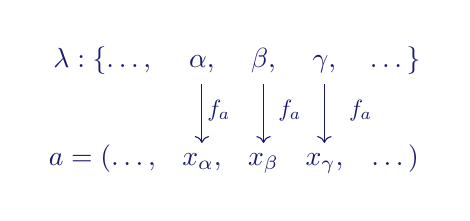
\begin{tikzpicture}[baseline= (a).base, color = MidnightBlue]
            \node[scale = 0.85] at (-0.2,0) {$f_a$};
            \node[scale = 0.85] at (0.7,0) {$f_a$};
            \node[scale = 0.85] at (1.6,0) {$f_a$};

            \node[scale=1] (a) at (0,0){
        \begin{tikzcd}[row sep=normal, column sep = 1.0, scale = 2]
            \lambda:\{ \dots, & \alpha, \arrow[d] & \beta\arrow[d], &
            \gamma\arrow[d],& \dots 
            \}
            \\
            a = (\dots, & x_\alpha, & x_\beta & x_\gamma, & \dots)  
        \end{tikzcd}
        };
    \end{tikzpicture}
    \end{center}
    \textcolor{NavyBlue}{
    The above diagram illustrates our descriptions so far, where
    in the case above we have that the $\alpha$-th element of $a$
    is $x_\alpha$, the $\beta$-th element of $a$ is $x_\beta$, and
    so on. With
    that said, we can now restate that 
    \[
        \prod_{\alpha \in \lambda} M_\alpha = \{\text{All functions } f \mid  f(\alpha) \in M_\alpha \text{ where } \alpha \in \lambda \}.
    \]
    and move onto understanding why we want to
    adjust our definition for multiplication of $R$-modules. 
    }

    It turns out that we can make the arbitrary cartesian product
    into an $R$-module. 

    \begin{proposition}
        If $\{M_\alpha\}_{\alpha \in \lambda}$ is a family of
        $R$-modules, then $\displaystyle \prod_{\alpha \in 
        \lambda}M_{\alpha}$ is an $R$-module.
    \end{proposition}

    \begin{prf}
        \begin{description}
            \item[Abelian Group.] First observe that $\displaystyle
            \prod_{\alpha \in \lambda} M_\alpha$ is an abelian group
            if we realize the identity is the zero map $f$ (i.e., the
            "tuple" of all zeros) and endow an operation of addition as follows. For
            $f_1,
            f_2 \in \displaystyle \prod_{\alpha \in \lambda} M_\alpha$
            we have that 
            \[
                (f_1 + f_2)(\alpha) = f_1(\alpha) + f_2(\alpha)
            \]
            for all $\alpha \in \lambda$. Note that this makes sense
            since $f_1(\alpha), f_2(\alpha) \in M_\alpha$. Hence the
            sum will be an element in $M_\alpha$. Also, if $f \in
            \displaystyle \prod_{\alpha \in \lambda} M_\alpha$, we
            define the inverse to be $f^{-1}$ where $f^{-1}(\alpha) =
            -f(\alpha)$. Commutativity is inherited from commutativity
            of all $M_\alpha$, and so we have an abelian group.

            \item[Ring Multiplication.] Let $a \in R$. Then define 
            \[
                (af)(\alpha) = a(f(\alpha))  
            \] 
            for all $\alpha \in \lambda$. Observe that, since each
            $M_\alpha$ is an $R$-module, we have that $f(\alpha) \in
            M_\alpha \implies af(\alpha) \in M_\alpha$ for all $\alpha
            \in \lambda$. Thus our multiplcation is well-defined. It is then a simple exercise to check that
            the axioms of an $R$-module are satisfied via our operations.
        \end{description}
    \end{prf}

    Since our above argument was a bit abstract, we reintroduce
    it in the language of finite products.
    Again, we can turn a finite cartesian product of
    $R$-modules into an $R$-module with the following operations.
\begin{itemize}
    \item[1.] Let $(m_1, m_2, \dots, m_n), (p_1, p_2 ,\dots,
    p_n) \in M_1 \times M_2 \times \cdots \times M_n$. Then let us define
    addition of elements as
    \[
        (m_1, m_2, \dots, m_n) + (p_1, p_2 ,\dots, p_n)
        = (m_1 + p_1, m_2 + p_2, \dots, m_n + p_n).
    \] 
    \item[2.] For any $a \in R$ and $(m_1, m_2, \dots, m_n) \in
    M_1 \times M_2 \times \cdots \times M_n$ we define scalar
    multiplication as 
    \[
        a(m_1, m_2, \dots, m_n) = (am_1, am_2, \dots, am_n).
    \] 
\end{itemize}
\end{definition}
Again, it is then simple to check that this satisfies the axioms
for an $R$-module. 

\textcolor{NavyBlue}{When we think of multiplying sets together,
cartesian products usually come to mind. They are the most natural
to us since it has been ingrained in us to think this way since
primary school. However, it turns out in many areas of mathematics
that the cartesian approach to defining multiplication of objects
leads to undersirable properties, and objects often misbehave
under a cartesian definition. 
\\
\\
As we said earlier, the problems arise when the products get
infinite. Hence the solution involves defining a new kind of
multiplication which is the same as a cartesian product for
\textit{finite} products, but is different for infinite products.}

This leads to the concept of direct sums, which we will use
instead of cartesian products (we will soon see why).

\begin{definition}
    Let $\{M_\alpha\}_{\alpha \in \lambda}$ be a family of
    $R$-modules. Then we define the \textbf{direct sum} of
    $\{M_\alpha\}_{\alpha \in \lambda}$ as 
    \[
        \bigoplus_{\alpha \in \lambda}M_\alpha = \{\text{All functions } f \mid f(\alpha) \in M_\alpha \textbf{ and } f(\alpha) = 0 \text{ except for finitely many } \alpha \in \lambda\}.
    \]
\end{definition}

The only
difference between the direct sum and the cartesian product is that, for any point
$\displaystyle a \in \bigoplus_{\alpha \in \lambda} M_\alpha$, all
indices of $a$ are zero except for finitely many indices. So
only finitely many indices are nonzero for a direct sum, while
in a cartesian product there may be finite, countable or
uncountably many nonzero indices.


\textcolor{purple}{Thus, note that for a finite product, the direct sum
and the cartesian product are the exact same thing}. There is no
difference when the product is finite. In other words, 
\[
    M_1 \times M_2 \times \cdots \times M_n = M_1 \oplus M_2 \oplus \cdots \oplus M_n.
\]

\begin{proposition}
    The direct sum of a family $\{M_\alpha\}_{\alpha \in
    \lambda}$ of $R$-modules is an $R$-module. In fact,
    $\displaystyle \bigoplus_{\alpha \in 
    \lambda} M_\alpha$ is an $R$-submodule of $\displaystyle \prod_{\alpha \in \lambda} M_{\alpha}$.
\end{proposition}

\begin{prf}
    Note that $\displaystyle \bigoplus_{\alpha \in \lambda}
    M_\alpha \subset \prod_{\alpha \in \lambda}M_\alpha$. Thus we
    can use the submodule test to check if is in fact an
    $R$-module. Observe that for any $a, b \in R$ and
    $\displaystyle f_1, f_2
    \in \bigoplus_{\alpha \in \lambda}M_{\alpha}$, we have that 
    \[
        a(f_1)(\alpha) + b(f_2)(\alpha) \in \bigoplus_{\alpha \in \lambda}M_{\alpha} 
    \]
    since the function $a(f_1)(\alpha) + b(f_2)(\alpha)$ will be
    nonzero for only finitely many values. (In fact, if $f_1$ is
    nonzero for $k$-many values and $f_2$ is nozero for $l$ many
    values, then $a(f_1)(\alpha) + b(f_2)(\alpha)$ is nonzero for
    at most $k + l$-many values). Hence this passes the submodule
    test.
\end{prf}

\noindent\textbf{Why do we prefer direct sums over cartesian products?} 
\\

The answer lies in the following observation. Suppose
$\{M_{\alpha}\}_{\alpha \in \lambda}$ is a family of $R$-modules and
that for each $\alpha \in \lambda$ there exists a homomorphism
$\phi_\alpha : M_\alpha \to N$. Let $a \in \displaystyle
\prod_{\alpha \in \lambda}M_\alpha$ and represent $a$ with the map
$f_a:\lambda \to \displaystyle \prod_{\alpha \in
\lambda}M_{\alpha}$. Thus $f_a(\alpha) \in M_\alpha$ is the $\alpha$-th
coordinate of our point $a$.

If we try to define
a homomorphism $\displaystyle \phi : \prod_{\alpha \in
\lambda}M_\alpha \to N$ in a natural, linear way such as 
\[
    \phi(a) = \sum_{\alpha \in \lambda}\phi_\alpha(f_a(\alpha))
\]
where $\displaystyle a \in \prod_{\alpha \in \lambda}M_{\alpha}$,
then observe that the above sum is nonsense. What the hell is an
infinite sum of module elements of $N$ supposed to represent?
Also, there's no way to make sure this is even well-defined!

However, if we instead consider $\displaystyle \bigoplus_{\alpha
\in \lambda}M_{\alpha}$, then creating a natural homomorphism
$\displaystyle \phi: \bigoplus_{\alpha \in 
\lambda}M_{\alpha} \to N$ where again 
\[
    \phi(a) = \sum_{\alpha \in \lambda}\phi_\alpha(f_a(\alpha))
\]
works out fine. We see that $\phi$ is valid because $f_a(\alpha) =
0$ for all but finitely many $\alpha \in \lambda$. Hence, the
above sum will only ever consist of a sum of finite elements.

The next important two theorems demonstrate the importance of the
direct sum.

\begin{thm}\label{fin_module_sums}
    Let $M$ be an $R$-module and suppose $M_1, M_2, \dots, M_n$
    are submodules such that 
    \begin{itemize}
        \item[1.] $M = M_1 + M_2 + \cdots + M_n$
        \item[2.] $M_j \cap (M_1 + M_2 + \cdots + M_{j-1} + M_{j +
        1} + \cdots + M_n) = \{0\}$ for all $j \in \{1, 2, \dots,
        n\}$. 
    \end{itemize}
    Then 
    \[
        M \cong M_1 \oplus M_2 \oplus \cdots \oplus M_n.
    \]
    \vspace{-0.8cm}
\end{thm}

\begin{prf}
    Construct the map $f:M_1 \oplus M_2 \oplus
    \cdots \oplus M_n \to M$ as 
    \[
        f(x_1, x_2, \dots, x_n) = x_1 + x_2 + \cdots + x_n.
    \]
    It is simple to check that this is an $R$-module homomorphism.
    Observe that by (1) $\im(f) = M$. Now suppose $(x_1, x_2, \dots, x_n) \in \ker(f)$. Then
    we see that 
    \[
        x_1 + x_2 + \cdots + x_n = 0 \implies x_i = -(x_1 + x_2 + \cdots + x_{i-1} + x_{i+1} + \cdots + x_n)
    \]
    for all $i \in \{1, 2, \dots, n\}$. But by (2), we know that
    no such $x_i$ can exist. Therefore $x_1 = x_2 = \cdots = x_n =
    0$. Hence, $f$ is an isomorphism, which yields the desired result.
\end{prf}

The above result can be generalized to arbitrary direct sums. However, if we
were dealing with cartesian products, we would not be able to
generalize the above theorem to arbitrary direct sums. 

\begin{thm}
    Let $M$ be an $R$-module and suppose $\{M_\alpha\}_{\alpha \in
    \lambda}$ is a family of $R$-modules such that 
    \begin{itemize}
        \item[1.] $\displaystyle M = \sum_{\alpha \in \lambda}
        M_\alpha$ 
        \item[2.] $M_\beta \bigcap \displaystyle  \sum_{\alpha \in
        \lambda\setminus\{\beta\}}M_\alpha = \{0\}$ for all $\beta
        \in \lambda$
    \end{itemize}
    then 
    \[
        M \cong \bigoplus_{\alpha \in \lambda}M_{\alpha}
    \]
    \vspace{-0.7cm}
\end{thm}

The proof is the exact same as before, although the notation is
annoying. 


\newpage
\section{Exact Sequences and the Hom Functor.}

This section will be the first encounter with the extremely
important algebraic concept of an \textit{exact sequence}, which
is something you may have already seen before without even knowing
it. 

\begin{definition}
    Let $R$ be a ring. We define a \textbf{sequence} of
    $R$-modules to be a chain of homomorphisms between
    $R$-modules, generally denoted as
    \begin{center}
        \begin{tikzcd}
            \cdots \arrow[r, "f_{i-1}"]
            &
            M_{i-1} \arrow[r, "f_{i}"]
            &
            M_i \arrow[r, "f_{i+1}"]
            &
            M_{i+1} \arrow[r, "f_{i+2}"]
            &
            \cdots
        \end{tikzcd}
    \end{center}
    we say that that the above sequence is \textbf{exact} at $M_i$
    if $\im(f_i) = \ker(f_{i+1})$. Hence, an exact sequence is a
    sequence which is exact at every $M_i$. 
\end{definition}

\noindent \textbf{Short Exact Sequences.}\\
Looking at "short" exact sequences aids out analysis of longer or
infinite exact sequences. 
\begin{proposition}
    Let $M_1, M_2$ and $M$ be $R$-modules. Then
    \begin{itemize}
        \item[1.] The sequence
        \begin{tikzcd}[column sep = \smallish]
            0 \arrow[r] & M_1 \arrow[r, "f"] & M     
        \end{tikzcd}
        is exact if and only if $f$ is injective.

        \item[2.] The sequence
        \begin{tikzcd}[column sep = \smallish]
            M \arrow[r, "g"] & M_2 \arrow[r] & 0    
        \end{tikzcd}
        is exact if and only if $g$ is surjective. 

        \item[3.] 
        The sequence
        \begin{tikzcd}[column sep = \smallish]
            0 \arrow[r] & M_1 \arrow[r, "f"] & M \arrow[r, "g"] & M_2 \arrow[r] & 0    
            \end{tikzcd} is exact if and only if $f$ is injective
            and $g$ is injective.
    \end{itemize}
\end{proposition}

\begin{prf}
    \begin{itemize}
        \item[1.]  
        ($\implies$) Suppose the sequence 
        \begin{tikzcd}[column sep = \smallish]
            0 \arrow[r] & M_1 \arrow[r, "f"] & M     
        \end{tikzcd}
        is exact. Then we have that $\im(0) = \ker(f) \implies
        \ker(f) = \{0\}$. Therefore we see that $f$ is injective. 

        ($\impliedby$)Now suppose $f$ is injective. Then $\ker(f) = 0$. Since
        $\im(0) = \{0\}$ we see $\im(0) = \ker(f)$, so that the
        sequence             \begin{tikzcd}[column sep = \smallish]
            0 \arrow[r] & M_1 \arrow[r, "f"] & M     
        \end{tikzcd}
        is exact.

        \item[2.] ($\implies$) Suppose the sequence 
        \begin{tikzcd}[column sep = \smallish]
            M \arrow[r, "g"] & M_2 \arrow[r] & 0    
        \end{tikzcd}
        is exact. Then we see that $\im(g) = \ker(0) = M_2$, since
        the zero map simply takes all of $M_2$ and sends it to $0$.
        Hence we see that $g$ is surjective. 

        ($\impliedby$) Now suppose $g$ is surjective. Then $\im(g)
        = M_2$ and we also have that $\ker(0) = M_2$. Therefore
        $\im(g) = \ker(0)$ so that we have an exact sequence. 

        \item[3.] By applying (1.) and (2.), the result follows.
    \end{itemize}
\end{prf}

The above proposition offers the following definitions. 

\begin{definition}
    Let $M_1, M_2$ and $M$ be $R$-modules. If the sequence
    \begin{center}
        \begin{tikzcd}[column sep = \smallish]
            0 \arrow[r] & M_1 \arrow[r, "f"] & M \arrow[r, "g"] & M_2 \arrow[r] & 0    
            \end{tikzcd} 
    \end{center}
    is exact then we say it forms an \textbf{short exact
    sequence}. Furthermore, if there exists an $R$-module $N$ such
    that $M = N \oplus \im(f) = N \oplus \ker(g)$ (since $\im(f) =
    \ker(g)$) then we say the above sequence is \textbf{split
    exact}.

    In this case, we say $N$ or $\im(f)$ is a \textbf{direct   
    summand} of $M$.
\end{definition}

We can offer a few short exact sequences with some familiar
objects. 
\\
\\
\textbf{Examples.}
\begin{itemize}
    \item[1.] Let $M$ be an $R$-module with a submodule $N$. If
    $i:N \to M$ is the inclusion map and 
    $\pi: M \to M/N$ is the projection map, then the sequence 
\begin{center}
    \begin{tikzcd}[column sep = \smallish]
        0 \arrow[r] & N \arrow[r, "i"] & M \arrow[r, "\pi"] & M/N \arrow[r] & 0    
        \end{tikzcd} 
\end{center}
is exact. \\
$\bm{\im(i) \subset \ker(\pi)}$. Observe
    that if $n \in N$ then 
    \[ 
        \pi(i(n)) = \pi(n) = n + N = N
    \]
    so that $\im(i) \subset \ker(g)$.
\\
$\bm{\ker(\pi) \subset \im(i)}$. Suppose $m
    \in \ker(\pi)$. Then we see that $\pi(m) = m + N = N$, so that
    $m \in N$. Since $m \in N$, we know that $i(m) = m$. Therefore
    $m$ is the image of some element in $M$ mapped by $i$ (namely,
    just $m$ itself). Hence $\ker(\pi) \subset \im(i)$.

With both directions, we can conclude that $\im(i) = \ker(\pi)$ so
so that the sequence is exact.

    \item[2.] Let $N$ and $P$ be $R$-modules. If we define $i':N
    \to N \oplus P$ where $i'(n) = (n, 0)$ and $\pi': N \oplus P
    \to P$ where $\pi'(n, p) = p$, we see that the sequence
    \begin{center} 
    \begin{tikzcd}[column sep = \smallish]
        0 \arrow[r] & N \arrow[r, "i'"] & N\oplus M \arrow[r, "\pi'"] & M \arrow[r] & 0    
        \end{tikzcd} 
    \end{center}
    is exact. We can realize this by simply observing that
    $\ker(\pi')$ is the set of all elements $(n, 0) \in N \oplus
    P$, which is exactly the image of $i'$. Therefore $\im(i') =
    \ker(\pi')$, so that the sequence is exact.

    \item[3.] The sequence
    \begin{center} 
        \begin{tikzcd}[column sep = \smallish]
            0 \arrow[r] & \ZZ_p \arrow[r, "f"] & \ZZ_{pq} \arrow[r, "g"] & \ZZ_q \arrow[r] & 0    
        \end{tikzcd} 
    \end{center}
    where $f:\ZZ_p \to \ZZ_{pq}$ is given by $f(n) = qn$ and
    $g: \ZZ_{pq} \to \ZZ_q$ is given by $g(n) = n \mbox{ mod } q$,
    then this sequence is exact. In fact, it is a split exact sequence.
    From group theory, we know that 
    \[
        \ZZ_{mn} \cong \ZZ_m \oplus \ZZ_n
    \]
    if and only if $m$ and $n$ are coprime. In our case, $p$ and
    $q$ are distint primes and hence are coprime so that $\ZZ_{pq} \cong \ZZ_p \oplus \ZZ_q$. We'll later show
    that this will be sufficient to conclude that this is a split
    sequence.

    \item[4.] If instead we have the sequence
    \begin{center} 
        \begin{tikzcd}[column sep = \smallish]
            0 \arrow[r] & \ZZ_p \arrow[r, "f"] & \ZZ_{p^2} \arrow[r, "g"] & \ZZ_p \arrow[r] & 0    
        \end{tikzcd} 
    \end{center}
    where $f:\ZZ_p \to \ZZ_{p^2}$ is given by $f(n) = pn$ and
    $g: \ZZ_{p^2} \to \ZZ_p$ is given by $g(n) = n \mbox{ mod }p$,
    then this becomes
    an exact sequence. However, this is not split exact as
    $p$ is obviously not comprime with itself, and hence 
    \[
        \ZZ_{p^2} \not\cong \ZZ_p \oplus \ZZ_p
    \]
    which is why this is not a split exact sequence. 
\end{itemize}

The last two examples can be generalized into a theorem, which
include other criterion for when a short exact sequence is split
exact. 

\begin{thm}\label{split_exact_lemma}
    Let $M_1, M_2$ and $M$ be $R$-modules such that 
    \begin{center}
        \begin{tikzcd}[column sep = \smallish]
            0 \arrow[r] & M_1 \arrow[r, "f"] & M \arrow[r, "g"] & M_2 \arrow[r] & 0    
            \end{tikzcd} 
    \end{center} 
    is exact. Then the following are equivalent:
    \begin{itemize}
        \item[1.] There exists a homomorphism $\alpha : M \to M_1$
        such that $\alpha \circ f = 1_{M_1}$ 
        \item[2.] There exists a homomorphism $\beta: M_2 \to M$
        such that $g \circ \beta = 1_{M_2}$ 
        \item[3.] The above sequence is split exact. 
    \end{itemize}
    Furthermore, we see that 
    \begin{align*}
        M &\cong \im(f) \oplus \ker(\alpha)\\
        &\cong \ker(g) \oplus \im(\beta)\\
        &\cong M_1 \oplus M_2.
    \end{align*} 
    \vspace{-.5cm}

\end{thm}




\begin{prf}
    \begin{description}
        \item[($\bm{1 \implies 3}$).] Suppose there exists an
        $\alpha : M \to M_1$ such that $\alpha \circ f = 1_{M_1}$.
        Let $m \in M_1$. Then observe that 
        \begin{align*}
            \alpha(m - f(\alpha(m))) &= \alpha(m) - \alpha(f(\alpha(m)))\\
            &= \alpha(m) - (\alpha \circ f)(\alpha(m))\\
            &= \alpha(m) - \alpha(m)\\
            &= 0
        \end{align*}
        where in the third step we used the fact that $\alpha
        \circ f = 1_{M_1}$, and hence $\alpha(f(m)) = m$ for all
        $m \in M_1$. Hence, $m - f(\alpha(m)) \in \ker(\alpha)$. 

        \begin{center}
            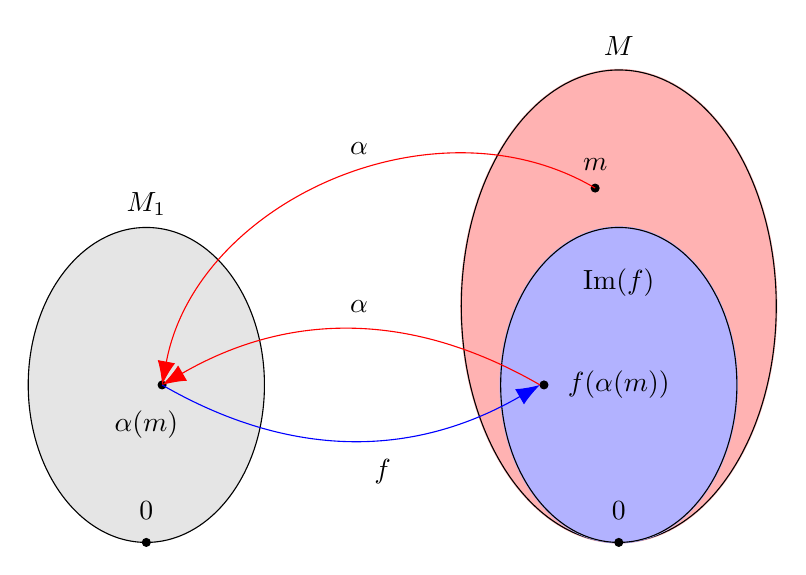
\begin{tikzpicture}
                \filldraw[gray!20] (-3, -1) ellipse (1.5cm and 2cm);
                \draw (-3, -1) ellipse (1.5cm and 2cm);
        
                \filldraw[thick, red!30] (3,0) ellipse (2cm and 3cm);
                \draw (3,0) ellipse (2cm and 3cm);
                \filldraw[thick, blue!30] (3,-1) ellipse (1.5cm and 2cm);
                \draw (3,-1) ellipse (1.5cm and 2cm);
        
                \filldraw (2.7, 1.5) circle (0.5mm); % m
                \node at (2.7, 1.8) {$m$};

                \filldraw (-2.8, -1) circle (0.5mm); % 
                \node at (-3, -1.5) {$\alpha(m)$};

                \filldraw (2.05, -1) circle (0.5mm); % a(f(m))
                \node at (3, -1) {$f(\alpha(m))$};

                \filldraw (-3, -3) circle (0.5mm);
                \filldraw (3, -3) circle (0.5mm);
        
                \draw[blue,-{Latex[length=3mm]}] (-2.8,-1) to [bend right] (2, -1);
                \draw[red, -{Latex[length=3mm]}] (2, -1) to [bend right] (-2.8,-1);
                \draw[red, -{Latex[length=3mm]}] (2.7, 1.5) to [bend
                right = 55] (-2.8, -1);

                \node at (3, 0.3) {$\im(f)$};
                \node at (-0.3, 0) {$\alpha$};
                \node at (-0.3, 2) {$\alpha$};
                \node at (0, -2.1) {$f$};
                \node at (-3, 1.3) {$M_1$};
                \node at (3, 3.3) {$M$};
                \node at (3, -2.6) {0};
                \node at (-3, -2.6) {0};
            \end{tikzpicture}

            \textit{$\alpha(m)$ and $\alpha(f(\alpha(m)))$ are mapped to
            the same element. Therefore, their difference is zero,
            so that $m - f(\alpha(m)) \in \ker(\alpha)$. }

        \end{center}
        Since $f: M_1 \to M$ is injective, we see that $\alpha: M
        \to M_1$ is surjective. To see this, let $m' \in M_1$.
        Then there exists an $m'' \in M$ such that $\alpha(m'') = m'$;
        namely, $m'' = f(m')$ works. 

        Since $\alpha$ is surjective, we see that 
        \[
            \{f(\alpha(m)) \mid m \in M\} = \{f(m_1) \mid m_1 \in M_1 \} = \im(f).
        \]
        That is, $f(\alpha(M)) = f(M_1) = \im(f)$.
        And because $\textcolor{red}{m - f(\alpha(m)) \in \ker(\alpha)}$ for all $m
        \in M$, we see that $m \in \im(f) + \ker(\alpha)$ for
        all $m \in M$. Hence, $M \subset \im(f) + \ker(\alpha)$.
        But both $\im(f)$ and $\ker(\alpha)$ are subsets of $M$.
        Therefore, $M = \im(f) + \ker(\alpha)$.     

        Now let $x \in \ker(\alpha) \cap \im(f)$. Then $f(y) = x$
        for some $y \in M_1$, and $\alpha(x) = 0$ as well. Hence, 
        \[
            \alpha(f(y)) = \alpha(x) = 0.
        \]
        But $\alpha \circ f = 0$, which implies that $y = 0$.
        Therefore $\ker(\alpha) \cap \im(f) = \{0\}$. 
        \begin{center}
            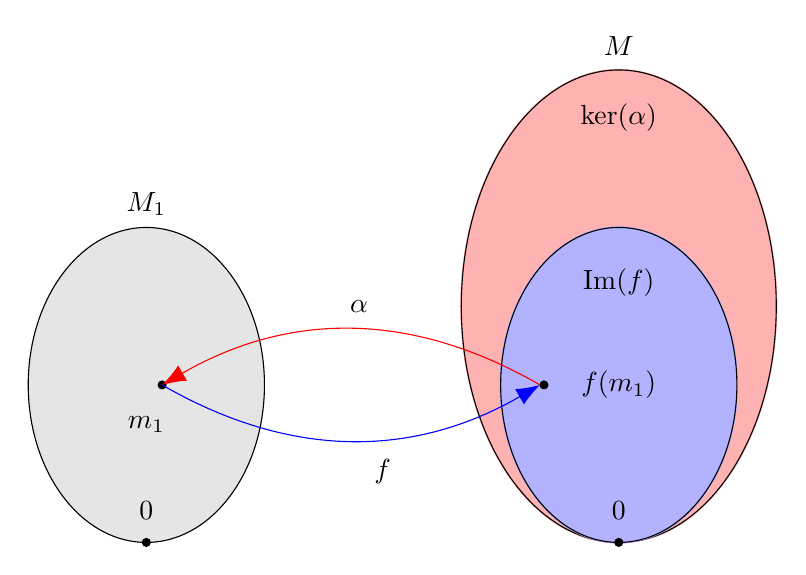
\begin{tikzpicture}
                \filldraw[gray!20] (-3, -1) ellipse (1.5cm and 2cm);
                \draw (-3, -1) ellipse (1.5cm and 2cm);
        
                \filldraw[thick, red!30] (3,0) ellipse (2cm and 3cm);
                \draw (3,0) ellipse (2cm and 3cm);
                \filldraw[thick, blue!30] (3,-1) ellipse (1.5cm and 2cm);
                \draw (3,-1) ellipse (1.5cm and 2cm);

                \filldraw (-2.8, -1) circle (0.5mm); % 
                \node at (-3, -1.5) {$m_1$};

                \filldraw (2.05, -1) circle (0.5mm); % a(f(m))
                \node at (3, -1) {$f(m_1)$};

                \filldraw (-3, -3) circle (0.5mm);
                \filldraw (3, -3) circle (0.5mm);
        
                \draw[blue, -{Latex[length=3mm]}] (-2.8,-1) to [bend right] (2, -1);
                \draw[red, -{Latex[length=3mm]}] (2, -1) to [bend right] (-2.8,-1);
                

                \node at (3, 0.3) {$\im(f)$};
                \node at (3, 2.4) {$\ker(\alpha)$};
                \node at (-0.3, 0) {$\alpha$};
                \node at (0, -2.1) {$f$};
                \node at (-3, 1.3) {$M_1$};
                \node at (3, 3.3) {$M$};
                \node at (3, -2.6) {0};
                \node at (-3, -2.6) {0};
            \end{tikzpicture}
        \end{center}
        By Theorem
        1.\ref{fin_module_sums}, we see that this implies that 
        \[
            M \cong \im(f) \oplus \ker(\alpha).
        \]
        Hence, $M$ is split exact as $\im(f)$ is a direct summand
        of $M$.

        

        \item[($\bm{2 \implies 3}$).] Suppose (2) holds. We'll show that $\textcolor{blue}{m - \beta(g(m)) \in \ker(g)}$ for all $m \in M$. 

        To show this, observe that 
        \begin{align*}
            g[m - \beta(g(m))] &=g(m) - g \circ \beta(g(m))\\
            &= g(m) - g(m)\\
            &= 0
        \end{align*}
        where in the second step we used the fact that $g \circ
        \beta = 1_{M_2}$. Therefore, $\textcolor{blue}{m -
        \beta(g(m)) \in \ker(g)}.$

        \begin{center}
            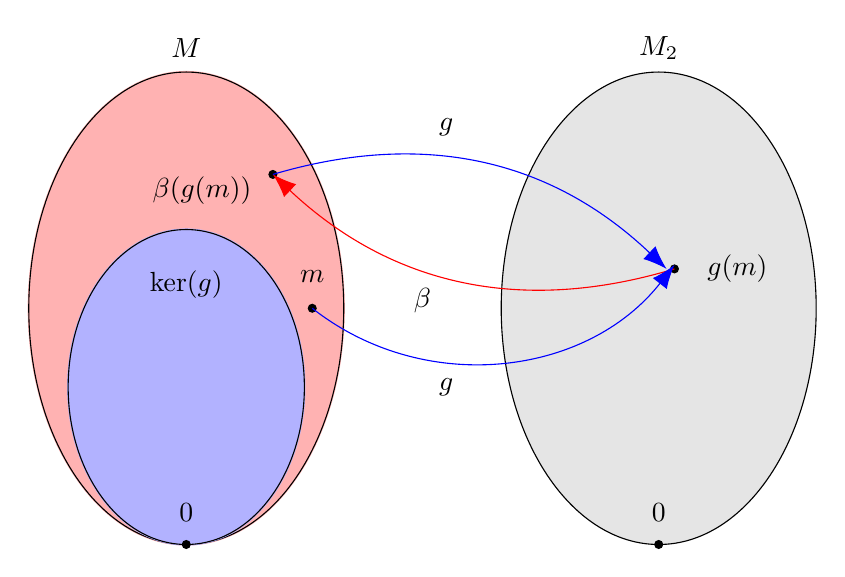
\begin{tikzpicture}[xscale=-1]
                    \filldraw[gray!20] (-3, 0) ellipse (2cm and 3cm);
                    \draw (-3, 0) ellipse (2cm and 3cm);
            
                    \filldraw[thick, red!30] (3,0) ellipse (2cm
                    and 3cm);
                    
                    \draw (3,0) ellipse (2cm and 3cm);

                    \filldraw[thick, blue!30] (3,-1) ellipse (1.5cm
                    and 2cm);
                    \draw (3,-1) ellipse (1.5cm and 2cm);
            
                    \filldraw (1.9, 1.7) circle (0.5mm); % m
                    \node at (2.8, 1.5) {$\beta(g(m))$};

                    \filldraw (-3.2, 0.5) circle (0.5mm); % 
                    \node at (-4, 0.5) {$g(m)$};

                    \filldraw (1.4, 0) circle (0.5mm); % a(f(m))
                    \node at (1.4, 0.4) {$m$};

                    \filldraw (-3, -3) circle (0.5mm);
                    \filldraw (3, -3) circle (0.5mm);
            
                    \draw[red,-{Latex[length=3mm]}] (-3.2,0.5) to
                    [bend right] (1.9, 1.7);
                    \draw[blue,-{Latex[length=3mm]}] (1.9, 1.7) to [bend
                    right] (-3.1,0.5);

                    \draw[blue,-{Latex[length=3mm]}] (1.4, 0) to [bend
                    left = 45] (-3.2, 0.55);

                    %\node at (3, 2.3) {$\im(\beta)$};
                    \node at (3, 0.3) {$\ker(g)$};
                    \node at (-0.3, 2.3) {$g$};
                    \node at (0, 0.1) {$\beta$};
                    \node at (-0.3, -1) {$g$};
                    \node at (-3, 3.3) {$M_2$};
                    \node at (3, 3.3) {$M$};
                    \node at (3, -2.6) {0};
                    \node at (-3, -2.6) {0};
            \end{tikzpicture}

            \textit{$g(m)$ and $g(\beta(g(m)))$ are mapped to the same element in $M_2$, so their difference is zero. Therefore, $m - \beta(g(m)) \in \ker(g).$}

        \end{center}
        
        Now note that 
        \[
            \{ \beta(g(m)) \mid m \in M\} = \{\beta(m_2) \mid m_2 \in M_2\} = \im(\beta)
        \]
        where in the second step we used the fact that $g$ is
        surjective. That is, $\beta(g(M)) = \beta(M_2) = \im(\beta)$. Therefore we see that 
        \[ 
            m \in \im(\beta) + \ker(g)
        \]
        for all $m \in M$ which implies that 
        $M \subset \im(\beta) + \ker(g)$. But since $\im(\beta)$
        and $\ker(g)$ are both subsets of $M$, we see that $M =
        \im(\beta) + \ker(g)$. 

        Now let $m' \in \im(\beta) \cap \ker(g)$. Then there
        exists an $m_2 \in M_2$ such that $\beta(m_2) = m'$.
        Furthermore, since $m' \in \ker(g)$, 
        \[
            0 = g(m') = g(\beta(m_2)) = m_2
        \]
        since $g \circ \beta = 1_{M_2}$. Hence, $m_2 = 0$, so that
        $\beta(m_2) = 0 = m$. Therefore $m = 0$, so that
        $\im(\beta) \cap \ker(g) = \{0\}$. 
        \begin{center}
            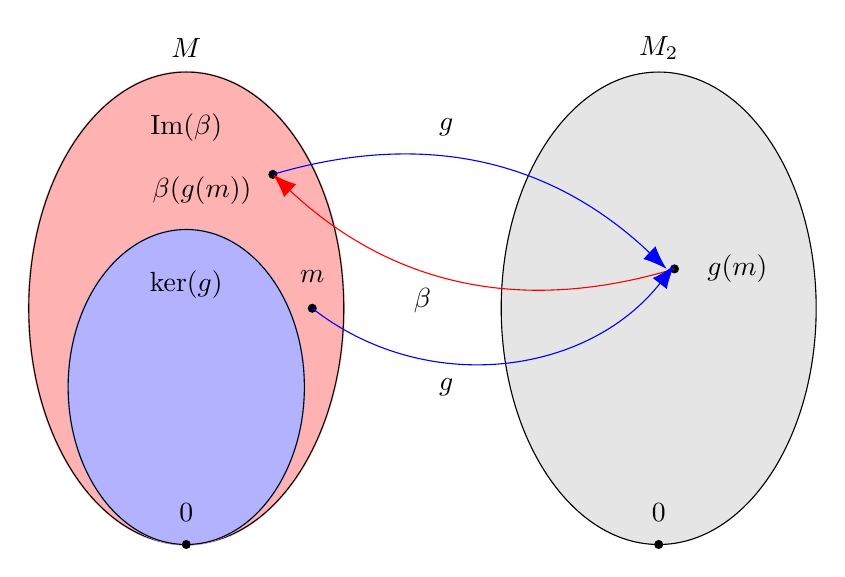
\begin{tikzpicture}[xscale=-1]
                    \filldraw[gray!20] (-3, 0) ellipse (2cm and 3cm);
                    \draw (-3, 0) ellipse (2cm and 3cm);
            
                    \filldraw[thick, red!30] (3,0) ellipse (2cm
                    and 3cm);
                    
                    \draw (3,0) ellipse (2cm and 3cm);

                    \filldraw[thick, blue!30] (3,-1) ellipse (1.5cm
                    and 2cm);
                    \draw (3,-1) ellipse (1.5cm and 2cm);
            
                    \filldraw (1.9, 1.7) circle (0.5mm); % m
                    \node at (2.8, 1.5) {$\beta(g(m))$};

                    \filldraw (-3.2, 0.5) circle (0.5mm); % 
                    \node at (-4, 0.5) {$g(m)$};

                    \filldraw (1.4, 0) circle (0.5mm); % a(f(m))
                    \node at (1.4, 0.4) {$m$};

                    \filldraw (-3, -3) circle (0.5mm);
                    \filldraw (3, -3) circle (0.5mm);
            
                    \draw[red,-{Latex[length=3mm]}] (-3.2,0.5) to
                    [bend right] (1.9, 1.7);
                    \draw[blue,-{Latex[length=3mm]}] (1.9, 1.7) to [bend
                    right] (-3.1,0.5);

                    \draw[blue,-{Latex[length=3mm]}] (1.4, 0) to [bend
                    left = 45] (-3.2, 0.55);

                    \node at (3, 2.3) {$\im(\beta)$};
                    \node at (3, 0.3) {$\ker(g)$};
                    \node at (-0.3, 2.3) {$g$};
                    \node at (0, 0.1) {$\beta$};
                    \node at (-0.3, -1) {$g$};
                    \node at (-3, 3.3) {$M_2$};
                    \node at (3, 3.3) {$M$};
                    \node at (3, -2.6) {0};
                    \node at (-3, -2.6) {0};
            \end{tikzpicture}

        \end{center}
        
        
        By Theorem
        1.\ref{fin_module_sums}, we have that 
        \[
            M \cong \im(\beta) \oplus \ker(g)
        \]
        so that $M$ is split exact, as one of its direct summands is $\ker(g)$.

        \item[($\bm{1 \implies 2}$).]
        Suppose (1) holds. Construct a function $\beta: M_2 \to M$
        defined by 
        \[
            \beta(u) = v - f(\alpha(v))
        \]
        where $g(v) = u$. Since $G$ is surjective, we know that
        such a $v$ exists, although we don't know if it is the
        only $v \in M$ which maps to $u$, and if that could cause
        us problems. Thus we'll show that
        this definition is well defined (i.e. independent of the
        choice of $v$). 

        \begin{description}
            \item[Well-defined.] 
            Suppose $g(v') = u$ for some other $v' \in M$. Then
            \begin{align*}
                g(v') - g(v) &= v - f(\alpha(v)) - (v' - f(\alpha(v')))\\
                &= (v - v') - f(\alpha(v)) + f(\alpha(v'))\\
                &= (v - v') - f(\alpha(v) - \alpha(v'))\\
                &= \textcolor{red}{(v - v') - f(\alpha(v - v'))}\\
                &= 0.
            \end{align*}
            We will prove the conclusion made in red, i.e., 
            $\textcolor{red}{(v - v') - f(\alpha(v - v'))} = 0.$
            \\

            To see this, first note that, as we proved earlier, $\textcolor{red}{x
            - f(\alpha(x))} \in \ker(\alpha)$
            for all $x \in M$. Hence, $\textcolor{red}{(v - v') - f(\alpha(v - v'))}
            \in \ker(\alpha)$. 
            \\

            Furthermore,
            since $g(v) = g(v')$, we see that $g(v - v')
            = 0 \implies v - v' \in \ker(g)$. But $\ker(g) = \im(f)$,
            so that $\textcolor{red}{v - v'} \in \im(f)$.
            Obviously $\textcolor{red}{f(\alpha(v - v'))} \in
            \im(f)$ for any $v \in M$, so that 
            $\textcolor{red}{(v - v') - f(\alpha(v - v'))}
            \in \im(f).$
            \\

            Thus we have that $\textcolor{red}{(v - v') - f(\alpha(v - v'))} \in \im(f)
            \cap \ker(\alpha) = \{0\}$, so that $g(v) - g(v') =
            0$.  
        \end{description}
        Next observe that for any $u \in M_2$ we have that 
        \begin{align*}
            g \circ \beta (u) &= g(v - f(\alpha(v)))\\
            &= g(v) - (g \circ f)(\alpha(v))\\
            &= g(v)
        \end{align*}
        where in the second step we used the fact that $(g \circ
        f) = 0$ as $\ker(g) = \im(f)$. Thus we have that $g \circ
        \beta = 1_{M_2}$, so that such a desired $\beta: M_2 \to M$
        exists. 

        \item[$\bm{(2 \implies 1)}$.] Suppose (2) holds. Construct
        a function $\alpha : M \to M_1$ defined by 
        \[
            \alpha(m) = f^{-1}(m - \beta (g(m))).
        \]
        Note that we must be careful since we're dealing with an
        inverse. To even make such a statement, we first recall
        that $f$ is injective, so an inverse from $f^{-1}: \im(f) \to M$
        certainly exists. But it only exists if its domain is at
        most $\im(f)$. Thus we check that $\textcolor{blue}{m - \beta(g(m)) \in
        \im(f)}$ for all $m \in M$.
        
        Earlier we proved that $\textcolor{blue}{m -
        \beta(g(m)) \in \ker(g)}$, and we know that $\ker(g) =
        \im(f)$ as the sequence is exact.
        Therefore, we already know that $\textcolor{blue}{m -
        \beta(g(m)) \in \im(f)}$.

        Hence, $\alpha$ makes sense
        since $f^{-1}$ exists and $m - \beta(g(m)) \in \im(f)$ for
        all $m \in M$.


        Now observe that for any $m_1 \in M_1$, 
        \begin{align*}
            \alpha \circ f(m_1) &= f^{-1}(f(m_1) - \beta(g(f(m_1))))\\
            &= f^{-1}f(m_1) - f^{-1}(0)\\
            &= m_1
        \end{align*}
        since $g(f(m_1)) = 0$ for all $m_1 \in M$. Thus such a
        desired $\alpha$ exists.

        \item[($\bm{3 \implies 1}$ \& 2).]
        Suppose that 
        \[
            M \cong M'\oplus M''
        \] 
        where $M' = \im(f) = \ker(g)$, and $M''$ is some other
        summand of $M$. Define a projection map $\pi: M \to M'$ as
        \[
            \pi(m) =
            \begin{cases}
                m & \text{ if } m \in M'\\
                0 & \text{ otherwise}
            \end{cases}
        \]
        and similarly the injective map $i: M'' \to M$ as $i(m'')
        = m''$ for all $m'' \in M$. 
        
        Consider $\pi \circ f: M \to M'$. Since $M' = \im(f)$,
        this is clearly an isomorphism. Now define $\alpha = (\pi
        \circ f)^{-1} \circ \pi_1$ and observe that $\alpha
        \to M \to M_1$ and 
        \[
            \alpha \circ f = (\pi \circ f)^{-1} \circ \pi_1 \circ f = 1_{M_1}.
        \]
        Hence, $(3) \implies (1)$.
        
        Similarly, observe that $g \circ i: M'' \to M_2$ is also
        an isomorphism. To see this, first observe that $M' =
        \ker(g)$, and since $M \cong M' \oplus M''$ we know that
        $M' \cap M'' = \{0\}$. Therefore, if $m \in M''$ is
        nonzero, then $m \not\in \ker(g)$. Hence $g(i(m)) \ne 0$
        if and only if $m = 0$, so that $g \circ i$ is one to one.
        Now surjectivity is clear, as $g$ itself is a surjective
        function. 

        Now define $\beta = i \circ (g \circ i)^{-1}$, and observe
        that $\beta : M_2 \to M$ and 
        \[
            g \circ \beta = g \circ i \circ (g \circ i)^{-1} = 1_{M_2}.
        \]
        Therefore $(3 \implies 2)$, which completes the entire proof.
    \end{description}
\end{prf}

That was a long ass proof, but the theorem is very powerful and
worthwhile. Next, we'll reintroduce the concept of $\hom()$.
\\

\noindent \textbf{Inducing Homomorphisms.}

\begin{minipage}{0.6\textwidth}
    Let $M, N$ and $N'$ be $R$-modules, and let $\phi: M \to N$ and $f: N
    \to N'$ be $R$-modules homomorphisms. Then we see that
    the diagram to the right commutes.

\end{minipage}
\hfill
\begin{minipage}{0.4\textwidth}
    \begin{center}
        \begin{tikzcd}[column sep = large, row sep = large]
            M \arrow[r, "\phi"] \arrow[rd, swap,"f \circ \phi"] & N \arrow[d, "f"]\\
            & N'
        \end{tikzcd}
    \end{center}
\end{minipage}
\vspace{0.5cm}

\begin{minipage}{0.6\textwidth}
    However, suppose we feed the above diagram with arbitrary $\phi: M
    \to N$. That is, we keep $f: N \to N'$ fixed, but let $\phi: M
    \to 
    N$ vary over all possible $\phi$. This is equivalent to grabbing
    elements from the abelian group $\hom_R(M, N)$. We can denote
    this with a red arrow, to remind the reader that this arrow
    "picks" $\phi$. 
\end{minipage}
\hfill
\begin{minipage}{0.4\textwidth}
    \begin{center}
        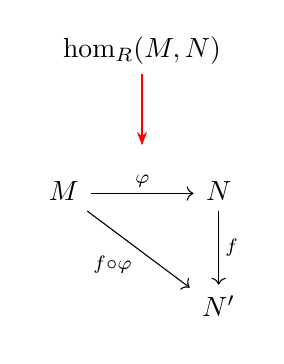
\begin{tikzpicture}
            \node at (0,2.5) {$\hom_R(M, N)$};
            \draw[red, ->] (0, 2.2) to (0, 1.3);
            \node{\begin{tikzcd}[column sep = large, row sep = large]
                M \arrow[r, "\phi"] \arrow[rd, swap, "f \circ \phi"]& N \arrow[d, "f"]\\
                & N'
            \end{tikzcd}};
        \end{tikzpicture}
    \end{center}
\end{minipage}

\begin{minipage}{0.6\textwidth}
    Note that we've described a well-defined system for assigning for each $\phi
    \in \hom_R(M, N)$ a function 
    \[ 
        f \circ \phi.
    \] 
    Also, $f \circ \phi
    : M \to N'$, so that $f \circ \phi \in \hom_R(M, N')$. We can
    denote this with a blue arrow, to communicate that
    $\hom_R(M,N')$ "accepts" $f \circ \phi$ (after all, it is an element of
    the set).
\end{minipage}
\hfill
\begin{minipage}{0.4\textwidth}
    \begin{center}
        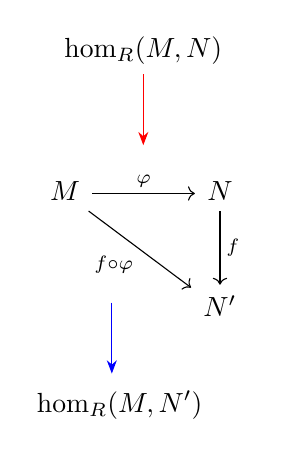
\begin{tikzpicture}
            \node at (0,2.5) {$\hom_R(M, N)$};
            \draw[red, ->] (0, 2.2) to (0, 1.3);
            \node{\begin{tikzcd}[column sep = large, row sep = large]
                M \arrow[r, "\phi"] \arrow[rd, swap, "f \circ \phi"]& N \arrow[d, "f"]\\
                & N'
            \end{tikzcd}};
            \draw[blue, ->] (-0.4, -0.7) to (-0.4, -1.6);
            \node at (-0.3, -2) {$\hom_R(M, N')$};
        \end{tikzpicture}
    \end{center}
\end{minipage}
\vspace{0.5cm}

\begin{minipage}{0.6\textwidth}
    What we've just described is an \textit{induced} function,
    which we denote as $f_*$.
    That is, if we fix $f$, then we can create a homomorphism
    $f_*$  between the abelian groups $\hom_R(M, N)$ and
    $\hom_R(M, N')$, where for each element $\phi \in \hom_R(M, N)$
    we assign it the function $f \circ \phi \in \hom_R(M, N')$.
\end{minipage}
\hfill
\begin{minipage}{0.4\textwidth}
    \begin{center}
        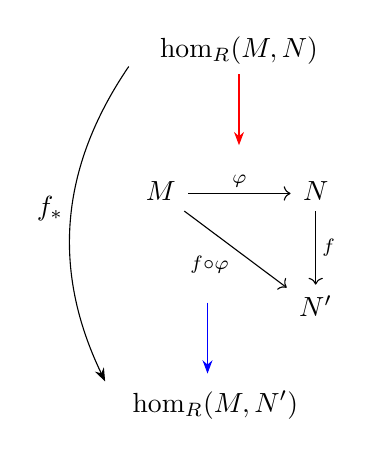
\begin{tikzpicture}
            \node at (0,2.5) {$\hom_R(M, N)$};
            \draw[red, ->] (0, 2.2) to (0, 1.3);
            \node{\begin{tikzcd}[column sep = large, row sep = large]
                M \arrow[r, "\phi"] \arrow[rd, swap, "f \circ \phi"]& N \arrow[d, "f"]\\
                & N'
            \end{tikzcd}};
            \draw[blue, ->] (-0.4, -0.7) to (-0.4, -1.6);
            \node at (-0.3, -2) {$\hom_R(M, N')$};
            \node at (-2.4, 0.5) {$f_*$};
            \draw[->] (-1.4, 2.3) to [bend right] (-1.7, -1.7);
        \end{tikzpicture}
    \end{center}
\end{minipage}


\noindent $\hom_R(- , M)$.\\
The we restate our results. If $N, N'$ are $R$-module homomorphisms and $f: N \to N'$ is an $R$-module
homomorphism, then for any $R$-module $M$ we can create an induced
homomorphism 
\[ 
    f_* : \hom_R(M, N) \to \hom_R(M, N')
\] 
defined as 
\[
    f_*(\phi) = f \circ \phi.
\]
\noindent $\hom_R(M, -)$.\\
Similarly, if $N, N'$ are again $R$-modules and $g: N' \to N$ is a an
$R$-module homomorphism, then for any $R$-module $M$, there is
an induced homomorphism 
\[
    g^*: \hom_R(N, M) \to \hom_R(N', M)
\]
defined as 
\[
    g^*(\psi) = \psi \circ g.
\]
It turns out in category theory that the behavior of these
functions fit the definition of a \textbf{functor}.
$\hom_R(- , M)$ is known as a covariant functor,
while $\hom_R(M, -)$ is known as a contravariant
functor. We won't delve too much into this.

\textcolor{NavyBlue}{Since the $\hom_R$ groups are abelian, we see that $f_*$ and $g_*$
are in fact group homomorphisms. If $R$ is commutative, then we
know that $\hom_R$ forms an $R$-module in which case $f_*$ and
$g_*$ become $R$-module homomorphisms.}
\\

Now suppose a family of $R$-modules $\{M_i \mid i \in \mathbb{N}\}$ associated with a
set of homomorphisms $\{f_i \mid f_i :M_{i-1} \to M_i, i
\in \mathbb{N}\}$ for a long sequence, not necessarily exact.
\begin{center}
    \begin{tikzcd}
        \cdots \arrow[r, "f_{i-1}"]
        &
        M_{i-1} \arrow[r, "f_{i}"]
        &
        M_i \arrow[r, "f_{i + 1}"]
        &
        M_{i+1} \arrow[r, "f_{i+2}"]
        &
        \cdots
    \end{tikzcd}
\end{center}
Then if we apply the $\hom_R(M, -)$ functor,
then we see that the above sequence implies a sequence between the
$\hom$ groups:
\begin{center}
    \begin{tikzcd}
        \cdots \arrow[r, "(f_{i-1})_*"]
        &
        \hom_R(M,M_{i-1}) \arrow[r, "(f_{i})_*"]
        &
        \hom_R(M,M_i) \arrow[r, "(f_{i+1})_*"]
        &
        \hom_R(M,M_{i+1}) \arrow[r, "(f_{i+2})_*"]
        &
        \cdots
    \end{tikzcd}
\end{center}
and applying the $\hom_R(-, M)$ functor we get 
\begin{center}
    \begin{tikzcd}
        \cdots
        &
        \hom_R(M,M_{i-1}) \arrow[l,swap, "(f_{i-1})^*"]
        &
        \hom_R(M,M_i) \arrow[l, swap,"(f_{i})^*"]
        &
        \hom_R(M,M_{i+1}) \arrow[l, swap,"(f_{i+1})^*"]
        &
        \cdots \arrow[l, swap, "(f_{i+2})^*"]
    \end{tikzcd}
\end{center}

Thus the long sequence of $R$-modules implies the existence of two other long
sequences of abelian groups. The interesting thing is that the two sequences are
similar but differ in the direction of the arrows (this is why we
denote the functions separately with an asterik either in the
subscript or superscript). Furthermore,
the direction of the arrows in the first seuqence of $M_i$
$R$-modules determines the direction of the arrows in the other
two sequences. 

\begin{thm}
    Let $M_1, M$ and $M_2$ be $R$-modules, and suppose $f:M_1 \to
    M$ and $g:M \to M_2$ are $R$-modules. Then the sequence
    \begin{equation}\label{0_M_1MM_2_short_exact}
        \begin{tikzcd}
            0 \arrow[r]
            &
            M_{1} \arrow[r, "f"]
            &
            M \arrow[r, "g"]
            &
            M_{2}
        \end{tikzcd}
    \end{equation}
    is exact if and only if the sequence 
        \begin{equation} \label{0_homM1_homM_homM2_exact_sequence}
        \begin{tikzcd}
            0 \arrow[r]
            &
            \hom_R(N,M_{1}) \arrow[r, "f_*"]
            &
            \hom_R(N, M) \arrow[r, "g_*"]
            &
            \hom_R(N,M_{2})
        \end{tikzcd}
    \end{equation}
    is an exact sequence of abelian groups. Furthermore, the sequence 
    \begin{equation}\label{M_1MM_2_0_short_exact}
        \begin{tikzcd}
            M_{1} \arrow[r, "f"]
            &
            M \arrow[r, "g"]
            &
            M_{2} \arrow[r]
            &
            0
        \end{tikzcd}
    \end{equation}
    is exact if and only if 
    \begin{equation}\label{homM1_homM_homM2_0_exact_sequence}
        \begin{tikzcd}
            \hom_R(M_{1}, N)
            &
            \hom_R(M, N) \arrow[l, swap, "f^*"]
            &
            \hom_R(M_{2}, N)\arrow[l, swap, "g^*"]
            & 
            0 \arrow[l]
        \end{tikzcd}
    \end{equation}
    is an exact sequence of abelain groups.
\end{thm}

\begin{prf}
    \textcolor{MidnightBlue}{To show that the sequence between the
    $\hom$ abelian groups is exact, we need to check that (1)
    $f_*$ is injective and (2) $\im(f_*) = \ker(g_*)$.
    }
    \begin{description}
        \item[$\bm{f_*}$ is injective.]
            Suppose that $f_*(\psi) = 0$ for some $\phi \in
            \hom_R(N, M_1)$. Then 
            \[
                f_*(\psi) = 0 \implies f(\psi(n)) = 0
            \] 
            for all $n \in M$. However, $f$ is injective, so that
            $\ker(f) = \{0\}$. Therefore $\psi(n) \in \ker(f) =
            \{0\}$ for all $n$, which means that $\psi$ is the
            zero function. Therefore $\ker(f_*) = \{0\}$ (where
            the zero here stands for the zero function between $N$
            and $M_1$) so that $f_*$ is injective. 

            \item[$\bm{\im(f_*) \subset \ker(g_*)}$.]
            Let $\phi \in \hom_R(N, M_1)$. Then observe that 
            \[
                g_*(f_*(\phi)) = g_*(f \circ \phi) = g \circ f \circ \phi = 0
            \] 
            since $g \circ f = 0$ as $\im(f) =
            \ker(g)$.
            Therefore we see that $\im(f_*) \subset \ker(g_*)$. 
    
            \item[$\bm{\ker(g_*) \subset \im(f_*)}$.]
            Let $\psi \in \hom_R(N, M)$ and suppose that $g_*(\psi)
            = 0$. Note that 
            \[
                g_*(\psi) = 0 \implies g(\psi(n)) = 0
            \]
            for all $n \in N$. Since $\ker(g) = \im(f)$, we know
            for all $n \in N$ that $\psi(n) \in \im(f)$.
            Therefore, there exist a set of $y \in M_1$ such that
            $f(y) = \psi(n)$, and since $f$ is one to one this
            correspondence is uniquely determined. 

            Thus construct a function $\tau: N \to M_1$ such that 
            \[
                \tau(n) = f^{-1}(\psi(n)).
            \]
            As we discussed, this function is well defined since
            $f$ is one-to-one, and therefore there is always a
            unique value of $f^{-1}(\psi(n))$ for each $n$. Now
            note that this function is an $R$-module homomorphism since, for
            any $n_1, n_2 \in N$ and $a \in R$  
            \begin{align*}
                \tau(n_1 + n_2) &=  f^{-1}(\psi(n_1 + n_2))\\
                &= f^{-1}(\psi(n_1) + \psi(n_2))\\
                &= f^{-1}(\psi(n_1)) + f^{-1}(\psi(n_2))\\
                &= \tau(n_1) + \tau(n_2)
            \end{align*}
            and 
            \begin{align*}
                \tau(an_1) &= f^{-1}(\psi(an_1))\\
                    &= f^{-1}(a\psi(n_1))\\
                    &= af^{-1}(\psi(n))\\
                    &= a\tau(n_1).
            \end{align*}
            Therefore we see that $\tau \in \hom_R(N_1, M)$ and that
            \[
                f_*(\tau) = f_*(f^{-1}(\psi)) = f(f^{-1}(\psi))= \psi.
            \]
            Hence, $\psi \in \im(f_*)$. Hence $\ker(g_*)
            \subset \im(f_*)$, which proves that $\ker(g_*) =
            \im(f_*)$.  
    \end{description}
    \textcolor{MidnightBlue}{To prove the reverse direction, we
    will assume the exactness of the second sequence and show that
    (1) $f$ is injective and (2) $\im(f) = \ker(g)$.}

    \begin{description}
        \item[$\bm{f}$ is injective.] Suppose that sequence
        \ref{0_homM1_homM_homM2_exact_sequence} is exact for all
        $R$-modules $N$. Then let $N = \ker(f)$, and since $N
        \subset M_1$ consider the
        inclusion map $i: N \to M_1.$  Note however that for any
        $n \in N$ we see that 
        \[
            f_*(i(n)) = f(i(n)) = 0
        \]
        since $\im(i) = \ker(f)$. Hence, $i \in \ker(f_*)$. 
        However, since $f_*: \hom_R(N,
        M_1) \to \hom_R(N, M)$ is injective, we know that
        $\ker(f_*) = 0$. Therefore we have that $i = 0$, (i.e. it
        is a zero map). But since we defined this to be the
        \textit{inclusion} map, we have that $N = \{0\}$. Hence,
        $\ker(f) = N = \{0\}$, so that $f$ is one to one.

        \item[$\im(f) \subset \ker(g)$.] 
        Let $N = M_1$, and let $1_{M_1}:M_1 \to M_1$ be the
        identity. Then we see that 
        \[
            0 = g_*(f_*(1_{M_1})) = g \circ f
        \]
        by exactness of sequence
        \ref{0_homM1_homM_homM2_exact_sequence}. Therefore we see
        that $\im(f) \subset \ker(g)$. 

        \item[$\ker(g) \subset \im(f)$.]
        
        


    \end{description}
\end{prf}

\begin{thm}
    Let $N$ be an $R$-module. If 
    \begin{center}
        \begin{tikzcd}
            0 \arrow[r]
            &
            M_{1} \arrow[r, "f"]
            &
            M \arrow[r, "g"]
            &
            M_{2} \arrow[r]
            &
            0
        \end{tikzcd}
    \end{center}
    is a split exact sequence of $R$-modules, then 
    \begin{center}
        \begin{tikzcd}
            0 \arrow[r]
            &
            \hom_R(N,M_{1}) \arrow[r, "f_*"]
            &
            \hom_R(N, M) \arrow[r, "g_*"]
            &
            \hom_R(N,M_{2}) \arrow[r]
            &
            0 
        \end{tikzcd}
    \end{center}
    and 
    \begin{center}
        \begin{tikzcd}
            0
            &
            \hom_R(M_{1}, N) \arrow[l]
            &
            \hom_R(M, N) \arrow[l, swap, "f^*"]
            &
            \hom_R(M_{2}, N)\arrow[l, swap, "g^*"]
            & 
            0 \arrow[l]
        \end{tikzcd}
    \end{center}
    are split exact sequences of abelian groups ($R$-modules if
    $R$ is commutative).
\end{thm}

\begin{prf}
    \textcolor{MidnightBlue}{By the previous theorem, we only need
    to show that $g_*$ and $f^*$ are surjective and that the two
    sequences split.
    }
    Since the first sequence splits, let $\beta: M_2 \to M$ be the
    function which splits the first sequence. Consider the
    function $\beta_*:
    \hom_R(N, M_2) \to \hom_R(N, M)$. 
    Then observe that for any $\psi \in \hom_R(N, M_2)$ that 
    \[
        g_* \circ \beta_* (\psi) = g_*(\beta(\psi)) = g \circ \beta(\psi) 
        = \psi.
    \]
    Therefore, we see that $g_* \circ \beta_* = 1_{\hom_R(M_{2}, N)}.$ Hence by
    Theorem 1.\ref{split_exact_lemma}, we see that $\beta_*$
    splits the second sequence. However, note also that $g_* \circ
    \beta_* = 1_{\hom_R(M_{2}, N)}$ implies that $g_*$ is surjective. Therefore
    the second sequence is split exact.
    \\

    As for the third sequence, consider the function $\alpha^*:
    \hom_R(M_1, N) \to \hom_R(M, N)$. Note that for any $\phi \in
    \hom_R(M, N)$, we have that 
    \[
        \alpha^* \circ f^*(\phi) = \alpha^*(f(\phi)) = \alpha \circ f(\phi) = \phi.
    \]
    Hence we see that $\alpha^* \circ f^*$ splits the third
    sequence. Furthermore, the fact that $\alpha^* \circ f^* =
    1_{\hom_R(M, N)}$ implies that $f^*$ is surjective. Thus in total
    we have that the third sequence is in fact a split exact sequence.
\end{prf}

The next theorem is a nice result that shows that $\hom_R$ is
somewhat of a "linear" operator.
\begin{thm}
    Let $M_1, M_2$ and $M$ be $R$-modules. Then 
    \[
        \hom_R(M, M_1\oplus M_2) \cong \hom_R(M, M_1)\oplus \hom_R(M, M_2)   
    \]
    and 
    \[
        \hom_R(M_1 \oplus M_2, M) \cong \hom_R(M_1, M) \oplus \hom_R(M_2, M).
    \]  
    \vspace{-0.7cm}
\end{thm}
These are in general isomorphisms of abelian groups, but can
be isomorphisms of $R$-modules if $R$ is commutative.

\begin{prf}
    Consider one of our earlier examples of a split exact
    sequences:
    \begin{center}
        \begin{tikzcd}
            0 \arrow[r]
            &
            M_{1} \arrow[r, "i"]
            &
            M_1\oplus M_2 \arrow[r, "\pi"]
            &
            M_{2} \arrow[r]
            &
            0
        \end{tikzcd}
    \end{center}
    where $i$ defined as $i(m_1) = (m_1, 0)$ is the inclusion map
    and $\pi$ defined by $\pi(m_1, m_2) = m_2$ is the projection
    map. As this is split exact, we can apply the previous theorem
    to gaurantee the existence of sequences 
    \begin{center}
        \begin{tikzcd}
            0 \arrow[r]
            &
            \hom_R(M,M_{1}) \arrow[r, "i_*"]
            &
            \hom_R(M, M_1\oplus M_2) \arrow[r, "\pi_*"]
            &
            \hom_R(M,M_{2}) \arrow[r]
            &
            0 
        \end{tikzcd}
    \end{center}
    and 
    \begin{center}
        \begin{tikzcd}
            0
            &
            \hom_R(M_{1}, M) \arrow[l]
            &
            \hom_R(M_1\oplus M_2, M) \arrow[l, swap, "i^*"]
            &
            \hom_R(M_{2}, M)\arrow[l, swap, "\pi^*"]
            & 
            0 \arrow[l]
        \end{tikzcd}
    \end{center}
    which are both split exact. Then by applying Theorem
    1.\ref{split_exact_lemma} we have that 
    \[
        \hom_R(M, M_1 \oplus M_2) \cong \hom_R(M, M_1) \oplus \hom_R(M, M_2)
    \]
    and 
    \[
        \hom_R(M_1 \oplus M_2, M) \cong \hom_R(M_1, M) \oplus \hom_R(M_2, M).
    \]
\end{prf}

\newpage
\section{Free $R$-modules.}
Free modules are the type of modules that you are probably
already familiar with. Basically, they're modules who have some
kind of generating set, which can create all other elements. As we
can think of modules as vector spaces, we know that vectors spaces
always have some kind of basis set, at least when they can be
thought of as existing in $\RR^n$. It turns out that having a
basis leads to many desirable properties. 

First, we make a definition on linear independence, a concept
required for discussing bases, and then formally define a free module.

\begin{definition}
    Let $R$ be a ring and $M$ an $R$-module. Then the set $S = \{x_1,
    x_2, \dots, x_n\}$ with $S \subset M$ is said to be
    \textbf{linearly independent} if and only if the only solution
    to the equation 
    \[
        a_1x_1 + a_2x_2 + \cdots + a_nx_n = 0
    \]
    is $a_1 = a_2 = \cdots = a_n = 0$ (where $a_1, a_2, \dots,
    a_n \in R$). 
    
    If $S$ is the smallest linear independent subset
    of $M$, then we say that $S$ is a \textbf{basis} for $M$, in
    which case $M$ is said to be a \textbf{free} $R$-module.
\end{definition}
Hence, an $R$-module is a module with a basis.

This is the exact same definition of linear independence we've
seen in linear algebra. 
Nothing is new here. It is a classic exercise in linear algebra to
check the following statement, which we offer here.

\begin{proposition}
    $S$ is a basis for some $R$-module $M$ if and only if every $x
    \in M$ can be written uniquely as 
    \[
        x = a_1x_1 + a_2x_2 + \dots a_nx_n
    \]
    where $a_i \in R$ and $x_i \in S$ for $i = 1,2, \dots, n$.
\end{proposition}

\textbf{Examples}
\begin{itemize}
    \item[1.] Consider the $R$-module $M_{m,n}(R).$ Observe that
    a basis for this module consists of 
    \[
        \{E_{ij} \mid 1 \le i \le m, 1 \le j \le n\}.
    \]

    \item[2.] Consider an abelian group $G$. Then as we showed
    before, $G$ is technically a $\mathbb{Z}$-module. However, if
    $G$ is finite, then it is not a free $\ZZ$-module. 
    
    
    Suppose to the contrary that it is, and that $S
    = \{x_1, x_2, \dots, x_n\}$ is a linearly independent set
    which forms a basis of $G$. Then if $\{o_1, o_2,
    \dots, o_n\}$ is a set such that $o_i = \text{order}(x_1)$
    (which exists, by finiteness of $G$) then  
    \[
        o_1x_1 + o_2x_2 + \cdots + o_nx_n = 0.
    \]
    Hence, the set $\{x_1, x_2, \dots, x_n\}$ is not linearly
    independent, so $G$ is not a free $\ZZ$-module.

    \item[3.] Consider the set $R[X]$. Observe that a suitable
    generating basis is 
    \[
        \{x^n \mid n \in \mathbb{N}\}
    \]
    which is probably something you already knew. 

    \item[4.] Suppose $M_1$ and $M_2$ are free modules with bases
    $S_1, S_2$. Then the set $M_1 \oplus M_2$ is a free module,
    since it has a basis 
    \[
        \{(x, 0) \mid x \in S_1\} \cup \{(0, y) \mid y \in S_2\}.
    \]
    More generally, if $\{M_\alpha\}_{\alpha \in \lambda}$ is a
    of free modules where $S_\alpha$ is the basis of $M_\alpha$,
    then we see that 
    \[
        \oplus_{\alpha \in \lambda}M_\alpha
    \]
    is also a free module with basis 
    \[
        \bigcup_{\alpha \in \lambda}\{(\delta_{jk}s_{j\alpha}) \mid s_{j\alpha} \in S_j\}.
    \]
    where $\delta_{jk}$ is the Kronecker delta function.
\end{itemize}

\begin{proposition}\label{prop: unique homomorphism}
    Let $M$ be a free $R$-module. Suppose the basis of the set is
    $S$. Let $N$ be an $R$-module and $h: S \to N$ a function.
    Then there exists a function $f \in \hom_R(M, N)$ such that
    $f\mid_S = h$. 
\end{proposition}

\begin{thm}
    Let $R$ be commmutative and $M$ and $N$ free modules with
    bases. Then $\hom_R(M, N)$ is a finitely generated free
    module. 
\end{thm}

\begin{prf}
    Suppose the basis for $M$ is $S = \{x_1, x_2, \dots, x_n\}$,
    and the basis for $N$ is $T = \{y_1, y_2, \dots, y_m\}$.
    Define a set of functions for $1 \le i \le m$ and $1 \le j \le
    n$ such that 
    \[
        f_{ij}(x_k) = 
        \begin{cases}
            y_j & \text{ if } k = i\\
            0 & \text{ if } k \ne j
        \end{cases}.
    \]
    By the previous proposition, we know that each $f_{ij}$ is a
    element in $\hom_R(M, N)$. Now let $f \in
    \hom_R(M,N)$ be arbitrary. Since $T$ is a basis for $N$, we
    know that for each $v_k \in S$ there exists coefficients
    $a_{k1}, a_{k2}, \dots, a_{kn}$ such that  
    \[
        f(v_k) = a_{k1}y_1 + \cdots + a_{kn}y_n.
    \]
    However, observe that 
    \begin{align*}
        f(v_k) &= a_{i1}y_1 + \cdots + a_{in}y_n\\
        &= a_{k1}f_{k1}(x_k) + a_{k2}f_{k2}(x_k) + \cdots + a_{kn}f_{kn}(x_k).
    \end{align*}
    Therefore, we see that for any $b \in M$, 
    \begin{align*}
        f(b) &= f(a_{b1}x_1 + \cdots + a_{bm}x_m)\\
        &=  a_{b1}f(x_1) + \cdots + a_{bm}f(x_m)\\
        &= a_{b1}[a_{11}f_{11}(x_1) + a_{12}f_{12}(x_1) + \cdots + a_{1n}f_{1n}(x_1)]\\
        &\hspace{.6cm} + a_{b2}[a_{21}f_{21}(x_2) + a_{22}f_{22}(x_2) + \cdots + a_{2n}f_{2n}(x_2)]\\
        &\hspace{.6cm} + \cdots\\
        &\hspace{.6cm} + a_{bm}[a_{m1}f_{m1}(x_m) + a_{m2}f_{m2}(x_2) + \cdots + a_{mn}f_{mn}(x_m)].
    \end{align*}
    Therefore we see that $\{f_{ij}\}$ generates $\hom_R(M, N)$,
    so that $\hom_R(M, N)$ is finitely generated.
\end{prf}
The previous theorem doesn't hold if $M$ and $N$ are not finitely
generated, since there are many counter examples to such a
claim. 
\textcolor{purple}{
Let $R = \mathbb{Z}$ and $M = \oplus_{i =
1}^{\infty}\mathbb{Z}$. Then observe that 
\[
    \hom_R(M, \ZZ) \cong \prod_{i = 1}^{\infty}\ZZ.
\]
by Theorem 1.13. However, we see that while $\ZZ$ is finitely 
generated and $M$ is finitely generated, but $\displaystyle \prod_{i =
1}^{\infty}\ZZ$ is not. (The proof is nontrivial.)}

\begin{proposition}
    Let $M$ be a free $R$-module with basis $S = \{x_j\}_{j \in
    J}$ and suppose $I$ is an ideal of $R$. Let $\pi: M \to M/I$.
    Then
    $M/IM$ is a $R/I$-module and is free with basis $\pi(S) = 
    \{ \pi(x_j)\}_{j \in J}$.
\end{proposition}

\begin{prf}
    \begin{description}
        \item[$\bm{M/IM}$ is an $\bm{R/I}$-module.]
        First recall that $IM$ is a submodule of $M$. Therefore it
        makes sense to consider the quotient $M/IM$. Then we can
        define a mapping $\cdot: R/I \times M/IM \to M/IM$ as follows. Let $r
        + I \in R/I$ and $m + IM \in M/IM$. Then define the mapping as
        \begin{align*}
            (r + I)\cdot(m + IM) &= r(m + IM)\\
            &= rm + rIM\\
            &= rm + IM.
        \end{align*}
        Since $M$ is an $R$-module, $rm \in M$ so that $rm + IM$ is in
        fact in $M/IM$. The other module properties may be easily
        verified without difficulty by using this mapping. 

        \item[$\bm{M/IM}$ is free.] 
        Suppose $m+ IM$ is an element of $M/IM$. Since $\pi: M \to
        M/I$ is a surjective mapping, we see that there exists at
        least one $m \in M$ such that $\pi(m) = m + IM$. Now since
        $m$ is free, there exists a unique representation of $m$
        of its basis elements, i.e., there exists $\{a_j\}_{j \in
        J}$, a subset of $R$, such that 
        \[
            m = \sum_{j \in J} a_jx_j \implies  \pi(m) = \pi\left(\sum_{j \in J} a_jx_j \right) =
            \sum_{j \in J} a_j\pi(x_j) + IM
        \]
        Hence $m + IM = \sum_{j \in J} a_j\pi(x_j) + IM.$ To finish showing
        that $\{\pi(x_j)\}_{j \in J}$ is a basis for $M/IM$, we
        only have to show that it is a linearly independent
        set. So consider the equation 
        \[
            \sum_{j \in J}a_j\pi(x_j) = 0 + IM                
        \]
        for some constants $\{a_j\}_{j \in J}$ in $\mathbb{R}$.
        Suppose additionally for contradiction that not all of the
        constants are nonzero. Then we that $\sum_{j \in
        J}a_j\pi(x_j)$ is an element of $IM$. However, this is a
        contradiction since none of the elements of
        $\{\pi(x_j)\}_{j \in J}$ is allowed to be in $IM$. Hence
        this set generates $M/IM$ and is linearly independent, so
        it is a basis.
    \end{description}
\end{prf}

We can introduce an even more useful proposition regarding free
modules, and more generally all modules. 

\begin{proposition}
    Let $M$ be an $R$-module. Then 
    \[
        M \cong F/K    
    \]
    for a free module $F$ and some submodule $K$ of $F$. That is,
    $M$ is the quotient of some free module $F$. Furthermore, if
    $M$ is finitely generated, then such an $F$ is finitely
    generated and $\mu(F) = \mu(M)$. 
\end{proposition}

\begin{prf}
    Suppose $S = \{x_j\}_{j \in J}$ is a set of elements which
    generate $M$. Note that, even in the worst case scenario, such
    an $S$ exists since we can at most take $S = M$. Now suppose
    $F = \oplus{j \in J}R$, which is a free module. Construct the
    module homomorphism $\psi: F \to M$ as 
    \[
        \psi((a_j)_{j \in J}) = \sum_{j \in J} a_jx_j.
    \]  
    Observe that since $S$ generates $M$, such a homomorphism is
    surjective onto $M$. Hence, we see that $M$ is the quotient of
    some free module $F$.

    Now suppose that $F$ is finitely generated. Then $S$ is a
    finite set, so that $F$ is also finitely generated (since in
    this case it is the direct sum of at most a finite number of
    copies of $R$). 

    Now if $M$ is finitely generated, and is a quotient of $F$,
    then clearly $\mu(M) \le \mu(F)$. However, we also know that
    $\mu(F) \le |J| \le \mu(M)$. Therefore, we see that $\mu(M) =
    \mu(F)$. 
\end{prf}

\begin{definition}
    Let $M$ be an $R$-module and $F$ a free $R$-module. Then the
    short exact sequence 
    \begin{center}
        \begin{tikzcd}
            0 \arrow[r] & K \arrow[r] & F \arrow[r] & M \arrow[r] & 0
        \end{tikzcd}
    \end{center}
    is called a \textbf{free presentation} of $M$. Note by the
    previous proposition that every $R$-module has a free
    presentation. 
\end{definition}

Presentations are particularly useful since they make free modules
convenient to work with. 

\begin{proposition}
    Suppose $F$ is a free $R$-module. Then every short exact
    sequence 
    \begin{center}
        \begin{tikzcd}
            0 \arrow[r] & M_1 \arrow[r] & M \arrow[r] & F \arrow[r] & 0
        \end{tikzcd}
    \end{center}
    is a split exact sequence. 
\end{proposition}

\begin{prf}
    Let $S = \{x_j\}_{j \in J}$ be a basis for $F$. Now suppose $f: M \to F$ is the
    surjective function in the above exact sequence. Now construct
    a function $\psi: F \to M$ as follows: $\psi(x_j) = m_j$ if
    and only if $f(m_j) = x_j$. Since $f$ is surjective, note that
    this will always be possible. Such a function may not be
    unique, but we don't care; we just want to know it exists. 

    By proposition \ref{prop: unique homomorphism}, we know that
    there exists a unique function $h: F \to M$ such that $h|_S =
    \psi$. Therefore we see that $f \circ h = 1_F$, so that by
    theorem \ref{split_exact_lemma}, we see that the sequence is
    in fact split exact. 
\end{prf}


\end{document}